\documentclass[a4paper,12pt, oneside]{book}

% \usepackage{fullpage}
\usepackage[italian]{babel}
\usepackage[utf8]{inputenc}
\usepackage{amssymb}
\usepackage{amsthm}
\usepackage{graphics}
\usepackage{amsfonts}
\usepackage{listings}
\usepackage{amsmath}
\usepackage{amstext}
\usepackage{engrec}
\usepackage{rotating}
\usepackage{verbatim}
\usepackage[safe,extra]{tipa}
%\usepackage{showkeys}
\usepackage{multirow}
\usepackage{hyperref}
\usepackage{microtype}
\usepackage{fontspec}
\usepackage{enumerate}
\usepackage{physics}
\usepackage{braket}
\usepackage{multicol}
\usepackage{marginnote}
\usepackage{pgfplots}
\usepackage{cancel}
\usepackage{polynom}
\usepackage{booktabs}
\usepackage{enumitem}
\usepackage{framed}
\usepackage{pdfpages}
\usepackage{pgfplots}
\usepackage{algorithm}
\usepackage{manfnt}
% \usepackage{algpseudocode}
\usepackage[cache=false]{minted}
\usepackage{mathtools}
\usepackage[noend]{algpseudocode}

\usepackage{tikz}\usetikzlibrary{er}\tikzset{multi  attribute /.style={attribute
    ,double  distance =1.5pt}}\tikzset{derived  attribute /.style={attribute
    ,dashed}}\tikzset{total /.style={double  distance =1.5pt}}\tikzset{every
  entity /.style={draw=orange , fill=orange!20}}\tikzset{every  attribute
  /.style={draw=MediumPurple1, fill=MediumPurple1!20}}\tikzset{every
  relationship /.style={draw=Chartreuse2,
    fill=Chartreuse2!20}}\newcommand{\key}[1]{\underline{#1}}
  \usetikzlibrary{arrows.meta}
  \usetikzlibrary{decorations.markings}
  \usetikzlibrary{arrows,shapes,backgrounds,petri}
\tikzset{
  place/.style={
        circle,
        thick,
        draw=black,
        minimum size=6mm,
    },
  transition/.style={
    rectangle,
    thick,
    fill=black,
    minimum width=8mm,
    inner ysep=2pt
  },
  transitionv/.style={
    rectangle,
    thick,
    fill=black,
    minimum height=8mm,
    inner xsep=2pt
    }
  } 
\usetikzlibrary{automata,positioning,chains,fit,shapes}
\usepackage{fancyhdr}
\pagestyle{fancy}
\fancyhead[LE,RO]{\slshape \rightmark}
\fancyhead[LO,RE]{\slshape \leftmark}
\fancyfoot[C]{\thepage}
\usepackage[usenames,dvipsnames]{pstricks}
\usepackage{epsfig}
\usepackage{pst-grad} % For gradients
\usepackage{pst-plot} % For axes
\usepackage[space]{grffile} % For spaces in paths
\usepackage{etoolbox} % For spaces in paths
\makeatletter % For spaces in paths
\patchcmd\Gread@eps{\@inputcheck#1 }{\@inputcheck"#1"\relax}{}{}
\makeatother

\title{Teoria dell'Informazione e Crittografia}
\author{UniShare\\\\Davide Cozzi\\\href{https://t.me/dlcgold}{@dlcgold}}
\date{}

\pgfplotsset{compat=1.13}
\begin{document}
\maketitle

\definecolor{shadecolor}{gray}{0.80}
\setlist{leftmargin = 2cm}
\newtheorem{teorema}{Teorema}
\newtheorem{definizione}{Definizione}
\newtheorem{esempio}{Esempio}
\newtheorem{corollario}{Corollario}
\newtheorem{lemma}{Lemma}
\newtheorem{osservazione}{Osservazione}
\newtheorem{nota}{Nota}
\newtheorem{esercizio}{Esercizio}
\algdef{SE}[DOWHILE]{Do}{doWhile}{\algorithmicdo}[1]{\algorithmicwhile\ #1}
\tableofcontents
\renewcommand{\chaptermark}[1]{%
  \markboth{\chaptername
    \ \thechapter.\ #1}{}}
\renewcommand{\sectionmark}[1]{\markright{\thesection.\ #1}}
\newcommand{\floor}[1]{\lfloor #1 \rfloor}
\newcommand{\MYhref}[3][blue]{\href{#2}{\color{#1}{#3}}}%
\chapter{Introduzione}
\textbf{Questi appunti sono presi a lezione. Per quanto sia stata fatta
  una revisione è altamente probabile (praticamente certo) che possano
  contenere errori, sia di stampa che di vero e proprio contenuto. Per
  eventuali proposte di correzione effettuare una pull request. Link: }
\url{https://github.com/dlcgold/Appunti}.\\
\chapter{Introduzione agli argomenti del corso}
Si ha una sorgente che emette messaggi e li vuole mandare tramite un canale di
comunicazione, che contiene del rumore che agisce sui messaggi e li rovina. Il
destinatario per capire che il messaggio è rovinato ha varie tecniche. Una
prima cosa che potrebbe fare è chiedere di rimandare il messaggio ma sarebbe
meglio correggere \textit{in loco} e si hanno algoritmi per farlo (tra cui lo
\textbf{schema di Hamming} usando il modello del \textbf{rumore bianco}).\\
Un'altra tematica è la codifica stessa del sorgente, comprimendo flussi di dati,
senza perdere informazioni.\\
Si parlerà anche dei canali di comunicazione, delle capacità e dei
\textbf{teoremi di Shannon}. \\
Si vedranno poi le basi della crittografia, i crittosistemi storici, vari
standard etc$\ldots$
\chapter{Teoria dell'informazione}
Si hanno due sottoparti principali:
\begin{itemize}
  \item \textbf{teoria dei codici}, per individuare e correggere gli errori. Si
  studia il canale di trasmissione cercando di contrastare il rumore che c'è nel
  canale
  \item \textbf{teoria dell'informazione}, in cui il focus è la sorgente delle
  informazioni
\end{itemize}
Vediamo il classico schemino della teoria dell'informazione:
\begin{figure}[H]
  \centering
  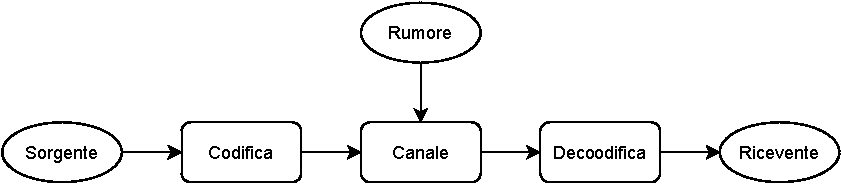
\includegraphics[width = \textwidth]{img/teo.pdf}
  \caption{Schema di un sistema generale di comunicazione tipico della teoria
    dell'informazione} 
  \label{fig:teo}
\end{figure}
Avendo:
\begin{itemize}
  \item la \textbf{sorgente} che produce segnali, dei simboli, che potrebbero
  essere continui (come la corrente), anche se noi li assumeremo come simboli di
  un alfabeto finito, avendo quindi una \textbf{sorgente discreta}
  \item i simboli, per poter essere spediti all'interno di un canale, vanno
  codificati, avendo una parte di \textbf{codifica}
  \item una volta codificati i simboli vanno nel \textbf{canale di
    trasmissione}, dove si ha del \textbf{rumore}. Tale \textit{rumore} prende
  un simbolo di quelli inseriti e lo cambia
  \item dal canale esce o il simbolo che è entrato o il simbolo modificato dal
  rumore e, tipicamente, non è immediatamente utilizzabile ma deve passare per
  una fase di \textbf{decodifica}
  \item il simbolo decodificato arriva al \textbf{destinatario}
\end{itemize}
Si hanno
alcune assunzioni sulla sorgente:
\begin{itemize}
  \item è \textbf{discreta}, i simboli emessi appartengono ad un alfabeto
  finito. Normalmente tali simboli sono $S=\{s_1, s_2,\ldots,s_q\}$
  \item i simboli vengono emessi uno alla volta ad ogni \textbf{colpo di
    clock}. Non si ha mai che in un colpo di clock non escano simboli o che ne
  escano più di uno solo 
  \item la sorgente è \textbf{senza memoria (\textit{memoryless})}, avendo che
  i simboli già usciti non influenzano per nulla il simbolo che sta per
  uscire. Ogni simbolo che esce non tiene conto del passato, \textit{è come se
    fosse il primo}
  \item è \textbf{probabilistica e randomizzata}. Si ha quindi che i simboli
  $S=\{s_1, s_2,\ldots,s_q\}$ escono con le probabilità
  $(p_1,p_2,\ldots,p_q)$. Deve valere che, ovviamente, che $p_i\in
  [0,1],\forall
  i=1,\ldots,q$. Si ha inoltre che le varie probabilità, nel loro insieme,
  devono formare una distribuzione di probabilità, avendo che:
  \[\sum_{i=1}^q p_i=1\]
  Potrei avere simboli con probabilità nulla di comparire ma nella pratica non
  è qualcosa di sensato. La sorgente la costruisco o da zero (e a quel punto
  un simbolo con probabilità nulla non lo metterei) o ho una sorgente che devo
  studiare (e qui potrei avere simboli con probabilità bassissime se non
  nulle, in tal caso bisognerebbe rivalutare l'assunzione dei simboli di
  quella sorgente). Possiamo quindi meglio dire che $p_i\in (0,1],\forall
  i=1,\ldots,q$.\\
  D'altro canto vedo se posso avere probabilità pari a 1 per un simbolo ma in
  tal caso avrei solo quello e non sarebbe interessante. Si ha quindi che:
  \[p_i\in (0,1),\forall i=1,\ldots,q\]
  \[\sum_{i=1}^q p_i=1\]
  \textit{Le sorgenti che emettono i simboli secondo  
    uno schema prefissato, deterministico, sono poco interessanti, avendo un
    comportamento banale}
\end{itemize}
Il concetto di \textit{spedire in un canale} può anche essere generalizzato in
altre ``idee'', come il disco su cui salvo dei dati e il tempo per cui li
salvo.\\ 
La parte di \textit{codifica e decodifica} può essere approfondita. Nello schema
in figura \ref{fig:teo} ci si è infatti concentrati sul canale, avendo che la
codifica serve a fare in modo che il simbolo trasmesso vada bene per essere
trasmesso nel canale. La \textbf{codifica} è a sua volta suddivisa in due parti:
\begin{enumerate}
  \item \textbf{codifica di sorgente}, che ha come obiettivo rappresentare nel
  modo più efficiente e compatto i simboli emessi dalla \textit{sorgente}. Si
  vuole quindi comprimere la sequenza di simboli (messaggi) emessi dalla
  sorgente, per impegnare meno banda possibile quando andremo a spedire. Si deve
  considerare che ogni bit in un file 
  compresso è essenziale per permettere di poter recuperare il contenuto
  compresso 
  \item \textbf{codifica di canale}, che ha quasi uno scopo opposto rispetto
  alla \textit{codifica di sorgente}, infatti ha come obiettivo quello di
  contrastare il rumore e per farlo aggiunge ridondanza al messaggio (da qui il
  discorso sull'obiettivo opposto)
\end{enumerate}
Si cerca quindi di comprimere il più possibile nella prima fase, quella di
\textit{codifica di sorgente} e di ridondare il meno possibile nella seconda,
quella di \textit{codifica di segnale}.\\
Per capire meglio quanto detto diamo alcune formalità.
\begin{definizione}
  Una \textbf{codifica} è una funzione $cod$ che prende i simboli della sorgente
  $S=\{s_1, s_2,\ldots,s_q\}$ e ad ogni simbolo $s_i$ gli assegna una stringa
  formata coi caratteri di un certo alfabeto $\Gamma$, l'\textbf{alfabeto
    della codifica}. Le stringhe di $\Gamma^*$ sono tutte quelle costruite
  sull'alfabeto $\Gamma$ di lunghezza arbitraria e finita, compresa la stringa
  vuota $\varepsilon$, che posso quindi formare coi simboli di $\Gamma$. Quindi
  ad ogni $s_i\in S$ assegno un $\gamma_i\in Gamma^*$, avendo che:
  \[cod:S\to \Gamma^*\]
  generalmente si ha che:
  \[|\Gamma|<|\Sigma|\]
  e quindi i simboli di $\Sigma$ sono mappati da $cod$ in  sequenze  di  simboli
  di $\Gamma$, a meno che non si ritenga accettabile il fatto che due o più
  simboli di $\Sigma$ vengano mappati nellostesso simbolo di $\Gamma$. \\
  \textit{Più avanti nel corso vedremo casi in cui $|\Gamma|>|\Sigma|$}
\end{definizione}
Si hanno quindi i simboli $S=\{s_1, s_2,\ldots,s_q\}$ che escono con
probabilità $(p_1,p_2,\ldots,p_q)$ e che vengono codificati con le stringhe
$\gamma_1,\gamma_2,\ldots,\gamma_q$. Le varie $gamma_i$ sono dette
\textbf{codeword}. Chiamando $l_i=|\gamma_i|$ la lunghezza 
di tali stringhe si ha che tali stringhe hanno associati i vari
$l_1,l_2,\ldots,l_q$.\\
L'obiettivo quindi della \textit{codifica di sorgente} è quello di minimizzare
la lunghezza media $L$ delle stringhe, avendo quindi una media pesata (pesata
sulle probabilità):
\[L=\sum_{i=1}^q p_i\cdot l_i\]
Tenendo conto delle probabilità, per minimizzare $L$, si deve, avendo a che fare
con termini che sono tutti $>0$ (avendo supposto che non si hanno probabilità
nulla e avendo che una codeword pari alla stringa vuota ha poco senso), fare in
modo che i termini siano tutti il più piccolo possibile. Dato che le probabilità
sono date mentre la codifica la sto costruendo, calcolando le codeword e di
conseguenza le loro lunghezze, devo fare in modo che se la probabilità è grande
la lunghezza deve essere piccola. Se invece la probabilità è piccola posso
permettermi una lunghezza più grande. Parto quindi dai simboli con probabilità
più grande e inizio a usare codeword più piccole possibili, usando via via
quelle più lunghe. \\
Un'idea simile è usata nel \textit{codice Morse} dove le
lettere meno comuni hanno le sequenze più lunghe di punti, linee e spazi (avendo
una codifica ternaria). La lettera più comune, la ``e'', ha infatti solo con un
punto, la codifica più breve mentre le meno comuni hanno sequenze multiple di
punti, linee e spazi che le separano (e gli spazi contano nella lunghezza di
queste codeword).\\
Noi non sappiamo in anticipo che messaggi verranno prodotti dalla sorgente e
quindi le codeword vanno studiate passo a passo, valutando i simboli più
probabili per associare le codeword più brevi e i meno probabili per le
codeword più lunghe.\\
Analizziamo meglio i codici, le codeword. Possono essere:
\begin{enumerate}
  \item \textit{a lunghezza fissa}, ovvero si ha che $l_1=l_2=\cdots=L_q$
  \item \textit{a lunghezza variabile}, avendo che ogni codeword può avere
  lunghezza diversa
\end{enumerate}
Ne segue quindi che il discorso di minimizzare $L$ ha senso solo in presenza di
\textit{codeword a lunghezza variabile} (potendo decidere per ogni simbolo che
codeword associare), avendo la \textbf{codifica a lunghezza variabile}.\\
Con \textit{codeword a lunghezza fissa} avrei tutte le $l_i$ uguali e quindi
avrei, avendo $l_i=l,\forall i$:
\[L=\sum_{i=1}^q p_i\cdot l_i \sum_{i=1}^q p_i\cdot l =l\cdot\sum_{i=1}^q
  p_i=l\cdot 1 = l\]
avendo, come facilmente intuibile, che la lunghezza media è la lunghezza fissa
stessa. Si hanno codifiche a lunghezza fissa, come banalmente numeri a 64bit
etc$\ldots$ in tal caso si parla di \textbf{codici a blocchi}.\\
Usando codifiche a lunghezza fissa si hanno anche esempi interessanti come
quello del \textit{codice pesato}, detto \textbf{codice pesato 01247}. Il nome
deriva dal fatto che si possono codificare le cifre da 0 a 9 (da 1 a 9 con poi
lo 0 dopo il 9) sotto forma di stringhe di 5 bit usando i pesi 0,1,2,4,7
associati a ciascun bit. Vediamo la tabella con la codifica di questo codice:
\begin{table}[H]
  \centering
  \begin{tabular}{c|ccccc} 
    & 0 & 1 & 2 & 4 & 7 \\
    \hline
    1 & 1 & 1 & 0 & 0 & 0 \\
    2 & 1 & 0 & 1 & 0 & 0 \\
    3 & 0 & 1 & 1 & 0 & 0 \\
    4 & 1 & 0 & 0 & 1 & 0 \\
    5 & 0 & 1 & 0 & 1 & 0 \\
    6 & 0 & 0 & 1 & 1 & 0 \\
    7 & 1 & 0 & 0 & 0 & 1 \\
    8 & 0 & 1 & 0 & 0 & 1 \\
    9 & 0 & 0 & 1 & 0 & 1 \\
    0 & 0 & 0 & 0 & 1 & 1
  \end{tabular}
\end{table}
Si nota che ogni codeword ha sempre 3 bit pari a 0 e due bit pari a 1, avendo un
\textbf{codice 2-su-5}. Banalmente i pesi si associano ai numeri 0,1,2,4,7 in
modo tale che essi, sommati, formino il numero voluto (ad esempio per 1 avrò i
pesi su 0 e 1, per 9 su 2 e 7 etc$\ldots$). L'unico caso è il caso dello 0, che
non può essere ottenuto come somma di due pesi (spesso si hanno nei codici casi
speciali da gestire a parte). Per lo 0 viene quindi presa una codeword non usata
per altri numeri e quindi l'unica scelta possibile è avere i pesi su 4 e 7
(visto che farebbe 11).\\
Su un totale ci 5 bit, avendo due bit a 1 e tre bit a 0, posso avere un numero
di codeword pari a:
\[n={{5}\choose{2}}=10\]
avendo che i 5 bit sono associati ai 5 elementi dove 1 segnala che ``sto usando
quel peso'', prendendo quindi i sottoinsiemi di due elementi a partire da un
insieme di cinque elementi, ovvero ``in quanti modi posso formare sottoinsiemi
che contengono due elementi a partire da un insieme di cinque elementi'' o detto
altrimenti ``quanti sono i modi in cui posso disporre due uni all'interno di una
stringa di cardinalità cinque''.\\
In un linguaggio di programmazione privo di una struttura dati dedicata posso
simulare un insieme di questo tipo tramite un vettore di bit (con 1 se
l'elemento associato all'indice c'è).\\
\textit{Il codice a barre è detto \textbf{codice 39} ed è un \textbf{codice
    3-su-9}}. \\
In merito alla \textbf{decodifica} si ha che anch'essa sarà di due tipi:
\begin{enumerate}
  \item \textbf{decodifica di canale}, vedendo e c'è stato un errore di
  trasmissione ed eventualmente correggendolo in automatico se il codice mi
  consente di farlo
  \item \textbf{ulteriore decodifica} che non è esattamente una \textit{codifica
    di sorgente} ma quanto una \textit{trasformazione}, dove le
  \textit{codeword} vengono trasformate nel formato leggibile dal
  \textbf{ricevente} 
\end{enumerate}
\section{Codici per individuare errori}
Ci concentriamo ora sulla \textit{codifica di canale} ignorando per ora la
\textit{codifica di sorgente}, avendo come obiettivo l'aggiunta di ridondanza a
simboli, che si suppongono già codificati con codeword, in modo tale che in
queste codeword, spedite nel canale dove eventualmente si possono avere
modifiche causate dal rumore, vengano eventualmente riconosciuti (ed
eventualmente corretti) errori in fase di \textit{decodifica}.\\
\textit{Parlando di codici per individuare errori solitamente, nei disorsi, si
  ha che $|\Gamma|<|\Sigma|$}
Qualora il ricevente con la sua decodifica si accorga che è successo qualcosa ma
non si è in grado di 
correggere quel qualcosa si hanno i cosiddetti \textbf{codici per individuare
  gli errori (\textit{error detection codes})}. Nel caso in cui il ricevente con
la sua decodifica si accorga dell'errore ci si chiede anche se può correggerlo
autonomamente senza chiedere che la sorgente spedisca nuovamente il
messaggio. Non sempre questa cosa si può fare ma quanto accade si parla di
\textbf{codici a correzione d'errore (\textit{error correction codes})}.
\subsection{Controllo di parità semplice}
Vediamo come capire se un messaggio ricevuto è valido.\\
Si supponga di spedire un pacchetto di $n$ bit (ma potrebbe essere qualsiasi
altra cosa ma per praticità prendiamo un bit) nel canale e che da esso esca un
certo pacchetto sempre di $n$ bit (per il rumore potrebbe non essere lo stesso).
\begin{definizione}
  Definiamo il \textbf{controllo di parità}. \\
  Avendo una sequenza di $n$ bits in
  cui si ha $n-1$ bits, dette \textbf{cifre di messaggio} di
  \textbf{messaggio vero}, che chiameremo
  \textbf{\textit{msg}} e un bit che è la \textbf{cifra di controllo}, che
  chiameremo \textbf{\textit{check}}. Le cifre di messaggio si indicano con
  $\circ$ mentre la cifra di controllo con $\times$ e quindi il messaggio è del
  tipo:
  \begin{table}[H]
    \centering
    \begin{tabular}{|c|c|c|c|c|c|c|}
      \hline
      $\circ$&$\circ$&$\circ$&$\circ$&$\cdots$&$\circ$&$\times$\\
      \hline
    \end{tabular}
  \end{table}
  avendo $n-1$ $\circ$ e un solo $\times$ (che potrebbe anche non essere in
  fondo, basta avere coscienza della posizione nel pacchetto, concordando la
  cosa tra mittente e ricevente).\\
  Si ha che:
  \begin{itemize}
    \item chi spedisce ha le cifre di messaggio e deve calcolare la cifra di
    controllo
    \item chi riceve controlla che la cifra di controllo sia coerente con le
    cifre di messaggio
  \end{itemize}
  Nell'\textbf{error detection code} il ricevente è solo in grado di capire che
  la sequenza non è valida ma per farlo bisogna assumere di avere limitazioni
  nella sequenza di $n$ bit che è entrata nel canale. Questa limitazione è che
  gli $n$ bit entranti nel canale siano una \textbf{codeword valida}, avendo
  che, preso un sottoinsieme $M$ di tutto l'insieme di $n$ bit, ovvero
  $M\subseteq\{0,1\}^n$, $M$ è un insieme di \textit{codeword valide}. Quindi
  solo un messaggio appartenente a $M$ può entrare nel canale. Fatta questa
  premessa, quando esce un messaggio, ho che, a causa del rumore, questo
  messaggio viene rovinato, non avendo più un messaggio
  valido (cosa che viene capita dal ricevente). \textit{Purtroppo può succedere
    che il rumore trasformi un messaggio valido in un altro messaggio valido ma
    non considereremo questa opzione per ora}. \\
  Nel \textbf{controllo di parità semplice} il pacchetto di $n$ bit, come visto
  è formato da $n-1$ bit di messaggio e un bit di controllo, la \textbf{check
    digit}. Si procede quindi, ricordando che siamo in un caso binario, a
  contare il numero di $1$ nei primi $n-1$ bit e se questo è dispari setto il
  bit di check a $1$ e si nota che così il numero di $1$ nel pacchetto intero
  di $n$ bit diventa pari, avendo la cosiddetta \textbf{parità pari} (ovvero
  ogni sequenza valida ha un numero pari di $1$). Controllando il numero di $1$
  il ricevente capisce se il rumore ha modificato il messaggio anche se non può
  capire cosa è successo (avendo quindi che il \emph{controllo di parità
    semplice} è solo un \emph{error detecting code} e non un \emph{error
    correcting code}). Non potendo fare nulla, in caso di errore identificato,
  il ricevente può solo chiedere al mittente di inviare nuovamente il messaggio.
  Qualora il rumore modificasse il messaggio in modo tale che si abbia comunque
  un numero apri di $1$ si rientrerebbe nella casistica sopra descritta in cui
  il rumore forma ancora un messaggio valido. Questa cosa può succedere se, nel
  caso binario, il rumore modifica un numero pari di cifre e quindi il
  \emph{controllo di parità semplice} funziona solo se viene modificato un
  \emph{numero dispari di cifre}.
  
\end{definizione}
Vediamo quindi meglio come calcolare la \textbf{check digit}.\\
Si rinominiamo gli $n$ bit come:
\[x_1x_2\cdots x_{n-1}\,y\]
quindi con $y$ \textit{check digit}.\\
Si ha che, con $\oplus$ \textit{xor}:
\[y=x_1\oplus x_2\oplus\cdots\oplus x_{n-1}\]
Ricordando che:
\begin{table}[H]
  \centering
  \begin{tabular}{c|c|c|c}
    $a$& $b$ & $a\land b$& $a\oplus b$\\
    \hline
    0 & 0 & 0 &0\\
    0 & 1 & 0 & 1\\
    1 & 0 & 0 &1\\
    1 & 1 & 1 & 0\\    
  \end{tabular}
\end{table}
quindi vale $1$ sse i due bit in input sono diversi ma questo non ci aiuta su
$n-1$ input. Altrimenti si ha che vale $1$ sse il numero di $1$ in input è
dispari e questo ci aiuta su $n-1$ input infatti la generalizzazione dello
\textit{xor} a più di due input è detta \textbf{funzione di parità}. Un altro
punto di vista per considerare lo \textit{xor} è quello della \textbf{somma a
  modulo 2} usando la notazione:
\[y=\bigoplus_{i=1}^{n-1}x_i=\sum_{i=1}^{n-1}x_i\bmod\,\, 2\]
avendo che faccio prima la somma e poi il modulo 2 mi dice 0 se è pari e 1 se è
dispari. \\
Si ha inoltre una relazione interessante tra le formule scritte usando solo
$\oplus$ e $\land$ nella cosiddetta \textbf{forma algebrica normale
  (\textit{ANF})}. Queste formule booleane possono essere trasformate in formule
aritmetiche con \textit{modulo 2}, quindi in $\mathbb{Z}_2$ dicendo che lo
\textit{xor} equivale alla \textit{formula modulo due} e l'\textit{and} al
\textit{prodotto modulo due} (la cosa vale in entrambi i versi).\\
La funzione di parità è così usata che in tutti i microprocessori, fin dagli
anni settanta, si ha un \textit{flag di parità} tra i flag della CPU, che viene
settato come appena visto a seconda dei bit caricati su un registro particolare
(a volte detto \textit{accumulatore}). Tale calcolo è facilmente mappabile in
un circuito, avendo che lo \textit{xor} gode della proprietà associativa (avendo
un circuito che fa un albero di porte \textit{xor}).

Posso anche simulare lo \textit{xor} con un \textbf{automa a stati finiti}, con
due stati ``pari'' e ``dispari'', con il ``pari'' stato iniziale (diciamo che
input vuoto è pari):
\begin{center}
  \begin{tikzpicture}[shorten >=1pt,node distance=3cm,on grid,auto]
    \node[state, initial, accepting] (q_0) {$pari$};
    \node[state, accepting] (q_1) [right=of q_0] {$dispari$};
    \path[->]
    (q_0) edge [bend left = 25] node {1} (q_1)
    edge [loop above] node {0} ()
    (q_1) edge [bend left = 25] node {1} (q_0)
    edge [loop right] node {0} ();
  \end{tikzpicture}
\end{center}
Questo metodo ha senso se il canale è pochissimo rumoroso, avendo pochissima
probabilità di avere la modifica di un bit e ancora meno di due (due modifiche
si ricorda che non verrebbero rilevate essendo pari), così poca da poter
ipotizzare che non avvengano mai due errori (e se mai dovesse succedere
bisognerà valutare l'impatto del problema e le conseguenze). Stiamo assumendo
quindi che la \textbf{probabilità d'errore} può essere \textbf{trascurabile}
infatti canali di buona qualità dovrebbero sbagliare non più di un bit su un
milione, per canali più affidabili anche uno su un miliardo. Possiamo quindi
trascurare che possano accadere due errori e dire che il \textbf{controllo di
  parità} va bene. \\
Parliamo ora meglio di \textbf{ridondanza}, definendola formalmente.
\begin{definizione}
  La \textbf{ridondanza} $R$ è definita come:
  \[R=\frac{\mbox{il numero totale di simboli/cifre spediti}}{\mbox{numero di
        simboli/cifre che sono effettivamente parte del messaggio}}\] 
  Nel caso del \emph{controllo di parità} i simboli che vogliamo spedire sono
  $n$ bit a fronte di $n-1$ bit di vero messaggio. Si ha quindi:
  \[R=\frac{n}{n-1}=\frac{(n-1)+1}{n-1}=1+\frac{1}{n-1}\]
  Mettendo in evidenza che la ridondanza è sempre $R\geq 1$, visto che a
  numeratore abbiamo almeno una cifra in più (quella della \emph{check digit}) e
  che quindi è sicuramente maggiore del denominatore. In realtà per avere $R=1$
  dovrei avere numeratore e denominatore uguali che non ha molto senso parlando
  di ridondanza, quindi nei casi \emph{interessanti} si ha che $R>1$. Guardando
  la formula la cosa è confermata da $1+\frac{1}{n-1}$ con $\frac{1}{n-1}$ che
  viene detto \textbf{eccesso di ridondanza}.
\end{definizione}
\begin{definizione}
  Possiamo \textbf{generalizzare} la definizione di \textbf{ridondanza},
  indicando $tot=msg+check$:
  \[R=\frac{msg+check}{msg}=\frac{tot}{msg}\]
  avendo:
  \begin{itemize}
    \item $msg$ numero di simboli/cifre di messaggio
    \item $check$ numero di cifre di controllo
  \end{itemize}
  Ma allora (avendo $check<msg$ per avere qualcosa di sensato):
  \[R=\frac{msg+check}{msg}=1+\frac{check}{msg}\]
  che è la forma ``generale'' della ridondanza. Si ha che $\frac{check}{msg}$ è
  \textbf{eccesso di ridondanza}. 
\end{definizione}
\textit{Si può dire di non avere necessità di ``proteggere'' di più il bit di
  parità in quanto, per la macchina, conta come tutti gli altri. Tutti vanno
  ``protetti'' nello stesso modo.}\\
\textit{Come ho la \textbf{parità pari} potrei avere la \textbf{parità dispari},
dove i messaggi validi hanno un numero dispari di $1$. I vari ragionamenti sono
analoghi, essendo tutto uguale dal punto di vista matematico, avendo un
isomorfismo tra le due tecniche. La scelta tra i due dipende dai casi è dalla
celta di cosa rappresentiamo con $0$ e $1$ (pensiamo con $0$ che rappresenta
assenza di segnale, in questo caso meglio usare la parità dispari, mentre se $0$
e $1$ rappresentassero diverse quantità di Volt andrebbe bene la parità
pari)}. \\ 
\textbf{Nel corso si userà comunque solo la \textit{parità pari}}.
\subsection{Il rumore bianco}
Introduciamo ora un primo \textit{modello di rumore}, il \textbf{modello del
  rumore bianco}.
\begin{definizione}
  Un \textbf{modello di rumore} è un modello matematica che descrive cosa
  succede nel canale quando il rumore rovina i bit.
\end{definizione}
\begin{definizione}
  Il \textbf{modello del rumore bianco} consiste nell'avere il messaggio con i
  bit $x_1x_2\cdots x_n$ (con magari $x_n$ come controllo di parità ma dato che
  ``i bit non sono colorati'' la cosa non ci interessa davvero) e avere una
  certa probabilità $p$. Si hanno due condizioni:
  \begin{enumerate}
    \item si ha che $p\in(0,1)$ che è la probabilità che avvenga
    un errore in ogni posizione $i\in [1,n]$ del messaggio. Si ha quindi che la
    probabilità $p$ è uguale in tutte le posizioni
    \item le posizioni sono tutte indipendenti, ovvero il fatto che magari si ha
    un errore nella posizione $i$ non influisce sulle altre. Avendo quindi
    l'eventi casuale $E_i$ con:
    \[E_i=\mbox{è avvenuto un errore in i}\]
    allora:
    \[E_i\mbox{ ed }E_j \mbox{ sono indipendenti, }\forall i\neq j\]
  \end{enumerate}
  \textbf{Le due proprietà sopra elencate rendono molto semplice il modello}.\\
  Questo però non è molto realistico, basti pensare al rumore dovuto ad uno
  sbalzo di corrente, dove da un bit in poi e per diversi bit si avranno alte
  probabilità d'errore. Quando l'errore influisce su una certa porzione di bit
  si dice che si ha un \textbf{burst di errori} (che non può essere gestito con
  le tecniche per il \textit{rumore bianco}, anche se si riesce con qualche
  workaround).\\
  Si è visto che $p\in(0,1)$ infatti:
  \begin{itemize}
    \item se si avesse $p=0$ si avrebbe che ogni bit arriverebbe sempre
    corretto, ma questo può avvenire solo in un mondo utopico e non in quello
    reale/fisico. Non esiste un canale reale non affetto da errori, quindi si ha
    $p\neq 0$
    \item se si avesse $p=1$ si avrebbe che ogni bit del messaggio arriverebbe
    errato ma questa non sarebbe una brutta situazione, anzi sarebbe ottima
    infatti mi basterebbe avere una porta logica \textit{not} della linea di
    trasmissione per riottenere il messaggio corretto, ottenendo un canale $p=0$
    d'errore. Anche questo però è irrealistico quindi $p\neq 1$ 
  \end{itemize}
  Supponiamo ora che $p>\frac{1}{2}$ quindi ho più probabilità che un bit arrivi
  sbagliato che giusto. Anche in questo caso una porta logica \textit{not} alla
  fine della linea di trasmissione per ottenere un canale con $1-p$ come
  probabilità d'errore. Quindi anche questo non ha molto senso quindi si
  considera che:
  \[p\in(0,\frac{1}{2})\]
  Manca solo da valutare $p=\frac{1}{2}$. \\
  Con $p=\frac{1}{2}$ si ha che il bit
  di output è completamente causale e indipendente da cosa sia stato spedito. È
  come se il canale generasse $n$ bit casuali con probabilità uniforme
  ($\frac{1}{2}$), avendo un cosiddetto \textbf{canale completamente
    rumoroso}. Dal punto di vista pratico sarebbe interessante un tale canale,
  per altri punti di vista (come quello della crittografia), avendo infatti un
  \textbf{generatore di bit completamente casuali}. Purtroppo questo non si può
  fare quindi si assume $p\neq \frac{1}{2}$.
\end{definizione}
Cerchiano di capire quale sia la probabilità che avvengano $k$ errori con $0\leq
k\leq n$ (quindi da nessun errore a tutti gli $n$ bit errati), che indichiamo
con: 
\[p[\mbox{ k errori }]\]
Valutiamo i vari casi:
\begin{itemize}
  \item partiamo con 1 errore, quindi $k=1$, avendo $p[\mbox{ 1 errori }]$.\\
  Questo significa che per il messaggio di $n$ bit si immagina un vettore di bit
  associato con $0$ e $1$ come
  ``bandierine'' che indicano se è avvenuto un errore o no in una certa
  posizione. Quindi se in un 
  certa posizione ho $0$ diciamo che significa che non ho un errore di
  trasmissione mentre se ho $1$ ho un errore. Il messaggio di $n$ bit diventa
  quindi una sorta di \textit{maschera} che con gli $1$ mi dice dove è avvenuto
  l'errore. Se suppongo che ne è avvenuto uno solo avrò un solo $1$ e bisogna
  calcolare la  probabilità che questo avvenga.\\
  Supponga che l'errore sia al primissimo bit, quindi in posizione $i=1$, avendo
  quindi, per il discorso delle ``bandierine'' che $msg=10000\ldots 0$ e quindi
  si ha, avendo che la probabilità che avvenga la trasmissione avvenga
  correttamente è $1-p$ (cosa che avviene $n-1$ volte), mentre $p$ che avvenga
  sbagliata (cosa che avviene una sola volta):
  \[p[\mbox{ 1 errori }]=p^1\cdot(1-p)^{n-1}=p\cdot(1-p)^{n-1}\]
  \textbf{Posso fare $\cdot$ in quanto si è supposta l'\textit{indipendenza}
    (non avendo intersezioni tra gli eventi)}.\\
  Ma questo non sta considerando tutto ma solo la prima posizione. Completando
  il calcolo avendo di volta in volta in somma la probabilità di un errore nella
  posizione $i$ ho che:
  \[p[\mbox{ 1 errori }]=p^1\cdot(1-p)^{n-1}+(1-p)^1\cdot
    p^1\cdot(1-p)^{n-2}+\cdots\]
  ma questo conto si può semplificare, avendo sempre gli stessi termini che si
  ripetono:
  \[p[\mbox{ 1 errori }]=n\cdot p^1\cdot(1-p)^{n-1}=n\cdot p\cdot(1-p)^{n-1}\]
  Infatti so che $p\cdot(1-p)^{n-1}$ è la probabilità di avere un errore in una
  certa 
  posizione fissata. Mi chiedo dove posso mettere questa posizione in tutti i
  modi possibili nel pacchetto di $n$ bit e ho che, avendo un solo errore, ho
  $n$ modi per posizionarlo, ciascuno con probabilità $p\cdot(1-p)^{n-1}$
  
  \item passiamo a due errori, avendo $p[\mbox{ 2 errori }]$.\\
  Ho un ragionamento analogo. Parto supponendo di avere i due errori nelle prime
  due posizioni del messaggio/pacchetto, avendo quindi 1 nelle prime due
  posizioni della maschera. Abbiamo comunque già visto che poi il ragionamento
  si generalizza per qualsiasi posizione, in questo caso coppie (anche non
  consecutive) di posizioni. Si ha che, ipotizzando che le prime due siano
  errate:
  \[p[\mbox{ 2 errori }]=p^1\cdot p^1\cdot(1-p)^{n-2}=p^2\cdot(1-p)^{n-2}\]
  Ma anche qui dobbiamo vedere la probabilità per qualsiasi coppia, facendo
  variare le due posizioni d'errore in tutti i modi possibili ma questo è come
  prendere un qualsiasi sottoinsieme di due elementi a partire da un insieme di
  $n$ elementi ma questo altro non è che il calcolo che si fa tramite il
  coefficiente binomiale, avendo quindi:
  \[p[\mbox{ 2 errori }]={{n}\choose{2}}\cdot p^2\cdot(1-p)^{n-2}\]
  \item analogamente a quanto fatto per due errori potrei fare con tre,
  quattro, etc$\ldots$
  \item possiamo generalizzare con $k$ errori, avendo $p[\mbox{
    k errori }]$.\\
  Si hanno quindi $k$ uni da disporre in tutti i modi possibili nel vettore di
  $n$ bit. Si ha quindi:
  \[p[\mbox{ k errori }]={{n}\choose{k}}\cdot p^k\cdot(1-p)^{n-k}\]
  E quindi posso valutare la cosa nei due casi estremi:
  \begin{itemize}
    \item $k=0$, avendo 0 errori. Ho un solo modo per mettere zero $1$ nella
    maschera di bit (da nessuna parte) e infatti (avendo poi tutti gli $n$ bit
    la stessa probabilità di uscire corretti): 
    \[p[\mbox{ 0 errori }]={{n}\choose{0}}\cdot p^0\cdot(1-p)^{n-0}=1\cdot
      1\cdot (1-p)^n=(1-p)^n\]
    \item $k=n$, avendo $n$ errori\footnote{Su dispense del prof grafico con
      $n=8$, $p=0.1$ e $k$ che varia tra 0 e 8}. Ho un solo modo per mettere
    tutti $1$ nella  maschera di bit (ovunque) e infatti (avendo poi tutti gli
    $n$ bit la stessa probabilità di uscire errati):
    \[p[\mbox{ n errori }]={{n}\choose{n}}\cdot p^n\cdot(1-p)^{n-n}=1\cdot
      p^n\cdot 1=p^n\]
  \end{itemize}
  \textit{Si nota che i due casi estremi sono ``speculari''}.
\end{itemize}
\textit{In questo elenco puntato si è quindi ragionato sulle celle della
  maschera di bit associata al pacchetto e non del pacchetto in se, anche se
  spesso risulti ambiguo}.\\
Consideriamo ora nuovamente $p[\mbox{ 1 errore }]$, si ha che, dalla
generalizzazione è:
\[p[\mbox{ 1 errore }]={{n}\choose{1}}\cdot p^1\cdot(1-p)^{n-1}=n\cdot p\cdot
  (1-p)^{n-1}\]
Introduciamo un'approssimazione interessante dell'analisi matematica che vale
per $\alpha\in \mathbb{R}$ e $|X|<1$, ovvero $-1<x<1$:
\[(1+x)^\alpha\simeq 1+\alpha\cdot x\]
Ovvero $1+\alpha\cdot x$ sono i primi due termini dello sviluppo in serie di
$(1+x)^\alpha$.\\
Tratto quindi la formula per un errore in base a questa approssimazione:
\[p[\mbox{ 1 errore }=n\cdot p\cdot(1-p)^{n-1}\simeq n\cdot p\cdot
  [1-p\cdot(n-1)]=n\cdot p-n^2\cdot p^2+n\cdot p^2\]
Ma so che $p\in(0,1)$ e quindi $p^2<p$, infatti (\textit{grafico
  approssimativo}): 
\begin{figure}[H]
  \centering
  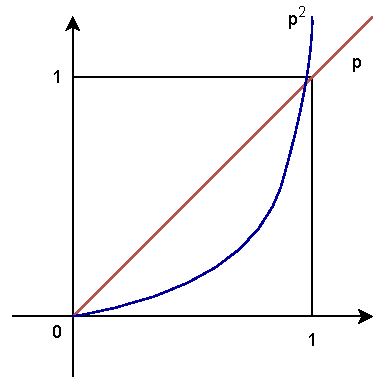
\includegraphics[scale = 0.8]{img/p.pdf}
\end{figure}
ma quindi, sempre approssimando (avendo quindi già due approssimazioni):
\[p[\mbox{ 1 errore }=n\cdot p\cdot(1-p)^{n-1}\simeq n\cdot p-n^2\cdot
  p^2+n\cdot p^2\simeq n\cdot p\]
Quindi:
\[p[\mbox{ 1 errore }\simeq n\cdot p\]
Analogamente ragiono per due errori:
\[p[\mbox{ 2 errori }]={{n}\choose{2}}\cdot
  p^2\cdot(1-p)^{n-2}\simeq{{n}\choose{2}}\cdot
  p^2\cdot[1-p\cdot(n-2)]={{n}\choose{2}}\cdot (p^2-n\cdot p^3+2p^3)\]
Ma anche qui si ha che $p\in(0,1)$ e quindi $p^3<p$, e quindi si ha:
\[p[\mbox{ 2 errori }]\simeq{{n}\choose{2}}\cdot p^2=\frac{n\cdot
    (n-1)}{2}\cdot p^2\]
In generale, per $k$ errori, con gli stessi passaggi:
\[p[\mbox{ k errori }]\simeq{{n}\choose{k}}\cdot p^k\]
\textbf{I conti diventano molto più semplici}.\\
Si è detto che se la probabilità di due errori è piccoli si può decidere di
trascurarla (usando poi solo il \textit{controllo di parità semplice}). Da
queste approssimazioni vediamo che la probabilità di un errori è $\simeq n\cdot
p$ mentre per due $\simeq\frac{n\cdot (n-1)}{2}\cdot p^2$. Se ipotizziamo $p\sim
10^{-6}$, quindi uno su un milione, si ha che $p^2=10^{-12}$ quindi assolutamente
trascurabile. Si segnala comunque che questa non è una pratica standard.
Normalmente si hanno, ad esempio, \textbf{low density parity codes (LDPC)} dove
si sparano a caso vari controlli di qualità nell'ottica di mantenere le
proprietà di correzione degli errori usando meno controlli possibile, avendo,
tornando alla ridondanza $R=1+\frac{check}{msg}$, che si vuole usare il minor
numero di cifre di controllo per abbassare l'\textit{eccesso di ridondanza},
abbassando la ridondanza stessa, avvicinandosi quindi a $1^+$ (ci si avvicina
da destra ovviamente). Riducendo l'\textit{eccesso di ridondanza} si ha che
ogni cifra di controllo \textit{copre/protegge} il maggior numero ci
simboli/cifre del messaggio. \textit{A parità di simboli inviati si vuole quindi
  ridurre il numero di cifre di controllo}.\\
Approfondiamo e usiamo quindi il\textit{ modello del rumore bianco} per vedere
qual è a probabilità che il ricevente non riesca a capire che c'è stato un
errore utilizzando il \textit{controllo di parità semplice}.\\
Ricordiamo che il messaggio è della forma:
\[x_1x_2\cdots x_{n-1}y\]
con $y$ \textit{controllo di parità semplice} calcolato come:
\[y=\bigoplus_{i=1}^{n-1}x_i\]
Un numero dispari di errore mi segnala che ci sono stati problemi, usando la
\textit{parità pari} (i pacchetti inseriti nel canale hanno un numero apri di
$1$).\\ 
Vogliamo quindi la probabilità che il controllo di parità fallisca, ovvero:
\[p[\mbox{ controllo }\bigoplus \mbox{ fallisce }]\]
ma questo è uguale alla probabilità che avvenga un numero pari di errori
(\textbf{zero escluso}, ovviamente):
{\footnotesize{\[p[\mbox{ controllo }\bigoplus \mbox{ fallisce }]=p[\mbox{ numero
      pari di errori }]=p[\mbox{ 2 errori }]+p[\mbox{ 4 errori }]+\cdots \]}}
Diciamo che, per comodità:
\[1=(1-p)+p=[(1-p)+p]^n\]
Ma so che $(a+b)^n=\sum_{k=0}^n{{n}\choose{k}}a^{n-k}b^k$, quindi:
\[1=[(1-p)+p]^n=\sum_{k=0}^n{{n}\choose{k}}(1-p)^{n-k}p^k\]
ma questa è ${{n}\choose{k}}(1-p)^{n-k}p^k=p[\mbox{ k errori }]$ (infatti la
somma di tutte le probabilità è appunto 1), quindi:
\[1=[(1-p)+p]^n=\sum_{k=0}^n{{n}\choose{k}}(1-p)^{n-k}p^k=\sum_{k=0}^np[\mbox{
    k errori }]\]
D'altro canto posso anche dire che, sempre applicando l'espansione di $(a+b)^n$,
scomponendo però $(-p)^k$ in $(-1)^k\cdot p^k$ (dove $(-1)^k$ vale $1$ per k
pari e $-1$ per $k$ dispari). Si ha quindi:
\[(1-2\cdot p)^n=[(1-p)-p]^n=\sum_{k=0}^n(-1)^k\cdot {{n}\choose{k}}\cdot
  p^k\cdot(1-p)^{n-k}\]
Ma quindi ho:
\[(1-2\cdot p)^n=
  \begin{cases}
    {{n}\choose{k}}\cdot  p^k\cdot(1-p)^{n-k} &\mbox{sse $k$ è pari}\\
    -{{n}\choose{k}}\cdot  p^k\cdot(1-p)^{n-k} &\mbox{sse $k$ è dispari}\\
  \end{cases}
\]
Quindi se $k$ è dispari le espansioni di $1$ e $(1-2\cdot p)^n$ sono uguali ma
di segno opposto mentre se $k$ è pari sono uguali con lo stesso segno. Ma quindi
questa somma delle due espansioni mi lascia col doppio dei soli termini con $k$
pari che ci aiuta volendo calcolare proprio le probabilità con un numero di
errori pari. Si ha quindi, dividendo già per due avendo il discorso del doppio:
\[\frac{1+(1-2\cdot p)^n}{2}=\sum_{t=0}^{\lfloor \frac{n}{2}\rfloor}
  {{n}\choose{2\cdot t}}\cdot p^{2t}\cdot(1-p)^{n-2t}\]
La somma va quindi da 0 alla parte intera di $\frac{n}{2}$. Nel coefficiente
binomiale ho $2\cdot r$ che è una quantità sicuramente pari. In generale è come
se avessi $k=2\cdot t$ ciclando solo sui $k$ pari. Ho quindi ottenuto:
\[p[\mbox{ 0 errori }]+p[\mbox{ 2 errori }]+p[\mbox{ 4 errori }]+\cdots \]
Non vogliamo però $t=0$ quindi:
{\footnotesize{\[p[\mbox{ controllo }\bigoplus \mbox{ fallisce }]=p[\mbox{
        numero pari di errori }]=\frac{1+(1-2\cdot 
    p)^n}{2}-p[\mbox{ 0 errori }]\]}}
\[=\frac{1+(1-2\cdot p)^n}{2}-  {{n}\choose{0}}\cdot
  p^{0}\cdot(1-p)^{n-0}=\frac{1+(1-2\cdot p)^n}{2}-(1-p)^n\]
E quindi:
{\small{\[p[\mbox{ controllo }\bigoplus \mbox{ fallisce }]=p[\mbox{ numero pari
        di errori }]=\frac{1+(1-2\cdot p)^n}{2}-(1-p)^n\]}}
D'altro canto potrei anche calcolare $p[\mbox{ numero dispari di errori }]$:
\[p[\mbox{ numero dispari di errori }]=1-p[\mbox{ numero pari di errori }]\]
(\textit{o anche modificando la sommatoria per ciclare sui $k$ dispari}).\\
Facendo qualche conto\footnote{i calcoli
  per il numero dispari di errore sono materiale extra sulle dispense del
  docente} si ottiene che: 
\[p[\mbox{ numero dispari di errori }]=1-(p[\mbox{ numero pari di errori
  }]+p[\mbox{ 0 errori }])\]
ovvero:
\[p[\mbox{ numero dispari di errori }]=\frac{1-(1-2\cdot p)^n}{2}\]
\textit{In generale il numero dispari di errori è meno interessante}.\\
\subsection{Gestione dei burst}
Come abbiamo introdotto con il solo \textit{controllo di parità} e con
il \textit{rumore bianco} non si possono gestire i \textbf{burst di
  errori}. Vediamo quindi un modo semplice per gestirli.\\
Si supponga di voler spedire dei messaggi formati da lettere, ad esempio:
\begin{table}[H]
  \centering
  \begin{tabular}{|c|c|c|c|}
    \hline
    c&i&a&o\\
    \hline
  \end{tabular}
\end{table}
Posiamo di rappresentare ogni lettera tramite l'\textbf{ASCII standard} a 7 bit:
\begin{table}[H]
  \centering
  \begin{tabular}{c|c}
    char & bit\\
    \hline
    c&1000011\\
    i&1001001\\
    a&1000001\\
    o&1001111
  \end{tabular}
\end{table}
Si supponga di avere dei burst di errori di lunghezza $L$ e per semplicità
assumo $L$ di lunghezza pari alle singole word, quindi $L=7$. Per gestire il
burst spedisco prima i 7 bit della prima lettera poi quelli della seconda
etc$\ldots$\\
Infine spedisco un intero pacchetto di bit di controllo di 7 bit dove ogni bit
viene calcolato controllando quella posizione di bit in tutti i pacchetti
precedenti, sempre tramite lo \textit{xor}. Nel caso d'esempio si ha quindi, con
$x$ per indicare il \textbf{check} (se nella colonna sopra ho un numero apri di
$1$ metto $0$ altrimenti $1$):
\begin{table}[H]
  \centering
  \begin{tabular}{c|c}
    c&1000011\\
    i&1001001\\
    a&1000001\\
    o&1001111\\
    \hline
    x&0000100\\
  \end{tabular}
\end{table}
Suppongo un burst che rovini dalla posizione 2 alla 4 incluse (avendo che quindi
molto probabilmente non ci torneranno i conti facendo il check su
$x[2,4]=000$).\\
Ovviamente anche qui un numero pari di errori inganna il sistema avendo comunque
un \textit{controllo di parità semplice} e anche in caso d'errore il ricevente
non sa comunque dove sia avvenuto e quindi fa \textbf{detection} ma non può fare
\textbf{correction}.
\subsection{Codici pesati}
Abbiamo già parlato del \textbf{codice 01247} vediamo ora un codice pesato più
interessante e utilizzato.\\
\begin{definizione}
  Definiamo questo \textbf{codice pesato} come un codice per cui si hanno alcune cifre
  di messaggio $msg=m_1m_2\cdots m_nc$ alle quali associamo dei pesi che
  dipendono dalla posizione in cui si trovano le varie cifre. In particolare si
  ha peso:
  \begin{itemize}
    \item $1$ per la \textbf{check digit} $c$
    \item $2$ per $m_n$
    \item si prosegue sempre aumentando di 1 per le altre cifre
    \item $n$ per $m_2$
    \item $n+1$ per $m_1$
  \end{itemize}
\end{definizione}
Questo si fa perché la cifra di controllo è calcolata per far ottenere:
\[m_1\cdot (n+1)+m_2\cdot n+\cdots+m_n\cdot 1+c\cdot 1=0\]
ma ovviamente questo non sembra possibile e infatti i conti sono fatti in
\textbf{modulo numero primo}, avendo per esempio, se scegliamo come numero
prima $37$:
\[m_1\cdot (n+1)+m_2\cdot n+\cdots+m_n\cdot 1+c\cdot 1\equiv 0\bmod\,\, 37\]
La scelta di 37 non è causale, infatti volendo:
\begin{itemize}
  \item rappresentare le 21 lettere dell'alfabeto inglese
  \item rappresentare dieci cifre da 0 a 9
  \item un simbolo per lo spazio
\end{itemize}
e quindi siamo a 32 simboli e ci serve un numero primo $\geq 31$ e quindi va
bene 37.\\
Vogliamo un numero prima perché se vogliamo fare i conti con le congruenze è
più semplice farle in \emph{modulo numero primo}.\\
Lavoriamo quindi nella classe dei resti:
\[[0]_{37},[1]_{37},\ldots, [36]_{37}\]
e in questo modo se facciamo le varie operazioni è tutto uguale al solito fino
a 36 (cosa che non succede per le classi dei resti in modulo non numero
primo).\\
La classe dei resti in modulo numero primo è un \textbf{campo} mentre se non
fosse primo si avrebbe un \textbf{anello}. In un campo se $x\cdot y=0$ o che
$x=0$ oppure $y=0$ (cosa che non succede negli anelli). Inoltre in un campo ho
che se $x\cdot y =z$ allora $x=z\cdot y^{-1}$ (in un anello non per tutti gli
$y$ esiste un $y^{-1}$ mentre in un campo sì).\\
Facendo dipendere il calcolo del peso della \textbf{check digit} da tutti gli
altri pesi perché, così facendo, sopratutto nelle comunicazioni di tipo
\textbf{seriale} (dove si spedisce una cifra alla volta), ci si accorge subito
se una cifra è andata persa oppure se si è aggiunta cifra o se due cifre si
sono scambiate (cosa comunque difficile in un sistema di comunicazione
elettronico ma è utile in altre situazioni, sopratutto di conti ``a
mano'').\\
Si supponga di avere delle cifre $b$ e $a$, la prima con peso $k+1$ e la
seconda con peso $k$, avendo una scrittura del tipo $cifra(peso)$:
\[b(k+1)+a(k)\]
Ipotizziamo di scambiare $a$ e $b$ (ora $a$ pesa $k+1$ e $b$ pesa $k$),
avendo:
\[a(k+1)+b(k)\]
Ma facendo la differenza si nota che non è nulla:
\[[b(k+1)+a(k)]-[a(k+1)+b(k)]\neq 0\]
infatti ho:
\[b\cdot k+b+a\cdot k-a\cdot k-a-b\cdot k=b-a\]
ma $b-a=0$ sse $b=a$ e quindi l'unico caso in cui non ci si accorge dello
scambio è avere lo scambio di due cifre uguali che non fa cambiare il
risultato.\\
Questa idea viene usata anche nei codici a barre. Vediamo quindi un algoritmo
per calcolare la cifra di controllo:
\begin{algorithm}[H]
  \begin{algorithmic}
    \Function{CheckCalc}{}
    \State $sum \gets 0$
    \State $ssum \gets 0$
    \While {\textit{not} EOF}
    \State \textbf{read} \textit{sym}
    \State $sum \gets sum+sym\,\,\, (\bmod\,\, 37)$
    \State $ssum \gets ssum+sum\,\,\, (\bmod\,\, 37)$
    \EndWhile
    \State $temp \gets ssum+sum\,\,\, (\bmod\,\, 37)$
    \State $c \gets 37-temp\,\,\, (\bmod\,\, 37)$
    \State \textbf{return} $c$ 
    \EndFunction
  \end{algorithmic}
  \caption{Algoritmo di calcolo dei pesi per codice pesato}
\end{algorithm}
Dove:
\begin{itemize}
  \item $sum$ tiene conto della somma numerica della nostro calcolo, accumulando
  i vari termini 
  \item $ssum$ che è una \textit{somma delle somme} e tiene conto implicitamente
  dei vari persi che crescono spostandoci da destra a sinistra come visto
  sopra. Si accumulano i termini e i loro pesi
\end{itemize}
\textit{I $\bmod 37$ nel ciclo sono in realtà superflui ma conviene farli per
  non far diventare i numeri troppo grossi. Le ultime due operazioni servono a
  risolvere alcune problematiche che non vediamo qui.}\\
Vediamo una più chiara simulazione.
\begin{esempio}
  Avendo, simulando per un messaggio $wxyzc$, con $c$ \textit{check digit}:
  \begin{table}[H]
    \centering
    \begin{tabular}{|c|c|c|}
      \hline
      msg & sum & ssum \\
      \hline
      $w$ & $w$ & $w$ \\
      $x$ & $w+x$ & $2\cdot w+x$ \\
      $y$ & $w+x+y$ & $3\cdot w+2\cdot x+y$ \\
      $z$ & $w+x+y+z$ & $4\cdot w+ 3\cdot x+2\cdot y+z$ \\
      \hline
      $c$ & $w+x+y+z+c$ & $5\cdot w+4\cdot x+3\cdot y+2\cdot z+c$ \\
      \hline
    \end{tabular}
  \end{table}
  Arrivato alla fine voglio calcolare $c$ in modo che:
  \[5\cdot w+4\cdot x+3\cdot y+2\cdot z+c \equiv 0 \bmod\,\, 37\]
\end{esempio}
Il mittente ha un messaggio e ci calcola la \textbf{check digit}.
Chi riceve fa lo stesso calcolo e alla fine controlla la \textbf{check
  digit}. Un altro modo per il ricevente è quello di fare solo l'ultimo calcolo
se farli tutti step by step.\\
Introduciamo un particolare tipo di codice, quello \textbf{ISBN
  (\textit{(International Standard BookNumber})} dei libri, che 
sono legati, per il codice a barre, allo standard europeo \textbf{EAN13} (negli
USA si usa lo standard 
\textbf{UPC}). In questo codice si hanno 10 cifre (con al più il carattere $X$)
che un identificano in modo univoco ad un libro. Nel dettaglio:
\begin{itemize}
  \item la prima cifra rappresenta lo stato in cui è stampato il libro. Questo
  ha problemi non avendo solo 9 stati che producono libri
  \item le successive 2 cifre sono le prime due per l'editore, anche questo è un
  problema in quanto alcuni stati hanno più di 100 case editrice
  \item le successive 6 sono il numero del libro
  \item l'ultima cifra è il checksum, la check digit
\end{itemize}
In realtà ho trattini dopo la prima cifra, dopo la quinta e dopo la nona ma non
contano nulla ai fini del calcolo ma sono aiutati solo per facilitare la
leggibilità dello stesso.\\
\textbf{A causa dei problemi sopra descritti i codici ISBN vengono assegnati
  ormai con libertà dalle case editrici, usando il primo codice libero}.\\
ISBN è un codice pesato dove i conti sono
fatti in $\bmod\,\,\,11$ (il più piccolo numero primo più grande di 10). Potrei
avere come risultato 10 avendo $\bmod\,\,\,11$ ma in quel caso uso $X$ come
checksum, come ultima cifra.
\begin{esempio}
  Prendiamo l'ISBN:
  \[0\mbox{-}1315\mbox{-}2447\mbox{-} x\]
  e vogliamo verificare che sia effettivamente $X$. Si ha (con $\equiv$ indico i
  conti $\bmod\,\,\,11$):
  \begin{table}[H]
    \centering
    \begin{tabular}{|c|c|c|}
      \hline
      msg & sum & ssum \\
      \hline
      0 & 0 & 0\\
      1 & 1 & 1\\
      3  & 4 & 5\\
      5 & 10 & $20\equiv 9$\\
      2& $12\equiv 1$ & $21\equiv 10$\\
      4 & 5 & $15\equiv 4$\\
      4 & 9 & $13\equiv 2$\\
      7 & $16\equiv 5$ & 7\\
      \hline
      $X\equiv 10$ & $15\equiv 4$ & $11\equiv 0$\\
      \hline
    \end{tabular}
  \end{table}
  Avendo che effettivamente la somma $\bmod\,\,\,11$ fa 0 e quindi è
  verificato.\\ 
  Avrei inoltre, per l'algoritmo, controllando la check digit:
  \[temp = 7+5=12\equiv 1\]
  \[c=11-1=10\equiv X\]
\end{esempio}
\section{Codici per correggere errori}
In questo caso il ricevente non solo deve capire dove è l'errore ma deve anche
correggerlo. 
\subsection{Codici rettangolari}
Il modo più semplice per correggere errori è usare i \textbf{codici a correzione
  rettangolari}. \\
In questo caso il codice viene organizzato in modo logico in forma di
rettangolo, ovviamente solo in modo logico/astratto.
Indichiamo con $\circ$ i bit di messaggio e con $x$ le check digit. In questa
prima soluzione penso ai codici come se fossero a forma di rettangolo, con $m-1$
righe e $n-1$ colonne, con extra una colonna di check digit e una riga extra di
check digit. Contando la riga di check digit e la colonna di check digit
arriviamo a $m$ righe e $n$ colonne.
\begin{table}[H]
  \centering
  \begin{tabular}{cccccc}
    $\circ$ & $\circ$ & $\circ$ &$\ldots$ & $\circ$ & x\\
    $\circ$ & $\circ$ & $\circ$ &$\ldots$ & $\circ$ & x\\
    $\circ$ & $\circ$ & $\circ$ &$\ldots$ & $\circ$ & x\\
    $\vdots$ & $\vdots$ & $\vdots$ &$\ddots$ & $\circ$ & x\\
    $\circ$ & $\circ$ & $\circ$ &$\ldots$ & $\circ$ & x\\
    x&x&x&x&x&(x)
  \end{tabular}
\end{table}
\textit{L'ultima check digit in fondo a destra è superflua, anche se a volte è
  lo xor di tutte le cifre di controllo, richiedendo che abbia numero pari di
  1}.\\ 
I codici rettangolari riescono a correggere un errore, uno e uno solo ma ovunque
avvenga.\\
La check digit della prima riga fa la parità della prima riga, analogamente la
seconda lo fa per la seconda riga etc$\ldots$\\
Faccio un discorso analogo sulle colonne (la colonna 1 ha la check digit come
prima cifra della riga di check digit etc$\ldots$).\\
La check digit mi dice sempre se ho cifre pari tra cifre di messaggio e check
digit.\\ 
Tramite la check digit a fine riga capisco che in una riga si ha un errore, e
posso controllare lo stesso per la colonna. Identifico quindi il punto preciso
in cui è avvenuto l'errore e semplicemente lo inverto, essendo binario.\\
Identificare l'errore singolo è dato dal fatto che solo una riga e solo una
colonna avranno la rispettiva check digit ``rotta'' (nella colonna di check
digit identifico la riga dell'errore mentre nella riga di check digit identifico
la colonna dell'errore) e quindi posso riconoscere il preciso elemento che è
errato. Da questo discorso si capisce che la check digit in fondo a destra è in
realtà inutile.\\ 
Ovviamente questo è garantito funzionare solo per un errore in quanto due errori
potrebbero avere in comune riga o colonna e non saprei più capire dove siano gli
errori. Potrebbe funzionare per più di un errore ma non sempre causa ambiguità e
quindi questo metodo è \textbf{garantito per uno e un solo errore, ovunque si
  trovi}.\\ 
Studiamo quindi la ridondanza, che ricordiamo essere in generale:
\[R=\frac{msg+check}{msg}=1+\frac{check}{msg}\]
Per il codice rettangolare si ha quindi:
\[R_{\sqsubset \! \sqsupset}=\frac{m\cdot n}{(n-1)\cdot
    (m-1)}=1+\frac{1}{m-1}+\frac{1}{n-1}+\frac{1}{(n-1)\cdot (m-1)}\]
Con quindi $\frac{1}{m-1}+\frac{1}{n-1}+\frac{1}{(n-1)\cdot (m-1)}$ che è il
nostro \textit{eccesso di ridondanza} e si ha che è $\geq 0$, quindi in
generale:
\[R_{\sqsubset \! \sqsupset}\geq 1\]
Ricordando che ``i bit non sono colorati'' potrei avere errori anche nelle
check digit. Supponendo però che si ha al massimo un errore e supponendo di non
avere, in quanto inutile, la check digit in basso a destra,  si ha che al più
trovo ``rotta'' o una riga (se ho errore un errore nella colonna di check digit)
o su una colonna (se ho errore un errore nella riga di check digit), capendo
così che ho ``rotta'' una check digit, sapendo anche quale.
\begin{esempio}
  Se devo spedire 24 bit posso rappresentarli in vari modi, secondo vari
  rettangoli (contando anche la check digit in basso a destra):  
  \begin{itemize}
    \item una riga per 24 colonne (più la riga di controllo), con quindi 26
    check digit
    \item 2 righe per 12 colonne (più la riga di controllo), con quindi 15
    check digit
    \item 3 righe per 8 colonne (più la riga di controllo), con quindi 12
    check digit
    \item 4 righe per 6 colonne (più la riga di controllo), con quindi 11
    check digit
    \item le simmetriche di quelle dette sopra
  \end{itemize}
  
\end{esempio}
Man mano che il numero di righe tende a quello di colonne (posto che, come
nell'esempio precedente, non sempre può diventare uguale) si ha che le cifre di
controllo diminuiscono. Tornando quindi alla formula della ridondanza vediamo
che al diminuire delle check digit diminuisce l'eccesso di ridondanza
$\frac{check}{msg}$ e quindi la ridondanza tende ad avvicinarsi a 1.
Quindi per scegliere $n$ e $m$ si cerca di fare si che siano il più uguali
possibili, avendo meno cifre di controllo.
Formalizzando quanto appena detto posso vedere la ridondanza la posso vedere
come una funzione: 
\[f(n,m)\]
avendo che $\frac{1}{m-1}+\frac{1}{n-1}+\frac{1}{(n-1)\cdot (m-1)}$ è quanto
fatto dalla funzione.
Si può quindi cercare il punto minimo di questa funzione trovando che è in
$m=n$.\\
Si può anche ipotizzare di poter aggiungere una cifra di messaggio per poter
avere una rappresentazione con $n=m$, ma ovviamente dipende da caso a
caso. Questo bit aggiuntivo a seconda del caso sarebbe 0 o 1. Si nota che
aumentare il messaggio aumenta $msg$ riducendo, a parità di check digit,
$\frac{check}{msg}$, aiutando ad arrivare ad una ridondanza prossima a
1. \textbf{Non sempre ho modo di aggiungere tale bit}.\\
Il caso migliore è quindi con $n=m$ e si ha quindi, avendo un quadrato, il
calcolo più preciso per la ridondanza:
\[R_\square=\frac{n^2}{(n-1)^2}=1+\frac{2}{(n-1)}+\frac{1}{(n-1)^2}\]
che è la ridondanza migliore che si può ottenere con i codici rettangolari.
\subsection{Codici triangolari}
Vediamo quindi i \textbf{codici a correzione triangolari}, dove la
rappresentazione è appunto triangolare (a occhio una sorta di matrice
triangolare).\\ 
In questo caso si ha un triangolo con un cateto di lunghezza $n$, ad esempio
(con $n=4$): 
\begin{table}[H]
  \centering
  \begin{tabular}{ccccc}
    $\circ$ & $\circ$ & $\circ$ &$\circ$  & x\\
    $\circ$ & $\circ$ & $\circ$  & x&\\
    $\circ$ & $\circ$ & x&&\\
    $\circ$ &x&&&\\
    x&&&&
  \end{tabular}
\end{table}
Ho quindi $n$ check digit (\textit{parte in dubbio}). Si ha infatti che le ci
cifre di messaggio sono (per la \textbf{formula di Gauss}):
\[msg=\sum_{i=1}^{n-1}i=\frac{(n-1)\cdot n}{2}\]
(in altre parole il numero di diagonali che ho nella matrice meno uno).\\
Ho inoltre che il numero di cifre totali è:
\[tot=msg+check=\frac{(n-1)\cdot n}{2}+n=\frac{n(n+1)}{2}\]
che altro non è che la sommatoria fatta per calcolare $msg$ ma con un'iterazione
in più:
\[tot=msg+check=\sum_{i=1}^{n}i\]
Le check digit vengono calcolate dal mittente in base alle cifre sulla riga e
sulla colonna della check digit. Quindi, ad esempio, per calcolare la check
digit in grassetto di:
\begin{table}[H]
  \centering
  \begin{tabular}{ccccc}
    $\circ$ & $\circ$ & $\circ$ &$\circ$  & x\\
    $\circ$ & $\circ$ & $\circ$  & x&\\
    $\circ$ & $\circ$ & \textbf{x}&&\\
    $\circ$ &x&&&\\
    x&&&&
  \end{tabular}
\end{table}
La calcola tramite le cifre di messaggio in verde:
\begin{table}[H]
  \centering
  \begin{tabular}{ccccc}
    $\circ$ & $\circ$ & ${\color{green}\circ}$ &$\circ$  & x\\
    $\circ$ & $\circ$ & ${\color{green}\circ}$  & x&\\
    ${\color{green}\circ}$ & ${\color{green}\circ}$ & \textbf{x}&&\\
    $\circ$ &x&&&\\
    x&&&&
  \end{tabular}
\end{table}
Si nota che il bit di parità della prima riga è calcolato solo tramite la prima
riga mentre il bit di parità dell'ultima riga viene calcolato solo tramite la
prima colonna.\\
Il ricevente, per capire dove è il bit errato, verifica in quali check digit è
coinvolto, che sono due check digit, e incrociando scopro quale sia il simbolo
errato. Vedendo in pratica si supponga errato il bit in rosso:
\begin{table}[H]
  \centering
  \begin{tabular}{ccccc}
    $\circ$ & $\circ$ & $\circ$ &$\circ$  & x\\
    $\circ$ & $\circ$ & {$\color{red}\circ$}  & x&\\
    $\circ$ & $\circ$ & x&&\\
    $\circ$ &x&&&\\
    x&&&&
  \end{tabular}
\end{table}
Esso è coinvolto nelle seguenti cifre di parità in grassetto, calcolate, oltre
che grazie alla cifra in rosso anche da quelle in verde:
\begin{table}[H]
  \centering
  \begin{tabular}{ccccc}
    $\circ$ & $\circ$ &  ${\color{green}\circ}$&  ${\color{green}\circ}$ & x\\
    ${\color{green}\circ}$ & ${\color{green}\circ}$ & {$\color{red}\circ$}  & \textbf{x}&\\
    ${\color{green}\circ}$ &  ${\color{green}\circ}$ & \textbf{x}&&\\
    $\circ$ &x&&&\\
    x&&&&
  \end{tabular}
\end{table}
Mentre le altre cifre di parità saranno corrette. Il destinatario può quindi
scoprire quale sia il bit che è stato modificato per poterlo poi correggere.\\
Passiamo quindi alla ridondanza del codice triangolare.
Si ha che:
\[R_\triangle=\frac{tot}{msg}=\frac{\frac{n(n+1)}{2}}{\frac{(n-1)n}{2}}=
  \frac{n+1}{n-1}= \frac{(n-1+2)}{n-1}=1+\frac{2}{n-1}\]
Confronto questa ridondanza con quella dei migliori codici rettangolari, ovvero
quella dei codici quadrati, dove vedo che si ha un termine positivo in più nei
codici quadrati, ovvero $\frac{1}{(n-1)^2}$, che essendo positivo può solo
aumentare la ridondanza. Si ha quindi che:
\[R_\triangle<R_\square\]
e quindi i codici triangolari sono migliori di quelli
rettangolari, anche dei migliori tra quelli rettangolari (quelli quadrati), e
hanno una sola check digit per riga e una sola per colonna.\\
L'unico limite per avere un codice triangolare è quello di avere un
messaggio di $n$ cifre che permette l'espressione $\frac{(n-1)\cdot n}{2}$,
ovvero che sia rappresentabile da un triangolo (per fare tornare i conti posso
comunque aggiungere uno 0, per esempio), avendo $n$ lunghezza del cateto. 
\subsection{Codici cubici}
Per cercare di abbassare ancora meno la ridondanza cerchiamo la disposizione
geometrica più conveniente. Si è provato quindi ad aumentare le dimensioni dello
spazio in cui ci troviamo, pensando ad un cubo, ipotizzando di avere una cifra
di controllo (posta in basso a destra per il piano) che controlla tutto un piano
(contando che ho piani per ognuna delle tre dimensioni). Si ha quindi un bit di
parità per ogni piano (che è ciò che rappresenta le cifre di messaggio) con cui
posso tagliare il cubo. Nel complesso si ha quindi un intero spigolo del cubo
che rappresenta le check digit che sono rappresentati da i piani in una
certa direzione. In totale posso sezionare in tre direzioni avendo quindi 3
spigoli di check digit che ``proteggono'' tutte le cifre di messaggio
contenute nel cubo (che ha lato $n-1$ più la check digit).\\
\begin{table}
  \centering
  \begin{tabular}{|c|cc|cc|cc|}
    \hline & \multicolumn{2}{|c|}
             { Quadrato } & \multicolumn{2}{c|}
                            { Triangolare } & \multicolumn{2}{c|} { Cubico } \\
    \hline&messaggio&controllo& messaggio&controllo & messaggio &controllo \\
    $n$ & $(n-1)^{2}$ & $2 n-1$ & $\frac{n(n-1)}{2}$&$n$&$n^{3}-3 n+2$&$3 n-2$ \\
    \hline 2 & 1 & 3 & 1 & 2 & 4 & 4 \\
    3 & 4 & 5 & 3 & 3 & 20 & 7 \\
    4 & 9 & 7 & 6 & 4 & 54 & 10 \\
    5 & 16 & 9 & 10 & 5 & 112 & 13 \\
    6 & 25 & 11 & 15 & 6 & 200 & 16 \\
    7 & 36 & 13 & 21 & 7 & 324 & 19 \\
    8 & 49 & 15 & 28 & 8 & 490 & 22 \\
    9 & 64 & 17 & 36 & 9 & 704 & 25 \\
    10 & 81 & 19 & 45 & 10 & 972 & 28 \\
    \hline
  \end{tabular}
  \caption{Esempio di tabella di confronto tra codici quadrati, triangolari e
    cubici} 
\end{table}
In maniera approssimata, su circa $n^3$ posizioni si hanno $3(n-1)+1=3n-2$ check
digit. Si ha quindi che la ridondanza è:
\[R_{\mbox{\mancube}}=\frac{(n-1)^3+3n-2}{(n-1)^3}=1+\frac{3n-2}{(n-1)^3}
  \simeq 1+\frac{3}{n^2}\]
Posso pensare quindi pensare di aumentare ancora le dimensioni, considerando
cubi a quattro dimensioni (e non mi serve disegnarlo visto che devo solo
``pensarlo''), avendo: 
\begin{itemize}
  \item $(n-1)^4$ cifre di messaggio 
  \item $4(n-1)+1=4n-3$ check digit
\end{itemize}
ottenendo la seguente ridondanza:
\[R_{\mbox{\mancube  \textit{4-dim}}}=1+\frac{4n-3}{(n-1)^4}\simeq
  1+\frac{4}{n^3}\]
(\textit{dove praticamente si è ignorato il $-3$ nella formula della check
  digit}).\\ 
Posso pensare di andare quindi in $k$ dimensioni, avendo:
\begin{itemize}
  \item $(n-1)^k$ cifre di messaggio 
  \item $k(n-1)+1=kn-k+1$ check digit
\end{itemize}
ottenendo la seguente ridondanza, con $k$ che è fissato e quindi costante:
\[R_{\mbox{\mancube  \textit{k-dim}}}=1+\frac{kn-k+1}{(n-1)^k}\simeq
  1+\frac{k}{n^{k-1}}\]
Possiamo così, facendo crescere $k$ e l'eccesso di ridondanza, ottenere una
figura sempre migliore.\\
Ma anche se la ridondanza è sempre migliore vedo che a denominatore dell'eccesso
di ridondanza $\frac{k}{n^{k-1}}$ trovo un polinomio elevato alla dimensione
meno uno. Vedremo che nei \textbf{codici di Hamming}, per correggere un errore,
il \textit{gap} è esponenziale al variare delle dimensioni. Inoltre il
\textit{codice di Hamming} è \textbf{ottimale}.
\subsection{Codici di Hamming}
Hamming si pone di trovare un codice per correggere un errore nel modello del
rumore bianco, avendo che sia però un \textbf{codice ottimale}, \textit{ovvero
  che a parità di cifre inviate deve usare il minimo numero di check digit}.
Ho sempre un pacchetto di $n$ bit che sono di due tipi:
\begin{enumerate}
  \item $k$ bit di cifre di messaggio $msg$
  \item $m$ bit di check digit $check$
\end{enumerate}
Per calcolare le check digit usa delle equazioni di controlli di parità, con una
cifra di messaggio che nel complesso serve a calcolare più di una check digit
(come nei codici legati alle figure numeriche). Si avranno quindi $m$ equazioni
di parità del tipo, avendo $c_1,\ldots,c_n$ cifre di parità e $x_i,\cdots x_n$
cifre di messaggio:
\[c_i=x_j\oplus x_k\oplus x_w \cdots\]
Tutte queste equazioni devono essere \textbf{linearmente indipendenti}, in modo
che ogni check digit abbia informazioni differenti. Supponiamo infatti:
\[c_1=x_1\oplus x_2\oplus x_5 \oplus x_7\]
\[c_2=x_5\oplus x_7\oplus x_8 \oplus x_9\]
Ma in realtà $c_i$ è una della $x_j$ della formula infatti:
\[c_1\oplus x_1\oplus x_2\oplus x_5 \oplus x_7=0\]
e quindi:
\[x_1\oplus x_2\oplus x_5 \oplus x_7=c_1\]
Scriviamo quindi:
\[c_1\to x_1\oplus x_2\oplus x_5 \oplus x_7=0\]
\[c_2\to x_5\oplus x_7\oplus x_8 \oplus x_9=0\]
In generale le equazioni mi danno 0 se il numero di 1 è pari.\\
\textbf{In ogni formula si assume di avere una sola cifra di messaggio.}\\
Faccio poi lo $\oplus$ tra $c_1$ e $c_2$ bit a bit, ottenendo (avendo tipo $x_5$
da entrambe le parti si semplifica):
\[c\to x_1\oplus x_2\oplus x_8\oplus x_9=0\]
Si supponga ora di avere una $c_3=c$ ma avrei uno spreco di fatica in quanto le
informazioni delle prime due sarebbero uguali alla terza, avendo infatti
\textit{dipendenza lineare}.\\
Ricordiamo che:
\[a_1\vec{v_1}+a_2\vec{v_2},a_1,a_2\in \mathbb{R}, \vec{v_1},\vec{v_2}\in
  \mathbb{R}^n\]
con $\mathbb{R}^n$ che è uno \textbf{spazio vettoriale}.\\
Fare \textbf{combinazioni lineari} in questo caso prevede la somma come il
$\oplus$. Rappresento le equazioni di parità dell'esempio sopra come un vettore
di $\{0,1\}^n$:
\[(1,1,0,0,1,0,1,0,0)\]
\[(0,0,0,0,1,0,1,1,1)\]
e facendo lo \textit{xor} (che è la somma $\bmod,\,\,\,2$ bit a bit) ottengo:
\[(1,1,0,0,0,0,0,1,1)\]
Si ha ora il prodotto scalare in $\{0,1\}^n$:
\[0\cdot \vec{v}=\vec{0}\]
\[1\cdot \vec{v}=\vec{v}\]
Quindi nel nostro caso:
\[a_1\vec{v_1}+a_2\vec{v_2},a_1,a_2\in \{0,1\}, \vec{v_1},\vec{v_2}\in
  \{0,1\}^n\]
Quindi 0 mi dice di non considerare il vettore e uno di considerarlo, indicando
il sottoinsieme di elementi da sommare.
Si ha che $\{0,1\}^n$ rispetto alla somma come definita e al prodotto scalare
come definito è uno \textbf{spazio vettoriale}.\\
Quindi, tornando a Hamming, possiamo capire, grazie a questi ragionamenti,
l'indipendenza lineare tra le equazioni di parità. Con $m$ bit di controllo si
cerca di capire quante condizioni d'errore si riesce a rappresentare. Con $m$
cifre di controllo si hanno $2^m$ possibili combinazioni/configurazioni. Ogni
configurazione mi deve identificare un errore diverso per poter fare anche
correzione. Mi serve però anche una configurazione che indichi il \textit{non
  avere errori}. Si ha quindi che si hanno:
\begin{itemize}
  \item $2^m-1$ condizioni di errore
  \item una condizione di non errore
\end{itemize}
Gli errori possono avvenire ovunque, anche nelle check digit, ma con al massimo
un errore (o nella prima posizione o nella seconda etc$\ldots$). SI hanno quindi
$n$ possibili condizioni d'errore. Si ha quindi che:
\[2^m\geq n+1\]
ovvero le configurazioni che posso fare con $m$ cifre di controllo deve
indicarmi le $n$ possibili condizioni d'errore più una per l'assenza di errore.
Nel caso dei codici di Hamming ``propriamente detti'' si avrebbe:
\[2^m= n+1\]
usando tutte le combinazioni in quanto il $>$ implicherebbe che sto
``sprecando'' qualche configurazione delle cifre di controllo. \textbf{Non
  sempre posso usare ``=''}.\\
Posso quindi capire quante siano le cifre di controllo.
\begin{esempio}
  Si supponga di voler spedire $k=4$ cifre di messaggio. Ci chiediamo di
  calcolare $m$:
  \[2^m\geq n+1\]
  ma quindi, avendo $n=m+k$:
  \[2^m\geq m+k+1\]
  Mi serve quindi l'$m$ più piccolo possibile che risolva la disequazione con
  $k=5$: 
  \[2^m\geq m+5\]
  Non si ha però una soluzione analitica ma $2^m$ cresce più velocemente di
  $m+5$ ($m=0$ non ha senso ma lo si mette, si hanno comunque tecniche anche per
  non partire da 1):
  \begin{table}[H]
    \centering
    \begin{tabular}{c||c|c}
      $m$& $2^m$ & $m+5$\\
      \hline
      \hline
      0 & 1 & 5\\
      1 & 2 & 6\\
      2 & 4 & 7\\
      3 & 8 & 8
    \end{tabular}
  \end{table}
  quindi $m=3$ è il più piccolo valore che risolve, risolvendo per di più con
  $=$ e non $\geq$. Per 4 bit di messaggio mi servono 3 cifre di controllo. Ho
  quindi $n=7$.
\end{esempio}
In generale per correggere un errore devo sapere in che posizione è, sapendo
l'indice da 1 a $n$ indicante tale posizione nel pacchetto. Il metodo che lo
calcola può restituire 0, indicante che non si ha errore.\\
Faccio una tabella con posizione/binario, ad esempio per l'esempio precedente
\begin{table}[H]
  \centering
  \begin{tabular}{c|c}
    pos& bin \\
    \hline     
    1 & 001\\
    2 & 010\\
    3 &011\\
    4&100\\
    5&101\\
    6&110\\
    7&111\\
    \hline
    \hline
    &   $c_3c_2c_1$
  \end{tabular}
\end{table}
Ho che i bit hanno $m$ cifre, e ho $c_3c_2c_1$ (si parte da destra) come le
cifre di parità ottenute dalle tre colonne di binari.\\
Ipotizzo un errore in posizione 5. Ho che, mettendo le $x_i$ dove si ha 1:
\[c_1\to x_1\oplus x_3\oplus x_5 \oplus x_7=0\]
ma ho problemi con $x_5$, avendo l'equazione pari a 1.\\
\[c_2\to x_2\oplus x_3\oplus x_6 \oplus x_7=0\]
dove non ho problemi con $x_5$.\\
\[c_3\to x_4\oplus x_5\oplus x_6 \oplus x_7=0\]
ma ho problemi con $x_5$, avendo l'equazione pari a 1.\\
Si ha quindi che:
\[c_1\to x_1\oplus x_3\oplus x_5 \oplus x_7=1\]
\[c_2\to x_2\oplus x_3\oplus x_6 \oplus x_7=0\]
\[c_3\to x_4\oplus x_5\oplus x_6 \oplus x_7=1\]
Che quindi mi mostra dopo l'uguale la posizione in cui è avvenuto
l'errore. I bit letti dal basso verso l'alto sono $101$ e questo è detto
\textbf{sindrome}, che quindi nei codici di Hamming è la 
posizione dell'errore in codice binario. \\
Se la \textit{sindrome} è 0 non ho errori (è come se avessi 000 nella prima riga
della tabella).\\
Il ricevente è sistemato ma manca il mittente che deve calcolare gli $m$ bit di
controllo e spedire. Usando la tecnica di usare nelle equazioni le $x_i$
relative agli 1 mi genera equazioni linearmente indipendenti. \\
Manca capire dove
mettere la check digit. Le cifre di controllo vengono messe nelle posizioni in
cui si ha un 1 solo, ovvero 001, 010 e 100, in modo che $c_1$ è solo nella prima
equazione, $c_2$ nella seconda e $c_3$ nella terza, non dovendo risolvere in
realtà il sistema lineare. Si quindi, nell'esempio sopra:
\[c_1\oplus x_3\oplus x_5 \oplus x_7=0\]
\[c_2\oplus x_3\oplus x_6 \oplus x_7=0\]
\[c_3\oplus x_5\oplus x_6 \oplus x_7=0\]
ottenendo quindi il pacchetto.
\[pacchetto = c_1c_2m_1c_3m_2m_3m_4\]
e quindi:
\[c_1\oplus m_1\oplus m_2 \oplus m_4=0\]
\[c_2\oplus m_1\oplus m_3 \oplus m_4=0\]
\[c_3\oplus m_2\oplus m_3 \oplus m_4=0\]
ma isolando le $c_i$, sommando da entrambe le parti dell'equazione:
\[c_1= m_1\oplus m_2 \oplus m_4\]
\[c_2= m_1\oplus m_3 \oplus m_4\]
\[c_3= m_2\oplus m_3 \oplus m_4\]
\textbf{Si noti che le posizioni delle cifre di controllo $c_i$ sono potenze di
  2 $2^0,2^1,2^2,\ldots$} e all'aumentare delle cifre della grandezza si ha
crescita logaritmica delle check digit, che quindi controllano un numero
esponenziale di cifre di messaggio.\\
\begin{esempio}
  Scelgo un messaggio di 4 bit:
  \[msg=1011\]
  quindi:
  \[pacchetto=c_1c_21c_3011\]
  So che, per le formule sopra (ma lo posso vedere anche col discorso di avere
  periodicità nella tabella di bit, pensando a come li scrivi quando fai le
  tabelle di verità):
  \[c_1=0\]
  \[c_2=1\]
  \[c_3=0\]
  quindi:
  \[pacchetto=0110011\]
  che viene inviato ma al destinatario arriva:
  \[pacchetto=0110111\]
  quindi con il bit in $i=5$ errato. Si rifanno i conti e si ottiene, calcolando
  la sindrome:
  \[s_1=1\]
  verificata vedendo i bit dispari.
  \[s_2=0\]
  verificata vedendo a coppie alternate ma saltando il primo bit (che sarebbe la
  coppia di 0 se avessi 000 in cima alla tabella, torna quindi comodo partire
  dal fondo della tabella per fare questi ragionamenti).
  \[s_3=1\]
  verificata vedendo gli ultimi 4 bit.\\
  Avendo sindrome $s=s_3s_2s_1=101$ che indica proprio la posizione 5.\\
  Vediamo invece se arriva:
  \[pacchetto=0010011\]
  quindi con il bit in $i=2$ errato (e sarebbe una check digit). Si ha che:
  \[s_1=0\]
  \[s_2=1\]
  \[s_3=0\]
  Avendo sindrome $s=s_3s_2s_1=010$ che indica proprio la posizione 2.\\
  Supponiamo ora che arrivi senza errori:
  \[pacchetto=0110011\]
  Si ha:
  \[s_1=0\]
  \[s_2=0\]
  \[s_3=0\]
\end{esempio}
\textit{I pacchetti di 7 bit che producono sindrome nulla sono quindi
  $2^{4}=16$, avendo che posso fare $2^4$ modi diversi di avere i 4 bit di
  messaggio ma ciascuno ha una sola tripla, 000, di check digit che mi dice che
  il pacchetto è valido}. Generalizzeremo poi questa cosa, ovvero che si hanno:
\begin{itemize}
  \item $n$ bit di pacchetto 
  \item $\log_2 n$ check digit
  \item $n-\log_2 n$ cifre di messaggio
  \item $2^{n-\log_2 n}$ combinazioni possibili delle cifre di messaggio per avere
  un pacchetto senza errori
\end{itemize}
Avere due errori rende impossibile capire dove siano, rendendo impossibile la
correzione.
\begin{esempio}
  Riprendendo l'esempio sopra si ipotizzi arrivi:
  \[pacchetto=0010111\]
  con errori in 2 e 5.\\
  Si ha per la sindrome:
  \[s_1=1\]
  \[s_2=1\]
  \[s_3=1\]
  Si avrebbe posizione in $111$ ovvero 7 (e non è un caso sia 5+2 ma la cosa non
  ci aiuterebbe a capire dove sia l'errore), a riprova
  che non si riesce ad identificare due errori. Non solo, si identifica un posto
  corretto come errato e lo corregge, introducendo un ulteriore errore.
\end{esempio}
La probabilità di avere due errori è comunque a $\frac{1}{2^{4096}}$ e quindi è
0, ``è la stessa probabilità che un tornado assembli i pezzi sparsi di un aereo
al punto di farlo funzionare''.\\
I codici di Hamming con $=$ e non $\geq$ sono quelli tali per cui:
\[n=2^m-1\]
\textbf{Sul file di esercizi nella pagina del corso esempio con $m=4$ a
  \textit{pagina 12}, \textit{potrebbe esserci un errore di conto sulla
    ridondanza}. Guardare anche per spunti teorici}.\\ 
Studiamo anche la ridondanza. Ricordando $2^m\geq n+1$ e nei codici ``migliori''
$2^m=n+1$ possiamo dire $2^m\simeq n$ e quindi $m\simeq \log_2 n$ (e con questo
$m$ posso riscrivere $k= n-\log_2n$). Ne segue che:
\[R=1+\frac{check}{msg}=1+\frac{m}{k}=1+\frac{\log_2 n}{n-\log_2n}\simeq
  1+\frac{\log_2n}{n}\]
(\textit{facendo un'approssimazione molto ``spinta''}).\\
\textbf{Sul file di esercizi nella pagina del corso esempio con $m=2$ a pagina
  13, occhio che non è $\frac{2}{3}$ ma $\frac{2}{1}$ nella ridondanza. Guardare
  anche per spunti teorici (manca la parte di esercizio in se calcolando la
  sindrome)}.\\ 
Vediamo quindi l'interpretazione geometrica del codice di Hamming, ricordando
che $n$ bit entrano nel canale ed escono $n$ bit $\in \{0,1\}^n$. Il messaggio
$M$ è quindi $M\subseteq \{0,1\}$. Cerchiamo di capire come assegnare che un
messaggio sia valido o meno.\\
Posso vedere $\{0,1\}^n$ come uno \textbf{spazio vettoriale} dove i vettori sono
$\vec{x}=(x_1,x_2,\ldots,x_n), \forall x_i\in\{0,1\}$ ovvero
$x_i\in\mathbb{Z}_2$. Due vettori in questo spazio, per definizione di spazio
vettoriale, possono essere sommati. Preso 
anche $\vec{x}=(y_1,y_2,\ldots,y_n), \forall y_i\in\{0,1\}$ la somma altro non
è che lo \textit{xor} componente per componente $\vec{x}+\vec{y}=(x_1\oplus y_1,
x_2\oplus y_2,\ldots)$. \\
Preso uno scalare $a\in \mathbb{Z}_2$ ho che $a\vec{x}=(ax_1,ax_2\ldots)$ con il
prodotto scalare che è praticamente l'\textit{and}. Si ha che:
\[a\vec{x}=
  \begin{cases}
    \vec{0} &\mbox{se } a=0\\
    \vec{x} &\mbox{se } a=1
  \end{cases}
\]
Vediamo i messaggi come \textbf{vertici di un n-cubo} ma non tutti i messaggi
sono validi. Ci serve un modo per capire quali sono validi per rendere difficile
che un errore mi porti da un messaggio valido ad un altro.
\begin{definizione}
  Definiamo \textbf{distanza di Hamming} come il numero di posizioni in cui due
  vettori $\vec{x}$, $\vec{y}$ differiscono, cioè per cui $x_1\neq y_i$. Questa
  è una vera e propria distanza in $\{0,1\}^n$. Tale distanza si indica con:
  \[d(\vec{x},\vec{y})\]
  con:
  \[d:\{0,1\}^n\times\{0,1\}^n\to\mathbb{R}\]
  Si hanno tre proprietà:
  \begin{itemize}
    \item $d(\vec{x},\vec{y})$ sse $\vec{x}=\vec{y}$
    \item $d(\vec{x},\vec{y})=d(\vec{y},\vec{x})$
    \item $d(\vec{x},\vec{z})\leq(\vec{x},\vec{y})+d(\vec{y},\vec{z})$,
    \textbf{diseguaglianza triangolare}
  \end{itemize}
  e quindi la \textbf{distanza di Hamming} è una \textbf{metrica} per lo spazio
  $\{0,1\}^n$.\\
  Spesso $d(\vec{x},\vec{y})$ si indica con $d_h(\vec{x},\vec{y})$.
\end{definizione}
\begin{definizione}
  Definiamo \textbf{peso di Hamming} come il numero di bit uguali a 1 e lo si
  indica con:
  \[w_j(\vec{x})\]
  Avendo che:
  \[w_j(\vec{x})=\sum_{i=1}^n x_1=d_h(\vec{x},\vec{0})\]
\end{definizione}
\begin{esempio}
  Prendiamo $n=3$. \\
  Disegnano supponiamo di avere qualcosa del tipo:
  \begin{figure}[H]
    \centering
    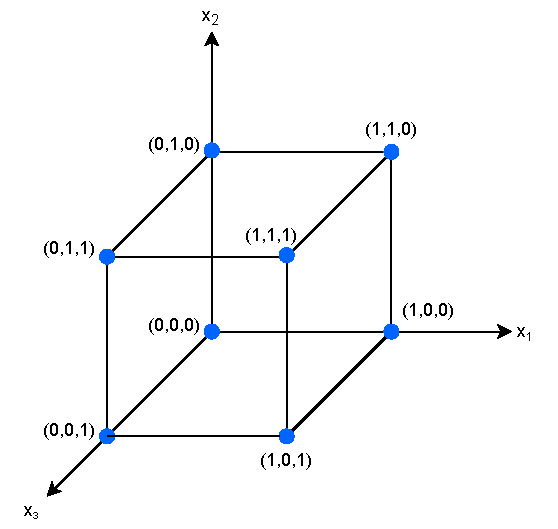
\includegraphics[scale = 0.8]{img/cubeh.pdf}
  \end{figure}
  Prendo i vertici $(x_1,x_2,x_3$):
  \begin{itemize}
    \item $(0,0,0)$
    \item $(1,0,0)$
    \item $(0,1,0)$
    \item $(0,0,1)$
    \item $(1,1,0)$
    \item $(0,1,1)$
    \item $(1,0,1)$
    \item $(1,1,1)$
  \end{itemize}
  \textit{Questi sono i nostri messaggi}.\\
  \textbf{Oltre $n=3$ farei lo stesso ma non saprei disegnarlo, avrei $n$
    lati che partono dall'origine appoggiati agli $n$ assi}.\\
  Suppongo di spedire $010$ e che si abbia un errore che porti a $110$ e sul
  cubo si nota che ci ha fatto spostare lungo un lato. \\
  Suppongo che da $010$ si arrivi a $100$, con due errori, si nota che ho due
  lati visitati sul cubo.\\
  Scegliamo quindi come messaggi validi punti che sono abbastanza distanti tra
  loro. Sicuramente quelli che si ottengono con un solo cambiamento non sono
  validi, parto quindi dal messaggio valido e impongo che tutti quelli che sono
  a \textbf{distanza 1} (parlando di \textbf{distanza di Hamming}) sul cubo,
  ovvero tutti quelli che raggiungo con un solo lato, non siano validi.\\
  \textbf{Essendo in $\{0,1\}^n$ in realtà esistono solo i vertici del cubo, i
    lati servono solo per capire meglio.}
\end{esempio}
Generalizziamo meglio.\\
Se ho la distanza di Hamming e varie caratteristiche del codice ho che:
\begin{itemize}
  \item se ho due codeword valide che hanno distanza 1 allora il codice ha
  capacità di \textbf{0 detection e 0 correction} in quanto potrei passare con
  un solo errore ad un messaggio valido
  \item se ho due codeword valide che hanno distanza 2 (e non esistono due
  codeword valide con distanza minore di 2) allora il codice ha
  capacità di \textbf{1 detection e 0 correction} in potrei avere più codeword
  valide a distanza di 1 da quella errata e quindi non saprei come fare
  correzione, non sapendo dove si trovi il bit errato. In ogni caso un errore
  viene sempre riconosciuto, anche se non può essere corretto. Se ho due errori
  potrei finire nuovamente in una codeword valida ma si sta assumendo che avendo
  scelto questo codice si sappia che la probabilità che avvengano due errori sia
  pressoché nulla. Il\textit{ controllo di parità semplice} è di questo
  tipologia.
  \newpage
  Graficamente avrei 
  una cosa del tipo, avendo in blu le codeword valide e in rosso quelle non
  valide: 
  \begin{figure}[H]
    \centering
    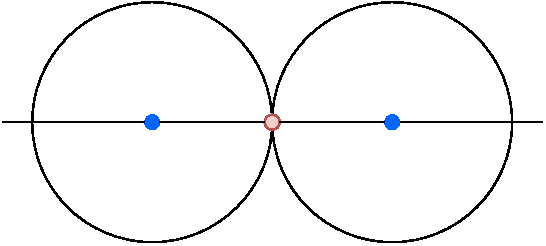
\includegraphics[scale = 0.8]{img/circ2.pdf}
  \end{figure}
  Notando come non sarei in grado di capire a che codeword valida ricondurmi.
  \item se ho due codeword valide che hanno distanza 3 (e non esistono due
  codeword valide con distanza minore di 3) allora il codice ha
  capacità di \textbf{2 detection e 1 correction}, riuscendo a correggere un
  errore. Se avessi due errori riconoscerei come codeword valida una a distanza
  1 da quella errata che però non è quella giusta, introducendo un nuovo
  errore. I \textit{codici di Hamming} sono di questo tipo. Graficamente avrei
  una cosa del tipo, avendo in blu le codeword valide e in rosso quelle non
  valide: 
  \begin{figure}[H]
    \centering
    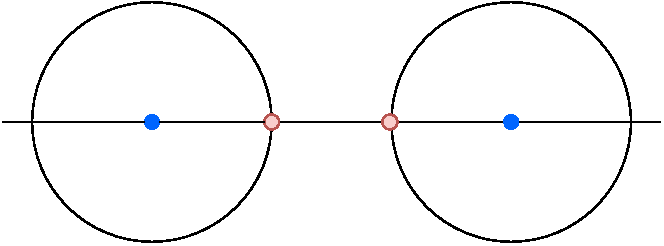
\includegraphics[scale = 0.8]{img/circ3.pdf}
  \end{figure}
  Notando che con un solo errore sarei in grado di capire a che codeword
  ricondurmi 
  \item se ho due codeword valide che hanno distanza 4 (e non esistono due
  codeword valide con distanza minore di 4) allora il codice ha
  capacità di \textbf{3 detection e 1 correction}, riuscendo a correggere un
  errore. Se avessi due errori riconoscerei avrei più codeword valide alla
  stessa distanza. Se avessi tre errori varrebbe quanto detto nel caso di
  distanza 2
   \item se ho due codeword valide che hanno distanza 5 (e non esistono due
  codeword valide con distanza minore di 5) allora il codice ha
  capacità di \textbf{4 detection e 2 correction}, per gli stessi discorsi fatti
  avendo distanza 3
\end{itemize}
Si nota quindi che al crescere della distanza di Hamming minima tra due codeword
cresce la capacità di detection e correction.\\
Possiamo ipotizzare che la codeword valida venga avvolta da una sfera di raggio
pari a $r$ avendo che $r$ sia tale per cui le sfere di due codeword valide non
si sovrappongano. Possiamo notare che in base alle osservazioni fatte sopra $r$
è il valore della capacità di detection. \\
Una sfera centrata nel punto $\vec{x}$ di raggio $r$ è l'insieme dei punti
$\vec{y}\in\{0,1\}^n$ tale che la distanza da $\vec{x}$ è minore di $r$, ovvero:
\[S(\vec{x},r)=\{\vec{y}\in\{0,1\}^n|\,d_h(\vec{x},\vec{y})\leq r\}\]
\textbf{Si noti che in $\{0,1\}^n$ somma e sottrazione bit a bit portano allo
  stesso risultato. }\\
Possiamo dire che:
\[output=input+errore\]
dove $errore$ è un vettore rappresentante l'errore (avendo $1$ dove ho
l'errore). Quindi:
\[errore = output -input\]
\begin{esempio}
  Tornando all'esempio sopra ipotizzo entri $011$ ed esca $111$, avendo quindi
  $d_h=1$. \\
  Sommo i due vettori:
  \[011\oplus 111=100\]
  Avendo che $100$ è l'errore.
\end{esempio}
\begin{esempio}
  Si vuole costruire un codice che consenta di correggere un errore, per poi
  confrontarlo con il codice di Hamming.\\
  Ci servono quindi codeword valide ad almeno distanza 3, prendendo messaggi
  validi e circondarli di sfere di raggio 1 tali che non si abbiano
  sovrapposizioni con altre sfere.\\
  Si ha $\{0,1\}^n$ come spazio vettoriale dove si hanno $2^n$
  elementi/vettori. \\
  In generale se prendo il volume dello spazio e lo divido per il volume di una
  sfera ho il numero di sfere che posso metterci:
  \[\frac{V_{spazio}}{V_{sfera}}\geq \mbox{numero massimo di sfere}\]
  Pongo $k$ uguale al numero di bit dei messaggi validi (non pari a $n$ ma
  prendo quindi una porzione di messaggio rappresentante il messaggio valido, ai
  quali poi aggiungerei le $m$ check digit).\\
  Rivedo quindi la formula, sapendo che il volume dello spazio è il numero di
  vettori di quello spazio, che le sfere abbiano raggio $1$, avendo che hanno
  volume $n+1$ (il vettore rappresentante originale più un vettore per ogni
  possibile vettore ottenuto da quello originale con un solo errore, avendo
  quindi ${{n}\choose{1}}$ più il messaggio valido, ovvero $n+1$): 
  \[\frac{2^n}{n+1}\geq 2^k\]
  sapendo che $n=k+m$ si ha che:
  \[\frac{2^{k+m}}{n+1}\geq 2^k\]
  \[\frac{2^{k}2^m}{n+1}\geq 2^k\]
  \[2^m\geq n+1\]
  Arrivando allo stesso risultato di Hamming.
\end{esempio}
Se volessi sfere di raggio maggiore di 1, prendendo per esempio con codeword
distanti almeno 5 e raggio pari a 2. Avendo raggio pari a 2 avrei il centro
della sfera, tutti i punti distanti 1, ovvero potendo cambiare due bit $n$, e
tutti i punti distanti due (avendo due 
cambiamenti di bit), ovvero:
\[V_{sfera}=1+n+{{n}\choose{2}}=1+n+\frac{n(n-1)}{2}\]
\[\frac{2^n}{1+n+\frac{n(n-1)}{2}}\geq 2^k\]
sapendo che $n=k+m$ si ha che:
\[\frac{2^{k+m}}{1+n+\frac{n(n-1)}{2}}\geq 2^k\]
\[\frac{2^{k}2^m}{1+n+\frac{n(n-1)}{2}}\geq 2^k\]
\[2^m\geq 1+n+\frac{n(n-1)}{2}\]
Avendo una generica sfera di raggio $r$ avrei:
\[V_{sfera}=1+n+{{n}\choose{2}}+{{n}\choose{3}}+\cdots+{{n}\choose{r}}=
  \sum_{k=0}^n{{n}\choose{k}}\] 
\textit{Nella realtà, con messaggi molto grandi, si usano i cosiddetti
  \textbf{low density parity codes}, che consiste, per proteggere il pacchetto
  di $n$ bit, nel trovare il minor numero di equazioni di parità atte a
  proteggere il messaggio (meno equazioni implica meno circuiti e quindi meno
  costo). Si procede per euristiche per capire quante e quali.}
\section{Codifica di Sorgente}
Finora si è parlato di \textbf{codifica di canale}, passiamo quindi ad
approfondire la \textbf{codifica di sorgente}, cercando anche in questo caso il
codice ottimale (con la lunghezza media minima).\\
Avendo magari una distribuzione non uniforme per la distribuzione dei caratteri
non ha senso usare una \textbf{codice a blocchi} ma si usa un 
\textbf{codice a lunghezza variabile} (\textit{riguardare quanto detto nella
  prima sezione di questi appunti}).\\
Ci si propone quindi di minimizzare, parlando di codici a lunghezza variabile:
\[L=\sum_{i=1}^1 p_il_i\]
Bisogna prima fare un discorso sull'univocità dei codici.
\begin{esempio}
  si supponga di avere le seguenti codeword binarie per 4 simboli $s_i$:
  \begin{itemize}
    \item $s_1\to 0$
    \item $s_2\to 01$
    \item $s_3\to 11$
    \item $s_4\to 00$
  \end{itemize}
  Suppongo che il ricevente riceva $0011$. Cerco di capire che sequenza ha
  ricevuto. Deve calcolare una:
  \[cod^{-1}:\Gamma^*\to S\]
  Ma ci sono delle ambiguità. Potrebbe essere;
  \begin{itemize}
    \item $s_4s_3$
    \item $s_1s_1s_3$
  \end{itemize}
  Non è quindi in grado di trovare una sequenza di simboli univoca.\\
  Ne segue che il codice \textbf{non è univocamente decodificabile}.
\end{esempio}
Si richiede quindi che la funzione $cod$, quindi il nostro codice, \textbf{deve
  essere univocamente decodificabile}. \\
Un algoritmo che riconosce che un codice è univocamente decodificabile non è
banale.
\begin{esempio}
  Si supponga di avere le seguenti codeword binarie per 4 simboli $s_i$:
  \begin{itemize}
    \item $s_1\to 0$
    \item $s_2\to 01$
    \item $s_3\to 011$
    \item $s_4\to 111$
  \end{itemize}
  Si dimostra che questo codice è \textbf{univocamente decodificabile},
  esistendo un'unica possibile divisione in codeword di ogni stringa che riceve
  il ricevente.\\
  Suppongo che il ricevente riceva:
  \[0111111111\]
  Ma anche solo all'inizio potrei avere sia $s_1$ che $s_2$ che $s_3$ ma una
  volta che è finito posso partire dal fondo raggruppando gli $1$ tre a tre e mi
  accorgo che ho un solo modo:
  \[0\,\,\,111\,\,\,111\,\,\,111\]
  \[s_1s_4s_4s_4\]
  \textbf{Bisogna quindi aspettare la fine della trasmissione}.
\end{esempio}
Lato elettronico per fare questa operazione uso un \textbf{contatore
  elettronico}.\\
D'altro canto aspettare la fine non è ``comodo'' e si vorrebbe analizzare i
simboli man mano che arrivano.\\
Si definiscono quindi due categorie di codici a lunghezza variabile:
\begin{itemize}
  \item \textbf{non univocamente decodificabili}
  \item \textbf{univocamente decodificabili}
\end{itemize}
e suddividiamo gli univocamente decodificabili in:
\begin{itemize}
  \item \textbf{istantaneo}, dove appena arriva una codeword il ricevente sa che
  è arrivata completamente e che è unica
  \item \textbf{non istantaneo}
\end{itemize}
\begin{esempio}
  Trasformiamo l'ultimo esempio in un codice istantaneo. Si hanno:
  \begin{itemize}
    \item $s_1\to 0$
    \item $s_2\to 01$
    \item $s_3\to 011$
    \item $s_4\to 111$
  \end{itemize}
  ma non andrebbero bene (per il problema dell'inizio del messaggio). D'altro
  canto:
   \begin{itemize}
    \item $s_1\to 0$
    \item $s_2\to 10$
    \item $s_3\to 110$
    \item $s_4\to 111$
  \end{itemize}
  ottenuto con la \textit{reverse} delle stringhe, è un codice istantaneo con
  codeword di lunghezza pari a quelle precedenti.\\
  Posso facilmente vedere che qualsiasi cosa arrivi posso capire che codeword è,
  appena l'intera codeword viene letta. Non devo aspettare l'intero messaggio ma
  al più due simboli.
\end{esempio}
Nell'esempio abbiamo usato gli $0$ come \textit{end of codeword}, infatti questo
codice è detto \textbf{comma code}, avendo che il decodificatore vede che le
codeword, tranne l'ultima, terminano per 0. Quindi o arriva uno zero terminando
la codeword o arrivano 3 uni che terminano il messaggio.\\
Potrei inoltre vedere la decodifica come un albero di
decodifica, in quanto ogni volta che arriva un simbolo posso escludere certe
codeword.
\newpage
Vediamo l'esempio relativo all'esempio precedente:
\begin{figure}[H]
  \centering
  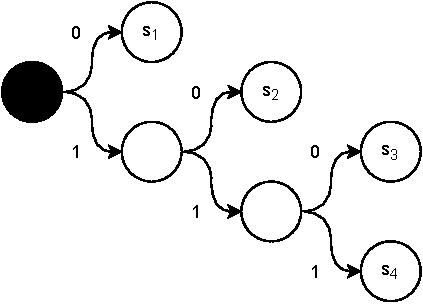
\includegraphics[scale = 0.8]{img/ct.pdf}
\end{figure}
Avendo che ogni cammino dalla radice ad una voglia è una codeword con la
foglia etichettata con il simbolo relativo alla codeword. Si ha quindi un
sottoalbero per ogni simbolo di $\Gamma$ (quindi dalla radice escono
$|\Gamma|$ archi) e da ogni nodo interno esce un numero
di archi minore o uguale al numero di simboli. Il ricevente sfrutta l'albero di
decodifica.\\ 
Posso anche usare l'albero per costruire il codice istantaneo.\\
Inoltre dato che un codice istantaneo è associato ad un albero di codifica non
succede mai che una codeword sia prefissa di un'altra (e lo si vede non prendo
avere due foglie associate a due codeword una prefissa dell'altra).
\begin{esempio}
  Vediamo l'albero di decodifica di un codice non istantaneo.\\
  Si hanno:
  \begin{itemize}
    \item $s_1\to 0$
    \item $s_2\to 01$
    \item $s_3\to 011$
    \item $s_4\to 111$
  \end{itemize}
  Si ha:
  \begin{figure}[H]
    \centering
    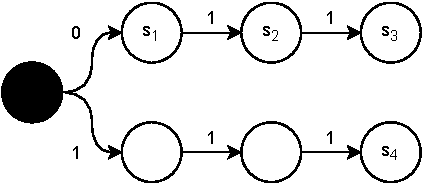
\includegraphics[scale = 0.8]{img/ct2.pdf}
  \end{figure}
  Avendo foglie che sono prefisse di altre.
\end{esempio}
Se devo costruire un codice istantaneo posso quindi usare un \textbf{comma code}
o costruire un albero di decodifica che sia il più possibile simile ad un albero
completo.
\begin{esempio}
  Si supponga di avere le seguenti codeword binarie per 5 simboli $s_i$:
  \begin{itemize}
    \item $s_1\to 0$
    \item $s_2\to 10$
    \item $s_3\to 110$
    \item $s_4\to 1110$
    \item $s_4\to 11110$
  \end{itemize}
  Si ha quindi:
   \begin{figure}[H]
    \centering
    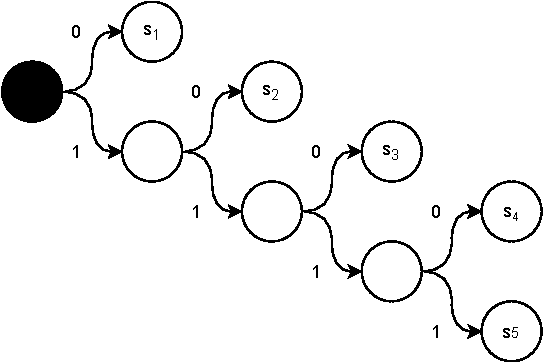
\includegraphics[scale = 0.8]{img/ct3.pdf}
  \end{figure}
  (e si nota come si possa generalizzare l'albero per un comma code).
\end{esempio}
\begin{esempio}
  Avendo l'albero:
    \begin{figure}[H]
    \centering
    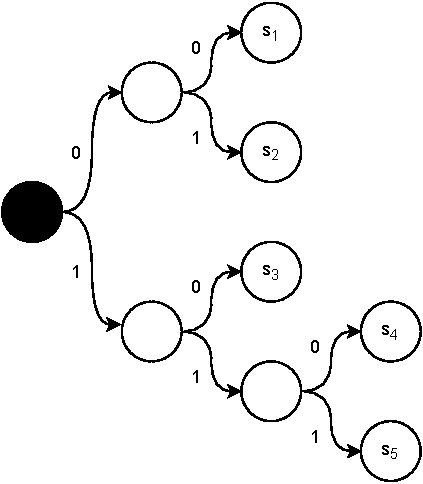
\includegraphics[scale = 0.7]{img/ct4.pdf}
  \end{figure}
  Riconosco il codice:
  \begin{itemize}
    \item $s_1\to 00$
    \item $s_2\to 01$
    \item $s_3\to 10$
    \item $s_4\to 110$
    \item $s_5\to 111$
  \end{itemize}
  
\end{esempio}
\begin{esempio}
  Avendo il codice 1:
   \begin{itemize}
    \item $s_1\to 0$
    \item $s_2\to 10$
    \item $s_3\to 110$
    \item $s_4\to 1110$
    \item $s_5\to 11110$
  \end{itemize}
  e il codice 2:
   \begin{itemize}
    \item $s_1\to 00$
    \item $s_2\to 01$
    \item $s_3\to 10$
    \item $s_4\to 110$
    \item $s_5\to 111$
  \end{itemize}
  assegno ad entrambi le probabilità:
   \begin{itemize}
    \item $p_1\to 0.9$
    \item $p_2\to 0.025$
    \item $p_3\to 0.025$
    \item $p_4\to 0.025$
    \item $p_5\to 0.025$
  \end{itemize}
  Ho che, per il primo codice:
  \[L_1=0.9\cdot 1+0.025\cdot 2+0.025\cdot 3+0.025\cdot 4+0.025\cdot 4=1.225\]
  Avendo che mediamente per rappresentare un simbolo della sorgente mi servono
  $1.225$ bit.\\
  Passo al secondo codice:
  \[L_2=0.9\cdot 2+0.025\cdot 2+0.025\cdot 2+0.025\cdot 3+0.025\cdot 3=2.05\]
  Avendo che mediamente per rappresentare un simbolo della sorgente mi servono
  $2.05$ bit.\\
  Ne segue, avendo $L_1<L_2$, per questa sorgente con queste probabilità è
  meglio il primo codice, il comma code.\\
  Se avessi avuto probabilità uniforme ($p_i=0.2$) avrei avuto:
  \[L_1=2.8\]
  \[L_2=2.4\]
  Essendo meglio il secondo codice.
\end{esempio}
\begin{definizione}
  Si definisce \textbf{codice r-ario} un codice con $r$ simboli con cui si
  ottengono le codeword.\\
  Un codice che parte da $\Gamma=\{0,1\}$ è un codice binario.
\end{definizione}
Ad un certo punto Kraft scopre un teorema che contiene una disuguaglianza che
fornisce una condizione necessaria e sufficiente affinché esista un codice
istantaneo con certe lunghezze $l_1,l_2,\ldots,l_n$ date.
\begin{teorema}[disuguaglianza di Kraft]
  Si ha che \textbf{esiste} un \textbf{codice istantaneo r-ario} per una
  sorgente $S$ di $q$ simboli, con codeword di lunghezza $l_1,l_2,\ldots,l_q$,
  sse: 
  \[\sum_{i=1}^q\frac{1}{r^{l_i}}\leq 1\]
  In onore di Kraft si ha che:
  \[K=\sum_{i=1}^q\frac{1}{r^{l_i}} \mbox{ e quindi } K\leq 1\]
  \textbf{Non si sta vedendo come sono fatte le codeword ma solo se può esistere
    un certo codice istantaneo. Sapendo che esiste poi bisogna costruire le
    codeword ma il teorema non dice nulla in merito.}\\
  La condizione necessaria e sufficiente è quindi una caratterizzazione
  dell'esistenza del codice istantaneo.
\end{teorema}
\begin{proof}
  Dobbiamo dimostrare i due versi del sse:
  \begin{enumerate}
    \item per ogni codice istantaneo r-ario di $q$ simboli con lunghezze
    $l_1,l_2,\ldots,l_q$ si ha che $K\leq 1$
    \item se $K\leq 1$ allora esiste un codice istantaneo con lunghezze
    $l_1,l_2,\ldots,l_q$ 
  \end{enumerate}
  Dimostriamo la \textbf{prima parte}.\\
  Prendo il codice e lo rappresento sull'albero di decodifica (dove ogni nodo ha
  al più $r$ archi uscenti). Ricorsivamente un albero o è vuoto o è un nodo che
  punta ad altri nodi.\\
  Parto con $r=2$, avendo codeword binarie su $\{0,1\}$ e di conseguenza alberi
  binari di decodifica. Procedo quindi con una dimostrazione per induzione sulla
  profondità dell'albero:
  \begin{itemize}
    \item \textbf{base}: profondità pari a 1. Si hanno due casi:
    \begin{enumerate}
      \item la radice o punta ad una foglia. In questo caso:
      \[K=\frac{1}{2^1}=\frac{1}{2}\leq 1\]
      \begin{figure}[H]
        \centering
        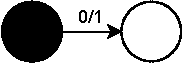
\includegraphics[scale = 0.7]{img/ct6.pdf}
      \end{figure}
      \item punta a due foglie (una per ogni simbolo). In questo caso:
      \[K=\frac{1}{2^1}+\frac{1}{2^1}=1\leq 1\]
      \begin{figure}[H]
        \centering
        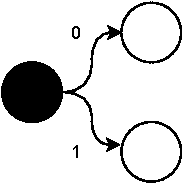
\includegraphics[scale = 0.7]{img/ct5.pdf}
      \end{figure}
    \end{enumerate}
    
    \item \textbf{passo induttivi}: assunto che il teorema è vero per ogni
    albero di profondità $n-1$ dimostriamo che il teorema vale anche per gli
    alberi di profondità $n$. In realtà così non ci va bene in quanto i
    sottoalberi dovrebbero avere entrambi profondità $n-1$ (cosa non vera come
    visto negli esempi precedenti, ad esempio ``l'\textit{albero a pettine}''
    del comma code). Cambiamo quindi dicendo che  assunto che il teorema è vero
    per ogni albero di profondità $<n$ dimostriamo che il teorema vale anche per
    gli alberi di profondità $n$.\\
    Considero i due sottoalberi come alberi a se stanti:
    \begin{figure}[H]
      \centering
      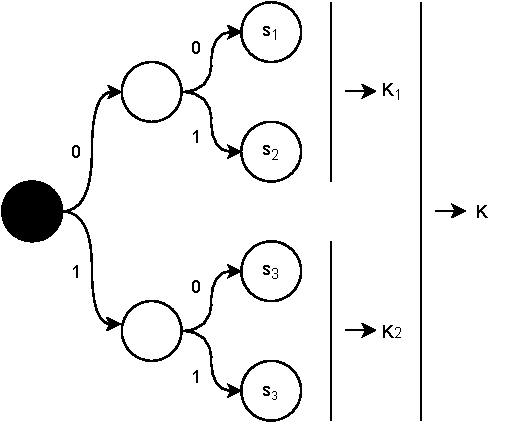
\includegraphics[scale = 0.7]{img/ct7.pdf}
    \end{figure}
    Dico che $K_1\leq 1$ per il primo sottoalbero e $K_2\leq 1$ per il secondo
    sottoalbero. \\
    Calcolo ora $K$ di tutto l'albero ma devo capire come si rapporta a $K_1$ e
    $K_2$. Si ha che se attacco il primo sottoalbero alla nuova radice per
    costruire l'albero globale ho che attacco ad ogni codeword un simbolo, che
    quindi si allungano di 1:
    \[\sum_{i=1}^q\frac{1}{r^{l_i+1}}\leq 1\]
    ma altro non è che:
    \[\sum_{i=1}^q\frac{1}{r}\cdot\frac{1}{r^{l_i}}\leq 1\]
    ma allora:
    \[\frac{1}{r}\cdot\sum_{i=1}^q\frac{1}{r^{l_i}}\leq 1=\frac{1}{r}\cdot K_1\]
    Faccio lo stesso per $K_2$ e quindi, avendo $r=2$:
    \[K=\frac{1}{2}\cdot K_1+\frac{1}{2}\cdot K_2\]
    ma sto sommando due quantità $\leq \frac{1}{2}$ (avendo $K_1\leq 1$ e
    $K_2\leq 1$) e quindi: 
    \[K\leq 1\]
  \end{itemize}
  Qualora si avesse $r>2$ si ha:
  \begin{itemize}
    \item \textbf{base}, si hanno alberi r-ari, con
    $\Gamma=\{0,1,2,\ldots,r-1\}$, di probabilità 1. Tutti questi alberi hanno
    $s$ foglie e $s-r$ non foglie. Quindi, essendo tutti gli $l_i$ uguali a 1
    essendo a profondità uno:
    \[K=\sum \frac{1}{r^{l_1}}=\sum \frac{1}{r}=\frac{s}{r}\leq 1\]
    $\frac{s}{r}\leq 1$ in quanto $s<r$
    \item \textbf{passo induttivo} si ha un albero r-ario a profondità $n$ con
    un certo numero di sottoalberi $s$ e un certo numero di sottoalberi vuoti,
    di cardinalità $s-r$, a profondità $n-1$. Per tutti i $K_1,K_2,\ldots K_s$
    ho che $K_i\leq 1$ e quindi ottengo $K$ aggiungendo un simbolo alle codeword 
    dei sottoalberi non vuoto (quelli vuoti contribuiscono con 0 alla
    sommatoria): 
    \[K=\frac{1}{r}K_1+\frac{1}{r}K_2+\cdots+\frac{1}{r}K_s\]
    Ma per lo stesso ragionamento del caso binario, essendo ogni $K_1<leq 1$ e
    quindi ogni componente della sommatoria è $\leq \frac{1}{r}$:
    \[K=\frac{1}{r}K_1+\frac{1}{r}K_2+\cdots+\frac{1}{r}K_s\leq \frac{s}{r}\leq
      1\] 
  \end{itemize}
  Vediamo la \textbf{seconda parte} della dimostrazione.\\
  Se $K\leq 1$ dobbiamo dimostrare che esiste un codice istantaneo con lunghezze
  $L_1,\ldots, l_q$.\\
  Sappiamo che:
  \[K=\sum_{i=1}^q\frac{1}{r^{l_i}}\leq 1\]
  Vediamo un esempio per capire come vedere diversamente la diseguaglianza:
  \begin{esempio}
    se avessi $r=2$, con quindi codeword binarie, e lunghezze 2,2,3,3,4 (con
    quindi $q=5$). Si ha che: 
    \[K=\frac{1}{2^2}+\frac{1}{2^2}+\frac{1}{2^3}+\frac{1}{2^3}+\frac{1}{2^4}\]
    Ma quindi:
    \[K=\frac{2}{2^2}+\frac{2}{2^3}+\frac{1}{2^4}\]
    Avendo ora 2,2,1 come numeratori.
  \end{esempio}

  Indico con $t_j$ il numero di codeword di lunghezza $j$. Si hanno quindi, per
  l'esempio precedente:
  \begin{itemize}
    \item $t_1=0$
    \item $t_2=2$
    \item $t_3=2$
    \item $t_4=1$
  \end{itemize}
  Riscrivo quindi $K$:
  \[K=\sum_{i=1}^q\frac{1}{r^{l_i}}=\sum_{j=1}^l\frac{t_j}{r^{j}}\]
  con $l=\max\{l_1,\ldots,l_q\}$ (per l'esempio sopra $l=4$).\\
  Si ha quindi che:
  \[\sum_{j=1}^l\frac{t_j}{r^{j}}\leq 1\]
  Ma posso dire che, per arrivare ad isolare i $t_j$ senza alterare la
  diseguaglianza: 
  \[r^l\cdot \sum_{j=1}^l\frac{t_j}{r^{j}}\leq 1\cdot r^l\]
  ma quindi ho che:
  \[r^l\cdot \sum_{j=1}^lt_j\cdot r^{l-j}\leq 1\cdot r^l\]
  Si ha che:
  \[ \sum_{j=1}^lt_j\cdot r^{l-j}= t_1\cdot r^{l-1}+\cdots+t_{l-1}\cdot
    r+t_l\leq r^l\]
  Ma quindi:
  \[t_l\leq r^l- t_1\cdot r^{l-1}-\cdots-t_{l-1}\cdot r\]
  ma so anche che:
  \[0\leq t_l\]
  e quindi:
  \[0\leq t_l\leq r^l- t_1\cdot r^{l-1}-\cdots-t_{l-1}\cdot r\]
  e quindi:
  \[0\leq r^l- t_1\cdot r^{l-1}-\cdots-t_{l-1}\cdot r\]
  porto quindi $t_{l-1}$ a sinistra e divido per $r$, ottenendo:
  \[t_{l-1}\leq r^{l-1}-t_1\cdot r^{l-1}-\cdots t_{l-2}\cdot r\]
  lo faccio per tutti i $t_j$ partendo da $t_{l-2}$ e arrivando a:
  \[t_2\leq r^2-t_1\cdot r\]
  sapendo per di più che:
  \[0\leq t_2\leq r^2-t_1\cdot r\]
  e poi a:
  \[0\leq t_1\leq r\]
  Risalgo quindi partendo dalle codeword più corte. Cerco $t_1$ codeword di
  lunghezza 1, avendo a disposizione l'alfabeto $\Gamma$ r-ario. Per farlo
  prendo i primi $t_1$ simboli e dico che sono le stringhe di lunghezza 1. Posso
  farlo perché $t_1\leq r$ e mi avanzano $r-t_1$ simboli dell'alfabeto.\\
  Passo alle codeword di lunghezza 2, me ne servono $t_2$. Queste codeword sono
  due simboli concatenati in modo che il primo simbolo non si stato utilizzato
  per $t_1$ (altrimenti creerei prefissi), quindi prendo un simbolo dai $r-t_1$
  simboli dell'alfabeto. Il secondo simbolo posso mettere un qualsiasi simbolo
  di $\Gamma$, avendo $r$ possibili scelte. In totale ho quindi un numero di
  combinazioni pari a:
  \[(r-t_1)\cdot r=r^2-t_1\cdot r\]
  e ho abbastanza combinazioni avendo che $t_2\leq r^2-t_1\cdot r$ per i conti
  precedenti. Le codeword le scelgo come voglio, ci sono tantissimi modi
  possibili.\\  
  Mi avanzano quindi $r^2-t_1\cdot r-t_2$.\\
  Creo le codeword di lunghezza 3 dove i primi due simboli non devono essere una
  combinazione usata per quelle di lunghezza 2, facendo poi gli stessi discorsi
  fatti sopra. \\
  Avanzo così per tutte le lunghezze di codeword avendo che posso costruire
  almeno un codice istantaneo, dimostrando la validità del teorema.
\end{proof}
\begin{esempio}
  Riprendiamo l'esempio di sopra.\\
  Si ha che: 
  \[K=\frac{1}{2^2}+\frac{1}{2^2}+\frac{1}{2^3}+\frac{1}{2^3}+\frac{1}{2^4}\]
  Ma quindi:
  \[K=\frac{2}{2^2}+\frac{2}{2^3}+\frac{1}{2^4}=\frac{3}{4}+\frac{1}{16}\leq 1\]
  \newpage
  Se volessi le codeword costruisco l'albero di decodifica:
  \begin{figure}[H]
    \centering
    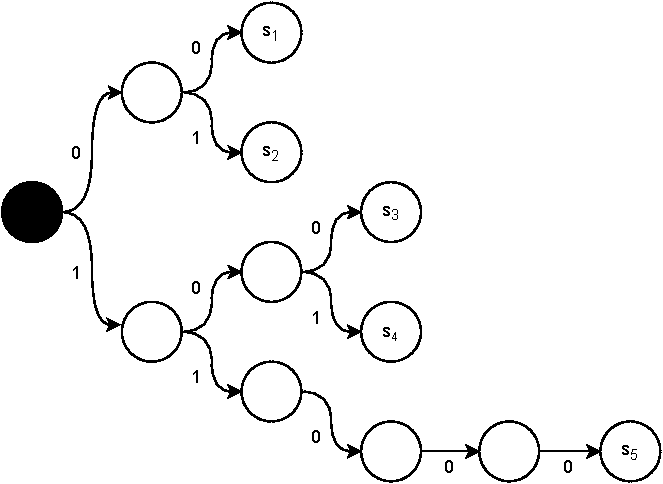
\includegraphics[scale = 0.7]{img/ct8.pdf}
  \end{figure}
  Avendo:
   \begin{itemize}
    \item $s_1\to 00$
    \item $s_2\to 01$
    \item $s_3\to 100$
    \item $s_4\to 101$
    \item $s_5\to 1100$
  \end{itemize}
  Ma vedo che ho nodi interni inutili (tipo i due nodi che portano a $s_5$).
  Butto via quindi i nodi con un solo ramo in uscita:
  \begin{figure}[H]
    \centering
    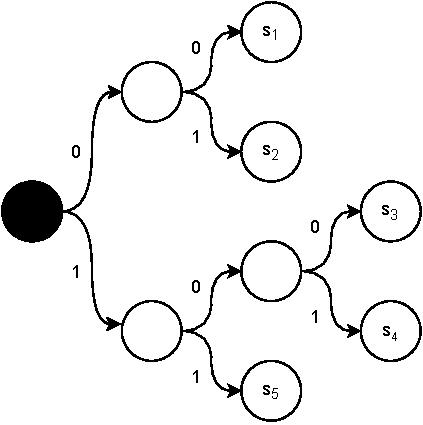
\includegraphics[scale = 0.7]{img/ct9.pdf}
  \end{figure}
  ottenendo:
  \begin{itemize}
    \item $s_1\to 00$
    \item $s_2\to 01$
    \item $s_3\to 100$
    \item $s_4\to 101$
    \item $s_5\to 11$
  \end{itemize}
  e quindi:
  \[K=\frac{3}{2^2}+\frac{2}{2^3}=\frac{3}{4}+\frac{1}{4}=1\leq 1\]
\end{esempio}
Quindi un nodo interno che solo un figlio mi fa allungare le lunghezze delle
codeword facendo sommare valori più piccoli. Se ho solo nodi interni con due
figli si può dimostrare per induzione che $K=1$ (nel caso base ho $K=1$ e in
quello induttivo vedo che ho $K_i=1$ per ogni sottoalbero, avendo poi che
$K=\frac{1}{2}K_1+\frac{1}{2}K_2=\frac{1}{2}\cdot 1+\frac{1}{2}\cdot 1= 1$).\\
Per tutti i codici istantanei vale che $K\leq 1$.
\subsection{Codici a Blocchi Accorciati}
Si vuole costruire un codice binario per un certo $q$.
\begin{esempio}
  Ipotizzo $r=2$ e
  $q=5$. Potrei avere tutte le 8 codeword di 3 bit ma ne scelgo solo $5$. Tengo
  $000,010,100,110,111$, avendo rimosso $001,011,101$. Queste 5 formano un
  codice a blocchi, istantaneo. Potrebbe non essere efficiente, non avendo
  $K=1$. Se costruissi l'albero avrei:
  \begin{figure}[H]
    \centering
    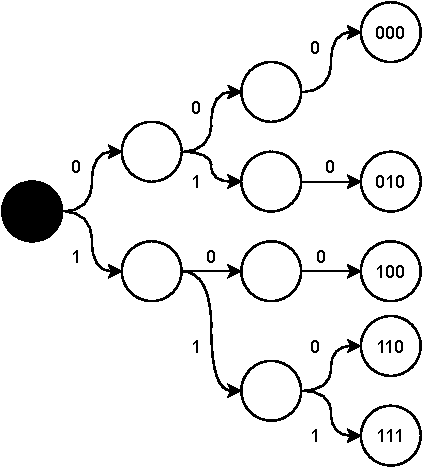
\includegraphics[scale = 0.7]{img/b.pdf}
  \end{figure}
  Che ha $K\neq 1$.
  \newpage
  Potrei rimuovere archi inutili, ottenendo:
  \begin{figure}[H]
    \centering
    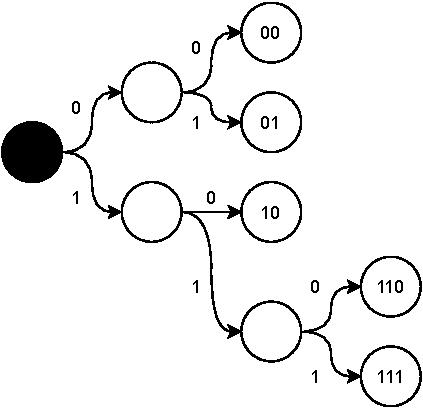
\includegraphics[scale = 0.7]{img/b2.pdf}
  \end{figure}
  Ottenendo:
  \begin{itemize}
    \item 00
    \item 01
    \item 10
    \item 110
    \item 111
  \end{itemize}
  Che non è più a blocchi ma è istantaneo con $K=1$ (ogni nodo interno ha
  infatti esattamente due figli).
\end{esempio}
Si sta parlando appunto di \textbf{codici a blocchi accorciati}.\\
\textbf{Su file esercizi esempio con codice non binario}.
\subsection{Disuguaglianza di McMillan}
\begin{teorema}[Disuguaglianza di McMillan]
  Data una sorgente $S=\{s_1,\ldots,s_q\}$ si ha che una condizione necessaria e
  sufficiente affinché esista un codice r-ario univocamente decodificabile con
  codeword di lunghezze $l_1,l\dots,l_q$ è che valga:
  \[K=\sum_{i=1}^q\frac{1}{r^{l_1}}\leq 1\]
  \textup{Quindi è uguale alla disuguaglianza di Kraft semplicemente sostituendo
  ``codici istantanei'' con ``codice univocamente decodificabile''.}
\end{teorema}
\begin{proof}
  Anche in questo caso si hanno i due versi della dimostrazione.\\
  La \textbf{prima parte} è dimostrare che dato un codice r-ario per $S$
  univocamente decodificabile allora $K\leq 1$ e per tale codice le lunghezze
  sono $l_1,l\dots,l_q$. Il ``dato'' è in realtà un ``per ogni''.\\
  Non posso più ragionare sulla profondità dell'albero non avendo più
  corrispondenza biunivoca con alberi dove le codeword sono le foglie. In questo
  caso avrei nodi interni che sono codeword, non posso quindi usare la stessa
  tecnica di dimostrazione.\\
  Per dimostrarlo prendo $K$ e un numero $n\in\mathbb{N}$, tale che
  $n>1$. Calcolo $K^n$, avendo:
  \[K^n=\left(\sum_{i=1}^q\frac{1}{r^{l_1}}\right)^n\]
  Ottenendo qualcosa di davvero difficile da studiare. Ma posso scrivere:
  \[K^n=\sum_{t=n}^{n\cdot l}\frac{n_t}{r^{t}}\]
  indicando con $n_t$ il numero di termini con $t$ (??? risentire) e con
  $l=\max\{l_1,\ldots,l_q\}$. Si ha che $n_t$ è anche il numero di codeword di
  lunghezza $t$. Ma dato che il codice è univocamente decodificabile si ha che:
  \[n_t\leq r^t\]
  ma allora:
  \[\frac{n_t}{r^{t}}\leq 1\]
  Ma allora si può dire, maggiorando, che:
  \[K^n=\sum_{t=n}^{n\cdot l}\frac{n_t}{r^{t}}\leq \sum_{t=n}^{n\cdot
      l}1=n\cdot l-n+1=n\cdot l-(n-1)\]
  Ma $(n-1)>0$ e quindi:
  \[=n\cdot l-(n-1) < n\cdot l\]
  E quindi:
  \[K^n<n\cdot l\]
  \newpage
  Questo si risolve graficamente (\textbf{grafico molto approssimato}):
  \begin{figure}[H]
    \centering
    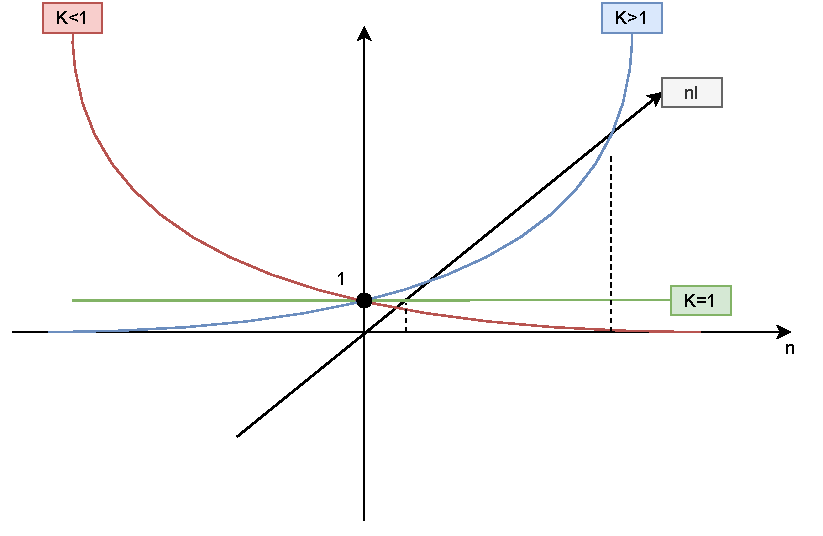
\includegraphics[scale = 0.8]{img/grap.pdf}
  \end{figure}
  Se $K>1$ ad un certo punto la curva supera $n\cdot l$. Per $K<1$ sicuramente
  ho punti per cui è $<n\cdot l$ e quindi si arriva a dire che:
  \[K^n<n\cdot l\implies K\leq 1\]
  dimostrando la tesi.\\
  
  La \textbf{seconda parte} è che se $K\leq 1$ allora esiste un codice r-ario
  per $S$ univocamente decodificabile con lunghezze $l_1,l\dots,l_q$. Per Kraft,
  avendo $K\leq 1$ esiste un codice istantaneo per $S$, r-ario, con tali
  lunghezze. Ma \textbf{un codice istantaneo è univocamente decodificabile},
  avendo quindi dimostrato la tesi.
\end{proof}
Ma avendo che i codici univocamente decodificabili sono meno utili di quelli
istantanei vengono trascurati, considerando che dovrei fare la ``stessa
fatica''.\\
Abbiamo visto comunque che non si hanno indicazioni in merito a come fare le
codeword e abbiamo anche trascurato finora l'uso delle probabilità.
\subsection{Codici di Huffman}
I codici di Huffman sono ottimali, ovvero raggiungono il minimo valore possibile
della lunghezza media $L$:
\[L=\sum_{i=1}^q p_i\cdot l_i\]
\begin{teorema}
  In input abbiamo quindi il codice $S$, con $s_i,\ldots s_q$, con probabilità
  $p_1,\ldots, p_q$. Il codice di Huffman ci restituisce in output sia le
  lunghezze $l_i$ che le codeword $\gamma_i$.\\
  Bisogna prima fare qualche ragionamento.\\
  Si supponga di avere i simboli in ordine di probabilità, avendo:
  \[p_1\leq p_2\leq \cdots\leq p_q\]
  ma quindi si ha che:
  \[l_1\leq l_2\leq \cdots \leq l_q\]
  perché altrimenti non avrei il codice ottimale.
\end{teorema}
\begin{proof}
  Si supponga infatti di avere
  $p_m>p_n$ e $l_m>l_n$. Studio quindi il contributo dei due simboli:
  \[p_m\cdot l_m+p_n\cdot l_n\]
  Scambio in modo che $p_m$ riceva la codeword $l_n$:
  \[p_m\cdot l_n+p_n\cdot l_m\]
  Faccio la differenza:
  \[(p_m\cdot l_n+p_n\cdot l_m)-(p_m\cdot l_m+p_n\cdot l_m)\]
  \[=p_m\cdot (l_n-l_m)-p_n\cdot (l_n-l_m)\]
  \[=(p_m-p_n)\cdot(l_n-l_m)\]
  Ma abbiamo che $p_m>p_n$ e quindi $(p_m-p_n)>0$ e per lo stesso ragionamento,
  avendo $l_m>l_n$, $(l_n-l_m)<0$. Si ha quindi che:
  \[(p_m\cdot l_n+p_n\cdot l_m)-(p_m\cdot l_m+p_n\cdot l_m)<0\]
  e quindi:
  \[p_m\cdot l_n+p_n\cdot l_m<[p_m\cdot l_m+p_n\cdot l_n\]
  perdendo quindi l'ottimalità del codice. 
\end{proof}
Deve quindi valere:
\[p_1\leq p_2\leq \cdots\leq p_q\]
e
\[l_1\leq l_2\leq \cdots \leq l_q\]
Si ha quindi un algoritmo greedy per ottimizzare la lunghezza media. Non
sappiamo se si ha un matroide ma si vedrà che tale algoritmo porta
all'ottimo. Vediamo in primis un esempio.
\begin{esempio}
  Vediamo un esempio di questo algoritmo:\\
  Presa una sorgente con $5$ simboli con le annesse probabilità (sono già
  ordinati): 
  \begin{itemize}
    \item $s_1$ con $p_1=0.4$
    \item $s_2$ con $p_2=0.2$
    \item $s_3$ con $p_3=0.2$
    \item $s_4$ con $p_4=0.1$
    \item $s_5$ con $p_5=0.1$
  \end{itemize}
  Si assuma $r=2$.\\
  Prendo i due simboli meno probabili e li unisco creando un nuovo simbolo
  ``fittizio'' con probabilità pari alla somma dei due (nel nostro caso quindi
  $0.1+0.1=0.2$). Si ha quindi, mantenendo sempre l'ordine (metto il simbolo
  combinato in coda a parità di probabilità):
  \begin{itemize}
    \item $s_1$ con $p_1=0.4$
    \item $s_2$ con $p_2=0.2$
    \item $s_3$ con $p_3=0.2$
    \item $s_{4,5}$ con $p_{4,5}=0.2$
  \end{itemize}
  Avendo ora una nuova sorgente di 4 simboli (quindi ipoteticamente più semplice
  da codificare di quella da $5$).\\
  Itero facendo la stessa cosa:
  \begin{itemize}
    \item $s_1$ con $p_1=0.4$
    \item $s_{3,4,5}$ con $p_{3,4,5}=0.4$
    \item $s_2$ con $p_2=0.2$
  \end{itemize}
  Avendo ora 3 simboli. Proseguo:
  \begin{itemize}
    \item $s_{2,3,4,5}$ con $p_{2,3,4,5}=0.6$
    \item $s_1$ con $p_1=0.4$
  \end{itemize}
  Che è facile da codificare, associando 0 e 1 (l'ordine è opzionale):
  \begin{itemize}
    \item $s_{2,3,4,5}$ con $p_{2,3,4,5}=0.6$: 0
    \item $s_1$ con $p_1=0.4$: 1
  \end{itemize}
  Costruisco quindi la sorgente a 3 (usando 0 come prefisso di tutti i nuovi):
  \begin{itemize}
    \item $s_1$ con $p_1=0.4$: 1
    \item $s_{3,4,5}$ con $p_{3,4,5}=0.4$: 00
    \item $s_2$ con $p_2=0.2$: 01 (infatti 10 non andrebbe bene avendo 1 come prefisso)
  \end{itemize}
  proseguo (usando 00 come prefisso di tutti i nuovi):
    \begin{itemize}
    \item $s_1$ con $p_1=0.4$: 1
    \item $s_2$ con $p_2=0.2$: 01
    \item $s_3$ con $p_3=0.2$: 000
    \item $s_{4,5}$ con $p_{4,5}=0.2$: 001
  \end{itemize}
  termino con lo stesso ragionamento (avendo ora 001 come prefisso):
  \begin{itemize}
    \item $s_1$ con $p_1=0.4$: 1
    \item $s_2$ con $p_2=0.2$: 01
    \item $s_3$ con $p_3=0.2$: 000
    \item $s_4$ con $p_4=0.1$: 0010
    \item $s_5$ con $p_5=0.1$: 0011
  \end{itemize}
  Che ha:
  \[L=0.4\cdot 1+0.2\cdot 2+0.2\cdot 3+0.1\cdot 4+0.1\cdot 4 =
    2.2\frac{bit}{simbolo}\]
  Se invece metto i nuovi simboli più in alto possibile avrei:
  \begin{itemize}
    \item $s_1$ con $p_1=0.4$
    \item $s_{4,5}$ con $p_{4,5}=0.2$
    \item $s_2$ con $p_2=0.2$
    \item $s_3$ con $p_3=0.2$
  \end{itemize}
  e quindi:

  \begin{itemize}
    \item $s_{2,3}$ con $p_{2,3}=0.4$
    \item $s_1$ con $p_1=0.4$
    \item $s_{4,5}$ con $p_{4,5}=0.2$
  \end{itemize}
  e quindi:

  \begin{itemize}
    \item $s_{1,4,5}$ con $p_{1,4,5}=0.6$
    \item $s_{2,3}$ con $p_{2,3}=0.4$
  \end{itemize}
  Procedendo come nel caso precedente sopra si avrebbe (\textbf{verificare i
    passaggi}): 
   \begin{itemize}
    \item $s_{1,4,5}$ con $p_{1,4,5}=0.6$: 0
    \item $s_{2,3}$ con $p_{2,3}=0.4$: 1
  \end{itemize}
  e quindi:
  \begin{itemize}
    \item $s_{2,3}$ con $p_{2,3}=0.4$: 1
    \item $s_1$ con $p_1=0.4$: 00
    \item $s_{4,5}$ con $p_{4,5}=0.2$: 01
  \end{itemize}
  e quindi:
  \begin{itemize}
    \item $s_1$ con $p_1=0.4$: 1
    \item $s_{4,5}$ con $p_{4,5}=0.2$: 01
    \item $s_2$ con $p_2=0.2$: 000
    \item $s_3$ con $p_3=0.2$: 001
  \end{itemize}
  e infine:
  \begin{itemize}
    \item $s_1$ con $p_1=0.4$: 00
    \item $s_2$ con $p_2=0.2$: 10
    \item $s_3$ con $p_3=0.2$: 11
    \item $s_4$ con $p_4=0.1$: 010
    \item $s_5$ con $p_5=0.1$: 011
  \end{itemize}
  Che ha:
  \[L=0.4\cdot 2+0.2\cdot 2+0.2\cdot 2+0.1\cdot 3+0.1\cdot 3 =
    2.2\frac{bit}{simbolo}\]
  che è uguale a prima.
\end{esempio}
\textit{Questo algoritmo greedy funziona, producendo l'ottimo, quando
  sottostante al problema si ha un matroide.}
\begin{teorema}
  Si può dimostrare che non cambia nulla, in termini di lunghezza media,
  mettendo il nuovo simbolo il più in alto/basso possibile, a parità di
  probabilità.\\
  Si può anche
  dimostrare che se metto il simbolo combinato in basso aumenta la varianza tra
  le codeword (avendo codeword di lunghezza più ``distante'') mentre mettendoli
  più in alto possibile si diminuisce la varianza. SI ricorda che la varianza è:
  \[V=\sum_{i=1}^q p_i\cdot (l_i-L)^2\]
\end{teorema}
\textbf{Esempi sul file di esercizi}.\\
\textit{Solitamente comunque si preferisce abbassare la varianza tenendo quindi
  il nuovo simbolo più in alto possibile.}
\begin{teorema}
  Il codice di Huffman è ottimo, avendo la minor lunghezza media. In altri
  termini produce codici istantanei ottimali.
\end{teorema}
\begin{proof}
  Si procede per assurdo.\\
  Si ricorda che le lunghezza vengono conosciute solo a fine algoritmo di
  calcolo.\\ 
  Supponiamo, data una sorgente $S$ con $q$ simboli $s_1,\ldots,s_q$, con
  $p_1,\ldots, p_q$, che $l_1,\ldots, l_q$ siano le lunghezze di Huffman, avendo
  quindi in corrispondenza $L_H$, lunghezza di Huffman, come:
  \[L_H=\sum_{i=1}^q p_i\cdot l_i\]
  Se non fosse ottimo avremmo un altro codice con una migliore lunghezza media
  $L'$, tale che $L'< L_H$. Entrambi sono codici istantanei con associati i due
  alberi di decodifica. Prendo quindi i due simboli meno probabili (che sono
  anche i più lunghi) per il codice di Huffman: $s_q$ e $s_{q-1}$. Si potrebbe
  dimostrare che la lunghezza delle due codeword più lunghe è uguale. Questi due
  simboli sono presi, a parità di probabilità, in modo che condividano il nodo
  genitore nell'albero. Si ha che $l_q=l_{q-1}$, condividendo il genitore e non
  avendo nodi ``sprecati'' nell'albero di decodifica.\\
  Collasso questi due nodi e il genitore in un solo simbolo fittizio che tiene
  conto di entrambi i simboli. In pratica faccio uno dei ``passi in avanti''
  dell'algoritmo sopra specificato per il calcolo dei codici di Huffman. La
  lunghezza decresce di una certa quantità $x$. Si ha in partenza che
  $p_{q-1}\cdot l_{q-1}+p_q\cdot l_q=l_q\cdot (p_{q-1}+p_q)$. Il nuovo simbolo
  avrà:
  \[(l_q-1)\cdot (p_{q-1}+p_q)=l_q\cdot (p_{q-1}+p_q)- (p_{q-1}+p_q)\]
  ovvero la stessa quantità di prima meno $(p_{q-1}+p_q)$. Quindi dalla
  lunghezza media tiro via questa quantità, ovvero $x=(p_{q-1}+p_q)$.\\
  Se vogliamo minimizzare la lunghezza media il simbolo con $p_i$ più alta ha
  $l_i$ più bassa (come dimostrato precedentemente).\\
  Faccio lo stesso ragionamento nell'altro codice (che suppongo per assurdo
  migliore di quello di Huffman e quindi essendo ottimale vale lo stesso
  rapporto tra $p_i$ e $l_i$), prendendo $s_q'$ e
  $s_{q-1}'$ (che sono quelli con probabilità minore, lunghezza maggiore nel
  secondo codice e lunghezza uguale), fondendoli in un nuovo simbolo
  fittizio, facendo gli stessi ragionamento fatto per il codice di Huffman.
  Si ha in partenza che $p_{q-1}\cdot l_{q-1}+p_q\cdot l_q=l_q\cdot
  (p_{q-1}+p_q)$.  
  Il nuovo simbolo avrà:
  \[(l_q-1)\cdot (p_{q-1}+p_q)=l_q\cdot (p_{q-1}+p_q)- (p_{q-1}+p_q)\]
  La riduzione della lunghezza quindi è la stessa che nel caso di Huffman 
  $L_H-x$ e $L'-x$.\\ 
  Si stanno ``collassando'' gli stessi simboli e le lunghezze medie decrescono
  della stessa quantità.\\
  Ad un certo punto da entrambe le parti si arriva ad avere due
  simboli. Nell'albero si avranno quindi la radice e due simboli fittizi. Per il
  secondo codice si avrà comunque una sorgente con due figli e basta. \\
  Per Huffman so che ho due codeword di lunghezza 1 (un ramo con 0 e uno con 1)
  e quindi $L_h=1$ ma sotto questo valore non posso andare, non posso codificare
  due codeword che mi portino ad una lunghezza media $<1$ per il secondo codice
  che quindi ha lunghezza media pari a $1$. Si è dimostrato che l'assurdo è
  impossibile e quindi l'algoritmo di Huffman produce codici ottimali.
\end{proof}
\subsubsection{Codici di Huffman r-ari}
Vediamo ora i codici di Huffman per $r>2$.\\
\begin{esempio}
  Vogliamo un codice r-ario con $r=4$ e quindi $\Gamma=\{0,1,2,3\}$ con una
  sorgente di $q=8$ simboli. Si hanno le seguenti probabilità:
  \begin{itemize}
    \item $p_0=0.22$
    \item $p_1=0.20$
    \item $p_2=0.28$
    \item $p_3=0.15$
    \item $p_4=0.10$
    \item $p_5=0.08$
    \item $p_6=0.05$
    \item $p_7=0.02$
  \end{itemize}
  In questo caso non fondo gli ultimi due simboli ma gli ultimi 4. Al primo
  passo ottengo:
  \begin{itemize}
    \item $p_{4,5,6,7}=0.25$
    \item $p_0=0.20$
    \item $p_1=0.28$
    \item $p_2=0.15$
    \item $p_3=0.10$
  \end{itemize}
  e poi:
  \begin{itemize}
    \item $p_{0,1,2,3}=0.75$
    \item $p_{4,5,6,7}=0.25$
  \end{itemize}
  Associo 0 e 1:
    \begin{itemize}
    \item $p_{0,1,2,3}=0.75$: 0
    \item $p_{4,5,6,7}=0.25$: 1 
  \end{itemize}
  ricostruisco usando tutti e 4 i simboli:
    \begin{itemize}
    \item $p_{4,5,6,7}=0.25$: 1
    \item $p_0=0.20$: 00
    \item $p_1=0.28$: 01
    \item $p_2=0.15$: 02
    \item $p_3=0.10$: 03
  \end{itemize}
  e infine:
  \begin{itemize}
    \item $p_0=0.22$: 00
    \item $p_1=0.20$: 01
    \item $p_2=0.28$: 02
    \item $p_3=0.15$: 03
    \item $p_4=0.10$: 10
    \item $p_5=0.08$: 11
    \item $p_6=0.05$: 12
    \item $p_7=0.02$: 13
  \end{itemize}
  \textbf{Ma questo non è ottimale}, infatti potrei dire che $13$ è 2 e che $12$
  è $3$ che non sono prefissi, per esempio. Questo succede perché nell'ultimo
  step ho usato solo 0 e 1 e non tutti i simboli possibili della sorgente,
  perdendo diverse codeword. Voglio quindi arrivare all'ultimo step con
  esattamente 4 simboli. Per farlo aggiungo simboli fittizi alla sorgente in
  modo che raccogliendo a botte di $r$ si arrivi alla fine con $r$ simboli.\\
  Si ha ad esempio:
  \begin{itemize}
    \item $p_0=0.22$
    \item $p_1=0.20$
    \item $p_2=0.28$
    \item $p_3=0.15$
    \item $p_4=0.10$
    \item $p_5=0.08$
    \item $p_6=0.05$
    \item $p_7=0.02$
    \item $p_8=0$
    \item $p_9=0$
  \end{itemize}
  Al primo passo ottengo:
  \begin{itemize}
    \item $p_0=0.22$
    \item $p_1=0.20$
    \item $p_2=0.28$
    \item $p_3=0.15$
    \item $p_4=0.10$
    \item $p_5=0.08$
    \item $p_{6,7,8,9}=0.07$
  \end{itemize}
  e poi:
  \begin{itemize}
    \item $p_{3,4,5,6,7,8,9}=0.40$
    \item $p_0=0.22$
    \item $p_1=0.20$
    \item $p_2=0.28$
  \end{itemize}
  associo quindi i simboli:
   \begin{itemize}
    \item $p_{3,4,5,6,7,8,9}=0.40$: 0
    \item $p_0=0.22$: 1
    \item $p_1=0.20$: 2
    \item $p_2=0.28$: 3
  \end{itemize}
  avendo:
  \begin{itemize}
    \item $p_0=0.22$: 1
    \item $p_1=0.20$: 2
    \item $p_2=0.28$: 3
    \item $p_3=0.15$: 00
    \item $p_4=0.10$: 01
    \item $p_5=0.08$: 02
    \item $p_{6,7,8,9}=0.07$: 03
  \end{itemize}
  e quindi:
  \begin{itemize}
    \item $p_0=0.22$: 1
    \item $p_1=0.20$: 2 
    \item $p_2=0.28$: 3
    \item $p_3=0.15$: 00
    \item $p_4=0.10$: 01
    \item $p_5=0.08$: 02
    \item $p_6=0.05$: 030
    \item $p_7=0.02$: 031
    \item $p_8=0$: 032
    \item $p_9=0$: 033
  \end{itemize}
  Ma le ultime due non mi servono:
  \begin{itemize}
    \item $p_0=0.22$: 1
    \item $p_1=0.20$: 2 
    \item $p_2=0.28$: 3
    \item $p_3=0.15$: 00
    \item $p_4=0.10$: 01
    \item $p_5=0.08$: 02
    \item $p_6=0.05$: 030
    \item $p_7=0.02$: 031
  \end{itemize}
  \textbf{Che è ottimale}.\\
  Si può calcolare che:
  \[L=1.47\,\,\,simboli\,\,\, quaternari\]
\end{esempio}
Si dimostra che si ottengono con questo processo codici ottimali e si dimostra
in modo analogo al caso binario con $r=2$ (avendo che si ragiona non con due
figli ma con $r$ figli).\\
Capiamo meglio quanti simboli fittizi con probabilità nulla vanno aggiunti.
Avendo $q$ simboli mi serve un numero, che sia il minore possibile, $q'$ di
simboli tale che $q'\geq q$. Devo quindi aggiungere $q'-q$ simboli fittizi con
probabilità 0. In ogni passo tolgo $r$ simboli e ne aggiungo 1, quindi ne tolgo
$r-1$. Partendo da $q'$ diventano poi $q'-(r-1)$ e poi $q'-(r-1)-(r-1)$ e così
via. Alla fine voglio che ne restino $r$. Partendo dal fondo ho $r+(r-1)$ poi
$(r+2\cdot (r-1))$ etc$\ldots$ Si ha quindi che, per un certo $k$:
\[q'=k\cdot(r-1)+r\]
Ma posso togliere il numero $K$ di passi:
\[q'=(k+1)\cdot (r-1)+1\to q' \equiv 1\bmod (r-1)\]
Quindi devo trovare il più piccolo $q'\geq q$ tale che $q'$ è congruo a $1\bmod
(r-1)$. Al massimo dovrò mettere $r-1$ simboli fittizi.
\begin{shaded}
  Si ricorda che:
  \[a\equiv b\bmod n\iff \exists z\in\mathbb{Z}\mbox{ t.c. }a-b=z\cdot n\]
\end{shaded}
\begin{esempio}
  Nell'esempio sopra avevamo $q=8$ e $r=4$. Mi serve $q'\geq 8$ tale che $q'$ è
  congruo a $1\bmod 3$. I primi numeri congrui a $1\bmod 3$ sono:
  \[\{1,4,7,10\}\]
  e il più piccolo $\geq 8$ è 10 e quindi $q'=10$ e quindi $q'-q=2$. 
\end{esempio}
\textbf{Per $r=2$ facendo i conti si vede che arrivo sempre ad avere sempre e
  solo due simboli nell'ultimo passaggio}.\\
Si nota che posso codificare le cifre quaternarie tramite quelle binarie, $0\to
00$, $1\to 01$, $2\to 10$ e $3\to 11$, passando da uno a due simboli,
raddoppiando quindi anche le lunghezze delle codeword e il doppio della
lunghezza media, raggiungendo però un codice non ottimale (applicando
direttamente l'algoritmo di Huffman con $r=2$ si può dimostrare si ottiene un
codice migliore, avendo codeword di lunghezza due e tre e non due e quattro).\\
\begin{algorithm}
  \begin{algorithmic}
    \Function{Huffman}{$S=\{s_1,s_2,\ldots,s_n\},\,\,\, F$}
    \State $Q\gets \emptyset$
    \State \textit{inserire tutti gli} $s_i$ \textit{in} $Q$
    \For{$i\gets 1$ \textbf{to} $|S|$}
    \State \textit{alloca un nodo} $n$
    \State $left[n]\gets x\gets\mbox{extract\_min(Q)}$
    \State $right[n]\gets y\gets \mbox{extract\_min(Q)}$
    \State $F(n)\gets F(x)+F(z)$
    \State $Q.insert(n)$
    \EndFor
    \EndFunction
  \end{algorithmic}
  \caption{Pseudocodice dell'algoritmo di Huffman, con $S$ insieme dei simboli,
  $F$ che associa una frequenza ad ogni simbolo, $Q$ coda di priorità. Il codice
  non è stato trattato in aula ma mi sembrava interessante averlo.}
\end{algorithm}
Finora le sorgenti funzionavano che ad ogni colpo di clock uscisse un simbolo,
con probabilità associata, ignorando quanto successo prima. Si ha quindi che
queste sorgenti sono \textbf{memoryless}. 
\begin{definizione}
  Definiamo una \textbf{sorgente con memoria}.\\
  SU supponga di avere una memoria di ordine $j$. Si ha che il simbolo $s_i$
  esce con probabilità:
  \[p(s_i|s_{i1},s_{i2},\ldots,s_{ij})\]
  in pratica la probabilità di un simbolo è condizionata dai $j$ simboli usciti
  precedentemente. Questa è una sorgente con memoria.\\
  Il loro studio avviene tramite \textbf{processi di Markov} e
  \textbf{matrici}.\\
  Si cerca una distribuzione di probabilità, espressa tramite vettore, $\pi$
  tale che $\pi=M\pi$, con $M$ matrice. Si vuole quindi che ciascun simbolo esce
  con la probabilità indicata nel vettore $\pi$ in modo che sia un \textbf{punto
    fisso} (???). \\
  \textbf{\textit{Spiegazione superficiale in quanto al tematica non viene
      approfondita.}} 
\end{definizione}
L'algoritmo di Huffman si può adattare alle sorgenti con memoria.
\section{L'informazione}
Si ha sempre una sorgente $S$ senza memoria con i simboli $s_i$ a cui sono
associate le probabilità $p_i$. Cerchiamo di capire quanta informazione ci dà un
simbolo:
\[I(s_i)=?\]
L'informazione dipende soprattutto dal destinatario, da quanto è in grado di
comprendere tale informazione. Cambiare ricevente cambia tale valore.\\
Si arriverà a capire quanto si può comprimere un messaggio tramite la quantità
di informazione ma studiando solo dal punto di vista del messaggio ignorando il
ricevente.\\
Studiamo il rapporto tra $p_i$ e $I(s_i)$. Shannon dice che eventi più rari
forniscono una maggior quantità di informazione, essendo inversamente
proporzionale: 
\[I(s_i)=\frac{1}{p_i}\]
Si vuole anche che da due sottosistemi che producono due quantità di
informazioni $I(A)$ e $I(B)$ si possa ottenere l'informazione totale del
sistema $C$. Si vuole che valga l'additività:
\[I(C)=I(A)+I(B)\]
In realtà possiamo dire che che $I$ prende in input la probabilità stessa,
avendo:
\[I(p_i)=\frac{1}{p_i}\]
Se ho a che fare con due eventi indipendenti ho che:
\[I(p_i\cdot p_j)=\frac{1}{p_i\cdot p_j}\]
ma ho che $[I(p_i)=\frac{1}{p_i}$ e $I(p_j)=\frac{1}{p_j}$ e quindi vorrei:
\[I(p_i\cdot p_j)=\frac{1}{p_i\cdot
    p_j}=\frac{1}{p_i}+\frac{1}{p_j}=\frac{p_i+p_j}{p_i\cdot p_j}\neq
  \frac{1}{p_i\cdot p_j}\]
e quindi non va bene.\\
Ma l'additività la hanno potenze e logaritmi, quindi si dice che:
\[I(p_i)=\log_2\frac{1}{p_i}\]
Ma quindi:
\[I(p_i\cdot p_j)=\log_2\frac{1}{p_i\cdot
    p_j}=\log_2\left(\frac{1}{p_i}\cdot\frac{1}{p_j}\right)=
  \log_2\frac{1}{p_i}+\log_2\frac{1}{p_j}=I(p_i)+I(p_j)\]
Dal punto di vista assiomatico chiediamo che la quantità di informazione goda di
queste proprietà, avendo $I:[0,1]\to\mathbb{R}_0^+$:
\begin{itemize}
  \item $I(p)>0$
  \item $I(p_1\cdot p_2)=I(p_1)+I(p_2)$ se gli eventi sono indipendenti, valendo
  l'additività 
  \item $I(p)$ è una funzione continua, per non avere situazioni scomode
\end{itemize}
Già solo con queste proprietà se ne ricavano altre:
\begin{itemize}
  \item $I(P^n)=n\cdot I(p),\forall n\in \mathbb{N}$ e si potrebbe dimostrare
  per induzione. $I(P^1)=1\cdot I(P)$ e \[I(p^n)=I(p^{n-1}\cdot
    p)=I(P^{n-1})+I(p)=I(p)+(n-1)\cdot I(p)=n\cdot I(p)\]
  \item $y=p^n\to p=y^{\frac{1}{n}}$ e quindi:
  \[I(y)=I(p^n)=n\cdot I(p)=n\cdot I(y^{\frac{1}{n}})\]
  e quindi:
  \[I(y^{\frac{1}{n}})=\frac{1}{n}I(y)\]
  \item $I(y^\frac{m}{n})= I((y^{\frac{1}{n}})^m)=m\cdot
  I(y^{\frac{1}{m}})=\frac{m}{n}I(y)$ 
\end{itemize}
\begin{teorema}
  La funzione $I(p_i)$ è unica, ovvero è l'unica funzione che soddisfa le prime
  tre proprietà. 
\end{teorema}
\begin{proof}
  Ipotizzo che esista $g$ tale che $g(p^n)=n\cdot g(p)$. Si ha che $I(p)=c\cdot
  \log_2\frac{1}{p}$ per un certo $c$ costante. Si ha che, avendo $I(p^n)=c\cdot
  \log_2\frac{1}{p^n}$:
  \[g(p^n)-c\log_2\frac{1}{p^n}=n\cdot[g(p)-c\cdot \log_2 \frac{1}{p}]\]
  pongo, per un certo $p_0\neq 0,1$:
  \[c=\frac{g(p_0)}{\log_2\frac{1}{p_0}}\]
  in modo da ottenere, sostituendo, con $p=p_0$, ignorando traslazioni delle
  funzioni nel grafico
  \[g(p^n)-c\log_2\frac{1}{p^n}=n\cdot[g(p)-c\cdot \log_2 \frac{1}{p}]=0\]
  infatti:
  \[g(p_0)=I(p_0)\]
  Si ha che:
  \[\forall z\exists n\mbox{ t.c. }z=p_0^n\]
  Allora:
  \[g(z)-c\cdot \log_2\frac{1}{z}=0\implies g(z)=c\cdot\log_2\frac{1}{z}=I(z)\]
  dimostrando che:
  \[g(z)=I(z)\]
  \begin{figure}[H]
    \centering
    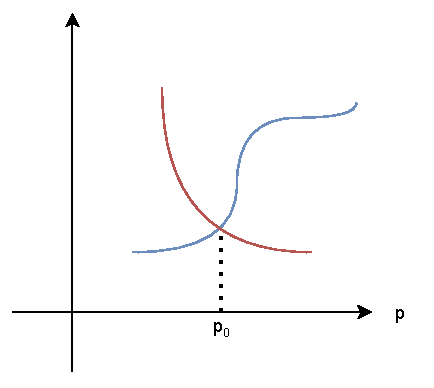
\includegraphics[scale = 0.6]{img/grap2.pdf}
    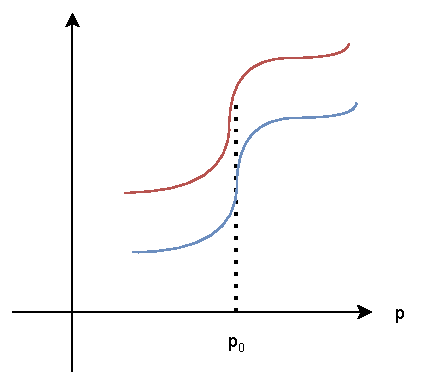
\includegraphics[scale = 0.6]{img/grap3.pdf}
    \caption{Grafici usati nella dimostrazione \textbf{da capire come}}
  \end{figure}
\end{proof}
L'unità di misura dell'informazione varia a seconda della base del logaritmo.\\
Si ha che $\log_2$ è l'unità di misura se ho a che fare con i bit (anche se
all'inizio 0 e 1 erano detti \textit{binit}) Misuro quindi in \textit{bit}. \\
Se ho $\log_e=\ln$ misuro in \textit{nat}.\\
Se ho $\log_{10}$ misuro in \textit{Hartley}.\\
La sorgente $s$ quindi emette il simbolo $s_i$ con $p_i$ e produce una quantità
di informazione pari a:
\[I(p_i)=\log_2\frac{1}{p_i}\]
e questo per ogni simbolo.\\
Si ha anche la quantità di informazione media della sorgente, facendo la media
pesata con le probabilità. Questa è detta \textbf{entropia} $H$:
\[H(S)=\sum_{i=1}^qp_i\cdot I(p_i)=\sum_{i=1}^qp_i\cdot \log_2\frac{1}{p_i}\]
spesso si usa $H_b$ con $b$ pari alla base del logaritmo, quindi:
\[H_2(S)=\sum_{i=1}^qp_i\cdot I(p_i)=\sum_{i=1}^qp_i\cdot \log_2\frac{1}{p_i}\]
Con $H_2$ funzione che ha in input tutte le probabilità:
\[H(p_1,\ldots,p_q)\]
che per praticità indichiamo con, per $S$ sorgente:
\[H(S)\]
Un altro modo di indicarla è (spesso per motivi tipografici):
\[H_2(S)=-\sum_{i=1}^qp_i\cdot \log_2{p_i}\]
Sempre dietro $H$ si ha uno scopo tipografico, non si usa $E$ in quanto sarebbe
ambiguo con \textit{energia}. Si è pensato ad usare la $\eta$ ma era comunque
scomodo da usare in documenti dattiloscritti, prima che Knuth arrivasse con \TeX
e \LaTeX.\\
La storia dietro il nome ``entropia'' era stato anche trattato con Von Neumann,
in quanto Shannon temeva fosse un termine errato, vedendo che fosse simile
all'entropia della termodinamica ma non essendo sicuro della cosa.\\
Vediamo un \textit{esperimento mentale}, detto \textbf{esperimento del
  diavoletto di Maxwell}, per dimostrare come l'entropia di Shannon e quella
della termodinamica siano effettivamente collegate tra loro. Si immagina di
avere un contenitore da cui non può uscire nulla e nemmeno in cui può entrare
nulla. Tale contenitore contiene un gas con una certa quantità di calore. Tale
contenitore è diviso in due con a metà uno sportello che si apre e chiude. Il
gas è formato da molecole che si muovono e si scontrano tra loro e contro le
pareti. Il calore è legato alla velocità di queste molecole. Lo sportello è
azionato da un ''diavoletto'' che riesce a vedere le particelle e di misurarne
la velocità. Quando vede una particella veloce la manda da una parte del
contenitore se lenta dall'altra (aprendo e chiudendo lo sportello), dividendo
così particelle lente e veloci nelle due sezioni del contenitore. Dopo un po' di
tempo tutte le particelle veloci sono da una parte e le lente dall'altra, avendo
una metà più calda (dove sono quelle veloci) e uno più freddo. Il diavoletto ha
quindi lavorato per andare contro il secondo principio della termodinamica, che
imporrebbe un miscuglio uniforme tra particelle lenti e veloci. Ma questo
principio sarebbe inviolabile quindi siamo di fronte ad un paradosso. La
soluzione al paradosso è il rapporto tra le due entropie, quella di Shannon
della teoria dell'informazione e quella della termodinamica. Il diavoletto
ha lavorato contro il secondo principio della termodinamica ma per capire se una
particella è veloce ne ha fatto una misurazione e ne ha ricavato un'informazione
sulla misura. Tale misurazione è il risultato di un evento statistico, a seconda
della particella ho velocità alta/bassa etc$\ldots$ con una certa probabilità. A
tali probabilità si associa l'entropia di Shannon e facendo i conti si scopre
che comunque il sistema è chiuso e che il diavoletto non sta facendo un lavoro
impossibile (i dettagli del discorso non vengono trattati).\\
Quindi la sorgente, ad ogni colpo di clock, emette un simbolo con una certa
quantità di informazione. \\
Un altro modo per vedere che l'entropia è una sorta di media è prendere la
sorgente $S$ e considerare messaggi di lunghezza $n$. Voglio avere $n\cdot p_i$
volte $s_i$, avendo: 
\[P=p_1^{n\cdot p_1}\cdot p_1^{n\cdot p_2}\cdot \ldots \cdot p_q^{n\cdot
    p_q}=(p_1^{p_1}\cdots p_q^{p_q})^n\]
ma allora:
\[\log_\frac{1}{P}=log_2\left[\frac{1}{p_1^{p_1}\cdots
      p_q^{p_q}}\right]=n\sum_{i=1}^q\log_2\left(\frac{1}{p_i}\right)^{p_1}=n\cdot
  \sum_{i=1}^qp_i\log_2\frac{1}{p_1}=n\cdot H_2(S)\]
\subsection{Robustezza codici di Huffman}
Sia data una sorgente $S$ con simboli $s_i$ e probabilità $p_i$ (potrei anche
non sapere che simboli emette la sorgente $S$, come se fosse una \textit{black
  box}). Le probabilità in realtà non si conoscono. Si supponga di 
poter osservare solo i simboli emessi dalla sorgente senza sapere nulla di come
è fatta. Non conosco quindi le probabilità vere ma posso solo stimarle. Chiamo
$p_i'$ tali stime. Ci si chiede quanto cambia la lunghezza media del codice
istantaneo applicando Huffman con le $p_i'$. Si ha quindi:
\[L'=\sum_{i=1}^q p_i'l_i\]
anziché:
\[L=\sum_{i=1}^q p_il_i\]
Cercando di capire quanto si discostano $L$ e $L'$.\\
Presi gli errori $e_i$ commessi per stimare $p_i'$ ho che:
\[p_i'=p_i+e_i\]
Si segnala che $e_i$ può essere positivo, negativo o nullo.\\
Sia $p_1,\ldots, p_q$ che $p_1',\ldots, p_q'$ sono distribuzioni di probabilità
e quindi $\sum_{i=1}^q p_i=1$.\\
Quindi:
\[\sum_ip_i'=\sum_i (p_i+e_i)=\sum_{i=1}^q p_i+\sum_{i=1}^q +e_i=1+\sum_{i=1}^q
  +e_i=1\] 
dato che $\sum_ip_i'=1$. Ne segue quindi per forza vale che:
\[\sum_i e_i=0\]
e quindi la media degli errori è:
\[\frac{1}{q}\sum_{i=1}^q e_i=0\]
e che la varianza degli errori vale
\[\sigma^2=\frac{1}{q}\sum_{i=1}^q e_i^2\]
Per la lunghezza media ho che:
\[L'=\sum_{i=1}^q p_i'\cdot l_i=\sum_{i=1}^q p_i\cdot l_i=\sum_{i=1}^q e_i\cdot
  l_i=L+\sum_{i=1}^q e_i\cdot l_i\]
Quindi la variazione tra le lunghezze medie ottenute con Huffman usando $p_i'$ e
$P_i$ è:
\[\sum_{i=1}^q e_i\cdot l_i\]
Voglio quindi minimizzare $\sum_{i=1}^q e_i\cdot l_i$. Cerchiamo quindi gli
$e_1,\ldots e_q$ tali per cui la funzione:
\[f(e_1,\ldots e_q)=\sum_{i=1}^q e_i\cdot l_i\]
è minima.\\
Cerco quindi i punti stazionari tramite le derivate parziali rispetto alle
variabili $e_i$ per poi porle a 0. Vogliamo che la media dei valori assunti da
$e_i$ si nulla e che la varianza $\sigma^2$ assuma un valore fissato imponendo i
seguenti vincoli:
\[\frac{1}{q}\sum_{i=1}^q e_i=0\implies \sum_{i=1}^q e_i=0\]
e:
\[\frac{1}{q}\sum_{i=1}^q e_i^2-\sigma^2 =0\]
Per risolvere questo problema di ottimizzazione vincolata utilizziamo i
\textbf{moltiplicatori di Lagrange}. Abbiamo due vincoli e quindi usiamo due
moltiplicatori: $\mu$ e $\lambda$:
La funzione u cui calcolare i punti stazionari diventa:
\[\mathcal{L}(e_1,\ldots,e_q)=\sum_{i=1}^qe_il_i-\lambda\sum_{i=1}^q
  e_i-\mu\left(\sum_{i=1}^q e_i^2-\sigma^2\right)\] 
Calcolo quindi le derivate parziali rispetto a $e_i$ e le pongo nulle:
\[\frac{\partial\mathcal{L}}{\partial e_i}=l_i-\lambda-\frac{2\mu}{q}e_i=0\]
e sommando queste equazioni ho:
\[\sum_{i=1}^q l_i-\lambda q-\frac{2\mu}{q}\sum_{i=1}^q e_i=0\]
e avendo che $\sum_{i=1}^qe_i=0$ ottengo:
\[\sum_{i=1}^q l_i-\lambda q=0\]
e quindi:
\[\lambda=\frac{1}{q}\sum_{i=1}^q l_i\]
Cerchiamo quindi il valore di $\mu$.
Ricordando che:
\[\frac{\partial\mathcal{L}}{\partial e_i}=l_i-\lambda-\frac{2\mu}{q}e_i=0\]
sommo le equazioni moltiplicando la prima per $e_1$, la seconda per $e_2 $
etc$\ldots$:
\[\sum_{i=1}^q e_il_i-\lambda \sum_{i=1}^q e_i-\frac{2\mu}{q}\sum_{i=1}^q e_i^2=0\]
e avendo che $\sum_{i=1}^qe_i=0$ ottengo:
\[\sum_{i=1}^q e_il_i-2\mu\sigma^2=0\]
da cui:
\[\mu=\frac{1}{2\sigma^2}\sum_{i=1}^qe_il_i\]
Ricordando che:
\[\frac{\partial\mathcal{L}}{\partial e_i}=l_i-\lambda-\frac{2\mu}{q}e_i=0\]
sommo le equazioni moltiplicando la prima per $l_1$, la seconda per $l_2 $
etc$\ldots$:
\[\sum_{i=1}^q l_i^2-\lambda \sum_{i=1}^q l_i-\frac{2\mu}{q}\sum_{i=1}^q
  e_il_i=0\]
Sostituisco $\lambda$ e $\mu$:
\[\sum_{i=1}^q l_i^2- \frac{1}{q}\left(\sum_{i=1}^q l_i\right)^2-
  \frac{1}{2q\sigma^2}\left(\sum_{i=1}^qe_il_i\right)^2=0\]
Ma allora:
\[\left(\sum_{i=1}^qe_il_i\right)^2=\sigma^2\left[q\sum_{i=1}^q
    l_i^2-\left(\sum_{i=1}^q
      l_i\right)^2\right]=\]
\[\sigma^2q^2\left[\frac{1}{q}\sum_{i=1}^q
    l_i^2-\left(\frac{1}{q}\sum_{i=1}^q l_i\right)^2\right]=\sigma^2q^2\cdot v\]
con $v$ varianza delle $l_i$.\\
Dato che $q^2$ e $\sigma^2$ sono fissate bbiamo trovato che il quadrato della
variazione tra le lunghezze medie, ovvero il quadrato di $f(e_1,\ldots,e_q)$ che
volevamo minimizzare, è direttamente proporzionale alle lunghezze delle
codeword. Quindi si minimizza mettendo in alto il nuovo simbolo in quanto si
minimizza la varianza rendendo più \textbf{robusto} il codice, ovvero meno
sensibile ad errori sulle probabilità (perlomeno ragionando in ottica di
lunghezza media).\\
Quando esce il simbolo $s_i$ abbiamo quindi $I(p_i)=\log_r \frac{1}{p_i}$, con
tipicamente $r=2$, misurando la quantità di informazione in bit.\\
Studiamo ora proprietà di $H_2(S)$, che può essere studiata come una
funzione. Si nota in primis che $p=0$ è escluso (avendo una discontinuità del
terzo tipo) e $p=1$ incluso. Avendo:
\[H_2(S)=\sum_{i=1}^q p_i\log_2\frac{1}{p_i}=H_2(p_1,\ldots, p_q)\]
che graficamente è:
\begin{figure}[H]
  \centering
  \begin{tikzpicture}
    \begin{axis}[axis lines = left, xlabel=$p$, ylabel=$p\log_2\frac{1}{p}$,
      xmin=0,xmax=1, ymax=0.7, samples=300] 
      \addplot[black, ultra thick, domain=0:1,] {x*log2(1/x)};
    \end{axis}
  \end{tikzpicture}
\end{figure}
Ma questo è scomodo quindi riscrivo $\frac{1}{p}$ in modo che anche l'origine
sia inclusa. \\
Sappiamo quindi che:
\[H_S(S)\geq 0\]
e vale 0 sse $H_2(p_1,\ldots, p_q)=0$ e quindi una certa $p_i=0$ e quindi tutte
le altre $p_j$ sono anch'esse nulle.
Cerchiamo ora il massimo.\\
Usiamo la \textbf{disuguaglianza di Gibbs}.
\begin{teorema}[Disuguaglianza di Gibbs]
  Disegnano il logaritmo naturale (anche se vale per ogni base) e
  una retta $r$ che è tangente alla funzione in $1$:
  \begin{figure}[H]
    \centering
    \begin{tikzpicture}
      \begin{axis}[axis lines = left, samples=300, ymin=-4] 
        \addplot[black, ultra thick,] {ln(x)};
        \addplot[blue, ultra thick,] {x-1};
      \end{axis}
    \end{tikzpicture}
  \end{figure}
  Si scopre quindi che:
  \[\ln (x)\leq x-1\]
  e vale l'uguaglianza sse $x=1$.\\
  Prendo quindi due distribuzioni $x_1,\ldots, x_q$ e $y_1,\ldots, y_q$. La
  disuguaglianza afferma che:
  \[\sum_{i=1}^q x_i\log_2\left(\frac{y_i}{x_i}\right)\leq 0\]
\end{teorema}
\begin{proof}
  Dimostriamo questa disuguaglianza. Ho che, tramite cambio base:
  \[\sum_{i=1}^q
    x_i\log_2\left(\frac{y_i}{x_i}\right)=\frac{1}{\log_2}\sum_{i=1}^q
    x_i\ln\left(\frac{y_i}{x_i}\right)\leq \frac{1}{\log_2}\sum_{i=1}^q
    x_i\left(\frac{y_i}{x_i}-1\right)=\frac{1}{\ln 2}\sum_{i=1}^q y_i-x_i\]
  \[=\frac{1}{\ln 2}\left(\sum_{i=1}^q y_i-\sum_{i=1}^q x_i\right)=\frac{1}{\ln
      2}(1-1)=0\]
  e quindi vale la disuguaglianza di Gibbs.\\
  L'unica volta che abbiamo maggiorato abbiamo usato $\ln x\leq x-1$ che ci
  dice che vale $0$ sse  $x=1$ e quindi vale l'uguaglianza sse
  $\frac{y_i}{x_i}=1$, quindi se le due distribuzioni coincidono, con
  $x_i=y_i,\forall i$.
\end{proof}
Cerco quindi il massimo dell'entropia. Dimostro che:
\[\max H_2(p_1,\ldots, p_q)=\log_2 p\]
Per farlo uso Gibbs:
\[H_2(S)-\log_2 q=\left(\sum_{i=1}^q p_i\log_2\frac{1}{p_i}\right)-log_2 q\]
ma voglio includere tutto nella sommatoria, lo moltiplico per una sommatoria che
fa 1:
\[=\left(\sum_{i=1}^q p_i\log_2\frac{1}{p_i}\right)-log_2 sum_{i=1}^qp_i\]
ora lo posso includere
\[=\sum_{i=1}^q p_i\log_2\frac{1}{p_i}- sum_{i=1}^qp_i log_2\]
e quindi:
\[\sum_{i=1}^qlog_2\frac{1}{p_i}-log_2 q\]
e quindi:
\[=\sum_{i=1}^q p_i\log_2\frac{1}{p_i\cdot q}=\sum_{i=1}^q
  p_i\log_2\frac{\frac{1}{q}}{p_i}\]
Dove posso riconoscere Gibbs, con $\frac{1}{q}$ che è una distribuzione
uniforme e $p_i$ è l'altra distribuzione. Quindi:
\[H_2(S)-\log_2 q=\frac{1}{\ln 2}\sum_{i=1}^q\leq 0\]
possiamo dire che:
\[H_2(S)\leq \log_2 q\]
Inoltre vale 0 sse $p_i=\frac{1}{q},\forall i$, quindi se ho una distribuzione è
uniforme, con quindi $\log_2 q$ come massimo.\\
Un'applicazione di questo calcolo è la relazione tra entropia e lunghezza media
di un codice e quindi con la codifica di sorgente.\\
Si prende una sorgente con $q$ simboli $s_i$, con probabilità $p_i$. Si supponga
di avere codeword $l_i$ per un codice istantaneo. Ho la disuguaglianza di Kraft,
con $K\leq 1$:
\[K=\sum_{i=1}^q\frac{1}{r^{l_i}}\leq 1\]
Definisco, $\forall i\in\{1,\ldots, q\}$:
\[Q_i=\frac{r^{-l_i}}{K}\]
I vari $Q_i$ sono $\in[0,1]$ e quindi le posso considerare singolarmente come
probabilità. Vedo che:
\[\sum_{i=1}^q Q_i=\sum_i \frac{r^{-l_i}}{K} = \frac{1}{K}\sum_i
  r^{-l_i}=\frac{1}{K}K =1\]
e quindi sono una distribuzione di probabilità.\\
Uso quindi Gibbs:
\[\sum_{i=1}^q p_i\log_2\frac{Q_i}{p_i}\leq 0\]
Ho che, spezzando il logaritmo:
\[\sum_{i=1}^q p_i\log_2\frac{Q_i}{p_i}=\sum_{i=1}^qp_i\left(
  \log_2\frac{1}{p_i}-\log_2\frac{1}{Q_i}\right)\]
\[=H_2(S)-\sum_{i=1}^qp_i\log_2\frac{1}{Q_i}\leq 0\]
Ma quindi:
\[H_2(S)\leq  \sum_{i=1}^qp_i\log_2\frac{1}{Q_i}=\sum_{i=1}^qp_i\log_2
  \frac{K}{r^{-l_i}}=\sum_{i=1}^qp_i\left(\log_2K - \log_2 r^{-l_i}\right)\]
\[=\log_2 K\sum_{i=1}^qp_i+\sum_{i=1}^qp_i l_i\log_2 r\]
\[
  =\log_2 K+\log_2 r\sum_{i=1}^qp_i l_i\log_2 r=\log_2 K+L(log_2 r)\leq L\log_2
  r\]
in quanto $\log_2 K\leq 0$ (essendo $K\leq 1$ per Kraft).\\
Quindi:
\[H(S)\leq L\log_2 r\]
E $\log_2 r$ è una costante che fa cambiare la base del logaritmo:
\[\frac{H_2(S)}{log_2 r}\leq L\]
ma quindi:
\[H_r(S)\leq L\]
Quindi partendo da una sorgente in cui si ipotizza un codice istantaneo possiamo
dire che la lunghezza media deve essere maggiore uguale dell'entropia della
sorgente su base r-aria, dove $r$ è il numero di simboli dell'alfabeto di
codifica. Il fatto che la lunghezza media non può essere minore dell'entropia
(quindi della quantità media di informazione)
si può interpretare dicendo che la quantità media di informazione associata al
messaggio è quella che non posso rappresentare in modo più compatto, mi da un
limite. La sorgente quindi, ogni volta che emette un simbolo, emette mediamente
una certa quantità di9 informazione e quindi ogni messaggio ha una quantità di
informazione che è la somma di quelle di ciascun simbolo. La quantità di
informazione del messaggio è quella che non posso rappresentare in maniera più
compatta con un codice istantaneo. Ho una sorta di limite e se codificassi con
una lunghezza media più bassa perderei informazione. Posso vedere il codice
istantaneo come una compressione dei dati senza perdita di informazione, a meno
di ulteriori compressioni.\\
\textit{Se avessi sorgenti con memoria avrei che si avrebbero vincoli che
  abbassano l'entropia.} \\
Immagino ora una sorgente con due simboli $s_1$ e $s_2$, con $p_1+p_2=1$ e
quindi $p_1=1-p_2$ e quindi mi basta la probabilità di uno solo dei due simboli
che chiamo $p$. Posso dire che:
\[H_2(S)=p\log_2\frac{1}{p}+(1-p)\log_2\frac{1}{1-p}\]
Questa tipologia di sorgente è una \textbf{sorgente Bernoulliana} che è del
tipo, con la derivata che si annulla in $\frac{p}{2}$:
\begin{figure}[H]
  \centering
  \begin{tikzpicture}
    \begin{axis}[axis lines = left, xlabel=$p$,
      ylabel=$p\log_2\frac{1}{p}+(1-p)\log_2\frac{1}{1-p}$,,xmin=-0.1,xmax=1.1,
      ymax=1.1, samples=600] 
      \addplot[black, ultra thick, domain=0:1,]
      {x*log2(1/x)+(1-x)*log2(1/(1-x))};
      \addplot[thick,dashed,blue,]
      coordinates {(0.5,0)(0.5,1)};
    \end{axis}
  \end{tikzpicture}
  \label{fig:ber}
\end{figure}
in questo caso $p=1$ sarebbe escluso ma lo completo dicendo che vale 0 in $p=1$
tramite una sostituzione. Stesso discorso per $p=0$. \\
Il valore massimo è appunto $p=\frac{1}{2}$ e quindi si ha che:
\[H_2\left(\frac{1}{2}\right)=1\]
Si vuole rappresentare la sequenza di simboli in modo efficiente, ovvero con
lunghezza media minima. Vogliamo quindi la rappresentazione più compatta
possibile, pensando al codice istantaneo dal punto di vista della compressione
senza perdita di informazione, avendo che il ricevente può risalire alla
sequenza di simboli inviata e compressa.\\
Parlando di codifica di sorgente si ha un simbolo per ogni colpo di
clock. Possiamo pensare ad un codice istantaneo per comprimere le sequenze di
simboli emesse dalla sorgente, compressione senza perdita di informazione,
\textbf{compressione lossless} con il
ricevente che riceve e capisce perfettamente la sequenza di partenza. La
compressione dipende dalla ridondanza.
\textit{Si hanno altri tipi di compressione, \textbf{lossy}, vedisi MP3 o MPEG,
  dove la compressione ha perdita di informazione.}\\
Un metodo di compressione ottimale comprime fino a raggiungere l'entropia della
sorgente, non lasciando nulla di ``inutile'', garantendo però la
ricostruzione. Con compressione si ha un codice istantaneo e dobbiamo dire al
destinatario quale sia l'albero di decodifica. \\
Grazie a McMillan sappiamo che la disuguaglianza di Kraft vale anche per i
codici univocamente decodificabili. Tutto quanto detto tramite Gibbs riottengo
ancora:
\[H_r(S)\leq L\]
che quindi vale per tutti i codici univocamente decodificabili.\\
\section{Codifica di Shannon-Fano}
Shannon e Fano si chiedono se la quantità di informazione r-aria, con quindi
alfabeto r-ario, è minore uguale
della lunghezza del simbolo, avendo sempre simboli $s_i$, con $p_i$ e $l_i$:
\[\log_r\frac{1}{p_i}\leq l_i\]
Vogliamo che $l_i$ sia il più piccolo ovvero l'unico compreso in:
\[\log_r \frac{1}{p_i}\leq l_i< \log_r\frac{1}{p_i}+1\]
Questo intervallo ha ampiezza 1 e contiene un solo intero.\\
Calcolo gli $l_i$ in modo che rispettino questo principio. Tali lunghezze sono
le \textbf{lunghezze di Shannon-Fano}.\\
Ragioniamo sulle lunghezze e vediamo se si ha un codice istantaneo con quelle
lunghezze. 
Facendo:
\[r^{\log_r \frac{1}{p_i}}\leq r^{ l_i}< r^{\log_r\frac{1}{p_i}+1}\]
ma allora:
\[ \frac{1}{p_i}\leq r^{l_i}< r^{\log_r\frac{1}{p_i}}r\]
che è:
\[ \frac{1}{p_i}\leq r^{l_i}< \frac{1}{p_i}r\]
Faccio il reciproco:
\[p_i\geq \frac{1}{r^{l-i}}> \frac{p_i}{r}\]
Ora sommo tutti questi $l_i$:
\[\sum_{i=1}^qp_i\geq \sum_{i=1}^q\frac{1}{r^{l-i}}>\sum_{i=1}^q \frac{p_i}{r}\]
ma quindi è:
\[1\geq K> \frac{1}{r}\]
Anche se in realtà mi basta la prima parte:
\[1\geq K\]
\textbf{Si ha quindi un codice istantaneo con le lunghezze di
  Shannon-Fano}. Potrei dire lo stesso per un codice univocamente decodificabile
ma conviene ovviamente un codice istantaneo.\\
Passo ad ``ottimizzare'' le singole lunghezze e non la media delle stesse.\\
Ci si chiede ora se si ottiene una lunghezza media ottimale, ``sfidando''
Huffman, che solo all'ultimo ottiene le codeword che ottimizzano la lunghezza
media, facendo un ragionamento che comprende tutte le probabilità facendo la
scelta migliore per l'intera sorgente.  \\
Con la codifica di Shannon-Fano si ha che ogni lunghezza dipende dalla singola
probabilità e sfrutta un algoritmo più performante di quello di Huffman ma si
ottiene un \textbf{codice non ottimale} e vedremo di quanto ci si discosta. Per
ottenere le codeword poi parto dalle lunghezze di Shannon-Fano e ragiono sugli
alberi di decodifica, costruendone uno per scegliere le codeword. Ci si può
anche chiedere quali sono le lunghezze che consentono di dare un nome univoco a
ciascun evento che si possa verificare, astraendo dalle sorgenti e arrivando al
nocciolo dell'essenza dell'informazione. \\
Ripartiamo dalle lunghezze di Shannon-Fano:
\[\log_r \frac{1}{p_i}\leq l_i< \log_r\frac{1}{p_i}+1\]
Voglio ottenere dei limiti per la lunghezza media, ricordando che:
\[L=\sum_{i=1}^q p_il_i\]
ricostruisco quindi la disequazione delle lunghezze per ottenere i limiti della
lunghezza media.\\
Moltiplico per $p_i$:
\[p_i\log_r \frac{1}{p_i}\leq p_il_i<p_i \log_r\frac{1}{p_i}+p_i\]
e sommo tutto:
\[\sum_{i=1}^qp_i\log_r \frac{1}{p_i}\leq \sum_{i=1}^qp_il_i<\sum_{i=1}^qp_i
  \log_r\frac{1}{p_i}+\sum_{i=1}^q p_i\] 
Ma è:
\[H_r(S)\leq L< H_r(S)+1\]
Avendo ottenuto i limiti superiore e inferiore (anche se quello inferiore già si
sapeva, visto che $H_r(S)\leq L$ valeva per tutti i codici univocamente
decodificabili e per quelli istantanei). I codici di Huffman hanno lunghezza
media minore, essendo ottimali, di quelli di Shannon-Fano. Vedo quindi che
Shannon-Fano dista di 1 dall'ottimo ma non sempre è così buono. Vediamo un
esempio con due simboli:
\[p_1=1-\frac{1}{2^j}\mbox{ e }p_2=\frac{1}{2^j}\]
per $j\geq 2$ fissato.\\
Si ha che il secondo simbolo esce raramente.\\
Calcolo le lunghezze di Shannon-Fano:
\[\log_2\frac{1}{p_2}\leq l_2\to \log_2 2^j\leq l_2\to l_2=j\]
\[\log_2\frac{1}{p_1}\leq l_2\to\log_2\frac{2^j}{2^j-1}\leq\log_2\left( 1+ l_2\to
    \frac{1}{2^j-1}\right)\leq l_2\to 1\leq l_1\to l_1=1\]
Si noti che Huffman darebbe lunghezza 1 ad entrambe mentre Shannon-Fano 1 e $j$
e quindi sono ben lontane da essere ottime, anche se la lunghezza media dista al
più 1 da quella ottima (questo per l'intervento nel conto delle probabilità di
uscita dei simboli). Posso comunque poi accorciare gli alberi con nodi interni
inutili, soprattutto con alfabeto binario. Quindi pur non essendo ottimo è
comunque accettabile.\\ 
Possiamo dire che si ha una tendenza verso l'ottimo con la codifica di
Shannon-Fano.
\begin{definizione}
  %mettere figura
  Definisco l'n-sima estensione $S^n$ di una sorgente $S$, con $n\geq 1, n\in
  \mathbb{N}$, Per $n=1$ l'estensione coincide con $n$. Per $n>1$ immagino di
  avere $n$ copie della sorgente che lavorano in parallelo in modo sincrono,
  quindi con un colpo di clock unico per tutte. La prima sorgente emette
  $s_{i1}$, la seconda $s_i2$ e l'ultima $s_{in}$. L'n-esima estensione
  considera questi $s_{ij}$ come un vettore, considerando le $n$ copie come una
  singola sorgente $S^n$ che ha come alfabeto i simboli $\sigma_1,
  \ldots,\sigma_m$, con $\sigma_i=\{s_{i1},\ldots, s_{in}\}$, dove ogni $s_i$ è
  lungo $j$ e quindi $m=q^n$. \\
  Ho che:
  \[Prob[\sigma_i]=p_{i1}\cdot p_{i2}\cdot \ldots p_{in}\]
  Questa probabilità e $q^n$ sono due problematiche, più è grande l'estensione e
  più simboli si dovrà costruire (con limiti anche macchina). Se ho probabilità
  piccole come $p_{ij}$ moltiplicandoli diventano ancora più piccoli.\\
  Si ha quindi un codice istantaneo con $q^n$ simboli che sono n-uple di simboli
  della sorgente di partenza, che in ogni $\sigma_i$ possono essere
  mescolati. \\
  Ogni singolo $S$ ha un $H_r(S)$ quindi si ha che, valendo l'additività per
  l'entropia: 
  \[H_r(S^n)=n\cdot H_r(S)\]
  
\end{definizione}
\begin{teorema}[Primo teorema di Shannon, noiseless coding theorem]
  Avendo:
  \[H_r(S)\leq L< H_r(S)+1\]
  Si ha che vale qualunque sia la sorgente e qualunque sia il codice
  istantaneo.\\
  In particolare, per $n\geq 1$ vale anche per l'n-esima estensione:
  \[H_r(S^n)\leq L_n< H_r(S^n)+1\]
  Con $L_n$ lunghezza media del codice per $S^n$. Si ha quindi che:
  \[n\cdot H_r(S)\leq L_n< n\cdot H_r(S)+1\]
  Divido per $n$, ottenendo la formula del \textbf{primo teorema di Shannon}:
  \[H_r(S)\leq \frac{L_n}{n}< H_r(S)+\frac{1}{n}\]
  Si era partiti quindi da un intervallo di ampiezza 1 per arrivare ad uno di
  ampiezza $\frac{1}{n}$, avendo lo stesso estremo di partenza mentre l'estremo
  di fine muta, in modo tale che l'ampiezza dell'intervallo decresce
  all'aumentare di $n$.
  Al crescere di $n$ quindi tale quantità viene schiacciata verso l'ottimo (a
  mo' dei 
  \textit{due carabinieri}).\\
  D'altro canto $\frac{L_n}{n}$ è la lunghezza media di un codice istantaneo che
  codifica la sorgente $S_n$, che ha come simboli elle n-uple. La codeword
  codifica tutta l'n-upla e tutte le codeword hanno lunghezza media $L_n$ e
  quindi in media servono $L_n$ bit, nel caso binario, per rappresentare la
  n-upla. Ogni singola componente della n-upla ha quindi lunghezza
  $\frac{L_n}{n}$. 
  So che, avendo $\sigma_i=\{s_{i1},\ldots, s_{in}\}$,
  ogni $s_{ij}$ ha lunghezza media $\frac{L_n}{n}$. Quindi ha senso
  confrontare 
  $H_r(S)\leq \frac{L_n}{n}< H_r(S)+\frac{1}{n}$ con $H_r(S)\leq L<
  H_r(S)+1$. Confrontando quindi, tramite la formula del primo teorema di
  Shannon, si giunge a dire che se al posto di codificare la 
  sorgente codifico le n-esime estensioni della sorgente per $n$ crescente
  allora ottengo una codifica per l'n-esima estensione che è migliore di quella
  che avevo codificando i singoli simboli della sorgente. È migliore perché ho
  un intervallo per la lunghezza media di ampiezza $\frac{1}{n}$, che quindi al
  crescere di $n$ diventa sempre più piccolo, tendendo all'ottimo.\\
  Il teorema ha validità teorica e interesse storico ma in pratica dovrei
  costruire $S^n$, con tanti 
  simboli dei quali alcuni potrebbero avere probabilità talmente bassa da essere
  difficile da rappresentare a livello macchina.
\end{teorema}
\section{Canali di Comunicazione}
Prima di parlare del \textbf{secondo teorema di Shannon} dobbiamo approfondire
il canale, in forma di modello matematico. \\
In input al canale ho simboli di un alfabeto $A$, ovvero
$a_1,a_2,\ldots,a_q$. Dal canale escono simboli di un alfabeto $B$
potenzialmente diverso, $b_1,\ldots, b_s$. Il rumore può cambiare un simbolo e
quindi il canale viene modellato con probabilità condizionate tra simbolo in
entrata e simbolo in uscita:
\[P(b_j|a_i)\]
Per queste probabilità usiamo una matrice $M$ con $q$ righe, una per ogni
simbolo di A, e $s$ colonne, una per ogni simbolo di $B$, con:
\[M_{ij}=P(b_j|a_i)\]
Quindi un canale è:
\[C=(A,B,rumore)\]
con
\begin{itemize}
  \item $A$ alfabeto dei simboli $a_i$ che entrano nel canale, di cardinalità
  $q$ 
  \item $B$ alfabeto dei simboli $b_i$ che escono dal canale, che possono anche
  essere di cardinalità maggiore a quelli che entrano, avendo cardinalità $s$
  \item $rumore$, che data una certa $P$ si ha che ogni simbolo di input ha
  una probabilità di diventare un simbolo in output. Sono probabilità
  condizionate, $P(b_j|a_i)$. Si ha quindi una matrice con una riga per ogni
  $a_i$ e una colonna per ogni $b_j$ con queste probabilità condizionate come
  elementi. Quindi con $rumore$ si intende tale matrice
\end{itemize}
Studiamo meglio la matrice. Diciamo che entra il simbolo $a_i$ e abbiamo che il
canale ``non dimentica nulla'', quindi deve uscire un simbolo $b_j$ (che per di
più esce solo se qualcosa è entrato nel canale). Si ha quindi che:
\[\sum_{j=1}^s P(b_j|a_i)=1,\forall i\]
avendo quindi a che fare con una \textbf{matrice stocastica}. Sulle colonne non
succede in quanto potrei avere un simbolo che esce solo se è entrato un simbolo
preciso, non esaurendo tutte le possibilità (???).\\
L'utente ha i simboli $a_i$ e decide come inserirli nel canale ciascuno con una
certa $P(a_i)$, avendo la distribuzione di probabilità:
\[\{P(a_i)\}_{i=1}^q\]
Dobbiamo quindi calcolare $P(b_j)$. Per uscire $b_j$ si ha che o entra un
simbolo $a_1$ che viene trasformato in $b_j$, con $P(b_j|a_1)$ oppure un $a_2$,
con $P(b_j| a_2)$, e così via, fino a $a_q$, con $P(b_j| a_q)$. Se moltiplico
queste probabilità condizionate per la probabilità che ci sia in input il
simbolo e sommo tali termini ottengo tutti i modi possibili in cui può uscire
$b_j$:
\[P(b_j)=\sum_{i=1}^q P(a_i)\cdot P(b_j|a_i),\,\,\forall j\]
E, prese tutte le equazioni per ogni $j$, si parla di \textbf{equazioni di
  canale}, che ci dicono la distribuzione di probabilità in uscita, se sommo il
valore per tutti i $j$ ottengo 1:
\[\sum_{j=1}^s p(b_j)=1\]
Le probabilità $P(b_j|a_i)$, contenute nella matrice di canale, sono
\textbf{probabilità in avanti}, ponendosi dal punto di vista del mittente. Posso
studiare anche le $P(a_i|b_j)$, ponendosi dal 
punto di vista del ricevente che si chiede, dato un output, cosa è entrato nel
canale, avendo \textbf{probabilità all'indietro}. Queste due probabilità
sono legate dal teorema di Bayes, che sviluppo tramite le equazioni di canale:
\[P(a_i|b_j)=\frac{P(b_j|a_i)p(a_i)}{b_j}=\frac{P(b_j|a_i)p(a_i)}{\sum_{i=1}^q
    P(a_i)\cdot P(b_j|a_i)},\forall i,j\]
Ma quindi alla fine ho la frazione tra un solo termine e tutti i termini ma ci
garantisce anche deve essere stato inserito un $a_i$ per avere un $b_j$.
\subsection{Canali particolari}
Si hanno due canali particolari, ``estremi'':
\begin{enumerate}
  \item \textbf{canale senza rumore}, dove inserito un simbolo di esce
  sempre lo stesso simbolo. Ho sempre che un input comporta uno e un solo
  output, sempre. Potrebbe essere che i due alfabeti sono comunque diversi non
  avendo per forza lo stesso simbolo (entra $c$ ed esce $c$) ma potrei avere un
  altro simbolo (se entra $c$ esce $v$) ma questo deve accadere sempre, avendo
  determinismo. Lato equazioni di canale si ha che la probabilità di uscita di 
  un $b_j$ è la stessa che ha il corrispettivo $a_i$ di essere in input. Nella
  matrice di canale quindi ho un solo $1$ per riga, che corrisponde al $b_j$ che
  esce, e 0 altrimenti. Resta comunque una matrice stocastica, anche se ho un
  solo 1 per ogni riga
  \item \textbf{canale completamente rumoroso}, dove inserito un simbolo $a_i$
  può uscire un $b_j$ qualsiasi che non dipende da $a_i$. Il canale dimentica
  $a_i$ e spara a caso un $b_j$. Nella matrice di canale, stocastica, in ogni
  riga si ha una 
  distribuzione uniforme, avendo ogni valore pari a $\frac{1}{s}$
\end{enumerate}
\textit{Questi canali sono casi estremi teorici, non è possibile
  costruirli}. Per forza c'è rumore in natura e quindi il primo è
impossibile, anche se ci si può avvicinare. Il secondo farebbe comodo per
generare numeri casuali ma un canale 
così privo di determinismo non è costruibile, anche se usando il \textbf{rumore
  di fondo dell'universo} o i \textbf{tempi di decadimento} forniscono risultati
quasi prossimi.
\subsection{Canale Binario Simmetrico}
Un altro canale particolare è il \textbf{canale binario simmetrico
  (\textit{CBS})}. Un CBS è un canale binario in entrata, ovvero che ha due soli
simboli in input, $a=0$ e $a=1$, e binario in uscita, $b=0$ o $b=1$. Entra un
bit ed esce un bit. Dato 0 può uscire 1 o 0 e dato 1 può uscire 0 o 1. Si hanno
quindi:
\begin{itemize}
  \item $P_{0,0}= P(b=0|a=0)$
  \item $P_{0,1}=P(b=0|a=1)$
  \item $P_{1,0}=P(b=1|a=0)$
  \item $P_{1,1}=P(b=1|a=1)$
\end{itemize}
Ho quindi una matrice del tipo, con $a$ sulle righe e $b$ sulle colonne:
\[\left[
  \begin{matrix}
    P_{0,0} & P_{0,1}\\
    P_{1,0} & P_{1,1}
  \end{matrix}
  \right]
\]
Avendo una matrice simmetrica, che si comporta uguale indipendentemente dal bit
di ingresso. Se entra 0 ed esce 0 o entra 1 ed esce 1 abbiamo una trasmissione
corretta, altrimenti abbiamo un errore di trasmissione. Simmetrico significa che
la probabilità di una trasmissione corretta è uguale nei due casi, la chiamo
$P$, e quella di 
avere una trasmissione errata è uguale nei due casi, la chiamo $Q$. La matrice
diventa quindi:
\[\left[
  \begin{matrix}
    P & Q\\
    Q & P
  \end{matrix}
  \right]
\]
Dato che, quando inserisco 0, o ricevo 0 o 1 (vale anche avendo 1 in input)
allora, avendo comunque la matrice stocastica: 
\[P+Q=1\]
e quindi:
\[Q=1-P\]
Ma allora:
\[\left[
  \begin{matrix}
    P & 1-P\\
    1-P & P
  \end{matrix}
  \right]
\]
\begin{figure}
  \centering
  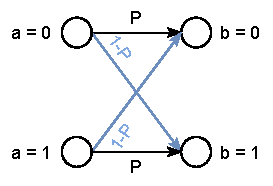
\includegraphics[scale = 1.2]{img/cbs.pdf}
  \caption{Rappresentazione di un canale binario simmetrico}
  \label{fig:cbs}
\end{figure}
Mi basta quindi solo il valore di $P$ per avere tutte le informazioni di un
CBS. \\
In un CBS ho quindi due simboli possibili in input e quindi, per praticità
chiamo: 
\[p(a=0)=p\]
\[p(a=1)=1-p\]
Ho quindi, lato equazioni di canale, che:
\[p(b=0)=p\cdot P+(1-p)\cdot (1-P)\]
\[p(b=1)=p\cdot (1-P)+ (1-p)\cdot P\]
Se avessi $P=1$ e $Q=0$ (ma anche $Q=1$ e $P=0$, avendo che sempre si ha
deterministicamente il cambio di bit) avrei un \textbf{CBS senza
  rumore}. Se avessi $P=\frac{1}{2}$ e $Q=\frac{1}{2}$ avrei un \textbf{CBS
  completamente rumoroso}.
Vedo anche le probabilità all'indietro, calcolabili con tutto quello di cui
abbiamo appena discusso:
\[P(a=0|b=0)=\frac{P(b=0|a=0)\cdot P(a=0)}{p(b=0)}=\frac{P\cdot p}{p\cdot
    P+(1-p)\cdot (1-P)}\]
Vediamo quindi i due casi particolari (facilmente verificabili sostituendo):
\begin{itemize}
  \item CBS senza rumore:
  \[P(a=0|b=0)=1\]
  \item CBS completamente rumoroso:
  \[P(a=0|b=0)=p\]
\end{itemize}
\[P(a=1|b=0)=\frac{P(b=0|a=1)\cdot P(a=1)}{p(b=0)}=\frac{(1-P)\cdot
    (1-p)}{p\cdot P+(1-p)\cdot (1-P)}\]
Vediamo quindi i due casi particolari:
\begin{itemize}
  \item CBS senza rumore:
  \[P(a=1|b=0)=0\]
  \item CBS completamente rumoroso:
  \[P(a=1|b=0)=1-p\]
\end{itemize}
\[P(a=0|b=1)=\frac{P(b=1|a=0)\cdot P(a=0)}{p(b=1)}=\frac{(1-P)\cdot p}{p\cdot
    (1-P)+ (1-p)\cdot P}\]  
Vediamo quindi i due casi particolari:
\begin{itemize}
  \item CBS senza rumore:
  \[P(a=1|b=0)=0\]
  \item CBS completamente rumoroso:
  \[P(a=1|b=0)=1-p\]
\end{itemize}
\[P(a=1|b=1)=\frac{P(b=1|a=1)\cdot P(a=1)}{p(b=1)}=\frac{P\cdot
    (1-p)}{p\cdot (1-P)+ (1-p)\cdot P}\]
Vediamo quindi i due casi particolari:
\begin{itemize}
  \item CBS senza rumore:
  \[P(a=1|b=1=1\]
  \item CBS completamente rumoroso:
  \[P(a=1|b=1)=p\]
\end{itemize}
\begin{esempio}
  Supponendo di avere un CBS con $P=\frac{9}{10}$, avendo che 9 volte su 10 il
  bit 
  arriva corretto. Si ha quindi $Q=\frac{1}{10}$, avendo progettato un ``buon
  canale'', anche se, senza sapere $p(a_i)$, il massimo che posso fare è
  supporli 
  uniformi. L'utente però potrebbe non usarlo per probabilità uniforme, ad
  esempio 
  qui suppongo un utente che inserisce secondo:
  \[P(a=0)=p=\frac{19}{20}\]
  \[P(a=1)=1-p=\frac{1}{20}\]
  Il ricevente vede uscire $b=0$ e vuole sapere se è entrato $a=0$:
  \[P(a=0|b=0)=\frac{171}{172}\]
  che sembra ragionevole. Si ha anche, ovviamente:
  \[P(a=1|b=0)=\frac{1}{172}\]
  Avendo che:
  \[P(a=0|b=0)>P(a=1|b=0)\]
  Si ha poi:
  \[P(a=0|b=1)=\frac{19}{28}\]
  \[P(a=1|b=1)=\frac{9}{28}\]
  Avendo che:
  \[P(a=0|b=1)>P(a=1|b=1)\]
  Ma allora se vede $b=1$ dice che comunque è più probabile $a=0$, non capendo
  quando sia entrato $a=1$.
\end{esempio}
Nell'esempio si è visto che le probabilità dipendono comunque dall'uso
dell'utente, che sceglie le $p(a_i)$, che se scelte male portano a situazioni
strane come quelle dell'esempio. Nell'esempio si è creato un bias che porta
sempre a scegliere $a=0$,avendo che $p(a=0)>>p(a=1)$. Questo succede in quanto,
guardando le equazioni sopra descritte, si ha, con questa scelta, $p>P$ e $p>Q$
(avendo indicato $p(a=0)$ con $p$).
\subsection{Entropie del Canale}
Dato un canale con $a_i\in A$ in input e $b_j\in B$ in output, con le varie
probabilità associate. Normalmente ho la sorgente $A$ di $q$ simboli, dove i
vari $P(a_i)$ sono una distribuzione di probabilità. Mettendosi 
nei panni di un osservatore che vede solo l'output si ha una ``sorgente'' $B$,
di $s$ simboli, dove i vari $P(b_j)$ sono una distribuzione di probabilità. La
vedo come sorgente perché il canale è una \textit{black box}, se invece potessi
vedere dentro vedrei che $B$ non sarebbe una sorgente, con le probabilità
$P(b_j)$ che non sono native ma derivate da quelle dei simboli $a_i$ e dalle
$P(b_j|a_i)$, tramite le equazioni di canale. \\
Si hanno molte entropie.\\
Posso dare l'entropia della sorgente $A$:
\[H_r(A)=\sum_{i=1}^q P(a_i)\cdot \log_r\frac{1}{P(a_i)}\]
Vedo $B$ come sorgente e quindi:
\[H_r(B)=\sum_{j=1}^s P(b_j)\cdot \log_r\frac{1}{P(b_j)}\]
Ho anche, ponendomi dal punto di chi vede sia $A$ che $B$, la quantità di
informazione media emessa dalla sorgente in input dato un simbolo in output:
\[H_r(A|b_j)=\sum_{i=1}^q P(a_i|b_j)\cdot \log_r\frac{1}{P(a_i|b_j)}\]
Questa è una sorta di \textbf{entropia tecnica} che serve a calcolare quella di
$A$ dato $B$:
\[H_r(A|B)=\sum_{j=1}^s P(b_j)\cdot H_r(A|b_j)\]
\[=\sum_{j=1}^s\sum_{i=1}^q P(b_j)\cdot p(a_i|b_j)\cdot
  \log_r\frac{1}{P(a_i|b_j)}\cdot \log_r\frac{1}{P(b_j)}\]
\[=\sum_{j=1}^s\sum_{i=1}^q P(a_i,b_j)\cdot \log_r\frac{1}{P(a_i|b_j)}\]
Questa è detta \textbf{equivocazione} e studia la quantità di informazione media
sull'input avendo in uscita un qualsiasi simbolo di $B$, essendo dal punto di
vista del ricevente che studia la quanittà di informazione immessa nel canale.\\
Si noti che si rompe quella sorta di simmetria nella formula dell'entropia (tra
il $P$ e il denominatore della frazione).\\
Un'altra entropia interessante è:
\[H_r(B|a_i)=\sum_{j=1}^s P(b_j|a_i)\cdot \log_r\frac{1}{P(b_j|a_i)}\]
Questa serve per l'altra entropia famosa che è:
\[H_r(B|A)=\sum_{i=1}^q\sum_{j=1}^s P(a_i,b_j)\log_r\frac{1}{P(b_j|a_i)}\]
Anche questa è detta \textbf{equivocazione} ed è la quantità di informazione
media sull'output avendo inserito un qualsiasi simbolo di $A$ nel canale,
essendo dal punto di vista del mittente che inserisce un simbolo qualsiasi nel
canale. 
Infine ho anche l'entropia congiunta:
\[H_R(A,B)=\sum_{i=1}^q\sum_{j=1}^s P(a_i,b_j)\log_r\frac{1}{P(b_j,a_i)}\]
Dove sono nel punto di vista di un osservatore esterno che vede input, canale e
output, qualunque sia il simbolo che entri nel canale e qualunque sia quello che
esca dal canale. \\
Suppongo che $A$ e $B$ siano indipendenti, ovvero che il canale è
\textit{completamente rumoroso}. Ma allora: 
\[P(a_i,b_j)=P(a_i)\cdot P(b_j)\]
E sostituendo:
\[H_r(A,B)=\sum_{i=1}^q\sum_{j=1}^s P(a_i)\cdot
  P(b_j)\log_r\frac{1}{P(a_i)\cdot P(b_j)}\]
\[=\sum_{i=1}^q\sum_{j=1}^s P(a_i)\cdot
  P(b_j)\cdot \left[\log_r\frac{1}{P(a_i)}+\log_r\frac{1}{P(b_j)}\right]\]
\[=\sum_{i=1}^q\sum_{j=1}^s P(a_i)\cdot
  P(b_j)\cdot \log_r\frac{1}{P(a_i)}+\sum_{i=1}^q\sum_{j=1}^s P(a_i)\cdot
  P(b_j)\cdot \log_r\frac{1}{P(b_j)}\]
Posso scambiare le sommatorie e portare fuori le cose che non dipendono più
dalle singole sommatorie, isolando ciò che riguarda $A$ e ciò che riguarda $B$,
ottenendo: 
\[=\sum_{j=1}^sp(b_j)\sum_{i=1}^qp(a_i)\cdot
  \log_r\frac{1}{P(a_i)}+\sum_{i=1}^qp(a_i)\sum_{j=1}^sp(b_j)\cdot
  \log_r\frac{1}{P(b_j)}\]
\[=H_r(A)\sum_{j=1}^sP(b_j)+H_r(B)\sum_{i=1}^qP(A_i)=H_r(A)+H_r(B)\]
Quindi:
\[H_r(A,B)=H_r(A)+H_r(B)\]

Avendo che le due sommatorie fanno 1.\\
E quindi se sono indipendenti la quantità di informazione congiunta è la somma
delle due singole quantità di informazione, avendo che la quantità di
informazione è additiva.\\
Si cerca una relazione tra la quantità di informazione in output e quella in
input, ipotizzando che un po' vada persa nel canale causi rumore. Sicuramente al
più in output avrò la stessa quantità di informazione. \\
Normalmente non si ha un canale completamente rumoroso quindi il simbolo in
output dipende da quello in input, avendo $A$ e $B$ non indipendenti ma si ha:
\[P(a_i,b_j)=P(a_i)\cdot P(b_j|a_i)\]
usando le probabilità in avanti che ho già a disposizione. Si ottiene quindi:
\[H_r(A,B)=\sum_{i=1}^q\sum_{j=1}^s P(a_i,b_j)\log_r\left[\frac{1}{P(a_i)}\cdot
    \frac{1}{P(b_j|a_i)}\right]\]
\[=\sum_{i=1}^q\sum_{j=1}^s
  P(a_i,b_j)\log_r\frac{1}{P(a_i)}+\sum_{i=1}^q\sum_{j=1}^s
  P(a_i,b_j)\log_r\frac{1}{P(b_j|a_i)}\]
Per la proprietà marginale so che:
\[\sum_{j=1}^s P(a_i,b_j)=P(a_i)\]
So anche che la seconda somma è l'equivocazione.\\
Ma allora:
\[H_r(A,B)=\sum_{i=1}^s P(a_i)\cdot \log\frac{1}{P(a_i)}+H_r(B|A)\]
Quindi in generale si ha, avendo che il primo termine della somma è l'entropia
di $A$:
\[H_r(A,B)=H_r(A)+H_r(B|A)\]
In caso fossero indipendenti avrei:
\[H_r(B|A)=H_r(B)\]
Ritrovando anche, qualora $A$ e $B$ fossero indipendenti:
\[H_r(A,B)=H_r(A)+H_r(B)\]
\subsection{Mutua Informazione}
\begin{definizione}
  Definiamo \textbf{mutua informazione} come la differenza di quantità di
  informazione data dal conoscere o non conoscere il simbolo in output dal
  canale:
  \[I(a_i;b_j)=\log_r \frac{1}{P(a_i)}-\log_r\frac{1}{P(a_i|b_j)}\]
  Ma quindi, per le proprietà dei logaritmi:
  \[I(a_i;b_j)=\log_r\frac{P(a_i|b_j)}{P(a_i)}\]
  Moltiplico sopra e sotto per $P(b_j)$:
  \[I(a_i;b_j)=\log_r\frac{P(a_i|b_j)\cdot P(b_j)}{P(a_i)\cdot P(b_j)}\]
  ma allora:
  \[I(a_i;b_j)=\log_r\frac{P(a_i,b_j)}{P(a_i)\cdot P(b_j)}\]
  E quindi:
  \[I(a_i;b_j)=\log_r\frac{P(b_j|a_i)\cdot P(a_i)}{P(a_i)\cdot P(b_j)}\]
  e infine:
  \[I(a_i;b_j)=\log_r\frac{P(b_j|a_i)}{P(b_j)}=I(b_j;a_i)\]
  Avendo che la mutua informazione quindi non dipende dall'ordine.\\
  Se considero il caso particolare in cui $a_i$ e $b_j$ sono indipendenti allora:
  \[P(a_i,b_j)=P(a_i)\cdot P(b_j)\]
  Allora:
  \[I(a_i;b_j)=\log_r\frac{P(a_i)\cdot P(b_j)}{P(a_i)\cdot P(b_j)}=0\]
  \textbf{Per ora si parla di un solo simbolo in input e uno solo in output}.\\
  Estendo la definizione alle medie:
  \[I(A;b_j)=\sum_{i=1}^q P(a_i|b_j)\cdot I(a_i;b_j)\]
  \[=\sum_{i=1}^q P(a_i|b_j)\cdot\log_r\frac{P(a_i|b_j)}{P(a_i)}\]
  E poi, per $B$:
  \[I(a_i;B)=\sum_{j=1}^s P(a_i|b_j)\cdot I(a_i;b_j)\]
  \[=\sum_{i=1}^q P(b_j|a_i)\cdot\log_r\frac{P(b_j|a_i)}{P(b_j)}\]
  e, come ultimo, la \textbf{mutua informazione del sistema}:
  \[I(A;B)=\sum_{i=1}^q P(a_i) I(a_i;B)\]
  \[=\sum_{i=1}^q\sum_{j=1}^s P(a_i,b_j)\log_r\frac{P(a_i,b_j)}{P(a_i)\cdot
      P(b_j)}=I(B;A)\]
\end{definizione}
\begin{teorema}
  Si può dimostrare che:
  \begin{itemize}
    \item $I(A;B)\geq 0$, per Gibbs
    \item $I(A;B)=0$ sse $A$ e $B$ sono indipendenti
    \item $I(A;B)=I(B;A)$
  \end{itemize}
\end{teorema}
La quantità di informazione trasmessa nel canale, per una distribuzione $P(a_i)$
fissata è proprio la mutua informazione del sistema. Infatti, tralasciando la
$r$ dell'entropia in quanto irrilevante:
\[I(A;B)=H(A)+H(B)-H(A,B)\]
e si sa che:
\[I(A;B)=H(A)+H(B)-H(A,B)\geq 0\]
Inoltre sappiamo che:
\[H_r(A,B)=H_r(A)+H_r(B|A)\]
\[H_r(A,B)=H_r(B)+H_r(A|B)\]
Uso una delle due per sostituire:
\[I(A;B)=H(A)-H(A|B)\geq 0\]
oppure:
\[I(A;B)=H(B)-H(B|A)\geq 0\]
Ma so quindi che (l'entropia è comunque $\geq 0$):
\[0\leq H(A|B)\leq H(A)\]
e che:
\[0\leq H(B|A)\leq H(B)\]
Scopro quindi che:
\[H(A,B)\leq H(A)+H(B)\]
e vale l'uguaglianza sse $A$ e $B$ sono indipendenti, avendo un canale
completamente rumoroso.\\
Tra tutte queste formule abbiamo come importanti:
\[I(A;B)=H(A)-H(A|B)\geq 0\]
che ci dice che la mutua informazione del sistema corrisponde a quella trasmessa
meno l'equivocazione, che altro non è che la quantità di informazione persa
causa rumore (\textit{non si dimostra la cosa}). Avere $I(A;B)\geq 0$ è data dal
fatto che il rumore non mi può mandare in negativo, ``togliendo più
dell'informazione presente''.\\
L'altra formula essenziale:
\[H(A,B)\leq H(A)+H(B)\]
Avendo che al più la massima informazione è la somma di quella di $A$ e di
quella di $B$, valore massimo che si ottiene solo se sono indipendenti. Negli
altri casi si ha l'intervento del rumore, vedendo uscire meno quantità di
informazione di quella entrata.
\subsection{Capacità del Canale}
Abbiamo detto che la quantità di informazione trasmessa nel canale, per una
distribuzione $P(a_i)$ fissata è proprio la mutua informazione del sistema. Ma
sappiamo che una scelta errata della distribuzione comporta cose inaspettate ed
errate. Si vuole evitare che l'utente faccia scelte inopportune e si vorrebbe
che 
la quantità di informazione trasmissibile dal canale non dipenda dalla scelta
dell'utente, la \textit{capacità del canale} non deve dipendere da $P(a_i)$.
\begin{definizione}
  Si definisce, informalmente, la \textbf{capacità del canale} $C$ come la
  massima 
  quantità di informazione trasmissibile dal canale (ovvero la mutua
  informazione del sistema) al variare di tutte le
  possibili $P(a_i)$: 
  \[C=\max_{P(a_i)}\,I(A;B)\]
\end{definizione}
Questa definizione è corretta matematicamente ma non aiuta dal punto di vista
pratico, dovendo calcolare tutte le:
\[I(A;B)=\sum_{i=1}^q\sum_{j=1}^s P(a_i,b_j)\log_r\frac{P(a_i,b_j)}{P(a_i)\cdot
    P(b_j)}\]
al variare dei $P(a_i)$.\\
Si sono quindi ricercate delle \textit{restrizioni} ragionevoli.\\
La principale di queste deriva dal fatto che:
\[I(A;B)=H_r(B)-H_r(B|A)\]
Ma allora:
\[I(A;B)=H_r(B)-\sum_{i=1}^q\sum_{j=1}^s P(a_i,b_j)\log_r\frac{1}{P(b_j|a_i)}\]
\[=H_r(B)-\sum_{i=1}^q\sum_{j=1}^sp(a_i)\cdot
  P(b_j|a_i)\log_r\frac{1}{P(b_j|a_i)}\]
\[H_r(B)\sum_{i=1}^q p(a_i)\cdot\sum_{j=1}^s
  P(b_j|a_i)\log_r\frac{1}{P(b_j|a_i)}\]
Quindi nella matrice di canale mi fisso su una riga, per $a_i$, e calcolo coi
valori della riga, variando per $b_j$.\\
Si è quindi pensato ad un \textbf{canale uniforme}, dove gli elementi di ogni
riga della matrice sono sempre gli stessi, al più di una permutazione. Ogni riga
è quindi una permutazione della prima riga. Posso ovviamente avere righe uguali.
Con un canale uniforme chiamo:
\[w=\sum_{j=1}^sP(b_j|a_i)\log_r\frac{1}{P(b_j|a_i)}\]
per una certa riga e quindi, per un canale uniforme:
\[I(A;B)=H_r(B)-\sum_{i=1}^q p(a_i)\cdot w\]
Ma $w$ non dipende da $i$:
\[I(A;B)=H_r(B)-w\cdot \sum_{i=1}^q p(a_i)\]
Ma quindi, avendo $\sum_{i=1}^q p(a_i)=1$:
\[I(A;B)=H_r(B)-w\]
Fare:
\[C=\max_{P(a_i)}\,I(A;B)\]
equivale quindi a:
\[C=\max_{P(a_i)}\,\{H_r(B)-w\}\]
ma $w$ è costante:
\[C=\max_{P(a_i)}\,\{H_r(B)\}-w\]
Vediamo se esistono tali canali uniformi.\\
Torniamo al CBS. Guardando la matrice vedo che la seconda riga è una
permutazione della prima e quindi il CBS è un canale uniforme.\\
Prendiamo ora l'n-esima estensione di un CBS, $CBS^n$, per $n\geq 1,
n\in\mathbb{N}$. In un $CBS^n$ ho n copie del CBS che trasmettono un bit con una
certa probabilità di trasmissione corretta, uguale per tutte. Con un $CBS^n$
posso trasmettere un pacchetto di $n$ bit, dove ogni bit ha la stessa
probabilità di trasmissione corretta $P$ ed errata $Q=1-P$. Ogni bit è
trasmesso indipendentemente dagli altri, un errore su un bit non influisce sulla
trasmissione degli altri. Questo ci riporta la \textbf{rumore bianco}, infatti
$CBS^n$ è il canale che si usa nel modello del canale bianco. La matrice di
$CBS^n$, per un certo $n$, è uniforme, avendo quindi un canale uniforme.\\
Abbiamo quindi già due canali uniformi: CBS e $CBS^n$. Ha senso quindi studiare
tali canali uniformi.\\
Calcolo ora la mutua informazione e la capacità del CBS.\\
Parto calcolando $w$ e scelgo di usare la prima riga, $[P\,\,\,Q]$:
\[w=P\log_2\frac{1}{P}+Q\log_2\frac{1}{Q}\]
e quindi, essendo $Q=1-P$:
\[w=P\log_2\frac{1}{P}+(1-P)\log_2\frac{1}{1-P}\]
oppure, avendo $P=1-Q$:
\[w=(1-Q)\log_2\frac{1}{1-Q}+Q\log_2\frac{1}{Q}\]
Ricordo che, vedere anche la figura \ref{fig:ber}:
\[H_2(p)=p\log_2\frac{1}{p}+(1-p)\log_2\frac{1}{1-p}\]
Ma allora, avendo qui $P=p$:
\begin{itemize}
  \item $w=H_2(P)$
  \item $w=H_2(Q)$
\end{itemize}
E mi basta sapere o $P$ o $Q$ avendo che sono legati. Per un CBS però $P$ è un
numero e basta, e anche $Q$ quindi:
\[C=\max \{H_2(B)-h_2(P)\}=\max \{H_2(B)\}-h_2(P)\]
\[C=\max \{H_2(B)-h_2(Q)\}=\max \{H_2(B)\}-h_2(Q)\]
In un BBS la distribuzione in input dipende solo da $p$, ricordando la figura
\ref{fig:cbs}, e quindi: 
\[C=\max_p \{H_2(B)\}-h_2(P)\]
\[C=\max_p \{H_2(B)\}-h_2(Q)\]
Si ha che $B$ corrisponde all'output, ovvero la sorgente che vede il
destinatario ed è comunque Bernoulliana e quindi è anche lei come la figura
\ref{fig:ber}. Se chiamo $x$ la possibilità che esca 0 e $1-x$ che esca 1. Posso
operare però solo su $p$ e il massimo di $h_2(B)$ è $\frac{x}{2}$ ma allora, per
le equazioni di canale:
\[x=p\cdot P+(1-p)\cdot (1-P)\]
\[=p\cdot P+1-P-p+p\cdot P\]
\[=1-P-p+2\cdot p\cdot P\]
\[=1-P-p\cdot (1-2\cdot P)\]
Cerco un $p$ che dia $x=\frac{1}{2}$:
\[\frac{1}{2}=x\]
\[=p(1-2\cdot P)=\frac{1}{2}-P=\frac{1-2\cdot P}{2}\]
Ma allora, dividendo il primo e l'ultimo termine:
\[p=\frac{1}{2}\]
Ma ho supposto:
\[1-\cdot P\neq 0\to P\neq \frac{1}{2}\]
che è ragionevole perché sarebbe un canale completamente rumoroso. Assumo quindi
un CBS non completamente rumoroso.\\
Posso quindi dire che:
\[C=1-H_2(P)\]
\[C=1-H_2(Q)\]
In quanto il valore massimo dell'entropia della Bernoulliana è 1 e la si ottiene
quando la probabilità di uscita vale $\frac{1}{2}$, che vale quando anche la
probabilità di inserire un valore è $\frac{1}{2}$ (??? risentire ultimi 15m
lezione 2 13 aprile).\\
Passando a $CBS^n$ ho che ogni singolo CBS è uguale e che la quantità di
informazione è additiva. Si ha quindi la capacità di un $CBS^n$:
\[C=n\cdot \left(1-H_2(P)\right)\]
\[C=n\cdot \left(1-H_2(Q)\right)\]
\section{Secondo Teorema di Shannon}
\textbf{La dimostrazione del teorema non viene fatta a lezione}.\\
Questo teorema è forndamentale nella teoria dell'informazione.\\
Con questo teorema si usa praticamente tutto quanto spiegato in questo
capitolo.\\
Si useranno alcuni passaggi matematici.\\
In primis la seguente maggiorazione, avendo $H(\cdot)$ funzione entropia per una
sorgente Bernoulliana: 
\[\sum_{k=0}^{\lambda \cdot n}\leq 2^{n\cdot
    H(\lambda)},\,\,\,0<\lambda<\frac{1}{2},\, \lambda\cdot n\in \mathbb{N}\]
Si ha poi il seguente teorema:
\begin{teorema}[Legge Debole dei Grandi Numeri]
  Date $x_1,\ldots X_n$ variabili casuali indipendenti, con stessa
  distribuzione, media $\mu$ e varianza $\sigma^2$ si ha che $\forall
  \varepsilon>0$ piccolo a piacere e $\forall\delta>0$, $\exists n_0$ tale che,
  $\forall n> n_0$:
  \[P\left(\left| \frac{1}{n}\sum_{i=1}^n X_i-\mu\right|\leq
      \varepsilon\right)\geq 1-\delta\]
  Ovvero, detto altrimenti:
  \[P\left(\left| \frac{1}{n}\sum_{i=1}^n X_i-\mu\right|>
      \varepsilon\right)<\delta\]
  Avendo che la media dei valori $X_i$ può essere portata, con alte probabilità,
  vicino quanto si vuole a $\mu$, che altro non è che il valore atteso. Si dice
  infatti che la media di tali valori dista da $\mu$ per un $\varepsilon>0$
  piccolo a piacere.
\end{teorema}
Ogni bit inviato forma l'insieme delle variabili casuali che descrivono i
risultati dei nostri $n$ ``esperimenti'' indipendenti e uguali. per il teorema
posso portare il valore medio di tale sequenza di esperimenti vicino al $\mu$ di
ogni esperimento (non con certezza ma con probabilità prossima quanto si vuole a
1).\\
Ci si aspetta quindi un errore medio pari a $n\cdot Q$ nella spedizione di $n$
cifre da un $CBS^n$ ma per tale teorema lo porteremo prossimo quanto si vuole a
$Q$, a patto di avere $n$ grande (spedendo quindi grandi sequenze di bit).\\
Il secondo teorema di Shannon, a differenza del primo, riguarda i \textbf{canali
  rumorosi}. 
\begin{teorema}[Secondo Teorema di Shannon]
  Dato un canale rumoroso, con una certa capacità $C$, è possibile trasmettere
  informazioni avvicinandosi arbitrariamente alla capacità del canale e
  contemporaneamente mantenendo arbitrariamente bassa la probabilità d'errore,
  ovvero la probabilità che il ricevente sbagli a decodificare. Si mantiene
  quindi l'affidabilità del canale, appunto la probabilità di ricevere
  correttamente i messaggi, prossima a 1.
\end{teorema}
\textbf{Su elearning dettagli della dimostrazione. Quanto detto in seguito è
  solo qualche commento non richiesto all'orale}.\\
La struttura della dimostrazione parte da un a definizione:
\begin{definizione}
  Definiamo \textbf{regola di decisione} come una funzione che usa il
  decodificatore per capire quale simbolo è stato spedito a partire dal simbolo
  ricevuto:
  \[d:B\to A\]
\end{definizione}
Si da per scontato che possa avvenire un errore. Si ha una matrice con le
probabilità all'indietro che mi dice le probabilità di avere un $a_i$ avendo
ricevuto $b_j$. Le colonne di tale matrici sommano 1 e hanno appunto le
\textbf{probabilità all'indietro} $P(b_j|a_i)$ e si usa una \textbf{regola di
  massima verosomiglianza}. Potrei anche avere equiprobabilità studiando tali
regole che quindi non sono uniche. \\
Si parla poi di \textbf{probabilità d'errore}, ovvero la probabilità che il
ricevente sbagli a decodificare, ovvero ricevuto $b_j$ non si capisca il giusto
$a_i$. \\
Il teorema poi si dimostra usando $CBS^n$ e assumendo rumore bianco, ma anche
per altri tipi di canale, che comportano conti più complessi.\\
Si suppone $Q<\frac{1}{2}$ anche perché se no avrei o un canale completamente
rumoroso, con $=$, o che ``sbaglia'' più di metà delle volte ma quindi, essendo
Bernoulliano, ha comunque $Q<\frac{1}{2}$.\\
Con $A$ assumo solo i messaggi validi:
\[A\subset\{0,1\}\]
Mentre $B$ sono tutti i possibili:
\[B\subseteq\{0,1\}\]
Inoltre, per il $CBS^n$:
\[P(a_i)=\frac{1}{m}\]
e quindi:
\[I(a_i)=\log_2\frac{1}{\frac{1}{n}}=\log_2 m\]
E si ha poi:
\[n\cdot C=n\cdot (1-H_2(Q))\]
Per il teorema, dato $\varepsilon_1>0$:
\[I(a_i)=\log_2 n=n\cdot (C-\varepsilon_1)\]
\[=n\cdot C-n\cdot \varepsilon_1\]
che dipende da $n$. Ma allora:
\[m=2^{n\cdot(C-\varepsilon_1)}=\frac{2^{n\cdot C}}{2^{n\cdot\varepsilon_1}}\]
Si scelgono poi casualmente i messaggi.\\
Ipotizzo una sfera per la correzione di raggio, in fase di invio per $a_i$,
per $\varepsilon_2>0$: 
\[r=n\cdot Q+\varepsilon_2\]
in modo che il destinatario, che anche lui ha una sfera per la correzione
d'errore e sceglie il simbolo più vicino al centro, che è il più probabile, che
equivale ad usare la massima verosimiglianza. Qualora però tale simbolo non
fosse univoco si avrebbe errore, avendo errore nella decisione (che è l'errore
della probabilità d'errore). Nemmeno provo a valutare altri simboli
equidistanti. Si calcola quindi la probabilità di commettere tale errore e si
continua con il ragionamento del teorema.\\
Shannon fa quindi una media di tutti i messaggi validi, ovvero su tutte le
codifiche casuali, facendo poi vari ragionamenti geometrici e applicando i due
costrutti matematici posti ad inizio sezione e la cosiddetta
\textbf{equazione di Fano}.\\
Si cerca di dimostrare anche \textbf{l'inverso del secondo teorema di Shannon},
mettendo nel canale più informazione di quella che è trasmissibile dal
canale. Si arriva a dire che, forzando il canale, la probabilità di errore non
può arrivare a 0, restando ad un valore comunque positivo, sbagliando quindi a
decodificare.\\ 
Il secondo teorema comunque ci dice che esiste il codice ma non ci dice come è
fatto ma si è 
visto che usando la codifica casuale spesso si ottiene qualcosa di
funzionante. \textbf{Ha comunque più valenza teorica che pratica}.
\chapter{Crittografia}
Lo scopo della \textbf{crittografia} è quello di memorizzare, trasmettere ed
elaborare informazioni, in presenza di agenti ostili, che voglio leggere e
modificare tali informazioni. La crittografia non è la \textbf{steganografia},
che consiste nel nascondere un messaggio dentro dati multimediali, occupandosi
quindi di impronte digitali etc$\ldots$\\
Con al crittografia non nascondo l'esistenza del messaggio ma lo codifico in
modo che un esterno non possa farci nulla. Tendenzialmente basta la
crittografia. \\
La crittografia è quindi una codifica, che si aggiunge alla codifica di
sorgente e alla codifica di canale, che limita la comprensione del contenuto al
mittente e al destinatario.\\
Ormai la crittografia è una scienza che comprende tante tematiche. Si hanno
quindi sia questioni di complessità computazionale, per cifrare e decifrare
(mittente e ricevente devono metterci pochissimo a cifrare e decifrare mentre
gli altri migliaia di anni). Si frutta quindi la \textbf{teoria dei numeri} e
l'\textbf{algebra}, con monoidi, campi, anelli etc$\ldots$ e la
\textbf{complessità computazionale}.\\
Le applicazioni della crittografia variano dallo storage ai DRM, dalle
criptovalute alla homomophic encryption, ovvero computazione fatta su dati
cifrati, dal cloud computing alla trasmissione sicura di dati sensibili e al
secure secret sharing, dove ogni partecipante ha una parte del segreto e servono
almeno $k$ partecipanti per ricostruirlo, con meno partecipanti non si ha
nemmeno una vaga idea dello stesso.\\
Lo schema standard sono \textbf{Alice} e \textbf{Bob} che si scambiano un
messaggio e \textbf{Eve} che cerca di intercettare il messaggio,
``origliando''. Alice e Bob comunicano su un canale pubblico. Eve può leggere
e/o scrivere sul canale, nel caso semplice solo leggere. Mandare il messaggio
\textit{msg} in 
chiaro, in plain text, viene sicuramente intercettato. Alice quindi codifica il
messaggio ma anche così facendo, senza ulteriori specifiche, Bob non sa come
leggere il messaggio. Bisogna quindi far dipendere la codifica da una chiave $k$
conosciuta solo da Alice e Bob. Alice calcola il $c$, ciphertext, come il
risultato della cifratura con $k$ e lo spedisce a Bob. Bob quindi, conoscendo la
chiave può riottenere il messaggio originale, tramite una funzione
$msg=D_k(c)$. Eve non sapendo $k$ non può fare nulla: $???=D_?(c)$.
Per Bob quindi decifrare è facile per Eve quasi impossibile.\\
In realtà la crittografia, che prevede lo studio e la progettazione di
crittosistemi sicuri, era chiamata \textbf{criptologia}. La
\textbf{crittoanalisi} studia invece come ``rompere'' i crittosistemi, portando
ad uno studio ``evolutivo'' dei sistemi. Quindi sia crittografia che
crittoanalisi sono importanti, anche perché Eve potrebbe essere la ``parte
buona'', come la polizia che intercetta i terroristi. Servono quindi entrambi
gli aspetti.\\
La criptologia era spesso definita l'unione di crittografia e crittoanalisi.\\
Parlando dell'\textbf{attaccante} Eve bisogna stabilire delle assunzioni, dando
un modello. Si ha quindi che:
\begin{itemize}
  \item se Eve non può né leggere né scrivere il canale è sicuro. È una
  situazione non realistica, avendo che normalmente si comunica via radio
  attraverso l'aria o via cavo
  \item se Eve può leggere ma non scrivere si hanno solo \textbf{attacchi
    passivi}, ovvero leggere i messaggi e trarne vantaggio, ed è
  la situazione più comune. Non si hanno \textbf{impersonificazioni}, ovvero far
  finta di essere uno dei due estremi della comunicazione, far finta di essere
  Bob o Alice
  \item se Eve può scrivere ma non leggere si ha che può disturbare la
  comunicazione, avendo che ogni canale ha, come visto, una capacità massima e
  se la superiamo, per il secondo teorema di Shannon, provochiamo errori di
  decodifica. Eve può quindi cercare di saturare il canale ma non riesce a
  trarre vantaggio dal messaggio, non potendolo leggere
  \item se Eve può leggere e scrivere si ha che può fare \textbf{attacchi
    attivi} e \textbf{impersonificazioni}. È la situazione ovviamente più
  pericolosa 
\end{itemize}
SI ha che:
\begin{itemize}
  \item Alice vuole mandare il plaintext $m$
  \item Alice codifica $m$ tramite una funzione $E(\cdot)$, ottenendo un
  ciphertext, $c=E(m)$ 
  \item Alice spedisce $c$
  \item Bob decodifica $c$ tramite $D(\cdot)$, $m=D(c)$
\end{itemize}
Alice e Bob devono quindi accordarsi prima sulle due funzioni, magari, a sua
volta, in un canale non sicuro. Le due funzioni $E$ e $D$ devono essere
mantenute segrete. Alice e Bob, più precisamente, si accordano sull'algoritmo di
cifratura e di conseguenza di decifratura. Già alla fine del 1800 Kerkhoff
enuncia il suo principio:
\begin{center}
  \textit{mantenere segrete le funzioni è difficile mentre mantenere segreta una
  piccola informazione come la chiave è più semplice.}
\end{center}
L'algoritmo quindi può anche essere pubblico ma senza la chiave non te ne fai
nulla. Inoltre cambiare chiave è più semplice che cambiare algoritmo.\\
Nella modernità gli algoritmi sono spesso opensource, garantendo ancora più
sicurezza tramite la community che lavora sull'algoritmo, evidenziando falle e
problematiche (cosa che garantisce anche una certa visibilità).\\
Le chiavi sono piccole, ad esempio 128, 192 o 256 bit per AES. Sono quindi più
facili da tenere nascoste rispetto ad intere procedure.\\
Se Eve scopre la chiave segreta rompe il crittosistema, e ogni messaggio diventa
praticamente in chiaro. IN tal caso si parla di \textbf{rotture
  totali}. Un'altra situazione è che Eve abbia varie copie $c$ (perché ``spia'')
e $m$ (visto che magari dopo un po' diventa pubblico), venendo a conoscenza
magari della relazione tra $c$ e $m$, si parla in caso di \textbf{rottura
  parziale}. Un messaggio cifrato può restare pubblico per un tot di tempo prima
che il rischio di essere decifrato diventi troppo alto. Questo tempo varia a
seconda dell'algoritmo, della chiave e dei possibili avversari (se si parla di
NSA auguri). Un'altra variabile nel discorso è quanto il messaggio deve rimanere
effettivamente segreto. Si ha inoltre una serie di assunzioni non dimostrate e
uno potrebbe trovare un modo per risolvere problemi che si credono
difficili. Un'altro aspetto è la \textbf{legge di Moore}, avendo che le macchine
con cui si decifra evolvono e si potenziano ogni circa 18 mesi. Si potrebbero
anche avere nuovi algoritmi etc$\ldots$ e magari un'informazione sicura ora non
lo sarà tra 100 anni, quando magari si avranno computer quantistici a pieno
regime (e quindi serviranno altri algoritmi di cifratura). Spesso si usano due
algoritmi in modo che, a medio termine, se un algoritmo viene rotto si usa
l'altro. 
\begin{definizione}
  Definiamo formalmente un \textbf{crittosistema} come una quintupla:
  \[(PT,CT,K, E(\cdot), D(\cdot))\]
  Dove:
  \begin{enumerate}
    \item $PT$, spazio dei plaintext, ovvero lo spazio di tutti i possibili
    testi in chiaro. Solitamente sono stringhe binarie quindi è un insieme
    $\{0,1\}^*$ o comunque un certo $\Sigma^*$ (nei cifrari storici e basta)
    \item $CT$, spazio dei ciphertext, mi piacerebbe fosse anch'esso $\{0,1\}^*$
    \item $K$, spazio delle chiavi, detto \textbf{keyspace}, ovvero i possibili
    valori che può assumere la chiave segreta. Il keyspace non deve essere
    troppo piccolo perché l'attaccante potrebbe usare il bruteforce
    \item funzione di cifratura $E:PT\times K\to CT$
    \item funzione di decifratura $D:CT\times K\to PT$
  \end{enumerate}
  Spesso si indicano $E_k(\cdot)$ anziché $E(\cdot, k)$ ed equivalente per
  $D$.\\
  Scegliendo $k\in K$ scelgo una coppia $E_k$ $D_k$. \\
  Si noti che:
  \[CT=\cup_{k\in K}E_k(PT)\]
  Si ha che:
  \[\forall m\forall k,\,\,D_k(E_k(m))=m\]
  Anche se non è vero in assoluto. Nei crittosistemi simmetrici si
  usa la stessa chiave per cifrare e decifrare, anche se in realtà si usa, per
  decifrare, una chiave \textbf{ottenibile} (e non per forza la stessa)
  facilmente da quella usata per 
  cifrare. \emph{Nell'equazione quindi si assume che la chiave sia proprio la
  stessa}.\\  
  Si ha che $\forall m$ e $\forall k$ $c=E_k(m)$ deve essere facile da computare
  ma deve essere (estremamente)
  difficile trovare $m$ conoscendo solo $c=E_k(m)$. Deve essere facile computare
  $m$ conoscendo $c$ e $k$ ma deve essere (estremamente) difficile trovare $K$
  sapendo solo $c=E_k(m)$ e $m$.
\end{definizione}
\begin{shaded}
  Facile e (estremamente) difficile sono in termini di complessità
  computazionale (computati o meno in tempo polinomiale da una DTM). Per altri
  modelli uso la \textbf{TM probabilistica} ma mai la NDTM, perché risolve in
  tempo polinomiale problemi che in pratica non sappiamo realmente risolvere in
  tempo polinomiale. 
\end{shaded}
Una macchina che effettua un attacco bruteforce capisce di aver trovato
la giusta chiave a seconda di vari aspetti. Dipende da cosa viene cifrato. Ad
esempio parlando di file lo si capisce guardando i primi byte, i metadati, e
se sono consistenti con il formato che ci si aspetta si è arrivati alla giusta
decodifica. Se si parla di un semplice file di testo o si guarda se ci sono
parole riconoscibili tramite un dizionario o guardare l'entropia del messaggio
ottenuto, visto che i messaggi in linguaggio naturale sono molto ridondanti,
avendo quindi ridondanza bassa. Se la decifratura non va a buon fine ottengo un
risultato pseudo casuale, simile al risultato di una cifratura. L'entropia basta
anche solo di un pezzo.\\
Fare i controlli dopo una cifratura non è un grosso problema, sono calcoli
veloci. Quindi aumentando lo spazio delle chiavi si aumenta la complessità,
visto che il singolo controllo non è difficile.
\section{Cifrari Storici}
Partiamo con qualche accenno storico per capire il discorso.
\subsection{Cifrario di Cesare}
Tra \textbf{cifrari storici} abbiamo il \textbf{cifrario di Cesare}, che è un
crittosistema simmetrico molto debole (ma in un periodo dove ben pochi sapevano
anche solo leggere andava più che bene). Il messaggio, si narra, era scritto
sulla testa di uno schiavo dopo averlo rasato, aspettando che poi crescessero i
capelli prima di mandarlo al destinatario. Si hanno:
\begin{itemize}
  \item $\Sigma=\{A,B,\ldots, Z\}$
  \item $PT=CT=\Sigma^*$
  \item $K=\{1,2,\ldots,25\}$
  \item ogni lettera è cifrata e decifrata indipendentemente
\end{itemize}
Nella cifratura, fissata $k$, si ottiene $c$ avanzando di $k$ posizioni ogni
lettera nell'alfabeto. Per decifrare si ``torna indietro'' di $k$ posizioni
sull'alfabeto, eventualmente iniziando da capo, in modo circolare. Per questo
$k=0$ non ha senso e si parte da $k=1$.\\ 
Avanzare di 25 posizioni equivale a tornare indietro di una. Il problema è
quindi il keyspace piccolissimo (e Olivio disse che Cesare usasse sempre
$k=3$).\\
Il cifrario di Cesare è un esempio di \textbf{crittosistema per sostituzione
  monoalfabetica}, in quanto ogni lettera, fissato $k$, è sempre sostituita con
la stessa (e anche questo è un problema di sicurezza).\\
Si hanno altre caratteristiche interessanti:
\begin{itemize}
  \item decifrare con $k$ equivale a cifrare con $26-k$
  \item $D_kE_k=E_0D_0$
  \item posso riordinare passi di cifratura e decifratura ottenere lo stesso
  risultato 
\end{itemize}
\subsection{Crittosistema di Hill}
Un altro sistema storico è il \textbf{crittosistema di Hill}. In questo caso non
si ha più sostituzione monoalfabetica e fa uso dell'algebra lineare. Resta
comunque poco sicuro evidenziando una ``bad practice'', ovvero fa tutto tramite
operazioni lineari. È un crittosistema simmetrico con la chiave di decifratura
che è la matrice inversa di quella di cifratura (non uso la stessa chiave
quindi). Fare l'inversa di una matrice è un \textbf{problema facile} e quindi è
comunque un crittosistema simmetrico.\\
Si hanno come chiavi i numeri da 0 a 25 che rappresentano le lettere
dell'alfabeto (la a è 0 etc$\ldots$). Ogni operazione è fatta in
$\bmod\,\,26$. Si sceglie un intero 
$d\geq 2$ e si cifrano blocchi di $d$ lettere. Si cifra un blocco alla volta e
non una lettera alla volta. La chiave di cifratura è una
matrice quadrata $M$, con valori da 0 a 25, tale che, se $\det(M)\neq 0$ allora
la matrice è invertibile e l'inversa ha valori tra 0 e 25. Ad esempio:
\[M=\left[
    \begin{matrix}
      3 & 3\\
      2 & 5
    \end{matrix}
  \right]\to M^{-1}=\left[
    \begin{matrix}
      15 & 17\\
      20 & 9
    \end{matrix}
  \right]
\]
Per vedere se la matrice è invertibile si guarda il determinante.\\
La chiave per decifrare non è quindi la chiave per cifrare ma si ottiene
facilmente da essa.\\
I $d$ numeri (che rappresentano le lettere) si mettono un vettore e si sceglie
quindi la matrice che funge da chiave per cifrare. \\
Si avrà che $PT=CT$. Divido il testo $m$ in $l$ blocchi $P_i$ di $d$ lettere e
se la lunghezza di $m$ non è un multiplo di $d$ si aggiungono a $m$ lettere
fittizie che siano riconoscibili come tali (anche se questa cosa può anche
aiutare l'attaccante). Si avrà quindi:
\[m=P_1P_2\ldots P_l\]
Si ha quindi che ogni blocco viene cifrato a parte:
\[C_i=M\cdot P_i,\,\,\,\forall i =1,2,\ldots, l\]
Moltiplicando la matrice per il vettore ottengo un altro vettore, coi numeri che
corrispondono le lettere del blocco cifrate.\\
e infine si concatenano i $C_i$ per ottenere il testo cifrato:
\[c=C_1C_1\ldots C_l\]
\begin{esempio}
  Si ha $m=HELP$ e $d=2$. Come chiavi uso:
  \[M=\left[
      \begin{matrix}
        3 & 3\\
        2 & 5
      \end{matrix}
    \right]\to M^{-1}=\left[
      \begin{matrix}
        15 & 17\\
        20 & 9
      \end{matrix}
    \right]
  \]
  Si hanno quindi:
  \[P_1=
    \left[
      \begin{matrix}
        H\\
        E
      \end{matrix}
    \right]=\left[
      \begin{matrix}
        7\\
        4
      \end{matrix}
    \right]\mbox{ e }
    P_2=\left[
      \begin{matrix}
        L\\
        P
      \end{matrix}
    \right]=\left[
      \begin{matrix}
        11\\
        15
      \end{matrix}
    \right]
  \]
  Ma allora (ricordando le operazioni $\bmod \,\,26$):
  \[C_1=M\cdot P_1=\left[
      \begin{matrix}
        3 & 3\\
        2 & 5
      \end{matrix}
    \right]\cdot\left[
      \begin{matrix}
        7\\
        4
      \end{matrix}
    \right]=\left[
      \begin{matrix}
        7\\
        8
      \end{matrix}
    \right]\left[
      \begin{matrix}
        H\\
        I
      \end{matrix}
    \right]\]
  \[C_2=M\cdot P_2=\left[
      \begin{matrix}
        3 & 3\\
        2 & 5
      \end{matrix}
    \right]\cdot\left[
      \begin{matrix}
        11\\
        15
      \end{matrix}
    \right]=\left[
      \begin{matrix}
        0\\
        19
      \end{matrix}
    \right]\left[
      \begin{matrix}
        A\\
        T
      \end{matrix}
    \right]\]
  e quindi:
  \[c=C_1C_2=HIAT\]
\end{esempio}
Vediamo quindi se questo crittosistema è sicuro. Supponiamo che Eve sa o scopre
quanto valga $d$ (magari provandone tante, non è una cosa costosa
computazionalmente) ma non sa quanto vale $M$. Suppongo che veda passare $c$ e
che scopra $m$,
magari perché dopo un tot di tempo $m$ diventi pubblico o perché ha fatto
attività di intelligence. A questo punto Eve conosce anche i blocchi e i vettori
corrispondenti a $m$. Si ha quindi un semplice sistema di equazioni e se è
fortunata ottenendo una matrice invertibile allora può riottenere la chiave $M$
tramite semplici operazioni algebriche. Questo attacco è ancora più semplice se
Eve può scegliere il testo in chiaro, qualora l'algoritmo di cifratura sia
pubblico. \\
Se ottiene una matrice non invertibile si ha che ha ottenuto alcuni blocchi
dipendenti ma comunque potrebbe ricostruire una parte di matrice e, prima o poi,
magari scoprendo un altro pezzo del testo in chiaro, può scoprire l'intera
chiave $M$. \\
Il grosso problema è quindi che la cifratura è un'operazione lineare, essendo
fatta moltiplicando una matrice per un vettore. Si è quindi visto come un
crittosistema con operazioni lineari sia da evitare.
\subsection{Crittosistema di Playfair}
Nel 1854 si è pensato al \textbf{crittosistema di Playfair} che nella versione
base prevede addirittura una chiave fissa, ovvero una matrice $5\times 5$ di
lettere (non potendo cifrare la $j$ visto che in inglese si hanno 26
lettere). Il testo è diviso in blocchi di due lettere ma non posso avere blocchi
con due lettere uguali all'interno.\\
Si ha che la chiave è:
\[k=\left[
    \begin{matrix}
      s & y & d & w & z\\
      r & i & p & u & l\\
      h & c & a & x & f\\
      t & n & o & g & e\\
      b & k & m & q & v
    \end{matrix}
  \right]\]
Lo studio viene poi fatto in base a come sono le due lettere nella matrice, se
nella stessa riga/colonna muovendosi ciclicamente nella riga e nella colonna. Se
non sono nella stessa riga/colonna si identifica 
il sottorettangolo con le due lettere come estremi prendendo poi gli altri due
estremi. La decifratura si fa con le operazioni nell'ordine inverso.\\
Il problema grave è che la chiave è sempre la stessa. Per costruire altre chiavi
si parte da una frase, si tolgono le ripetizioni e si completa la sequenza
ottenuta con le lettere mancanti, in ordine alfabetico. Questo comporta un
inizio spesso di senso compiuto e una fine composta spesso dalle ultime lettere
dell'alfabeto (per il modo in cui la matrice viene creata a partire da una
frase, all'inizio la frase non viene quasi toccata ma alla fine si aggiungono
le ultime lettere dell'alfabeto, spesso poco frequenti).\\
\begin{esempio}
  Parto da:
  \begin{center}
    \textit{course on cryptography}
  \end{center}
  rimuovo le ripetizioni:
  \begin{center}
    \textit{coursenyptgah}
  \end{center}
  completo con le lettere mancanti tranne ``j'':
  \begin{center}
    \textit{coursenyptgahbdfiklmqvwxz}
  \end{center}
  Avrei la matrice:
  \[k=\left[
    \begin{matrix}
      c & o & u & r & s\\
      e & n & y & p & t\\
      g & a & h & b & d\\
      f & i & k & l & m\\
      q & v & q & x & z
    \end{matrix}
  \right]
\]
Ottenendo qualcosa di facile da analizzare.
\end{esempio}
È un sistema quindi polialfabetico ma le sostituzioni dei blocchi sono sempre le
stesse.
\subsection{Cifrario di Vigenère}
In realtà, nel 1586, fu creato il \textbf{cifrario di Vigenère}, che è stato
ritenuto sicuro per secoli.\\
Funziona circa come il cifrario di Cesare ma diventa abbastanza robusto in
quanto la chiave cambia dopo ogni cifratura di ogni lettera del plain. Per
cifrare e decifrare si usa una tabella contenente tutte le possibili cifrature
di Cesare. In altri termini si ha una tabella quadrata di righe e colonne apri
al numero delle lettere dell'alfabeto. La prima riga è nell'ordine giusto, la
secondo ruotata di 1 (si parte da ``b'' e si arriva ad ``a ``) e così via.\\
Come chiave si sceglie una parola che viene ripetuta fino a ottenere la stessa
lunghezza del testo in chiaro.\\
Si prende la coppia $(m_i,k_i$) e si usano queste come coordinate (la prima
colonna e la prima riga sono l'alfabeto in ordine coretto e si usano come
coordinate) per prendere una lettera dalla tabella sopra costruita. Per
decifrare si fa l'ordine opposto, partendo da $(c_i, k_i$), sfruttando la
colonna che inizia con $c_i$ cercando la cella contente $k_i$ per ottenere la
coordinata sulle righe.\\
Questo sistema è stato considerato sicuro al 100\% per secoli.\\
Si ha quindi che la i-esima lettera di $m$ è cifrata con il cifrario Cesare dove
la chiave è l'i-esima lettera di $k$.
Se la lunghezza di $k$ è $l$ (prima delle ripetizione) allora la lettera di $m$
in posizione $i$, $i+l$, $i+2\cdot l$ etc$\ldots$ sono cifrate sempre con lo
stesso carattere di $k$, quindi con la stessa chiave. Suppongo però di conoscere
la lunghezza della chiave e scrivo il testo cifrato in una matrice, di $k$
colonne, in modo che i caratteri cifrati dallo stesso carattere sono sulla
stessa colonna. Posso quindi fare un'analisi delle frequenze su ogni colonna e
trovare la chiave di ogni colonna. Si rompe quindi il crittosistema anche se il
numero di possibili chiavi di per $n$ lettere è $26^n$ (già solo per $n=5$
parliamo di $26^5=11881376$) essendo quindi un numero abbastanza grande per
rendere infattibile un bruteforce (a meno di usare un computer, cosa non
fattibile fino a qualche decennio fa). Bisogna comunque sapere la lunghezza
della chiave.\\
Nel 1860 Kasiski dice che se la chiave è lunga $n$ allora potrebbe capitare, se
$m$ ha certe regolarità, che la stessa parola potrebbe venire cifrata con la
stessa sequenza di chiavi. Si ottengono così, nel ciphertext, ripetizioni
lunghe $n$ di lettere (anche se comunque potrebbe essere un caso). Si può quindi
pensare che la chiave sia lunga quanto un divisore della distanza tra queste
ripetizioni (e per senso logico si estraggono un paio di valori possibili). SI
può quindi passare alla'analisi delle frequenze essendo comunque risolto
facilmente, in certi casi, lo step di trovare la lunghezza della chiave.\\
Può convenire, in questo caso, fare sovracifrature, ovvero cifrare i testi
cifrati etc$\ldots$ 
\subsection{Sicurezza dei Crittosistemi Storici}
Fino alla prima guerra mondiale anche crittosistemi deboli andavano bene causa
analfabetismo. Il crittosistema veniva fatto a mano, si cifrava a mano e si
trasmetteva in qualche modo. Non si potevano quindi fare troppe operazioni,
dovendo farlo a mano e spesso in guerra. Inoltre essendo fatto da un umano
doveva essere semplice per ridurre errori umani, che dovevano seguire le
istruzioni per cifrare.\\
In tempo di pace, all'inizio del 1900 si sono diffuse macchine meccaniche di
calcolo (prima enormi e poi sempre più piccole grazie alla corrente
elettrica). Si è quindi automatizzata la cifratura permettendo crittosistemi
arbitrariamente complessi (non essendoci più l'umano) con centinaia di
operazioni anche perché le macchine vengono usate anche per la crittoanalisi.
Tali macchine vengono create con obiettivi pacifici per usi aziendali (per
segreti aziendali, per la Borsa etc$\ldots$) e non bellici. Il mondo però
aziendale ha sdegnato questi macchinari che sono stati ``rispolverati'' in
ambito bellico, soprattutto durante la seconda guerra mondiale.\\
Tali macchinari utilizzano dei rotori (in sequenza il precedente al termine fa
scattare il successivo etc$\ldots$). Ogni rotore è diviso in celle e ogni cella
contiene una lettera. Ogni rotore effettua una sostituzione monoalfabetica e
ogni lettera di $m$ è cifrata usando tutti i rotori. La chiave è rappresentata
quindi dalla posizione dei rotori. Ogni volta che si cifra una
lettera il rotore più veloce scatta cambiando chiave. Con 26 lettere dopo $26^3$
lettere si ripresenta una ripetizione per la stessa lettera, rompendo ogni
analisi statistica. Il metodo per inserire il messaggio deve comunque essere
semplice. Si deve anche avere un modo comodo per vedere il messaggio cifrato.\\
Si passa quindi da macchine meccaniche a macchine elettro-meccaniche, con
collegamenti elettrici (26, uno per lettera) nei rotori, avendo che ogni rotore
implementa una permutazione fissata, cambiando sempre una lettera in
un'altra. Ad ogni rotazione cambia la coppia di lettere, ogni volta si ha quindi
una permutazione diversa.\\
\textbf{Immagini utili su slide}.\\
Si fa quindi una sostituzione polialfabetica con chiavi lunghissime, avendo che
la chiave iniziale è la posizione causale dei rotori all'inizio, da cui si
ottengono le varie chiavi derivate, dopo $26^n$ posizioni per $n$ rotori. Ogni
analisi statistica è destinata a fallire.\\
La \textbf{macchina Enigma} è ancora più complessa. Grande poco più di una
macchina da scrivere ha gli stessi tasti, in modo che si possa inserire
facilmente $m$. Si hanno di base 3 rotori (ma poi sono aumentati), con per di
più possibilità di 
cambiarli con altri rotori. Si sceglieva la posizione iniziale dei rotori e dopo
ogni lettera si accendeva una lampadina corrispondente alla lettera
cifrata. Faceva parte della chiave iniziale anche uno \textbf{scambiatore}, che
costituiva una ulteriore permutazione fissa (\textbf{immagini su slide}). La
cifratura faceva inoltre due giri sui rotori. La
macchina andava a batteria e durava un'intera giornata. \\
Decifrare a mano era letteralmente impossibile. I polacchi hanno iniziato per
primi a lavorare a come funzionassero le macchine Enigma per capire come
intercettare i nazisti. Anche gli inglesi le hanno studiate, capendo come
annullare l'effetto degli scambiatori, che per di più obbligavano una lettera a
non essere mai cifrata con se stessa.\\
Non si poteva comunque lavorare a mano e quindi Alan Turing costruì i macchinari
per decifrare. Tali macchinari erano delle \textbf{bombe logiche} e facevano
attacchi bruteforce (facendo molto casino a livello di rumore sonoro per di
più) tentando più chiavi in contemporanea, sapendo testo in chiaro e testo
cifrato. Se la chiave non andava bene scattava alla seguente producendo appunto
un suono simile al ticchettio di una bomba.\\
In merito si torna al discorso di quanto tempo può restare cifrato un messaggio
e avendo dietro gli Alleati che pagavano per costruire macchine per decifrare
tale tempo era alla fine poco.\\
C'era anche il macchinario detto \textbf{Colossus}, con la stessa potenza di un
Pentium 4, dedicato solo a studiare il keyspace.
\subsection{Crittoanalisi per Crittosistemi Storici}
Si possono in generale avere quattro scenari di attacco, in ordine di vantaggio
crescente per Eve:
\begin{enumerate}
  \item Eve conosce solo $x$ e vuole ottenere $m$. È una situazione tanto
  complicata per l'attaccante quanto rara. Si parla di \textbf{cryptotext only}
  \item Eve conosce alcune coppie $c_i,m_i$. Eve quindi studia i nuovi $c$ che
  arrivano e cerca di calcolare il corrispondente $m$. Si parla di \textbf{known
  plaintext}
  \item Eve può scegliere i testi in chiaro e computare i corrispondenti
  $c$. Eve quindi cerca di computare $m$ all'arrivo di un nuovo $c$. Durante la
  seconda guerra mondiale succedeva quando i tedeschi usavano per un giorno
  sempre la stessa chiave. È, modernamente, lo
  scenario classico della crittografia a chiave pubblica e si parla di
  \textbf{chosen plaintext} 
  \item Eve può decifrare ogni testo, scelto in modo adattivo, per un certo
  periodo di tempo. A questo Eve può più facilmente scoprire $m$ all'arrivo di
  un $c$. Si parla di \textbf{chosen ciphertext} 
\end{enumerate}
Si hanno quindi, in una piccola \textit{tassonometria} dei sistemi:
\begin{itemize}
  \item crittosistemi a chiave pubblica
  \item crittosistemi simmetrici che usano due operazioni fondamentali:
  \begin{enumerate}
    \item \textbf{trasposizione}, usando la chiave segreta come permutazione,
    all'aumentare della lunghezza dei blocchi permutati possono essere sicuri ma
    aumenta anche la complessità di calcolo. Si fa una sorta di
    anagramma. Questi crittosistemi non sono tendenzialmente sicuri
    \item \textbf{sostituzione}, come in Cesare. A loro volta si parla di
    sostituzioni \textbf{monoalfabetiche} o \textbf{polialfabetiche}, avendo che
    una stessa lettera può essere cifrata in modo diverso. Quest'ultima
    differenza è comunque molto relativa all'alfabeto in uso (si pensi ad Hill
    che diventa monoalfabetico nell'alfabeto dei blocchi, un blocco uguale
    diventa sempre lo stesso altro blocco). Monoalfabetici non sono sicuri ma
    nemmeno polialfabetici a meno di sostituzioni complesse
  \end{enumerate}
  Quindi un crittosistema simmetrico è una applicazione sequenziale di
  trasposizioni e sostituzioni a seconda di una chiave
\end{itemize}
Il crittosistema deve essere sicuro ma anche ``semplice'' da usare per
l'utente.\\
In un crittosistema per sostituzione monoalfabetico non si ha sicurezza in
quanto non si 
nascondono le proprietà statistiche delle lettere del testo in chiaro in
linguaggio naturale (in inglese, ad esempio, la lettera ``e'' compare più spesso
delle altre etc$\ldots$). Mi basterebbe quindi, statisticamente, sfruttare tali
percentuali, cercando la lettera più frequente nel ciphertext per supporre poi
che sia la ``e'' etc$\ldots$ Si hanno inoltre coppie (ma anche sulle terne) di
lettere ad alta frequenza e questo rendere ancora più debole il
crittosistema. Per tutte queste statistiche si hanno tabelle dedicate. Si può
cercare di falsare questi dati scrivendo testi su misura (con frasi non
convenzionali, ovviamente l'assenza di spazi etc$\ldots$) ma è abbastanza
difficile ottenere un risultato accettabile, se non impossibile (bastano pochi
tentativi per capire la corrispondenza tra caratteri o tuple di
caratteri). Questo succede appunto perché anche cambiando la lettera non
cambiano le frequenze della lingua sottostante (e anche se questa non si conosce
non sono così tante da rendere difficile andare a tentativi, inoltre lingue
simili hanno percentuali simili per i caratteri). Si può cercare di rendere
complicata la lingua usando lingue complesse e poco usate ma anche questa
operazione è difficile abbia successo (un esempio di uso erano gli americani
nella seconda guerra mondiale che usavano l'indiano Navajo)\\
Per risolvere il problema si sono usate varie possibilità. Ad esempio inserire
lettere extra rispetto al testo per falsare le frequenze, in modo che ogni
lettera abbia una frequenza simile alle altre.\\
Una tecnica che funziona molto bene è quella delle \textbf{omofone}. Si
supponga in uso l'alfabeto inglese. Sappiamo che ``e'' è la lettera più
frequente. Supponiamo quindi di usare un alfabeto $\Gamma=\{0,\ldots,99\}$ e se
una lettera appare il 12\% delle volte uso 12 numeri da $\Gamma$ e ogni volta
che ne vedo una scelgo uno di questi 12 numeri a caso. Si ottiene quindi una
\textbf{cifratura randomizzata}. La scelta può anche essere fatta con cura per
appiattire le frequenze delle omofone. Con le omofone la crittoanalisi diventa
complessa.\\
Se ogni volta scelgo a caso uno degli omofoni significa che lo stesso testo,
cifrato due volte in tempi diversi, porta a due ciphertext diversi. Lo stesso
testo in chiaro ha quindi sempre in ciphertext diverso ma questo non ha problemi
in fase di decifratura, nel momento in cui conosco le omofone. La decifratura
resta deterministica ma la cifratura diventa comunque più robusta.
\section{Crittosistemi Standard}
Nei tempi moderni, in ambito bancario, si è cercato ad un modo sicuro per
trasportare tra banche i registri con le cifre rappresentati i soldi. Ovviamente
tali registri devono essere sicuri.\\
Fino agli anni settanta ogni banca usava il proprio crittosistema, venduti da
aziende con annesso hardware. Se due banche dovevano comunicare dovevano
scegliere lo stesso.\\
Si inizia a pensare ad un crittosistema standard buono per usi civili, come
quelli bancari, ma anche non così buono per fini militari. Parte una ``gara''
per fare questo crittosistema standard. Negli USA c'era IBM che nel 1977
sviluppa \textbf{DES}, grazie ad un gruppo di ricerca tra cui
Feistel. All'inizio il crittosistema creato fu \textbf{Lucifer}, che venne però
considerato eccessivo, rallentando inutilmente onerosi i calcoli per l'hardware
dell'epoca (oltre alla volontà di indebolirlo per scopi civili da parte del
governo). L'NSA aveva avuto da dire anche sulle \textbf{s-box} di DES, ovvero le
parti 
non lineari, in quanto a conoscenza di sistemi non pubblici in grado di
romperle. DES usa chiavi a 56 bit, che a breve sarebbero diventate poche.\\
Si fa quindi una nuova ``gara'' che viene vinta da Daeman e Rijmen che creano
\textbf{AES}, con chiave da 128, 192 e 256 bit. AES verrà rotto dai computer
quantistici, è solo questione di tempo. Abbandoneremo quindi molti crittosistemi
attuali ma se ne hanno altri che resistono ai computer quantistici.
\subsection{DES}
\textbf{Non chiesti all'orale i dettagli, su slide ci sono le matrici e le
  varie tabelle}.\\
La chiave è lunga 56 bit avendo quindi un keyspace di $2^{56}$, che ora come ora
sono pochi. Questi 56 bit hanno un bit di parità ogni 7, in modo che ogni byte
sia dispari, che è un pasticcio inutile. Sono quindi 56 bit più 8 di parità, che
sono dipendenti.\\
DES fa iterazioni con una \textit{round function} su blocchi di 64 bit di $m$
per ottenere un $c$ di 54 bit. Ad ogni iterazione usa una chiave derivata
diversa calcolata dai 56 bit della chiave iniziale. Si ha che il calcolo delle
chiavi derivate è:
\begin{itemize}
  \item si riceve il pacchetto di 64 bit di $m$
  \item applico la permutazione iniziale, accedendo ai singoli bit della chiave
  e ai singoli bit di $m$. La permutazione è una matrice $8\times 8$
  \item le prime 4 righe le chiamo $c_0$ e sono 28 bit e le altre quattro $D_0$
  \item calcolo da $C_{n-1}$ e $D_{n-1}$, per $1\leq n\leq 16$, i $C_n$ e i
  $D_n$, applicando due rotazioni a sinistra verso $C_{n-1}$ e $D_{n-1}$
  (\textbf{esempio su slide})
  \item si fa una \textbf{selezione permutata} per $C_n$ e $D_n$ per $1\leq
  n\leq 16$, chiamando $K_n$ il risultato. Si hanno quindi 16 chiavi
  derivate. Ogni $K_i$ ha 48 bit
\end{itemize}
Per la cifratura (che si ricorda avere chiave di 56 bit):
\begin{itemize}
  \item si divide $m$ in blocchi di 64 bit che viene cifrato separatamente. Ogni
  blocco cifrato lo chiamo $w$
  \item a partire da $w$ si applica una permutazione iniziale, ovvero una
  matrice $8\times 8$, chiamando $l_0$ e
  $R_0$ le prime e le seconde 4 righe (ciascuno è di 32 bit), avendo che
  $w=L_0R_0$. Si usano i nomi $L$ e $R$ perché sono a sinistra e destra della
  struttura di Feistel
  \item calcolo da $L_{n-1}$ e $R_{n-1}$, per $1\leq n\leq 16$, i $L_n$ e i
  $R_n$ tramite:
  \[L_n=R_{n-1}\]
  \[R_n=L_{n-1}\oplus f(R_{n_1},K_n)\]
  Questi due conti sono detti \textbf{round function} si usa, nel secondo, una
  chiave derivata. La funzione $f$ prende in input un input di 32 bit e uno, la
  chiave, di 48 bit e restituisce un risultato a 32 bit
  \item $c$ si ottiene applicando l'inversa della permutazione iniziale al
  blocco $R_{16}L_{16}$ 
\end{itemize}
Quindi la cifratura è un'iterazione in cui si applicano le permutazioni usando i
vari principi di confusione etc$\ldots$ di Shannon.\\
Si ha quindi una \textbf{cifratura a blocchi}.\\
La cifratura era computazionalmente pensata per essere fatta su hardware
specifico. \\
Si noti che la permutazione iniziale della fase di cifratura non aggiunge alcuna
sicurezza al crittosistema, in quanto la tabella della permutazione iniziale
è fissa (\textbf{tabella presente nelle slide}). In AES vedremo che si userà la
chiave anche per la prima e l'ultima permutazione.\\
Per decifrare:
\begin{itemize}
  \item preso $c$, di 64 bit, si applica la permutazione iniziale ottenendo
  $L_{16}R_{16}$
  \item si ricostruiscono $L_0$ e $R_0$, iterativamente tramite:
  \[R_{n-1}=L_n\]
  \[L_{n-1}=R_n\oplus f(L_n,k_n)\]
  per risalire la struttura di Feistel. Queste due equazioni sono l'inversa
  della round function. Le $K_n$ ovviamente le applico a partire
  dalla 16 fino alla 0.\\
  Chiamo $w'=L_0R_0$
  \item applicando $w'$ all'inversa della permutazione iniziale si ottiene $w$
\end{itemize}
Vediamo ora meglio al funzione $f$. Si ha:
\begin{itemize}
  \item \textbf{input:} un blocco $L_n$ di 32 bit e una chiave/blocco di 48 bit
  $K_n$ 
  \item \textbf{output:} un blocco di 32 bit
\end{itemize}
Si procede così:
\begin{itemize}
  \item si prende $L_n$ e lo si espande a 48 bit usando come permutazione una
  matrice $8\times 6$ con numeri ripetuti
  \item questo blocco è un xor bit a bit con $K_n$. Chiavo $B$ il risultato, di
  48 bit
  \item divido $B$ in 8 blocchi di 6 bit. Ogni blocco viene risotto a 4 bit,
  $B'$  usando una tabella s-box $s_i$. Per $B_1$ produco $B_1'$ con $s_1$
  etc$\ldots$. Tali $s_i$ sono fisse. Per fare ciò si prendono il primo e
  l'ultimo bit di $B$, che quindi insieme sono un $x\in\{0,1,2,3\}$. I 4 bit
  centrali sono un numero $y\in\{0,\ldots,15\}$. Si ha che $x$ e $y$ sono riga e
  colonna che useremo in $s_i$. Quindi $B_i'$ è il numero espresso in binario
  del valore contenuto in $s_i$ alla riga $x$ e la colonna $y$.\\
  \textbf{Esempio su slide}.\\
  A tale $b'$ si applica un'ulteriore permutazione prima di restituire il
  risultato 
\end{itemize}
Quest'ultima parte è la parte \textit{non lineare}, in quanto si usano matrici
di sostituzione (le s-box), dove le sostituzioni non sono lineari. Le s-box sono
fisse e sono la parte cruciale. Inizialmente IBM aveva proposto alcune tabelle
ma l'NSA, a cui IBM ha chiesto consulenza, ha fatto sostituire tali tabelle,
senza che l'NSA disse il perché. Si temeva che ci fosse dell'interesse un questa
modifica, viste le modalità della stessa, ma in realtà si è scoperto che NSA non
aveva secondi fini. Quelle nuove tabelle non erano \textit{backdoor} ed erano
più sicure nei confronti di nuovi attacchi, la crittoanalisi lineare e la
crittoanalisi differenziale, rispetto alle tabelle iniziali (probabilmente l'NSA
già lo sapeva, 20 anni prima). Ovviamente sono tutte supposizioni.\\
Vediamo quindi le proprietà del DES. \\
Tra i pro:
\begin{itemize}
  \item è veloce usando hardware dedicato per prendere i singoli bit. Le
  operazioni sono veloci e le matrici sono fissate (cosa che permette un accesso
  ancora più veloce). Si usano addirittura delle \textbf{lookup table}, fissate,
  con tutti i valori pre-calcolabili
  \item la crittoanalisi di crittosistemi deve lavorare su sistemi non lineari
  complessi, risoluzione dei quali tendenzialmente è un problema NP-complete. Si
  è provato a che a semplificare tutte le equazioni ma non si sono raggiunti
  risultati  
  \item grazie a NSA il DES resiste a crittoanalisi lineare e differenziale
\end{itemize}
Tra i contro, motivi per i quali non è più sicuro:
\begin{itemize}
  \item la chiave è lunga solo 56 bit
  \item si può costruire hardware specifico che lavori sul keyspace di $2^{56}$
  bit. Tali macchine sono dette \textit{DES Cracking Machine}. Tale
  macchina parallela, con 1800 processori, trovava nel 1998 la chiave in circa
  due giorni. Ai giorni nostri si ha addirittura hardware programmabile a
  livello consumer 
  \item l'hardware dedicato a rompere DES, secondo diverse stime, non era così
  costoso, a fine anni '70 
  era sui 20 milioni di dollari, a fine anni '90 comunque 250000
  dollari (a causa della legge di Moore). Rompere il crittosistema non costava
  più dei guadagni in caso di rottura in diversi casi  
\end{itemize}
A fine anni '90 si è capito che DES non andasse più bene. A metà anni '90 parte
una competizione per cambiare sistema ma questa richiede anni. Nel frattempo si
è usato \textbf{triple-DES (\textit{3DES})} come alternativa a DES. In 3DES si
usano due chiavi $k_1$ e $k_2$ da 56 bit ciascuna e si procede così:
\begin{itemize}
  \item si cifra $w$ con $k_1$, ottenendo $c_1$
  \item si decifra $c_1$ con $k_2$ ottenendo $c_1$
  \item si cifra $c_2$ con $k_1$, ottenendo $c$
\end{itemize}
Usando quindi la \textbf{cifratura EDE
  (\textit{encryption-decryption-encryption})}. \\
Questo sistema è compatibile con l'hardware certificato per DES. Quindi
certificare 3DES non era complicato, dovendo chiamare DES 3 volte con due
chiavi.\\ 
Per 3DES c'era anche la versione con 3 chiavi.
\subsection{AES}
Nella competizione i sistemi non open non furono accettati, questo perché gli
esperti devono studiarne la sicurezza.\\
La competizione fu vinta da Rijndael (letto come se fosse ``rain doll''), un
sistema creato da 
due Belgi, Daeman e Rijmen (da qui il nome del sistema). Rijndael è quindi il
nuovo standard, detto \textbf{AES}, a partire dal 2002.\\
Il sistema cifra blocchi da 128 bit e si hanno chiavi tipicamente di 128, 192 e
256 bit (AES-128, AES-192, AES-256). Si potrebbero usare altre chiavi.\\
A differenza di DES lavora su byte e non sui bit essendo quindi più efficiente e
in grado di lavorare su più tipologie di hardware, di vario
prezzo. L'implementazione software è molto semplice. Nello standard sono
descritti i tradeoff tra dimensione della memoria e efficienza dell'algoritmo,
usando anche qui delle lookup table.\\
\textbf{Studiamo solo AES-128} ma le altre versioni sono quasi identiche, al più
della generazione delle chiavi derivate e il numero di iterazioni durante la
cifratura.\\ 
L'algoritmo non accede ai singoli bit e organizza i 16 byte in una matrice
$4\times 4$ da leggere per colonne.\\
All'inizio la matrice contiene i 16 byte di $w$ (prima colonna da $w_0$ a $w_3$,
seconda da $w_4$ a $w_7$ etc$\ldots$) e alla fine quelli di $c$. Tale matrice è
detta \textbf{matrice di stato}.\\
Le chiavi derivate vengono chiamate \textbf{round key}.
In generale, per la cifratura:
\begin{itemize}
  \item si prende $w$ e li si mette nella matrice di stato
  \item si fa uno xor tra la matrice di stato e la round key
  \item si fanno 9 round in cui:
  \begin{itemize}
    \item si fa la sostituzione dei byte della matrice di stato con una s-box,
    operazione detta \textit{SubBytes}. È l'unica parte non lineare ed è
    veramente ``ridotta all'osso''. È una trasformazione invertibile e si opera
    su ogni byte della matrice e si sostituisce ogni byte con sempre la stessa
    s-box, fissata nello standard. Tale s-box è una matrice $16\times 16$ che
    permette sostituzioni di bytes. Tale s-box è facilmente calcolabile, infatti
    preso il byte b la sostituzione è in realtà un semplice conto. Se $b\neq 0$
    metto $b=b^{-1}$. Quindi il risultato è $A\cdot b+c$, con $A$ matrice
    fissata di bit. Ma questa è una operazione lineare. La parte non lineare è
    in $b=b^{-1}$. Posso rappresentare il byte $b=b_7\ldots b_0$ come vettore di
    bit, come per 
    $A\cdot b+c$, ma anche come $GF(2^8)$, ovvero un \textbf{campo di Galois},
    quindi come un polinomio in $x$, dove i $b_i$ sono i coefficienti ($b_0$ è
    il termine noto). Fare l'inverso è trovare il polinomio che moltiplicato per
    quello che rappresenta $b$ da come risultato 00000001. Tutto questo avviene
    ``modulo'' un polinomio fissato irriducibile. Si divide il polinomio in
    analisi per quello fissato e si ottiene un quoziente e un resto. Tale
    resto è un polinomio di grado inferiore a quello di quello fissato. Si usa
    quindi un polinomio fissato di grado 8. In pratica volendo potrei fare i
    conti anziché usare la s-box ma questo ha pochissimi casi d'uso
    \item si ruotano le righe, operazione detta \textit{ShiftRows}. In questa
    operazione si ruotano verso a sinistra le righe della matrice. Si ruota di
    $i$ posizioni per la i-esima riga (quindi la prima resta uguale, avendo
    $i=0$) 
    \item si fanno operazioni sulle colonne, operazioni dette
    \textit{MixColumns}. In questa operazione si mettono i byte della colonna e
    si moltiplicano per una matrice $4\times 4$, fissata anch'essa nello
    standard. Il risultato è la nuova 
    colonna. Tale conto è facile con hardware a 32 bit e in caso di hardware
    inferiore bisogna iterare più volte il conto 
    \item si applica la \textit{addRoundKey}, ovvero lo xor bitwise con la
    chiave derivata, come per DES. Su una macchina a 32 bit lo xor viene facile
    in 4 mosse, facendo lo xor di 4 byte per volta. Se si hanno meno bit devo
    farlo in più mosse.   
  \end{itemize}
  \item si fa un ultimo round senza \textit{MixColumns}
  \item lo stato ora raggiunto è $c$
\end{itemize}
\textit{In generale, nei vari passaggi, quando si parla di moltiplicazioni si ha
  che esse sono fatte sui bytes. Quando si parla di somme si parla di
  xor. Lavorando con $GF(2^8)$ si ha infatti a che fare con un campo, con somma
  e prodotto.}.\\
Passiamo alla generazione delle chiavi derivate.\\
Per AES-128 dobbiamo generare 11 chiavi, avendo ``11 step'' di esecuzione. Ogni
chiave è di 16 byte. L'algoritmo è pensato per architetture a 32 bit quindi con
word da 4 byte ma ovviamente può essere fatto con architetture di bit inferiori,
ripensando il calcolo. 11 chiavi da word di 4 byte comportano che servono 44
byte che vengono salvati in un array $w[0..43]$. In input l'algoritmo prende la
chiave da 16 bytes e la mette nell'array $key[0..15]$. Si usa poi un array di
costanti $Rcon$ che presenta un certa regolarità (\textbf{vedere slide}).\\
In generale si ha (\textbf{pseudocodice su slide}):
\begin{itemize}
  \item un ciclo for che calcolo da $w[0]$ a $w[3]$. Le prime 4 word
  corrispondono alla chiave
  \item un ciclo per gli altri valori di $w$. Gli altri valori di $w$ si
  calcolano a partire dal precedente in modo lineare con uno xor. La parte non
  lineare viene ottenuta dal fatto che una volta su 4 si fa una piccola
  modifica, facendo una rotazione a sinistra (di una posizione tramite
  \texttt{RotWord}) e facendo una sostituzione
\end{itemize}
\begin{algorithm}
  \begin{algorithmic}
    \Function{GenerateKey}{$key, Rcon$}
    \For {$i=0$ \textbf{to} $3$}
    \State $w[i]=(key[4i],key[4i+1],key[4i+2],key[4i+3])$
    \EndFor
    \For {$i=4$ \textbf{to} $43$}
    \State $temp=w[i-1]$
    \If{$i\equiv 0(\bmod \,\,4)$}
    \State $temp=SubWord(RotWord(temp))\oplus Rcon\left[\frac{i}{4}\right]$
    \EndIf
    \State $w[i]=w[i-4]\oplus temp$
    \EndFor
    \State \textbf{return} $(w[0],\ldots, w[43])$
    \EndFunction
  \end{algorithmic}
  \caption{Algoritmo di generazione delle chiavi derivate}
\end{algorithm}

Passiamo quindi alla decifratura.\\
In questa fase si applicano all'inverso delle operazioni della cifratura,
eseguite anche in ordine inverso. Si hanno quindi, in ordine:
\begin{itemize}
  \item lo stato iniziale è il testo cifrato
  \item si fa una \texttt{AddRoundKey}
  \item da round che va da 9 a 1 si fanno:
  \begin{itemize}
    \item \texttt{InvShiftRows}, che ruota a destra di $i$ posizioni per
    l'i-esima riga (che in realtà è uguale a fare ulteriori rotazioni a
    sinistra) 
    \item \texttt{InvSubBytes}, che usa l'inversa della trasformazione
    \texttt{SubBytes}, che nella realtà si riduce all'uso dell'inversa della
    s-box presente nello standard
    \item \texttt{AddRoundKey}, che è l'inversa di se stessa facendo lo xor bit
    a bit (per cui non ho una \texttt{InvAddRoundKey})
    \item \texttt{InvMixColumns}, che è l'inverso del mapping fatto da
    \texttt{MixColumn}, moltiplicando per l'inversa della matrice standard usata
    nell'operazione standard 
  \end{itemize}
  \item si eseguono ancora una volta \texttt{InvShiftRows}, \texttt{InvSubBytes}
  e \texttt{AddRoundKey}
  \item si pone $w$ come lo stato raggiunto 
\end{itemize}
Fino ad ora AES ha resistito a tutti gli attacchi noti. Versioni ridotte di AES
sono state rotte ma lo standard no. Questo nonostante la s-box sia l'unica parte
non lineare. In AES si adotta la \textbf{wide trail strategy} come fondamento
teorico, dove si dispongono sotto diagramma le operazioni fatte, e si ha che
servirebbero troppi tentativi per fare crittoanalisi lineare o differenziale su
AES (???). Quindi nonostante la minima parte lineare è resistente a tali
attacchi.  \\
\subsection{Modi di Operazioni}
I primi \textbf{modi di operazioni} sono stati descritti per la prima volta con
DES ma possono essere applicati a tutti i cifrari.\\
Lo scenario è che si ha una
sequenza di testi in chiaro $m_1,m_2,\ldots$, una chiave iniziale $k$ e una
sequenza di testi cifrati da produrre $c_1,c_2,\ldots$. Si hanno vari modi per
farlo:
\begin{itemize}
  \item \textbf{ECB}, che deriva dal nome \textit{Electronic CodeBook} che è il
  modo più veloce e meno sicuro. Si prende $m_1$ e lo si cifra in $c_1$ con $k$,
  poi prendo $m_2$ e lo cifro con $k$ e così via. Uso sempre la stessa chiave
  cifrando in modo indipendente. Se il canale è rumoroso tale indipendenza
  consente di perdere solo i blocchi cifrati mandati durante la fase di rumore e
  non gli altri, essendo indipendenti. Un altro aspetto positivo e che posso
  cifrare in parallelo. Di contro se cifro lo stesso messaggio in chiaro con la
  stessa chiave mi esce sempre lo stesso testo cifrato e questo è un grave
  limite se si devono cifrare molte copie dello stesso messaggio. Uso $E_k$ per
  cifrare e $D_k$ per decifrare
  \item \textbf{CBC}, che deriva da \textit{Cipher Block Chaining}, dove il
  testo in chiaro 
  $m_1$ viene disturbato da un certo $c_0$ scelto a priori. Prodotto $c_1$ esso
  sarà usato per ``disturbare'', tramite uno xor, la cifratura di $m_2$ e così
  via. Per ognuno si usa 
  comunque la stessa $k$:
  \[c_1=E_k(c_0\oplus m_1)\]
  \[c_2=E_k(c_1\oplus m_2)\]
  \[\ldots\]
  Nel dettaglio per $c_0$ si usa un valore di inizializzazione che non è
  considerato parte della chiave e sarebbe meglio cambiasse ad ogni
  cifratura. Alice e Bob devono accordarsi anche su $c_0$. \\
  CBC è molto più sicuro di ECB. Provare tutte le combinazioni per risalire al
  risultato dello xor è troppo complesso, rendendo sicuro il sistema. Un difetto
  di CBC, ma in generale di tutti i sistemi che fanno chaining, è che se il
  ricevente si perde un blocco cifrato causa rumore si perde ogni cifratura
  successiva, visto che la decifratura parte da $c_0$ e $c_1$ per $m_1$ per poi
  andare a catena su tutti gli altri (usando $c_1$ e $c_2$ per $m_2$
  etc$\ldots$). CBC va usato quindi su canali affidabili ed è solo ad uso
  seriale e non parallelo. Uso $E_k$ per
  cifrare e $D_k$ per decifrare
  \item \textbf{OFB}, che deriva da \textit{Output FeedBack}, sfrutta l'idea per
  cui l'output è abbastanza causale da poter essere usato come numero
  pseudocasuale. Si semplifica al massimo il processo di cifratura, decidendo in
  modo causale quali bit negare usando lo xor e ottenendo il testo cifrato:
  \[c_i=(m_i\oplus z_i)\]
  con $z_i$ ``chiave'' di un keystream, dove:
  \[z_i=E_k(z_{i-1})\]
  In pratica le $z_i$ sono circa dei numeri pseudocasuali.\\
  Come vantaggio si ha che lo xor è implementata in ogni processore e la parte
  più pesante è la generazione del keystream (cosa che può essere fatto però
  prima di quando servono, generandone un po' a priori). Sarebbe meglio non
  riusare le stesse chiavi più volte (anche perché scoperta $z_i$ si potrebbe
  risalire a tutti i $z_i$ successivi). Il vantaggio è che il rumore rovina solo
  una singola decifratura visto che dipende solo da $z_i$, essendo il keystream
  quello che non deve essere perso (keystream che si ha in locale). Si usa
  quindi in canali molto rumorose (sonde spaziali etc$\ldots$). Questo
  metodo è comunque poco usato e tra i problemi si ha la perdita di
  sincronizzazione tra Alice e Bob sulla chiave $z_i$ da usare, cosa che
  comporta seri problemi. Si ha però l'attacco \textit{bit flipping} dove Eve
  altera il messaggio cifrato, danneggiando la decifratura che si basa sullo
  xor, danneggiando in pratica anche il testo in chiaro. Si noti
  che non si usa $D_k$
  \item \textbf{CFB}, che deriva da \textit{Cipher FeedBack}, dove si uniscono
  OFB e CBC. Si ha quindi:
  \[z_i=E_k(c_{i-1})\]
  \[c_i=m_i\oplus z_i\]
  Con $c_0$ scelto a priori.\\
  Avendo che le chiavi del keystream vengono calcolate dal messaggio cifrato
  precedente. Nella decifratura si procede al contrario partendo da $c_0$ e
  $c_i$ per $m_1$ etc$\ldots$. Si hanno quindi i contro del chaining visti
  sopra in caso di rumore mentre come pro si ha che l'ultimo blocco può essere
  usato come verifica che il messaggio non sia alternato, visto che dipende da
  tutti i precedenti, verificando l'integrità usandolo come \textit{Message
    Authentication Code}.\\
  Si hanno anche varianti come \textbf{s-bit CFB} dove si ha anche una rotazione
  di $s$ bit, solitamente $s=8$ pari 1 byte (pensandolo quasi come un cifrario a
  blocchi) dopo l'uso di $E_k$. Anche CFB e varianti sono poco usati e
  funzionano solo in modo seriale e non parallelo. Si noti
  che non si usa $D_k$
  \item \textbf{CTR}, che deriva da \textit{Counter Mode}. Proposto per il DES
  si basa sull'idea che si genera un keystream usando un contatore,
  inizializzato a $cont_0$:
  \[z_i=E_k(cont_0+i)\]
  Per poi fare:
  \[c_i=m_i\oplus z_i\]
  Anche qui per decifrare si usano $c_i$ e la chiave incrementata di $i$ per
  $m_i$.\\ 
  Anche qui si ha il problema di OFB non dovendo perdere la sincronizzazione sul
  valore del contatore. CTR poò essere usato in parallelo. Si noti che non si
  usa $D_k$ 
\end{itemize}
Si segnala che se un crittosistema funziona bene posso usare l'output come
generatore di numeri pseudocasuali, grazie alle operazioni svolte per ottenere
il testo cifrato.\\
Tutti questi sistemi usano un crittosistema come \textit{black bo}.\\
\subsection{Cifrari a Blocchi e a Flusso}
Per ora si sono visti ai \textbf{cifrari a blocco}, DES e AES, dove si divide
$m$ in blocchi (dovendo in caso aggiungere caratteri fittizi per avere la
costruzione di blocchi, facendo padding,
con valori pseudocasuali ma riconoscibili) e si cifra ogni blocco.\\
Coi \textbf{cifrari a flusso} si lavora sulla cifratura di grandi dati, bit a
bit o byte a byte. Serve quindi qualcosa di semplice per cifrare e decifrare e
la cosa spesso si traduce col fare un semplice xor. Si ha quindi una semplice
cifratura con xor mentre lo sforzo computazionale è nella costruzione della
chiave generata. Due esempi di cifrari a flusso sono \textbf{Vigenere} e
\textbf{One time Pad}. Un discorso del genere è simile a quello fatto con OFB
(che però usava un cifrario a blocchi), che quindi può essere visto come
cifrario a flusso.\\
I cifrari a blocchi sono comunque più usati e sono ispirati alle \textbf{reti di
permutazione e sostituzione (\textit{Substitution-Permutation Networks, SPN})}
che applicano i principi di confusione e diffusione di Shannon (che ha
teorizzato le SNP). La struttura i Feistel possono essere viste come una
variante delle SNP.
\subsubsection{Principi di Confusione e Diffusione}
I \textbf{principi di confusione e diffusione} di Shannon sono stati introdotti
negli anni '40 con lo scopo di rendere l'analisi statistica dei testi cifrati
molto complessa, rendendoli non correlati al testo in chiaro. \\
Con la \textbf{diffusione} la struttura statistica del testo cifratura viene
distribuita 
su tutto il testo, in modo che ogni simbolo ha effetto su molti simboli. Ogni
simbolo è quindi determinato da molti simboli. Questa si ottiene con una
permutazione seguita da una funzione non lineare.\\
La \textbf{confusione} comporta che modifiche del testo in chiaro e della chiave
dovrebbero portare a modifiche imprevedibili al testo cifrato. Questa cosa si
ottiene con una sostituzione complessa (le s-box). \\
Questi principi si applicano ad ogni round e si applicano in modo incrementale
all'output ottenuto allo step prima, ottenendo un \textbf{effetto valanga}. Alla
fine si ottiene una correlazione minima e un piccolo cambiamento di $m$ o $k$
produce modifiche significative in $c$ (per questo posso pensare ad un
crittosistema come un generatore di numeri pseudocasuali). \\
\subsubsection{SNP}
Si hanno due permutazioni, avendo che $w$ e $c$ sono di $l\cdot m$ bits:
\begin{itemize}
  \item $\pi_S:\{0,1\}^l\to\{0,1\}^l$, sono le sostituzioni con le s-box
  praticamente 
  \item $\pi_P:\{1,\ldots, l\cdot m\}\to\{1,\ldots, l\cdot m\}^l$
\end{itemize}
Si ha che $w$ può essere visto come una concatenazione di $m$ blocchi
$w_{(0)}||\ldots || w_{(m)}$, ciascuno di $l$ bits. Data una chiave $k\in
\{0,1\}^{l\cdot m}$ si calcolano le chiavi derivate:
\[k^1,k^2,\ldots, k^{N_r+1}\]
Calcolo quindi una chiave in più del numero dei round $N_r$.\\
Avendo che la rete fa $N_r$ rounds, dove in ognuno, tranne l'ultimo, si fanno
$m$ sostituzioni, dopo aver fatto lo xor con la chiave derivata, con $\pi_S$ e
una permutazione con $\pi_P$. Il tutto complica la vita dell'attaccante anche se
si evitano complicazioni non necessarie. Applicare come prima e ultima
operazione lo xor, come si vede nello pseudocodice, è detto \textbf{whitening}.
\begin{algorithm}
  \begin{algorithmic}
    \Function{SNP}{$w, \pi_S, \pi_P, (k^1,k^2,\ldots, k^{N_r+1})$}
    \State $w^0=w$
    \For {$r=1$ \textbf{to} $N_r-1$}
    \State $u^r\gets w^{r-1}\oplus k^r$
    \EndFor
    \For {$i=1$ \textbf{to} $m$}
    \State $v_{(i)}^r=\pi_S(u^r_{(i)})$
    \State $w^r=(v^r_{\pi_P(1)},\ldots v^r_{\pi_P(l\cdot m)})$
    \EndFor
    \State $u^{N_r}=w^{N_r-1}\oplus k^{N_r}$
    \For {$i=1$ \textbf{to} $m$}
    \State $v_{(i)}^{N_r}=\pi_S(u^{N_r}_{(i)})$
    \EndFor
    \State $c=v^{N_r}\oplus k^{N_r+1}$
    \EndFunction
  \end{algorithmic}
  \caption{Algoritmo per calcolo cifratura con SNP}
\end{algorithm}
\begin{figure}
  \centering
  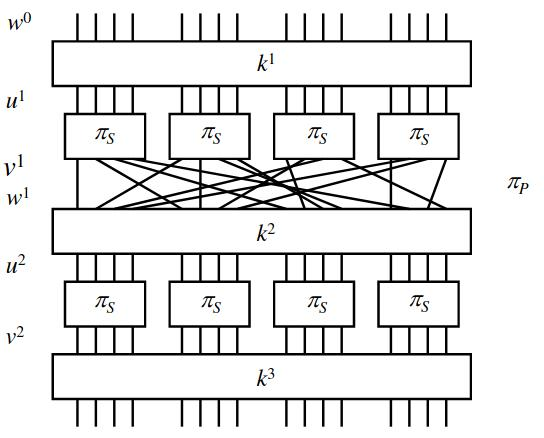
\includegraphics[scale = 0.45]{img/snp.jpg}
  \caption{Schema di una SNP. Fino al blocco $k^2$ escluso si ha il
    primo e unico round.}
  \label{fig:spn}
\end{figure}
\subsubsection{Struttura di Feistel}
Possiamo quindi parlare della \textbf{struttura di Feistel}.\\
Feistel cercava una cifratura ovviamente reversibile. Si usa un \textbf{decoder}
da $n$ a $2^n$ bit e poi un \textbf{encoder} da $2^n$ a $n$ bit, per cifrare il
testo in 
chiaro di $n$ bit. Tra il decoder e l'encoder si ha una 
struttura/permutazione che permette una sostituzione monoalfabetica di $2^n$
simboli, ovviamente questa non è fisicamente realizzabile con un circuito
elettronico.\\  
Si spezza quindi la permutazione in blocchi realizzabili in hardware che può
essere usato in serie o parallelo, con un'idea simile ad una SNP. Feistel per
approssimare la cifratura usa quindi piccoli moduli, alternando sostituzioni e
permutazioni come detto da Shannon.\\
Si prende quindi un testo in chiaro $m$, di $2\cdot w$ bit, e la chiave $k$, da
cui genero le $k^i$, con $i\in[1,n]$, chiavi derivate. Divido $m$ in $L_0$ e
$R_0$ che poi vengono trasformati in $L_iR_i$, con $i\in[1,n]$ (si noti la
natura del DES).\\
Si ha quindi la sostituzione, con $F$ round function come nel DES (o meglio
quella del DES è come questa):
\[L_i=L_{i-1}\oplus F(R_{i-1}, k^i)\]
per poi la permutazione:
\[L_i=R_{i-1}\]
\[R_i=L_{i-1}\oplus F(R_{i-1}, k^i)\]
Dopo tutti i round si cancella l'effetto dell'ultima permutazione che non
aggiunge sicurezza (in alternativa tale round può essere modificato). Si ottiene
infine $c$\\
La struttura di Feistel comporta che è più sicuro, ma più lento, all'aumentare
della grandezza di chiavi, blocchi, numero di round o all'aumentare della
complessità di $F$ o del sistema di generazione di chiavi derivate
etc$\ldots$.\\
La sfida non è solo la sicurezza ma anche l'efficienza. \\
Per decifrare con la struttura di Feistel applico al contrario le inverse delle
operazioni di cifratura. Il diagramma di una struttura di Feisel è simmetrico
(per questo annullo l'ultima operazione in fase di cifratura) tra cifratura  e
decifratura (al più dell'ordine dell'uso delle chiavi). Questa simmetria aiuta
lato hardware.
\subsubsection{Crittoanalisi Lineare}
La \textbf{crittoanalisi lineare} si basa sull'idea di approssimare la
trasformazione da $m$ a $c$ attraverso una funzione lineare. Si ha quindi
un'approssimazione parlando di base di funzioni non lineari. Si cercano
relazioni 
statistiche tra bit di $m$ e $u^j$, livello che precede le ultime applicazioni
di s-box. Si procede a ternativi con lo xor ottenendo combinazioni di bit
candidati per l'ultimo livello, vedendo se poi vale la relazione statistica. Si
cercano quindi di indovinare alcuni bit della chiave di partenza ``risalendo''
sulla SNP. Servono tanti tentativi, tante coppie $(c,m)$ etc$\ldots$.\\
Si applicano teoremi per eventi indipendenti a eventi dipendenti.\\
\textbf{Risentire questa parte (ultimi 10 minuti lezione 27 aprile)}.\\
Cambiare la chiave di cifratura spesso riduce le chance di questo attacco.\\
Possiamo quindi parlare della sicurezza del DES. \\
Coppersmith, nel 1994, studiando le s.box di DES disse: \textit{nessun
  bit di 
output di nessuna s-box dovrebbe essere troppo vicino all'output di una funzione
lineare. In particolare, se selezioniamo qualsiasi bit di uscita e qualsiasi
sottoinsieme dei sei bit di ingresso, la frazione di ingressi per cui questo bit
di uscita è uguale a xor di questi bit di ingresso non dovrebbe essere vicina a
0 o 1, ma piuttosto dovrebbe essere vicina a $\frac{1}{2}$}.\\
Si hanno anche tipi di attacchi che riguardano le implementazioni dei
crittosistemi e non la loro matematica. Sono detti \textbf{side channel attack}.
Si hanno anche i \textbf{timing attack} basati sul fatto che cifrare e decifrare
richiede tempo diverso per diversi input. Oppure attaccando sensori al circuito
per vedere quanta corrente serve per lavorare sui vari input. Nel 1999 si è
trovato con un timing attack il peso di Hamming sul DES. Ci sono stati timing
attack in grado di capire i vari pesi.\\ Si ha anche un attacco
di crittoanalisi lineare cercando di costruire buone approssimazioni per
ottenere infine l'ultima chiave. Studiando l'hardware crittografico durante il
funzionamento del sistema si possono inoltre aggiungere rumori etc$\ldots$,
magari anche scoprendo debolezze.\\
Bisogna quindi approfondire le s-box, la parte non lineare dei crittosistemi
visti. Per DES erano fatte a mano.\\
Ci sono in generale 3 modi, dal più vecchio che nuovo:
\begin{itemize}
  \item prendere s-box grandi e più grandi sono meglio è. Tali s-box vengono poi
  scelte a caso. Questa soluzione è molto grezza
  \item scegliere s-box a caso ma facendo test statistici tenendo le
  migliori. Soluzione migliore ma non ancora soddisfacente
  \item usare criteri matematici, come misure di non linearità, disuguaglianze
  per non linearità etc$\ldots$ Questi teoremi mitigano molti degli attacchi
  citati. AES usa questi criteri, con il discorso della \textit{wide trail
    strategy} 
\end{itemize}
Parlando dei \textbf{cifrari a flusso} si ha che vengono usati quando si hanno
tantissimi dati da cifrare, come ad esempio flussi video. La decifratura deve
avvenire su device mainstream poco potenti, come magari una TV.\\
La cifratura deve essere quindi ``leggera'' e si cifra ogni bit/byte facendo lo
xor con la chiave derivata, prodotta da un generatore di numeri casuali
,\textbf{Pseudo-Random Number Generator (\textit{PRNG})}). Il PRNG produce la
chiave derivata, di un bit/byte, che viene appunto poi usata in xor con il
plaintext.\\
I crittosistemi a flusso sono molto più performanti di quelli a blocchi e sono
più brevi da scrivere in codice ma come contro non si possono usare le stesse
chiave, in quanto la stessa chiave porta allo stesso messaggio cifrato,
indebolendo il sistema, creando relazioni tra testi in chiaro e cifrati. In
generale la sicurezza è data dalla qualità del PRNG. In generale:
\begin{itemize}
  \item la keystream deve avere un grande periodo, per rendere difficile la
  crittoanalisi. Per questo si riusano ``mix'' degli stati interni etc$\ldots$
  \item la keystream deve approssimare al meglio possibile una sequenza
  randomica, per non provare ad approssimare One Time Pad
  \item la chiave/seed del PRNG deve essere lunga almeno 128bit per evitare
  attacchi bruteforce
\end{itemize}
Il seed è condiviso da Alice e Bob, in quanto a parità di seed si ha
determinismo.\\  
Un cifrario a blocchi in modalità OFB si comporta come un cifrario a flusso.\\
\subsubsection{Linear Feedback Shift Registers}
Un tema importante sono i \textbf{registri a scorrimento}, \textbf{Linear
  Feedback Shift Registers (\textit{LFSR})}.\\
Sono stati creati per creare un keystream in modo più veloce di quello di un
cifrario a blocchi.\\
Bisogna generare un keystream $z_1,z_2,\ldots$, potenzialmente infinito ma non
periodico. Si parte da $n$ bit $k_i$. L'idea è quella di fare delle operazioni
xor con $k_1$ e $k_2$, da prendere a seconda di una certa maschera (se ho
associato 0 non lo considero se 1 si), per generare
gli altri $k_i$. Nel dettaglio:
\begin{itemize}
  \item è dato l'alfabeto $L=\{0,1\}$ ed è dato $c_0,\ldots
  c_{m-1}\in\mathbb{Z}_2$, con $m$ costante
  \item si parte con una sequenze $k_1,\ldots k_m$
  \item si pone $z_i=k_i,\,\,\,\forall i\in\{1,2,\ldots,m\}$ 
  \item $\forall i\geq 1$ si calcola $z_{i+m}$ usando la ricorrenza lineare di
  grado $m$, avendo che $z_{i+m}$ dipende dagli $m$ termini precedenti:
  \[z_{i+m}=\sum_{j=0}^{m-1}c_jZ_{i+j}\bmod\,\,2=\bigoplus_{j=0}^{m-1}(c_j\land
    z_{i+j})\] 
\end{itemize}
Si ha che scegliere $(k_1,\ldots,k_m)$ tutti uguali a 0 comporta la creazione di
sequenze di soli 0 quindi bisogna evitarlo.\\
Con $m=4$, ad esempio, posso produrre periodo 15, poco, e quindi il discorso del
periodo va approfondito, scegliendo $(c_0,\ldots,c_{m-1})$ in modo che ogni scelta
di $(k_1,\ldots,k_m)$ abbai periodo lungo.\\
\textbf{Esempio su slide}.\\
Si nota, dal punto di vista della sicurezza, l'uso di equazioni lineare per
generare il keystream con LFSR, che quindi vengono usati solo come parte di
tool più complessi. \\
Per la linearità si supponga che Eve conosca $2m$ chiavi derivate, $z_1,\ldots
z_{2m}$ e che conosca $m$. Può capire come sono state calcolate le chiavi della
seconda metà:
\[(z_{m+1},z_{m+2},\ldots, z_{2m})=(c_0,c_1,\ldots,c_{m-1})\cdot
  \left[
    \begin{matrix}
      z_1 & z_2 &\cdots &z_m\\
      z_2 & z_3 &\cdots &z_{m+1}\\
      \vdots & \vdots &\ddots &\vdots\\
      z_m & z_{m+1} &\cdots &z_{2m-1}
    \end{matrix}
  \right]
\]
e se la matrice fosse invertibile risalirei a $(c_0,c_1,\ldots,c_{m-1})$ e
purtroppo ``by design'', per costruzione, tale matrice è sempre invertibile. SI
fa quindi:
\[(c_0,c_1,\ldots,c_{m-1})=(z_{m+1},z_{m+2},\ldots, z_{2m})\cdot
  \left[
    \begin{matrix}
      z_1 & z_2 &\cdots &z_m\\
      z_2 & z_3 &\cdots &z_{m+1}\\
      \vdots & \vdots &\ddots &\vdots\\
      z_m & z_{m+1} &\cdots &z_{2m-1}
    \end{matrix}
  \right]^{-1}
\]
\subsubsection{RC4}
\textbf{RC4} è il cifrario a flusso più sicuro pensato. Creato nel 1987, uno dei
primi, dalla RSA. All'inizio però tale cifrario è stato mantenuto segreto. È
stato pubblicato in modo anonimo nel 1994 tramite \textit{reverse
  engineering}.\\
RC4 è usato in \textbf{SSL/TSL} (\textit{Secure Sockets Layer / Transport Layer
  Security}), usati nello standard della comunicazione web. È stato usato anche
in \textbf{WEP} (\textit{Wired Equivalent Privacy}), usato nello standard 802.11
(\textit{wireless LANs}).\\
Come funzionamento si ha la cifratura di un byte alla volta tramite permutazioni
casuali, ottenendo un periodo di keystream di $10^{100}$. Mediamente richiede
8-16 operazioni macchina per produrre ogni byte di $c$.\\
Si usa uno stato $S$ di 256 byte, che, in ogni momento, contiene le
permutazioni. Si usa una chiave $k$, lunga da 1 a 256 bytes, per inizializzare
$S$. Tale chiave non viene poi più usata.\\
Vediamo l'inizializzazione:
\begin{itemize}
  \item si mettono in $S$ i numeri da 0 a 255
  \item si crea un vettore temporaneo $T$ con i numeri da 0 a 255
  \item si ripete $k$ in $T$ tutte le volte necessarie a riempire $T$ (una sola
  se $k$ è di 256 bytes). Quindi si ha:
  \begin{algorithmic}
    \For {$i=0$ \textbf{to} $255$}
    \State $S[i]\gets i$
    \State $T[i]\gets k[i\bmod keylength]$
    \EndFor
  \end{algorithmic}
  \item si scambia ogni posizione di $S$ con una posizione determinata da $T$,
  tramite una funzione \texttt{swap}. Si ha quindi:
  \begin{algorithmic}
    \State $j\gets 0$
    \For {$i=0$ \textbf{to} $255$}
    \State $j\gets (j+S[i]+T[i])\bmod\,\,256$
    \State $swap(S[i],S[j])$
    \EndFor
  \end{algorithmic}
\end{itemize}
L'inizializzazione sono quindi due piccoli cicli for.\\
Una volta generato $S$ si passa a generare il keystream:
\begin{itemize}
  \item si parte da $S[0]$ per arrivare a $S[255]$. Una volta finito si riparte
  da capo (cosa ottenuta tramite il modulo)
  \item ad ogni iterazione l'elemento $S[i]$ è scambiato, tramite una funzione
  \texttt{swap}, con un altro $S[j]$, con $j$ che dipende dallo stato
  corrente. Questo aggiunge pseudocasualità
  \item si sommano, modulo 256, $S[i]$ e $S[j]$ per ottenere la posizione $t$,
  facendo quindi accesso indiretto,
  dell'elemento $z$ generato, con $z$ byte di chiave derivata
\end{itemize}
Anche per la generazione del keystream si ha quindi un codice piccolo, avendo un
ciclo infinito che dura fino a che serve cifrare i bytes.  
\newpage
Per il keystream si ha quindi:
\begin{algorithm}[H]
  \begin{algorithmic}
    \State $i\gets 0$
    \State $j\gets 0$
    \While {$\top$}
    \State $i\gets (i+1)\bmod\,\,256$
    \State $j\gets (j+S[i])\bmod\,\,256$
    \State $swap(S[i],S[j])$
    \State $t\gets (S[i]+S[j])\bmod\,\,256$
    \State $z=S[t]$
    \EndWhile
  \end{algorithmic}
  \caption{Calcolo keystream con RC4}
\end{algorithm}
La cifratura e la decifratura sono semplici:
\[c_i=m_i\oplus z\]
\[m_i=c_i\oplus z\]
Nonostante questo non si conoscono ancora attacchi efficaci data una chiave
lunga abbastanza, almeno 128 bit.\\
L'attacco fatto a WEP nel 2001 dipendeva da come era stato implementato RC4 in
WEP e non dall'algoritmo in sé.
\subsection{Sicurezza di Shannon}
Si è usato spesso lo xor bit a bit che garantisce sicurezza ma Shannon si è
chiesto se il calcolo della chiave fosse questione di pura potenza di calcolo.
Shannon si chiede se esistono crittosistemi sicuri \textbf{incondizionatamente},
ovvero a priori rispetto all'hardware disponibile dall'attaccante. Vediamo
quindi l'analisi di Shannon.\\
Si parte dal solito schema con Alice che comunica con Bob, tramite un canale, e
con Eve che ``ascolta''. Formalmente si ha:
\begin{itemize}
  \item $X$ una variabile casuale con valori nell'insieme dei plaintext $PT$
  \item $Y$ una variabile casuale con valori nell'insieme dei testi cifrati $CT$
  \item Alice sceglie, casualmente, $x\in PT$, la cifra e ottiene $y\in
  CT$. Tale $y$ viene spedito a Bob. Eve vede $y$ che per lei è totalmente
  casuale
  \item si assume che Alice sceglie $x$ in modo uniforme, per semplicità
  \item Eve conosce la distribuzione di probabilità su $X$, ovvero conosce
  $P(X=x)$ 
  \item se Eve legge $y$ può anche conoscere $P(X=x|Y=y)$ (aumenta la
  possibilità di avere alcuni testi in chiaro etc$\ldots$)
\end{itemize}
Shannon dice che il crittosistema è sicuro incondizionatamente se Eve,
osservando $y$, non impara nulla sulla distribuzione di probabilità dei testi in
chiaro, ovvero se:
\[P(X=x)=P(X=x|Y=y)\]
Ma questo implica che l'entropia di $X$ è uguale ell'equivocazione:
\[H(X)=X(X|Y)\]
Ma quindi la mutua informazione di sistema è:
\[I(X;Y)=0\]
e quindi $X$ e $Y$ sono \textbf{indipendenti} e Eve non ottiene alcuna
informazione da $y$. Eve vede solo rumore.\\
Ma per essere indipendenti significa che il canale è completamente rumoroso e
$y$ è scelto a caso senza partire da $x$ e quindi sembra assurdo parlando di
crittosistemi. \\
Shannon ha invece continuato lo studio e scopre che esiste un crittosistema
teorico completamente sicuro anche se con un'approssimazione pratica molto
efficace nota dal 1918, ovvero il \textbf{cifrario di Vernam}. La nuova versione
di tale cifrario viene chiamata \textbf{One Time Pad}, avendo che il
``taccuino'', traducendo Pad, contiene il keystream (e sia Alice che Bob devono
avere tale ``taccuino'' e questo è un problema). La chiave non va riutilizzata,
da qui one Time.\\
Alice cifra con la chiave del suo taccuino e Bob decifra di conseguenza,
entrambi distruggendo le pagine del taccuino con le chiavi usate.\\
La differenza tra One Time Pad e il cifrario di Vernam è che, in quest'ultimo,
non si usa una chiave usa e getta ma si può ripetere dopo un periodo molto
lungo. L'analisi quindi non è più impossibile ma molto difficile, è una buona
approssimazione. \\
In One Time Pad, si prende la chiave $k$ e si fa lo xor bit a bit. Il più sicuro
di tutti fa un'operazione lineare banale:
\[E_k(x)=x\oplus k\]
\[D_k(y)=y\oplus k\]
Il trucco è che la chiave $k$, lunga quanto il messaggio $m$, è davvero casuale
e non pseudocasuale (in Vernam 
ovviamente non è possibile la cosa ma la ripetizione dopo un lungo periodo è una
buona approssimazione). \\
Servono tanti bit casuali quanti la lunghezza del messaggio. La produzione di
tali bit, in due copie, una per Alice e una per Bob, è estremamente
dispendiosa.\\
Ovviamente prima Alice e Bob devono essersi accordati in modo sicuro sul
``taccuino'' e anche questo può essere complesso. 
\begin{teorema}
  Tale crittosistema è incondizionatamente sicuro.
\end{teorema}
\begin{proof}
  Si assumono PT e CT su alfabeti binari.\\
  Si ha la proprietà tale per cui:
  \[\forall x, \forall y\,\,\, \exists k \mbox{ unico t.c. } E_k(x)=y\]
  quindi dati $x$ e $y$ si ha una sola $k$ valida.
  Si ha anche la proprietà che:
  \[\forall y, \forall k\,\,\, \exists x \mbox{ t.c. } E_k(x)=y\]
  quindi sapendo solo $y$ posso solo sapere che tale messaggio cifrato può
  derivate da un qualunque $x$, scegliendo $k$ in modo appropriato.\\
  \textbf{Si ha quindi che è incondizionatamente sicuro non sapendo come
    scegliere}.\\ 
  Il tutto salta se la chiave è più corta. Si assume:
  \[|k|<|x|=|y|\]
  nel dettaglio:
  \[|k|=|x|-1=n-1\]
  Avendo $|k|<|x|$ dobbiamo usare nuovamente alcune bit di $k$.\\
  Quando Eve non ha ancora visto $c$ sa che Alice può scegliere qualunque $x$
  con probabilità $P(X=x)=\frac{1}{2^n}$, avendo che, osservato $y$, Eve si
  chiede i valori di $k$ usati per ottenere $x$ e vede che tali valori di $k$
  sono al più $2^{n-1}$. Quindi si ha:
  \[P(X=x|Y=y)=\frac{1}{2^{n-1}}\neq P(X=x)\]
  venendo meno la definizione di sicurezza incondizionata.
\end{proof}

In One Time Pad non si ha un seed di generazione quindi mentre in Vernam
serve.\\
One Time Pad è stato davvero usato tra Casa Bianca e Cremlino durante la Guerra
Fredda.\\
In ogni caso One Time Pad necessita di una quantità di chiavi molto grande, che
vanno scambiate prima in modo protetto. One Time Pad si usa solo con canali con
larghezza di banda molto bassa, quando la sicurezza e la privacy sono la prima
preoccupazione.
\subsection{Numeri Pseudocasuali}
Si è visto come molti algoritmi si basano su bit casuali. \\
Sorgenti casuali sono ``rare'' in natura e produrre hardware dedicato è
costoso.\\
Si usano quindi generatori pseudocasuali, i già citati PRNG, che partono da un
seed iniziale, causale e più piccolo possibile, per generare numeri che sembrano
casuali ad un osservatore esterno, che non sa nemmeno dire se una sequenza è
causale o pseudocasuale. Nessun algoritmo, eseguibile in tempo polinomiale sui
una TM deterministica, può capire se una sequenza è causale o pseudocasuale in
tempo polinomiale. Non si ha quindi una soluzione ``facile'' e la cosa non è in
dubbio. L'attaccante però potrebbe avere una \textbf{TM probabilistica}, che può
spesso risolvere problemi ``difficili'', semplificando la soluzione del
problema. \\
Dobbiamo quindi generare sequenze di bit pseudocasuali indistinguibili da quella
casuali avendo a disposizione una TM probabilistica.\\
Il seed lo si vuole il più corto possibile ma poi si genera una sequenza di bit
più lunga, parlando di ``allungare il seed'', anche se comunque si tratta solo
di una serie di conti a partire dal seed, unica fonte di casualità.
\begin{definizione}
  Definiamo il concetto di \textbf{indistinguibilità}, dal punto di vista
  computazionale, come il fatto che l'osservatore non ha abbastanza potenza
  computazionale per capire se la stringa in analisi sia casuale o meno. \\
  La perfezione si raggiungerebbe qualora il problema di distinguere o meno una
  sequenza causale fosse un problema intrattabile, non essendoci un algoritmo
  efficiente, ovvero polinomiale su una TM, dedicato.
\end{definizione}
La potenza computazionale dell'avversario comunque non è per forza limitata,
come detto, a macchine deterministiche ma potrebbe usare anche approcci
probabilistici.
\begin{definizione}
  Una \textbf{Probabilistic Turing Machine (PTM)} è una TM tale che,
  nell'applicazione della funzione di transizione tra stati, si hanno più stati
  possibili prossimi, come nelle NDTM, però la scelta cade solo su uno in modo
  casuale. Si ha quindi una sorta di secondo nastro con bit casuali,
  inizializzato all'inizio della computazione ogni volta in modo indipendente
  dalle precedenti computazioni, che mi dice quale stato successivo scegliere.
\end{definizione}
Per molti problemi non si sa se esiste un algoritmo deterministico polinomiale
ma potrebbe esserci un algoritmo probabilistico con probabilità d'errore minore
di $\frac{1}{2}$ e quindi basta fare più esecuzioni in parallelo (ma anche in
serie a seconda dell'hardware), esecuzioni che sono indipendenti tra loro per
il concetto di PTM. Ogni esecuzione a sua volta avrà probabilità d'errore minore
di $\frac{1}{2}$. La probabilità che tutte restituiscano una risposta sbagliata
si ottiene moltiplicando le varie probabilità, essendo tutte le esecuzioni
indipendenti, ottenendo che è minore di $\frac{1}{2^n}$, con $n$ numero di
esecuzioni. Possiamo dire che $\frac{1}{2^n}$ è una quantità davvero piccola
come probabilità, anche con $n$ non troppo grande (si ricordi la citazione per
cui $\frac{1}{2^{4096}}$ è stata definita come la probabilità che un tornado
ricostruisca un aereo distrutto in un campo e che 4096 computazioni non sono
così tante).\\
Si è discusso, nel tempo, del fatto anche un'azione naturale che sembra causale
lo è solo per i limiti dell'osservatore.\\
Nell'aspetto microscopico della natura, parlando di \textbf{meccanica
  quantistica}, dove la casualità gioca un ruolo essenziale, con una particella
che, nel momento in cui si trova nel mondo quantistico ha uno su infiniti stati
mentre nel mondo macroscopico uno su due. Si ha quindi che \textit{decade} negli
stati classici 0 e 1. Ogni volta che faccio un'osservazione si decade ad uno
stato classico e questo non è eliminabile, avendo che la \textbf{casualità}
esista effettivamente in natura.\\
Supponiamo quindi Eve abbia un PTM con, ovviamente, algoritmi probabilistici.
\begin{definizione}
  Un \textbf{PRNG} è un algoritmo, che può essere eseguito in tempo polinomiale
  su una TM deterministica, che calcola una funzione:
  \[G:\{0,1\}^k\to\{0,1\}^{l(k)},\,\,\,l(k)>k\]
  con $k$ numero di bit input.\\
  La funzione è tale che:
  \begin{itemize}
    \item per ogni algoritmo $D\in PPT$, dove $D$ sta per
    \textbf{distinguisher} e $PPT$ per \textbf{Polynomial Probabilistic Time},
    eseguito dall'attaccante. Tale algoritmo restituisce 
    0 se pensa che la sequenza non sia casuale, 1 altrimenti. Questi algoritmi
    possono essere eseguiti in tempo polinomiale su una PTM. Esistono in realtà
    classi di complessità per le PTM ma non si approfondiscono in questo
    contesto
    \item per tutti i polinomi $p(\cdot)$
    \item per tutti gli interi $k$ sufficientemente grandi. Si ragiona quindi in
    modo asintotico e più grande è $k$ meglio è
  \end{itemize}
  si ha, usando $\gets$ per dire ``preso a caso'' e chiamando:
  \begin{itemize}
    \item $\alpha=P[ x \gets \{0,1\}^k ; r \gets G(x) : D(r) = 1]$, avendo la
    probabilità, preso a caso $x$, sequenza di $k$ bit veramente causale, dato
    in pasto $x$ a $G$ che produce in output $l(k)$ bit assegnati a $r$, che a
    sua volta viene dato in pasto al \textbf{distinguisher} che restituisce 1,
    riconoscendo $r$ come sequenza casuale (sbagliando non essendo causale ma
    generata da $G$)
    \item $\beta=P[ r \gets \{0,1\}^{l(k)} ;  D(r) = 1]]$, avendo la probabilità
    che, preso a caso $r$, sequenza di $l(k)$ bit veramente causale, dato in
    pasto tale $r$ al \textbf{distinguisher} $D$ che, in tempo probabilistico
    polinomiale, restituisce 1, riconoscendo $r$ come sequenza casuale
    (azzeccando, essendo $r$ davvero casuale)
  \end{itemize}
  si ha:
  \[|\alpha-\beta|<\frac{1}{p(k)}\]
  quindi la distanza tra le distribuzioni di probabilità è minore di un
  $\frac{1}{p(k)}$, con $k$ però che cresce, avendo che $p(k)$ è in realtà una
  successione, con $p(\cdot)$ polinomio positivo che assume valori crescenti e
  quindi $\frac{1}{p(k)}$ decresce al crescere di $k$. Al crescere di $k$ la
  distanza tra le due probabilità va a 0 con velocità pari all'inverso del
  polinomio $p(k)$ (quindi non velocemente come con un esponenziale, fattore che
  porterebbe a dover ``chiedere troppo'' al PRNG, dovendo creare sequenze
  pseudocasuali davvero molto causali). Se il PRNG riesce a portare a poco
  quella differenza significa che abbiamo un buon algoritmo. Se le due
  probabilità sono distanti 0 si ha che il \textbf{distinguisher} non è in grado
  di capire se si ha a che fare con una sequenza casuale o meno, dando la stessa
  risposta sia sulla sequenza generata da $G$ che su quella davvero casuale.\\
  La distanza tra le due probabilità è quindi la ``capacità di barare'' di $G$,
  la capacità di ingannare qualunque \textbf{distinguisher} $D$.
\end{definizione}
\subsubsection{Linear Congruential Generator}
Vediamo quindi un esempio di PRNG, ovvero il \textbf{Linear Congruential
  Generator (\textit{LCG})}, usato per tanti anni ma ormai riconosciuto come non
 adatto all'uso in applicazioni etc$\ldots$ mentre non ha mai trovato,
 fortunatamente, spazio in crittografia. \\
Proposto nel 1951 da Lehmer è formato solo da equazioni lineari.
\begin{definizione}
  Definiamo formalmente il LCG.\\
  Presi accuratamente tre interi $a$, $b$ e $m$ tali che:
  \[0\leq a,\,\,\,\,b< m\]
  dato un seed intero $s$ tale che:
  \[0\leq s< m\]
  si ha il LCG definito come il sistema di equazioni:
  \[
    \begin{cases}
      x_0=s\\
      x_i=(ax_{i-1}+b)\bmod\,\,m,\,\,\,\,\forall i\geq 1
    \end{cases}
  \]
   La scelta di $a$, $b$ e $m$ è critica per trovare una sequenza non facile da
  predire. \\
  Questo generatore non allunga la sequenza di bit input ma non è il problema
  più grave. Il vero problema è che nella sequenza generata si hanno relazioni
  lineari e quindi se Eve trova quattro valori $x_0,x_1,x_2, x_3$, prodotti dal
  PRNG, può calcolare $a$, $b$ e $m$, risolvendo il seguente sistema:
  \[
    \begin{cases}
      x_1\equiv(ax_{0}+b)\bmod\,\,m\\
      x_2\equiv(ax_{1}+b)\bmod\,\,m\\
      x_3\equiv(ax_{2}+b)\bmod\,\,m
    \end{cases}
  \]
  Immaginando di plottare i valori di questo generatore come punti
  tridimensionali, si nota che si dispongono come piani, mostrando la linearità
  e quindi la conseguente debolezza. 
\end{definizione}
\subsubsection{Costruzione di un PRNG}
La definizione di PRNG non ci dice però come teoricamente dovrebbe essere un
buon generatore ma non ci dice come calcolarlo effettivamente. Si sono create
quindi varie batterie di test per testare i generatori di numeri casuali, anche
definiti dal NIST(National Institute of Standard and Technology) degli USA. Tra
i test si può vedere quanti zeri e uni ci sono nella sequenza di bit generata,
che devono essere circa uniformemente distribuiti. Un altro test è vedere 00,
01, 10 e 11 anch'essi dovrebbero essere circa uniformemente distribuiti e così
via aumentando le cifre. Un altro test è plottare tramite coordinate di punti e
vedere che si deve avere una distribuzione dei punti uniforme (e si hanno vari
test simili riempiendo un rettangolo o la superficie di una sfera). Si verifica
non ci siano pattern ripetuti. I vari test appena detti vengono anche fatti
prendendo, ad esempio, un bit ogni due etc$\ldots$. Si hanno potenzialmente
infiniti test (e quindi bisogna sceglierne una parte). \\
Il problema è quindi costruire una funzione $G$ tale che:
\[G:\{0,1\}^k\to\{0,1\}^{l(k)},\,\,\,l(k)>k\]
Tale funzione deve essere tale che allunga l'input, pur soddisfacendo i vincoli
dati in definizione.\\
Il primo problema pratico è capire quanto deve essere più lungo l'output. Un
secondo problema è capire se bisogna fare una funzione diversa per ogni valore
possibile di $l(k)$. In merito al secondo problema fortunatamente non dobbiamo,
in quanto, se si ha un PRNG $H$ che allunga di 1 e soddisfa tutti i vincoli
della definizione:
\[H:\{0,1\}^k\to\{0,1\}^{k+1}\]
possiamo costruire un altro $G$, del tipo:
\[G:\{0,1\}^k\to\{0,1\}^{l(k)},\,\,\,l(k)>k\]
La costruzione avviene in modo iterativo. Preso l'input $x_0$, di $k$ bit, lo si
allunga di quanto si vuole, dandolo in pasto a $G$. Avendo che anche $H$, che
allunga di 1, prende
in input una sequenza di $k$ bit (e quindi posso dargli in pasto $x_0$) si ha:
\begin{itemize}
  \item $x_1\sigma_1=H(x_0)$, avendo che $\sigma_1$ è un singolo bit
  \item $x_2\sigma_2=H(x_1)$, avendo che $\sigma_2$ è un singolo bit
  \item $\ldots$
  \item $x_{l(k)}\sigma_{l(k)}=H(x_{l(k)-1})$, avendo che $\sigma_{l(k)}$ è un
  singolo bit  
\end{itemize}
Avendo quindi:
\[x_i\in\{0,1\}^k\mbox{ e }\sigma_i\in\{0,1\},\,\,\,\forall i\in\{1,2,\ldots,
  l(k)\}\]
In output di $G$ si tiene quindi:
\[(\sigma_1,\sigma_2,\ldots, \sigma_{l(k)})\]
avendo quindi l'output allungato a $l(k)$ bit.\\
Questa costruzione è garantita formalmente e matematicamente da un teorema (che
non viene visto).\\
Ma dobbiamo capire come costruire $H$. Vediamo una costruzione interessante di
$H$, dove si usano le \textbf{funzioni one-way}, ovvero funzioni a ``senso
unico''. Una funzione one-way, che poi verranno meglio definite, in modo
informale è definibile come una funzione $f$ facile da calcolare ma
difficilissima da invertire, è un problema computazionalmente intrattabile,
essendo praticamente una \textit{permutazione}. Le
\textbf{funzioni di hash} sono one-way.\\
Quindi data $f$ one-way e $y$, che è detta \textit{impronta}, è difficile
calcolare $x$ tale che: 
\[f(x)=y\]
Un caso particolare di funzione one-way è una \textbf{funzione biunivoca}, che
presi $n$ bit in input restituiscono una sorta di permutazione di in output,
producendo un'altra sequenza di $n$ bit.\\
Se si ha che la funzione non è una permutazione, avendo magari dominio più
grande del codominio (come nelle funzioni hash) allora posso avere più $x$ che
produrrebbero $y$ tramite $f(x)$. Con una funzione one-way è difficile trovare
anche uno solo di questi $x$.\\
Un altro concetto necessario al calcolo di $H$ è quello di \textbf{hard-core
  bit}. \\
Se una funzione è difficile da invertire, essendo difficile calcolare $x$ tale
che $f(x)=y$, allora sarà difficile trovare i bit che compongono $x$. Magari non
sempre tutti i bit di $x$ sono difficili da trovare, per esempio il bit meno
significativo potrebbe essere facile da trovare. I bit difficili da calcolare,
che ovviamente non possono essere nessuno, sono detti appunto \textbf{hard-core
  bit}. \\
Si hanno quindi funzioni one-way e almeno alcuni bit dell'input che sono
hard-core. \\
Vediamo quanti possono essere tali hard-code bit. Non può essere di certo uno
solo, perché costruirei due input, con i due valori possibili di quel bit, e
calcolo la $f$ e vedo per quale dei due ottengo l'output giusto capendo quindi
quale valore assume quel bit (che non è quindi hard-core). Stesso discorso se si
suppone siano solo 2, avendo 4 possibili input.\\
Non posso quindi avere un numero \textbf{piccolo e costante} di bit hard-core.\\
Nemmeno un numero logaritmico sulla lunghezza dell'input andrebbe bene in
quanto si potrebbe usare il brute-force. Dato quindi $x\in\{0,1\}^n$ i bit
hard-core devono essere più di $\log_2n$, ad esempio $\frac{n}{4}$, altrimenti
possiamo prima calcolare il valore di tutti gli altri bit e poi provare tutte le
possibili combinazioni dell'hard-core fino a quando non troviamo la combinazione
corretta. Una quantità maggiore di $\log_2n$ significa una quantità lineare (o
funzioni particolari tra quelle logaritmiche e quelle lineari), come appunto
$\frac{n}{4}$, ma non più di 
lineare avendo che su $n$ bit posso al più avere $n$ hard-core bit. In pratica
si ha una certa frazione degli $n$ bit in input.\\
Bisogna introdurre un'altra definizione, quella di \textbf{predicato hard-core}.
\begin{definizione}
  Si definisce \textbf{predicato hard-core} un predicato $B$ che prende in input
  l'input della funzione e dice qual'è il valore di un hard-core bit.\\
  Il predicato è facile da calcolare in quanto conosce l'input.\\
  Quindi, data $f:\{0,1\}^n\to\{0,1\}^n$ funzione one-way (in particolare una
  permutazione one-way) che
  quindi prende $n$ bit in input e restituisce $n$ bit in output,il
  predicato $B$, calcolabile in tempo polinomiale da una TM deterministica, è: 
  \[B:\{0,1\}^n\to\{0,1\}\]
  che quindi prende $n$ bit in input e restituisce 1 bit.\\
  $B$ è un predicato hard-core per $f$ (un predicato) se:
  \[\forall \mbox{ algoritmo}\in PPT\land\forall\mbox{ polinomio }p(\cdot)
    \mbox{ si ha che }\exists n_{A,p} \mbox{ t.c}\]
  \[\forall n\geq n_{A,p},P[x\gets \{0,1\}^n ; b \gets A( f ( x)) : b = B(
    x)]\leq\frac{1}{2}+\frac{1}{p(n)}\] 
  Avendo quindi che per ogni algoritmo $A$ eseguibile dall'avversario su una PTM
  e per ogni polinomio $p$ esiste un numero $n_{A,p}$ (dipendente da $A$ e $p$)
  tale per cui per tutti gli $n$ maggiori di quella soglia, avendo quindi un
  discorso asintotico, vale che si ha una probabilità che è minore di
  $\frac{1}{2}$ sommata ad una quantità che tende a 0 velocemente quanto
  l'inverso di un qualunque polinomio passato (quindi non troppo
  velocemente). Nel dettaglio si parla della probabilità per cui, presa a caso
  una sequenza $x$ di $n$ bit, calcolata in modo facile computazionalmente
  $f(x)$, si assegna a $b$ il valore di tale calcolo di $f(x)$ dato in pasto
  all'algoritmo $A$ dell'avversario. La probabilità che $b$ sia davvero il
  risultato del predicato hard-core, ovvero $B(x)$, deve essere minore di
  $\frac{1}{2}+\frac{1}{p(n)}$. L'$\frac{1}{2}$ c'è in quanto si ha a che fare
  con un evento bernoulliano, avendo due risposte possibili, e quindi
  l'avversario deve azzeccare con probabilità che non supera $\frac{1}{2}$ per
  più di una quantità che tende a 0. In altri termini non può azzeccare con
  probabilità maggior di quella che avrebbe andando a caso, avendo solo due
  alternative. Quindi se $\frac{1}{p(n)}$ non tende a 0 significa che qualcosa
  si è capito in merito a come calcolare $b$. 
\end{definizione}
Avendo definito $f$ one-way e $B$ predicato hard-core, possiamo costruire il
PRNG $H$, con $H:\{0,1\}^k\to\{0,1\}^{k+1}$, in questo modo:
\[H(x)=f(x)||B(x)\]
avendo che $x$ e $f(x)$ sono di $k$ bit mentre $B(x)$ di un bit. La simbologia
$||$ indica la concatenazione e quindi $H(x)$ ha $k+1$ bit. Quindi aggiungo un
bit difficile da calcolare per l'attaccante ad una sequenza difficile da
invertire. L'output di $H$ è quindi difficile da predire (e la cosa è sostenuta
da un teorema che non vediamo).\\
Bisogna capire in pratica che $f$ funzione/permutazione one-way
scegliere (avendo poi che $B$ dipende da essa). Questa scelta è molto complessa
e per di più non è nemmeno mai stato 
dimostrato che esistano tali funzioni ma si hanno diverse candidate ma non si ha
ancora la dimostrazione matematica.\\
Vediamo quindi un caso speciale, una particolare costruzione, di Blum e
Micali.\\ 
Dato $g$ un generatore, fissato un numero primo $p$, di $\mathbb{Z}_p^*$, che è
sempre un \textbf{gruppo ciclico} (che quindi ha un generatore), e
$y=g^z\bmod\,p$ si ha che il bit più 
significativo dell'input $z$, ovvero $msb(z)$, è un predicato hard-core per la
\textbf{esponenziazione modulare} (è questo che hanno dimostrato Blum e Micali)
e quindi possiamo costruire un PRNG dalla 
esponenziazione modulare (che sarebbe nel dettaglio $y=g^z\bmod\,p$):
\[H(z)=g^z\bmod\,p||msb(z)\]
Si ha che $g^z\bmod\,p$ non solo è una funzione one-way ma anche una
permutazione one-way, permettendo di riottenere gli elementi di
$\mathbb{Z}_p^*$ in un ordine diverso, un ordine imprevedibile. È una tipica
permutazione usata in crittografia.\\
Ovviamente essendo $g$ un generatore di $\mathbb{Z}_p^*$ si ha che
$g\in\mathbb{Z}_p^*$.\\
Calcolare $g^z\bmod\,p$ può essere fatto in modo efficiente tramite
l'algoritmo \textbf{square and multiply} mentre calcolare $z$ partendo da $y$,
$g$ e $p$ è molto difficile, non avendo algoritmi polinomiali rispetto alla
dimensione dei valori in memoria, il numero di bit necessari per rappresentare
$\mathbb{Z}_p^*$, che è il più \textbf{grosso gruppo moltiplicativo} contenuto
in $\mathbb{Z}_p$. Si ricorda che gli elementi in $\mathbb{Z}_p^*$ possono 
assumere valore tra 1 e $p-1$, non 0, che non ha un inverso essendo un gruppo
moltiplicativo. Possiamo quindi dire che la dimensione dei valori in memoria è
$\log_2 p$, ovvero il numero di bit necessari a rappresentare $p$. Riuscire a
calcolare $z$ partendo da $y$, $g$ e $p$ è molto difficile e tale problema è
detto \textbf{problema del logaritmo discreto}, avendo che calcolare $z$
corrisponde a calcolare $\log_g y$ in un campo finito (da qui discreto). Non si
hanno neanche algoritmi probabilistici per il problema del logaritmo discreto ma
non si ha alcuna dimostrazione che non esista un algoritmo polinomiale. In base
a questa assunzione di complessità sul calcolo del logaritmo discreto si tratta
l'esponenziazione modulare come una funzione one-way.\\ 
Si conoscono pochissime altre funzioni candidate one-way, ancora meno che siano
permutazioni one-way, dovendo poi dimostrare che un certo bit sia hard-core bit
per tale funzione/permutazione.\\
Si ha però un teorema che viene in aiuto in questa situazione, un metodo
generale per calcolare, in modo semplice anche se la dimostrazione è molto
complessa, degli predicati hard-core associati a permutazioni one-way.\\ 
Serve prima una definizione
\begin{definizione}
  Prese due sequenze di $n$ bit $x=(x_1,\ldots,x_n)$ e $y=(y_1,\ldots,y_n)$ si
  ha che il prodotto interno modulo 2 tra le sequenze, $\langle x,y\rangle$, è
  definito tramite: 
  \[\langle x,y\rangle=^{def}\sum_{i=1}^n
    x_iy_i\bmod\,2=\bigoplus_{i=1}^n(x_i\land y_i)\]
  Era stato già visto coi \emph{registri a scorrimento}.
\end{definizione}
\begin{teorema}[Teorema di Goldreich–Levin]
  Data $f(x)$ una permutazione one-way sull'input $x$ possiamo estendere la
  permutazione ad una funzione $g$ di due argomenti, $x$ e $y$, concatenando $y$
  al valore di $f(x)$: 
  \[g(x,y)=f(x)||y\]
  avendo $|x|=|y|=n$.\\
  Una volta fatto questo si ha che la funzione, che è un predicato, $B(x,y)$
  definita: 
  \[B(x,y)=^{def}\langle x,y\rangle\]
  è, sempre, un predicato hard-core della funzione $g$, estensione di una
  qualunque permutazione one-way $f$. Si noti che $g$ ottenuta come appena detto
  è a sua volta una permutazione one-way.
\end{teorema}
\textit{Interessante che Levin sia lo stesso che, in contemporanea a Cook e in
  modo indipendente, scoprì la NP-completezza}. \\
Partendo quindi da una qualsiasi permutazione one-way $f$ ho perlomeno risolto
il problema di trovare il predicato hard-core.\\
Quindi, per il teorema di Goldreich–Levin, avendo a disposizione una
permutazione one-way su $\{0,1\}^n$ posso costruire il PRNG, che allunga di 1 il
numero di bit in ingresso:
\[H:\{0,1\}^{2n}\to \{0,1\}^{2n+1}\]
avendo:
\[H(x,y)=g(x,y)||B(x,y)=f(x)||y||\langle x,y\rangle\]
L'unico svantaggio è che il numero di bit di ingresso deve essere pari ma tutte
le funzioni booleane usate in crittografia hanno un numero pari di bit. Questo
problema è quindi trascurabile. Usando poi la costruzione iterativa vista
precedentemente posso costruire un PRNG $G$, con output lungo quanto voglio,
partendo da $H$.
\subsubsection{Dimostrazione di un PRNG}
Questa costruzione è dimostrata funzionare ed è sorretta da teoremi che non
vedremo. \\
Supponiamo ora di avere un algoritmo $G$ che si sospetta essere un PRNG e
vogliamo dimostrare che lo sia effettivamente. \\
Possiamo sottoporre il test ad una batteria infinita di test ma ovviamente non
possono essere infiniti in quanto non potrei dimostrare che li supera
tutti. Anche in questo caso si ha un teorema che ci salva, ad opera, nel 1985,
di Andrew Chi-Chih Yao, che anche lui, come spesso per chi studia problemi di
crittografia, arriva dal mondo dello studio della complessità
computazionale. Yao ha provato l'esistenza di un \textbf{test universale}, che
libera dall'onere di calcolare le infinite relazioni statistiche in infiniti
test.\\
Partiamo con una definizione.
\begin{definizione}
  Dato $G:\{0,1\}^k\to\{0,1\}^{l(k)}$ si ha che $G$ è \textbf{impredicibile}
  sse, $\forall i\in\{1,2,\ldots,l(k)\}$, $\forall p(\cdot)$ polinomio e
  $\forall A\in PPT$ algoritmo, dell'avversario, probabilistico eseguito su una
  PTM, $\exists 
  k_{A,p}$ tale che, $\forall k\geq k_{A,p}$ (avendo quindi una definizione
  asintotica): 
  {\small{\[P[x\gets\{0,1\}^k;(\sigma_1,\ldots,\sigma_{l(k)})=
        G(x);\hat{\sigma}_i\gets
        A(\sigma_1,\ldots,\sigma_{i-1}):\sigma_i=\hat{\sigma}_i]\leq   
        \frac{1}{2}+\frac{1}{p(k)}\]}}
  Quindi si estrae una sequenza casuale $x$ di $k$ bit che viene data in input a
  $G$, candidato generatore che allunga a $l(k)$. Per ogni bit diamo in input
  all'avversario i primi $i-1$ bit prodotti e si studia se $A$ è in grado di
  individuare il bit successivo. La probabilità di azzeccare tale bit, se si ha
  che $G$ è valido come PRNG, non deve essere significamene più grande di
  $\frac{1}{2}$, ovvero della scelta causale avendo 2 scelte per il bit, o 0 o
  1. La probabilità deve essere quindi minore uguale di $\frac{1}{2}$ più una
  quantità che tende a 0 al crescere di $k$, anche se non troppo velocemente,
  tendendo a 0 come l'inverso di un polinomio qualunque. Tutto questo deve
  valere per ogni algoritmo $A$ dell'attaccante.\\
  Informalmente $G$ è impredicibile sse il problema di ``indovinare'' l'i-esimo
  bit della sequenza dati i primi $i-1$ bit è un problema computazionalmente
  intrattabile, dove ``indovinare'' significa ``indovinare significativamente
  meglio rispetto al semplice lancio di una moneta''.
\end{definizione}
\begin{teorema}[Teorema di Yao]
  L'algoritmo $G$ è un PRNG sse $G$ è impredicibile.\\
  In letteratura questo test universale è anche detto \textbf{next bit test}.
\end{teorema}
\subsubsection{Cifratura Ciclica}
Finora però è stata vista la teoria, passiamo a vedere come si genera realmente
una sequenza casuale di bit.\\
Nel 1982 Meyer e Matyas proposero uno schema che si basa sull'uso di un
crittosistema simmetrico, in cui si fissa una \textbf{master key} che è il seme
casuale, e si usa il testo in chiaro come ``contatore''. Si cifra ciclicamente
ogni elemento con la chiave e si generano ogni volta nuovi bit, in una sequenza
imprevedibile che supera il next bit test. In pratica, come visualizzabile in
figura \ref{fig:prng}:
\begin{itemize}
  \item si parte dal seed/master key che produce una sequenza di chiavi derivate
  \item si usa un contatore con periodo $\bmod n$
  \item il valore del contatore è usato o come chiave o come plaintext in un
  crittosistema simmetrico 
  \item ogni volta che si usa il crittosistema simmetrico si incrementa il
  contatore
\end{itemize}
\textit{Per rafforzare ulteriormente questo schema possiamo usare una sequenza
  di input più complicata}. 
\begin{figure}
  \centering
  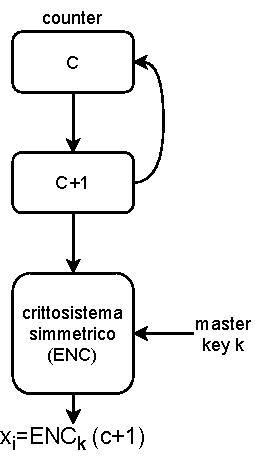
\includegraphics[scale = 0.8]{img/prng.pdf}
  \caption{Schema di Meyer e Matyas}
  \label{fig:prng}
\end{figure}
Anche la modalità operativa OFB di un crittosistema simmetrico può essere usata
per generare un keystream che è considerabile come l'output di un algoritmo
PRNG.\\
\subsubsection{ANSI X9.17}
Vediamo ora uno dei più conosciuti PRNG conosciuti in crittografia, ovvero
\textbf{ANSI X9.17}, che è appunto diventato standard e piene usato in PGP.\\
ANSI X9.17 usa 3DES ma è generalizzabile ad altro crittosistemi.\\
In input si hanno 2 elementi:
\begin{itemize}
  \item $DT_i$, una rappresentazione a 64bit della data e dell'ora correnti. È
  aggiornato in ogni blocco pseudocasuale generato 
  \item $V_i$, un seed a 64bit
\end{itemize}
Come chiavi si hanno $K_1$ e $K_2$, entrambe di 64bit, anche se DES usa solo
56bit (scartando i bit di parità). Le chiavi sono usate nei 
tre moduli con 3DES, usato in modalità EDE (nell'ordine usando $K_1$, $K_2$,
$K_1$): 
\[encryption – decryption – encryption\]
\newpage
Si hanno quindi due output:
\begin{itemize}
  \item $R_i$, che è un blocco causale di 64bit
  \item $V_{i+1}$ che è il valore aggiornato del seed
\end{itemize}
Si ha uno schema del tipo:
\begin{figure}[H]
  \centering
  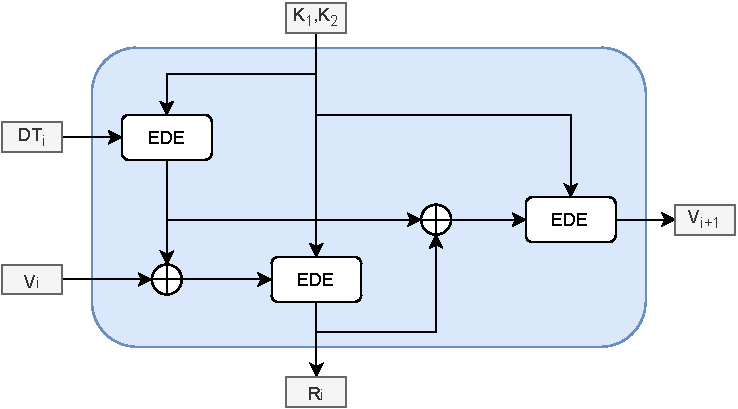
\includegraphics[scale = 0.9]{img/ansi.pdf}
\end{figure}
Si nota che:
\[R_i=EDE_{K_1,K_2}(V_i\oplus EDE_{K_1,K_2}(DT_i))\]
\[V_{i+1}=EDE_{K_1,K_2}(R_i\oplus EDE_{K_1,K_2}(DT_i))\]
Usando 3DES si può quindi che si usa una chiave di 112bit e che che si usano in
totale 9 DES per cifrare e decifrare, con $DT_i$ e $V_i$ che cambiano dopo la
produzione di ogni singolo valore di output. Usando 9 DES, quindi 9 cifrature,
non si hanno performance particolarmente elevate, un generatore di qualità
inferiore potrebbe essere più ufficiente. Usando 9 DES ANSI X9.17 è praticamente
inviolabile, serve una quantità incredibile di informazioni per comprometterlo,
anche perché la crittoanalisi sul singolo DES è comunque difficile, e
anche se Eve venisse a sapere $R_i$ non riesce a capire il valore successivo. 
\subsubsection{BBS Generator}
\textbf{Questo generatore viene giusto accennato a lezione}.\\
Nel 1986 è stato poi proposto il \textbf{Blum, Blum and Shub (\textit{BBS})
  generator}, dai nomi dei tre crittografi che lo hanno studiato. \\
Questo generatore sfrutta i numeri primi.\\
Si prendano $p$ e $q$, primi e grandi tali che:
\[p\equiv q\equiv 3\bmod\, 4\]
quindi facendo il resto della divisione di entrambi i numeri primi per 4 viene
3.\\ 
Sia $n=p\cdot q$ e $s$ casuale tale che $GCD(s,n)=1$, quindi invertibile modulo
$n$. Si ha quindi che $s$ non è multiplo di $p$ o $q$.\\
Si genera quindi una sequenza di bit $B_1,B_2,\ldots$ secondo il seguente
algoritmo:
\begin{algorithm}
  \begin{algorithmic}
    \Function{BBS}{$s,p,q$}
    \State $n\gets p\cdot q$
    \State $X_0\gets s^2\bmod\,n$
    \State $i\gets 1$
    \While {$\top$}
    \State $X_i\gets X_{i-1}^2\bmod \,n$
    \State $B_i=X_i\bmod\,2$
    \EndWhile
    \EndFunction
  \end{algorithmic}
  \caption{Algoritmo del Blum, Blum and Shub generator}
\end{algorithm}
Avendo che $B_i=X_i\bmod\,2$ equivale a $B_i\gets lsb(X_i)$.\\
Si noti che $X_0$ è un valore in $\mathbb{Z}_n$, compreso tra 2 e $n-1$.\\
La sicurezza si basa sulla difficoltà di fattorizzazione, anch'essa comunque non
ancora dimostrata e si può provare che BBS supera il next bit test, non
esistendo un algoritmo polinomiale che dati i primi $k$ bit della sequenza di
output, $B_i,\ldots,B_k$ sia in grado di indovinare il $k+1$ bit, $B_{k+1}$, con
probabilità significativamente maggiore di $\frac{1}{2}$.
\section{Crittosistemi a Chiave Pubblica}
Vediamo ora i \textbf{crittosistemi a chiave pubblica (\textit{Public-Key
    Cryptsystems})}.\\
Questi crittosistemi nascono nel 1975 da un problema dei crittosistemi
simmetrici: Alice e Bob devono conoscere la stessa chiave segreta $k$. \\
La svolta nel 1975 è che l'agreement della chiave viene fatto su un canale
pubblico, con paper pubblicato nel 1976.\\
Nel 1977 nasce RSA, dalle menti di Ronald Rivest, Adi Shamir e Leonard
Adleman, il crittosistema a chiave pubblica più famoso e usato, con 
paper pubblicato nel 1978.\\
Il problema finora riscontrato, con Alice e Bob che devono conoscere la stessa
chiave segreta $k$, si materializza qualora non sia possibile usare un canale
sicuro per scambiarsi la chiave, cosa abbastanza comune. \\
Per tutta la seconda metà degli anni sessanta si è studiata la complessità
computazionale, studiando quanto sono complicate le operazioni che vengono
svolte algoritmicamente, nascendo concetti come NP-completezza etc$\ldots$,
raccolti nel 1978 nel famoso testo di Garey e Johnson. Si studia quindi come
alcune operazioni siano facili se si conosce una certa informazione segreta e
difficili altrimenti (le funzioni one-way diventano facili da invertire se si
conosce tale informazione). Ma resta il problema di Alice e Bob che devono
scambiarsi tale informazione segreta, cosa che viene fatta su un canale pubblico
dove Eve ascolta.\\
Si trova anche un modo per gestire efficientemente le chiavi, nel caso in cui
Alice debba comunicare con più persone.\\
L'idea dietro la crittografia a chiave pubblica, idea del 1976/1977 di Diffie e
Hellman, è usare algoritmi diversi per 
cifrare e decifrare, con quello per decifrare che resta segreto mentre quello
per cifrare resta pubblico, si rende pubblica la chiave di
cifratura. L'attaccante è quindi in una posizione di vantaggio rispetto ai
crittosistemi simmetrici, tutti possono cifrare il messaggio ma solo il
destinatario può decifrarlo. \\
Per capire meglio l'idea (e i problemi) vediamo un'analogia. Si supponga che
Alice voglia mandare un messaggio a Bob. Tale messaggio viene mandato
fisicamente, tramite una scatola chiusa a chiave. Alice dice a Bob che le deve
mandare il messaggio e Bob manda la cassetta di sicurezza, con il lucchetto
aperto di cui solo lui ha la chiave. Alice scrive il messaggio, lo mette nella
cassetta e chiude il lucchetto, che ora solo Bob può riaprire, e lo rispedisce a
Bob. Il problema è che Eve può intercettare la scatola aperta e sostituirla,
impersonificando sia Alice che Bob a seconda del punto di vista. Eve potrebbe
fare quello che vuole con la scatola sostituita, sostituendo il messaggio per
Bob. Questo è un problema non risolto. \\
Alice non può essere sicura che il lucchetto quindi sia di Bob e quindi usa
anche un suo lucchetto (e non quello di Bob) ma a questo punto sia Eve che Bob
non possono più aprire. Bob quindi chiude anche il suo lucchetto e la rimanda ad
Alice che toglie il suo e lo rimanda a Bob, che toglie il suo e legge il
messaggio. Quindi sembra che basti mandare più volte il messaggio per risolvere
il problema, complicando il protocollo di trasmissione, ma Eve può comunque
inserirsi, rimandando a Alice la scatola con entrambi i lucchetti (col secondo
suo e non di Bob), facendo una cosa simile anche con Bob per non destare
sospetti. Se Bob ha sospetti deve comunicarlo ad Alice. Eve sta facendo
l'attacco \textbf{man in the middle}. \\ 
Formalizziamo quindi meglio il problema.\\
Bob sceglie 2 algoritmi/chiavi (gli algoritmi dipendono unicamente dalla chiave
quindi posso usare i due termini in modo indistinto):
\begin{itemize}
  \item $E_B$ per cifrare
  \item $D_B$ per decifrare
\end{itemize}
tali che, ovviamente:
\[\forall m\in PT,\,\,D_B(E_B(m))=m\]
e devono essere tali per cui deve essere intrattabile ottenere $D_B$ da $E_B$.\\
Bob rende pubblico $E_B$ e tiene segreto $D_B$.\\
Se Alice vuole spedire $m$ a Bob calcola $E_N(m)$, l'algoritmo è pubblico, e lo
manda a Bob, che calcola $D_B(E_B(m))=m$. Se Eve intercetta $E_N(m)$ deve
risolvere un problema intrattabile per ottenere $B_B$. Il problema è che Alice,
se parte di una grande comunità di utenti, deve conoscere tutti gli algoritmi di
cifratura e questo è impraticabile, anche perché in caso di sospetti Bob
comunica la cosa ad Alice.\\
Per risolvere il problema sia Alice che Bob hanno i propri algoritmi
\begin{itemize}
  \item $E_A,E_B$ per cifrare
  \item $D_A,D_B$ per decifrare
\end{itemize}
tali che \textbf{commutino} gli algoritmi di cifratura e decifratura:
\[\forall m\in PT,\,\,E_A(E_B(m))=E_B(E_A(m))\]
\[\forall m\in PT,\,\,D_A(D_B(m))=D_B(D_A(m))\]
Ora non è necessario mettere pubblici i due $E$ ma bisogna tenere 
segreti i due $D$.\\
Alice infatti calcola $E_A(m)$ e lo manda a Bob che calcola $E_B(E_A(m))$ e
manda il risultato ad alice che calcola $D_A(E_B(E_A(m)))$ e rimanda il
risultato a Bob. Bob quindi calcola $D_B(D_A(E_B(E_A(m))))$ ma questo è uguale a
$D_A(D_B(E_B(E_A(m))))$ che equivale a $D_A(E_A(m))$ che equivale a $m$
($D_i(E_i(x))$ praticamente si semplificano).\\
Alice quindi usa solo $E_A$ e $D_A$ e in caso di sospetto gli basta cambiare
questa coppia.\\
Anche in questo caso Alice seleziona un elemento di una famiglia di coppie di
algoritmi di cifratura/decifratura, scegliendo una \textbf{chiave pubblica}
$k_{p_A}$ e la conseguente \textbf{chiave privata} $k_{s_A}$. Ovviamente si ha
che:
\begin{itemize}
  \item $\forall m\in PT,\,\,\,D_{k_{s_A}}(E_{k_{p_A}}(m))=m$
  \item è intrattabile ottenere $k_{s_A}$ da $k_{p_A}$
  \item in generale, l'uso previsto deve essere facile, mentre tutti gli usi
  imprevisti devono essere molto difficili  
\end{itemize}
Guardando le due versioni del protocollo viste sopra (la prima è quella con il
singolo invio e la seconda è quella con il doppio invio):
\begin{itemize}
  \item nella prima versione $k_{p_A}$ deve essere pubblica
  \item nella seconda versione $k_{p_A}$ può essere pubblica
\end{itemize}
In entrambe $k_{s_A}$ deve essere segreta.\\
Il canale che abbiamo descritto è criptato ma non autenticato. Bisogna capire,
quando Alice riceve la chiave pubblica di Bob, come può essere sicura di non
aver ricevuto invece la chiave di Eve.\\
Bisogna ora capire come implementare gli algoritmi di cifratura e decifratura,
le ``scatole segrete'' e
come generare le coppie di chiavi, quella pubblica e quella segreta.\\
Per la prima domanda si usano funzioni one-way, $f:\mathbb{N}\to\mathbb{N}$,
come già descritto precedentemente. Alice calcola praticamente $f(m)$ ma diventa
difficile anche per Bob, non solo per Eve. Si aggiunge quindi che le funzioni
one-way abbiamo una \textbf{trapdoor}, avendo che tali funzioni sono difficili
da invertire senza conoscere tale trapdoor e facili altrimenti. Bob quindi può
calcolare $x$ tale che $f(x)=y$. Tale informazione segreta deve essere
comunicata a Bob ma tale informazione viene rimescolata nella trasmissione.
\begin{definizione}
  Si ha che $f$, $f:\mathbb{N}\to\mathbb{N}$, è one-way se:
  \begin{itemize}
    \item $f$ può essere calcolata in tempo polinomiale da una macchina di
    Turing deterministica (cioè, è facile da calcolare)  
    \item esistono due polinomi, rispetto a $n$ numero di bit necessari a
    rappresentare l'input $x$, $p(\cdot)$ e $q(\cdot)$ tali che:
    \[p(|x|)\leq |f(x)|\leq q(|x|)\]
    avendo che l'output di $f$ non deve essere corto (il valore assoluto qui
    indica la lunghezza). 
    \item per ogni algoritmo $A$ dell'avversario, eseguito in tempo polinomiale
    su una PTM, e per ogni polinomio $p(\cdot)$ esiste un numero naturale
    $n_{A,p}$ si ha lo schema, detto \textbf{negligible trascurable} (\textit{lo
      sono anche tutti gli schemi simili già visti}):
    \[\forall n\geq n_{A,p}\,\,\,P[x\gets\{0,1\}^n; x'\gets A(f(x)):
      f(x)=f(x')]\leq \frac{1}{p(n)}\]
    Il calcolo è difficile per la $f$ non perché l'input è troppo corto, per
    quanto detto nel secondo punto
  \end{itemize}
\end{definizione}
Sin ricorda che queste funzioni one-way non si ha certezza che esistano, non si
riesce a dimostrare la loro esistenza. Se si avesse $P=NP$ sicuramente tali
funzioni non esisterebbero (perché si risolverebbe polinomialmente lo studio di
tutti i possibili alberi di computazione della NDTM per trovare
l'inversa). D'altro canto se si dimostrasse l'esistenza di anche 
solo una funzione one-way si avrebbe $P\neq NP$, questa è la
\textbf{contronominale} (e non l'inversa) dell'affermazione precedente. Da
questa affermazione si coglie il problema di capire se esiste una funzione
one-way. Si potrebbe comunque avere 
$P\neq NP$ senza avere che esista alcuna funzione one-way, avendo comunque che
invertire una funzione one-way deve essere ``quasi sempre''
difficile. Quest'ultima è l'\textbf{inversa} della prima affermazione.\\
In crittografia si lavora inoltre su permutazioni one-way su $\{0,1\}^n$.\\
\textbf{Dato che non si sa se $P\neq NP$ o $P=NP$ si assume che esista almeno
  una funzione one-way}.\\
Un esempio di probabile funzione one-way è l'\textbf{esponenziazione modulare},
solitamente modulo $p$, con $p$ numero primo. Si considera il campo
$\mathbb{Z}_p$ e il gruppo moltiplicativo, il più grosso contenuto in
$\mathbb{Z}_p$, $\mathbb{Z}^*_p=\{1,2,\ldots, p-1\}$.  Si ha che
$\mathbb{Z}^*_p$ è un gruppo ciclico:
\[\exists g\in \mathbb{Z}^*_p \mbox{ t.c. } \mathbb{Z}^*_p=\{g^0,g^1,\ldots
  g^{p-2}\}\]
(avendo che ho $p-1$ elementi ma l'esponente parte da 0 si ha che l'esponente
massimo è $p-2$). \textbf{Gli elementi calcolati tramite $g^i$ si ottengono in
  ordine permutato}, cosa che rende il problema intrattabile da invertire. Si ha
che $g$ genera i vari valori ciclicamente.\\ 
L'esponenziazione modulare è quindi una funzione:
\[f:mathbb{N}\to \mathbb{Z}^*_p\]
definito come:
\[f(z)=g^z\bmod\,\,p\]
\textbf{Ogni esponenziazione modulare produce una permutazione one-way degli
  elementi di $\mathbb{Z}^*_p$}.
\begin{esempio}
  Vediamo un esempio.
  Si ha che $\mathbb{Z}_5=\{0,1,2,3,4\}$ e quindi:
  \[\mathbb{Z}^*_5=\{1,2,3,4\}\]
  Si ha che $2$ è un generatore di $\mathbb{Z}^*_5$:
  \[\mathbb{Z}^*_5=\{2^0,2^1,2^2,2^3\}=\{1,2,4,3\}\]
  e quindi:
  \[f(z)=2^z\bmod\,\,5\]
  Nell'esempio si è usato $p=5$ mentre in crittografia solitamente $p$ è un
  numero primo rappresentabile da almeno 1024 bit, quindi non piccolo.
\end{esempio}
Data $x$ si calcola $g^x\bmod\,\,p$ in tempo polinomiale e si assume $0\leq
x\leq p-2$ (per la ``rotazione'' del modulo). Fare $\bmod\,\,p$ rende difficile
invertire. \\ 
La grandezza dell'input è il numero di bit necessari a rappresentare
$\mathbb{Z}^*_p$, quindi:
\[n=\log_2p\]
Potrei pensare di fare, avendo $x_{n-1},\ldots, x_1, x_0$ come la
rappresentazione binaria di $x$, rappresentazione del tipo:
\[x=\sum_{j=0}^{n-1}x_j2^j\]
Avrei una cosa del tipo:
\begin{algorithm}[H]
  \begin{algorithmic}
    \Function{ModExp}{$p,g,x$}
    \State $result\gets 1$
    \While {$x>0$}
    \State $result \gets result \cdot g\bmod\,\,p$
    \State $x\gets x-1$
    \EndWhile
    \State \textbf{return} $result$ 
    \EndFunction
  \end{algorithmic}
  \caption{Primo tentativo non efficiente di calcolo esponenziazione modulare}
\end{algorithm}
In pratica avrei che $result$ contiene:
\[g^0,g^2,\ldots,g^x\bmod\,\,p\]
Ma avrei un numero di iterazioni esponenziale rispetto a $n$, infatti si
avrebbe: 
\[x\cong 2^n\]
C'è però un modo per calcolarlo in tempo polinomiale, passando la
rappresentazione in binario di $x$. Posso fare quindi:
\[g^x=
  g^{\sum_{j=0}^{n-1}x_j2^j}=\prod_{j=0}^{n-1}x_j2^j=\prod_{j=0}^{n-1}
  (g^{2^j})^{x_j}\bmod \,\,p\] 
Basta quindi calcolare $g^{2^j}$ per i vari $j$, da 0 a -1, e moltiplicarli per
$x_j=1$ (solo quei conti per cui si ha $x_j=1$ influiscono sul risultato) e
questo si fa in tempo polinomiale. Questo algoritmo è detto
\textbf{square-and-multiply}. Ragiono quindi tramite una maschera di bit
prendendo solo i valori in corrispondenza di 1.\\
Conviene inoltre salvarsi i $g^{2^j}$. Vediamo lo pseudocodice:
\begin{algorithm}[H]
  \begin{algorithmic}
    \Function{ModExp}{$p,g,x$}
    \State $result\gets 1$
    \For {$j=n-1$ \textbf{to} $0$}
    \State $result \gets (result \cdot result)\bmod\,\,p$
    \If{$x_j==1$}
    \State $result \gets (result \cdot g)\bmod\,\,p$
    \EndIf
    \EndFor
    \State \textbf{return} $result$ 
    \EndFunction
  \end{algorithmic}
  \caption{Algoritmo square-and-multiply per esponenziazione modulare}
\end{algorithm}
\textbf{Esempio su slide}.\\
L'operazione inversa è detta \textbf{logaritmo discreto} e non si è ancora
dimostrato essere facile. Sono dati, per questo problema, un numero primo $p$,
un generatore $g$ per $\mathbb{Z}_p^*$ e $y\in\mathbb{Z}_p^*$. Si calcola
$x\in\{0,1,\ldots,p-2\}$ tale che $g^x\equiv y\bmod\,\,p$. Tale calcolo è in
tempo esponenziale sul numero di bit input, avendo $n=\log_2p$. Elencare tutti
gli elementi di $\mathbb{Z}_p^*$ richiede quindi tempo $O(p)=O(2^n)$.\\
Si usa quindi l'esponenziazione modulare per nascondere il messaggio ma serve
una trapdoor per permettere a Bob di estrarre il messaggio.\\
Vediamo ora un'altra funzione one-way, il \textbf{prodotto tra due numeri
  primi}, $n=p\cdot q$, con $p$ e $q$ primi. Ogni numero naturale ammette
un'unica scomposizione in fattori primi, 
a meno dell'ordine degli stessi. Il prodotto ovviamente è in tempo polinomiale.
L'inverso del prodotto $n=p\cdot q$, con $p$ e
$q$ primi è detto \textbf{fattorizzazione}, che, dato $n$, consiste quindi nel
capire $p$ e $q$. I numeri sono espressi in binario. La dimensione dell'input di
questo problema è il numero di bit necessari a rappresentare $n$, $p$ e
$q$. Diciamo inoltre che si ha un numero $m$ tale che $m=\log_2n$. Diverse
istanze del problema sono abbastanza difficili, con numeri grandi, almeno 2048
bit, e che siano appunto prodotto di esattamente due numeri primi, che possono
essere scelti anche in modo accurato per avere la sicurezza migliore. Tali primi
devono essere circa della stessa dimensione, 1024 bit ciascuno, ma con valori
abbastanza diversi per non avere il risultato vicino a $\sqrt{n}$. \\
Non esiste un algoritmo polinomiale su $n$, per fattorizzare, neanche
probabilistico. Il numero di bit di $n$ è al più la somma dei bit necessari per
i due numeri primi.\\
\textbf{Esempio di RSA-768 su slide}.\\
L'algoritmo naive prevede la divisione di $N$ per tutti gli interi da 2 a
$\sqrt{n}$ in tempo:
\[O(\sqrt{n})=O(\sqrt{2^m})=O(2^{\frac{m}{2}})\]
quindi esponenziale, anche se ovviamente basta trovare o $p$ o $q$.\\
\subsection{Protocollo Diffie-Hellman}
Diffie ed Hellman nel 1976 pubblicano un paper su un protocollo molto semplice
che sua solo canali pubblici.\\
Alice e Bob scelgono insieme una chiave segreta, avendo quindi un \textbf{key
  agreement protocol}. Scelgono sul canale pubblico un primo $q$, lavorando su
$\mathbb{Z}_q^*$. Ovviamente lo sa anche Eve essendo un canale pubblico. Alice e
Bob scelgono anche il generatore $g$, che sa anche Eve. Alice sceglie a caso
$x_A$, $0<x_A<q-1$ e lo tiene segreto (non 0 perché Eve lo sgamerebbe
subito). Anche Bob sceglie a caso $x_A$, $0<x_B<q-1$ e lo tiene segreto (non 0
perché Eve lo sgamerebbe subito). Si procede così:
\begin{itemize}
  \item Alice calcola $g^{x_A}\bmod\,\,q$ e lo manda a Bob, ma anche ad Eve
  \item Bob calcola $g^{x_B}\bmod\,\,q$ e lo manda a Alice, ma anche ad Eve
  \item Alice calcola $(g^{x_B})^{x_A}=g^{x_A\cdot x_B}=k$, che Eve vede
  \item Bob calcola $(g^{x_A})^{x_B}=g^{x_A\cdot x_B}=k$, che Eve vede
  \item $k$ è la chiave segreta
\end{itemize}
Eve conosce quindi $q$, $g$, $g^{x_A}$ e $g^{x_B}$.\\
Eve non può conoscere $k$ e per ottenere $x_A$ e $x_B$ da $k$ dovrebbe calcolare
un logaritmo discreto.\\
Eve potrebbe calcolare $g^{x_A\cdot x_B}$ partendo da $g^{x_A}$ e $g^{x_B}$ che
conosce ma questo sembra anche lui un problema intrattabile, detto
\textbf{problema di Diffie-Hellman}.\\
\textbf{Esempio su slide}.
\subsection{Crittosistema di El Gamal}
El Gamal, nel 1984, propose un crittosistema che si basa sulla difficoltà di
calcolare $k_s$ da $k_p$ e di ottenere $m$ da $c=E_{k_p}(m)$ per il problema del
logaritmo discreto.\\
El Gamal sfruttò questo per porre le basi al sistema delle firme digitali. \\
Anche qui bisogna vedere come calcolare in primis la coppia di chiavi.
Si procede così:
\begin{itemize}
  \item si sceglie un primo a caso $q$, lavorando su $\mathbb{Z}_q^*$
  \item si sceglie il generatore $g$
  \item si sceglie un intero $a$, $0<a<q-1$, e si calcola $g^a\bmod\,\,p$. Si ha
  che $a$ è la chiave segreta $k_s=a$
  \item la chiave pubblica è la tripla $k_p=(q,g,g^a)$
\end{itemize}
Eve per ottenere $k_s$ da $k_p$ dovrebbe calcolare $\log_g g^a$, ma è
difficile.\\
Per cifrare si ha:
\begin{itemize}
  \item Alice manda $m\in\mathbb{Z}_q^*$ a Bob. Se $m$ è più lungo di $\log_2 q$
  bit lo spezza in blocchi 
  \item Alice prende la chiave pubblica di Bob $k_{p_B}=(q,g,g^a)$
  \item Alice sceglie un \textbf{random salt}, ovvero un $l$ a caso, $0<l<q-1$
  per complicare la vita a Eve che avrebbe vita facile se si cifrano sempre
  messaggi lunghi uguali ma che non lo sono più causa $l$
  \item Alice calcola $\gamma=g^l\bmod \,\,q$, in modo che Bob sappia estrarre
  $l$, e $\delta=m\cdot (g^a)^l\bmod\,\,q$, ovvero il messaggio sporcato da $l$
  \item Alice manda a Bob il testo cifrato $c=(\gamma,\delta)$
\end{itemize}
Il testo cifrato è grande il doppio di $m$ e questo può essere un problema di
efficienza.\\
Per decifrare Bob usa $k_{s_B}=a$ per ottenere $m$ facendo: 
\[m=g^{-al}\cdot \delta=\gamma^{-a}\cdot \delta=\gamma^{q-1-a}\cdot \delta\]
L'ultimo step è possibile per la ciclicità.\\
Si noti che $a$ è l'unica informazione segreta usata da Bob e che $l$ sparisce
nei conti.\\ 
Eve vede passare la chiave pubblica e il testo cifrato, sia $\gamma$ che
$\delta$. Ma estrarre $l$ è un problema di logaritmo discreto, dovendo estrarre
$l$ da $g^l$ e calcolare $(g^a)^l$ per poi calcolare $m=\delta\cdot
(g^{al})^{-l}=\delta\cdot g^{-al}$.\\
Stesso discorso per calcolare $g^{al}$ da $g^a$ e $g^l$. Quindi anche El Gamal
si basa sulle stesse assunzioni del protocollo di Diffie-Hullman.\\
Entrambe le soluzioni sono comunque meno efficienti dei crittosistemi
simmetrici, che sono anche più robusti dal punto di vista della crittoanalisi,
non basandosi su assunzioni matematiche non ancora dimostrate,
anche se richiedono la trasmissione della chiave segreta su un canale privato.
\subsection{Crittosistemi Ibridi}
L'unione di crittosistemi a chiave pubblica e simmetrici si usano insieme in
\textbf{crittosistemi ibridi}, dove magari si scambia la chiave per il
crittosistema simmetrico tramite la chiave pubblica con Diffie-Hellman.
\subsection{RSA}
Vediamo il sistema inventato da Adi Shamir, Ron Rivest e Leonard Adleman, da cui
\textbf{RSA} che è il più famoso algoritmo a chiave pubblica, pubblicato nel
1977/1978.\\
Tale algoritmo si basa sulla difficoltà della fattorizzazione.\\
Si prendono $p$ e $q$ primi (scelti tramite test di primalità che è
polinomiale), diversi e circa di 1024 bit ma con valori molto 
diversi.\\
Si calcola $n=p\cdot q$ detto \textbf{modulo RSA}. Si calcola quindi il
\textbf{quoziente di Eulero}:
\[\phi(n)=\phi(p\cdot q)=\phi(p)\cdot \phi(q)=(p-1)\cdot (q-1)\]
Avendo che $\phi(n)$ il numero di numeri compresi tra 1 e $n$ che sono coprimi
con $n$, ovvero i numeri invertibili in modulo $n$. È il numero di elementi più
piccoli di $n$ che sono coprimi con $n$ (stesso discorso per il calcolo di
$\phi$ con $p$ e $q$). Mi dice la dimensione di
$\mathbb{Z_{n}}^*$.
Si ha che $\phi(n)$ è facile da calcolare conoscendo la fattorizzazione e $p$ e
$q$ sono co-primi.\\
Quindi:
\[\phi(n)=|\{x:1\leq x\leq n\land GCD(x,n)=1\}|\]
Si sceglie a caso $d$, con $1<d<\phi(n)$, tale che:
\[GCD(d,\phi(n))=1\]
Avendo che $d$ è invertibile nell'anello $\mathbb{Z}_{\phi(n)}$.\\
Uso poi l'\textbf{algoritmo di Euclide esteso} per ottenere $e$ tale che:
\[e\cdot d\equiv 1\bmod \,\,phi(n)\]
ovvero:
\[e\equiv d^{-1}\bmod\,\,\phi(n)\]
Si ha quindi che:
\begin{itemize}
  \item $(n,e)$ è la chiave pubblica
  \item $d$ è la chiave privata
\end{itemize}
Inoltre $p,q,\phi(n)$ devono restare segrete:
\begin{itemize}
  \item da $\phi(n)$ con la chiave pubblica ottengo $d\equiv e^{-1}\bmod\phi(n)$
  \item se conosco $p$ calcolo $q=\frac{n}{p}$ e poi $\phi(n)=(p-1)\cdot (q-1)$
  e infine $d$
\end{itemize}
Infine:
\begin{itemize}
  \item per cifrare $m$, che se lungo più di $n$ viene diviso in blocchi, faccio:
  \[c=m^e\bmod\,\,n\]
  \item per decifrare $c$ faccio:
  \[c^d\bmod\,\,n=m\]
\end{itemize}
Si usa quindi un'esponenziazione modulare $m^e\bmod\,\,n$ ma qui Eve è
interessata a $m$, che è la base e non l'esponente. In ogni caso si congiura sia
una permutazione one-way.\\
La trapdoor è la chiave $d$ anche se non è molto evidente.\\
La decifratura funziona perché:
\[c^d\bmod n\equiv (m^e)^d\equiv m^{e\cdot d}\bmod\,\,n\]
e dato che $e\cdot d\equiv 1\bmod\phi(n)$ e per definizione di congruenza
$exists k\in\mathbb{Z}$ tale che:
\[e\cdot d1+k\cdot\phi(n)\]
ma scomponendo l'esponente si ha:
\[c^d\bmod\,\,n\equiv m^{1+k\cdot\phi(n)}\equiv m\cdot (m^{\phi(n)})^k\bmod \,\,n\]
e per il \textbf{teorema di Fermat} o per il \textbf{teorema di Eulero} si ha
che $m^{\phi(n)}\equiv 1\bmod \,\,n$ e quindi:
\[c^d\bmod n\equiv m(1)^k\equiv m\cdot 1 = m\bmod \,\,n\]
Si ha che:
\begin{itemize}
  \item teorema di Fermat è valido solo se $MCD (m, n) = 1$, cioè se $m$ non è
  un   multiplo di $p$ o $q$ 
  \item anche se $m$ un multiplo di $p$ o $q$  possiamo provare
  che la decrittazione funziona correttamente 
\end{itemize}
\textbf{Esempio su slide}.\\
Calcolare $\phi(n)$ è facile conoscendo la fattorizzazione di $n$:
\[\phi(n)=n\prod_{p|n}\left(1-\frac{1}{p}\right)\]
dove $p$ varia su tutti i primi che dividono $n$. Se non si conosce è difficile
e quindi rompere RSA equivale a  fattorizzare $n$.
Vediamo qualche altra proprietà di $\phi(n)$. \\
Dato $k\geq 1$ possiamo dire che:
\[\phi(p^k)=p^{k-1}(p-1)=p^k-p^{k-1}=p^k\left(1-\frac{1}{p}\right)\]
Se avessimo $n=m\cdot s$ con $GCD(m,s)=1$ allora $\phi(n)=\phi(m\cdot
s)=\phi(m)\cdot phi(s)$.\\
D'altro canto se $n=p\cdot q$, con $p$ e $q$ primi diversi si ha che:
\[\phi(n)=\phi(p\cdot q)=\phi(p)\cdot \phi(q)=(p-1)\cdot (q-1)\]
e, se la fattorizzazione è del tipo $n=p_1^{k_1}\ldots p_r^{k_r}$, con $p_i$
primi distinti e $k_i\geq 1$ per tutti gli $i$ si avrebbe:
\[\phi(n)=\phi(p_1^{k_1})\cdots
  \phi(p_r^{k_r})=p_1^{k_1}\left(1-\frac{1}{p_1}\right)\cdots
  p_r^{k_r}\left(1-\frac{1}{p_r}\right)=n\prod_{i=1}^r
  \left(1-\frac{1}{p_i}\right)\]
Quindi se Eve conoscesse solo $\phi(n)$ non solo rompe RSA ma fattorizza anche
$n$, sapendo:
\[n=p\cdot q\to \phi(n)=(p-1)\cdot(q-1)=p\cdot q-(p+q)+1=n-(p+q)+1\]
e quindi può calcolare:
\[p+q=n-\phi(n)+1\]
e quindi conoscendo sia la somma che il prodotto di $P$ e $q$ può risolvere:
\[x^2-(p+1)x+p\cdot q=0\]
Inoltre $p$ e $q$ non devono essere troppo vicini perché Eve cercherebbe introno
a $\sqrt{n}$.\\
Possiamo dire altro. Si assuma senza perdere generalità $p>q$. Se $p$ e $q$
fossero vicini si avrebbe $\frac{p-q}{2}$ piccolo e poco più grande di
$\sqrt{n}$. Inoltre si avrebbe la seguente tautologia:
\[\frac{(p+q)^2}{4}-n=\frac{(p-q)^2}{4}\]
deducendo che $\frac{(p+q)^2}{4}-n$ è un \textbf{quadrato perfetto} e quindi si
cercano gli interi $x> \sqrt{n}$ tali che $x^2-n$ è un quadrato perfetto,
$y^2$.\\
Si supponga si trovi tale $y^2$, da $x^2-n=y^2$ si deduce:
\[n=x^2-y^2=(x+y)(x-y)\]
e quindi:
\begin{itemize}
  \item $p=x+y$
  \item $q=x-y$
\end{itemize}
Avendo trovato $q$ e $p$.\\
Un altro problema è il valore di $\phi(n)$. 
Si assume $GCD(p-1,q-1)$ largo e si ha, con $LCM$ \textbf{Least Common
  Multiple}: 
\[u=LCM(p-1,q-1)=\frac{(p-1)(q-1)}{GCD(p-1,q-1)}=\frac{\phi(n)}{GCD(p-q,q-1)}\]
avendo che $u$ è piccolo rispetto a $\phi(n)$.\\
Si noti che potrei usare $d'\equiv e^{-1}\bmod \,\,u$ al posto di $d$ per
decifrare, questo grazie al \textbf{teorema di Eulero}. Dato che $u$ è piccolo
però può essere trovato via bruteforce e quindi è meglio che $p-1$ e $q-1$
abbiano divisori comuni grandi.\\
Una \textbf{pessima idea}, più relativa all'uso di RSA, è quella di usare lo
stesso modulo $n$ per un gruppo 
di utenti, a cui si vuole inviare il plaintext $m$. Ipotizziamo di avere due
componenti di cifratura $e_1$ ed $e_2$, calcolando quindi due testi cifrati:
\begin{itemize}
  \item $c_1=m^{e_1}\bmod \,\,n$
  \item $c_2=m^{e_2}\bmod \,\,n$
\end{itemize}
E qualora si avesse:
\[GCD(e_1,e_2)=1\]
Eve userebbe l'\textbf{algoritmo esteso di Euclide} per calcolare $r$ e $s$ tali
che:
$r\cdot e_1+s\cdot e_2=1$
per l'identità di Bezout.\\
Si può poi calcolare:
\[c_1^r\cdot c_2^s\equiv m^{r\cdot e_1}\cdot m^{s\cdot e_2}=m\bmod \,\,n\]
ricordando che Eve vuole proprio trovare $m$. L'attaccante inoltre, sapendo $e$
e $n$, può calcolare la radice e-esima di $m^e$ per estrarre $m$, ma anche
questo non si fa in tempo efficiente, non per $e$ generico.\\
Un'altra \textbf{pessima idea} è usare lo stesso valore di $e$, magari pure
piccolo, per valori di $n$ diversi. Si ipotizzi infatti di mandare $m$ a tre
utenti, $A$, $B$ e $C$, con i rispettivi moduli RSA $n_A$, $n_B$ e $n_C$. Si
ipotizzi $e=3$ (un valore così piccolo magari dipende dal suo uso in un device
poco potente) e si calcoli:
\begin{itemize}
  \item $c_A=m^3\bmod \,\,n_A$
  \item $c_B=m^3\bmod \,\,n_B$
  \item $c_C=m^3\bmod \,\,n_C$
\end{itemize}
Si deve risolvere quindi un sistema di equazioni.\\
Se $n_A$, $n_B$ e $n_C$ sono coprimi a coppie Eve usa il \textbf{teorema cinese
  del resto} e calcola $x$ tale che:
\[
  \begin{cases}
    x\equiv c_A\bmod\,\,n_A\\
    x\equiv c_B\bmod\,\,n_B\\
    x\equiv c_C\bmod\,\,n_C  
  \end{cases}
\]
trovando l'unica soluzione $x^*$, compresa tra 0 e $N-1$, con:
\[N=n_A\cdot n_B\cdot n_C\]
e avendo che $m^3$ è minore di $n_A$, $n_B$ e $n_C$, con $m^3<N$ si ha che:
\[x^*=m^3\]
e quindi Eve può calcolare la radice cubica di $x^*$ per ottenere $m$, come
indicato nel testo di Koblitz.\\
Nel testo di Salomaa si ha inoltre il seguente teorema.
\begin{teorema}
  Qualsiasi algoritmo che calcola la chiave segreta $d$ può essere convertito in
  un algoritmo probabilistico per fattorizzare $n$ 
\end{teorema}
Avendo prova ulteriore che rompere RSA si riduce a fattorizzare $n$.\\
\textbf{I vari dettagli sono comunque non da approfondire per l'esame}.
\subsection{Randomized RSA}
Si studia ora un modo molto robusto di usare RSA.\\
Si ipotizzi ora di voler cifrare one bit alla volta usando RSA. Si noti che per
ogni scelta della chiave pubblica $(n,e)$ si hanno, volendo cifrare un singolo
bit: 
\[0^e\equiv 0\bmod\,\,n\]
\[1^e\equiv 1\bmod\,\,n\]
che portano ad avere $c=m$ e questo ovviamente non va bene.\\
Bisogna procedere diversamente. Si mette quindi il bit in un testo in chiaro e
mettendo altri bit randomici insieme.\\
Si dimostra che il \textbf{least significant bit (\textit{lsb})} di $m$
è un hard-core bit per l'esponenziazione modulare $m^e\bmod \,\,n$ e quindi è
difficile 
calcolare $lsb(m)$ a partire da  $m^e\bmod \,\,n$ senza conoscere $d$.\\
L'idea è quindi di mettere il bit di plaintext in $lsb(m)$ e scegliere a caso
gli altri bit.\\
Ipotizzando di avere Alice che vuole spedire a Bob $b\in\{0,1\}$:
\begin{itemize}
  \item Alice prende la chiave pubblica di Bob, $(n_B,e_B)$
  \item Alice sceglie un intero a caso $x<\frac{n_B}{2}$, avendo quindi $2\cdot
  x<n_B$ e quindi si ha l'\textit{lsb} a 0 ma in quella posizione si mette il
  bit che si vuole cifrare
  \item Alice manda a Bob $y=(2\cdot x)^{e_B}\bmod\,\,n_B$
\end{itemize}
A questo punto:
\begin{itemize}
  \item Bob riceve $y$
  \item Bob calcola $y^{d_B}\bmod\,\,n_B=2\cdot x+b$
  \item Bob prende l'\textit{lsb} come risultato
\end{itemize}
Si osservi che non si sa se gli altri bit di m (in particolare, quanti di essi e
quali) siano bit hard-core per RSA.\\
Si ha quindi che per cifrare in modo molto sicuro $m$ si può procedere cifrando
ogni bit di $m$ con randomized RSA. La crittoanalisi diventa infatti molto
complessa, a costo di un metodo di cifratura molto inefficiente con $m$ lungo.\\
Randomized RSA, a causa della sua inefficienza, è un sistema più teorico che
pratico. 
\section{Firma Digitale}
L'idea è che si vorrebbe usare un protocollo crittografico per firmare, come se
fosse una firma autografa. Dato un documento in formato elettronico si vuole che
esso sia firmato da Alice e che quindi tale firma sia valida per Bob.
\begin{definizione}
  Si definisce uno \textbf{schema di firma digitale} come la quintupla:
  \[(P,A,K,S,V)\]
  con:
  \begin{itemize}
    \item $P$ insieme di tutti i possibili messaggi che si vuole firmare, di
    solito stringhe di bit arbitrarie
    \item $A$ insieme di tutte le possibili firme dei messaggi. La firma di un
    messaggio è una versione rielaborata dello stesso messaggio
    \item $K$ insieme di tutte le possibili chiavi
    \item $S=\{sig:P\times K\to A\}$ famiglia di tutti le funzioni di firma
    \item $V=\{ver:P\times A\times K\to\{\top,\bot\}\}$ famiglia di tutte le
    funzioni di verifica
  \end{itemize}
  Anche in questo caso scegliendo un a chiave $k\in K$ si selezionano due
  funzioni:
  \begin{enumerate}
    \item $sig_k:P\to A$
    \item $ver_k:P\times A\to\{\top,\bot\}$
  \end{enumerate}
  tali che, $\forall x\in p$ e $\forall y\in A$:
  \[ver_k(x,y)=\top \iff y=sig_k(x)\]
  La coppia $(x,y)$ è detta \textbf{messaggio firmato}.
\end{definizione}
L'idea che sta al cuore è che la firma deve poterla generare solo chi conosce
una certa informazione segreta. Solo alice conosce tale informazione e solo
Alice può aver prodotto la sua firma e la cosa però deve essere verificabile da
tutti. Praticamente in parallelo coi crittosistemi si ha che la firma è come la
decifratura, ovvero la parte privata, mentre la verifica come la cifratura,
ovvero la parte pubblica. Anche se non si sta veramente cifrando e la verifica
viene fatta infatti avendo a disposizione sia il messaggio che il messaggio
firmato, non si sta quindi ``nascondendo'' il messaggio.\\  
È interessante vedere le differenze rispetto ad una vera firma autografa, fatta
a mano su un foglio. Con al firma digitale:
\begin{itemize}
  \item la firma digitale $y$ è separata dal documento elettronico $x$
  \item la firma non è sempre la stessa, infatti dipende dal documento ed è
  diversa per documenti diversi  
\end{itemize}
La firma digitale autentica il mittente del messaggio quindi solo chi conosce
una certa informazione segreta può aver prodotto la firma del messaggio. È
quindi una forma di autenticazione.\\
Vediamo quindi il procedimento qualora Alice voglia mandare a Bob il messaggio
$M$ firmato:
\begin{itemize}
  \item Alice sceglie una coppia di algoritmi $(sig_k,ver_k)$, il primo privato
  e il secondo pubblico
  \item Alice calcola $\sigma=sig_k(m)$
\end{itemize}
A questo punto Bob deve verificare la firma di Alice:
\begin{itemize}
  \item Bob considera la coppia $(m,\sigma)$
  \item Bob prende l'algoritmo pubblico $ver_k$
  \item Bob accetta la firma come valida sse $ver_k(m,\sigma)=\top$
\end{itemize}
Bob quindi può solo dire che l'ha firmato Alice, non che lo ha spedito Alice.\\
Vediamo ora il punto di vista di Eve. Potrebbero esserci due fini per rompere la
firma digitale:
\begin{itemize}
  \item \textbf{rompere lo schema globalmente}, trovando in qualche la chiave
  $k$ di Alice e quindi la sua funzione $sig_k$. Questo è il fine ideale di Eve
  \item \textbf{falsificare l'identità}, ovvero, dopo aver osservato una serie
  di coppie $(x_i,y_i)$, ovvero messaggi con le firme corrispondenti, quando
  arriva un nuovo messaggio Eve è in grado di produrre una firma valida (valida
  solo per quel messaggio, o per una classe di messaggi che condividono alcune
  somiglianze) fingendosi Eve, cosa che ovviamente succede anche con la rottura
  totale ma in quel caso succede per sempre, mentre qui solo per un messaggio
  con una certa firma
\end{itemize}
Anche la seconda tipologia di attacco, anche se più comunque, è comunque
difficile. Ovviamente il documento non può essere un PDF o simili, in quanto Eve
corromperebbe il file ma deve essere una generica sequenza di byte.\\
Per la firma digitale si può usare qualsiasi crittosistema a chiave pubblica
come schema per le firme, usandolo ``al contrario'' (sempre con il discorso che
qui non si sta nascondendo nulla):
\begin{itemize}
  \item si firma con la chiave privata e lo può fare solo chi conosce $j$
  \item si verifica con la chiave pubblica e lo possono fare tutti
\end{itemize}
In questo modo, possiamo autenticare il mittente di un messaggio utilizzando
solo un sistema crittografico a chiave pubblica.\\
Si hanno quindi due scenari possibili:
\begin{enumerate}
  \item Alice vuole mandare il messaggio $m$ firmato ma non cifrato e quindi Eve
  può leggerlo. Alice ha quindi le solite $E_A$, pubblica, e $D_A$,
  privata. Calcola quindi $D_A(m)$ per firmare il messaggio e manda il risultato
  a Bob, che usa $E_A$ (che è pubblico) e controlla che:
  \[E_A(D_A(m))=m\]
  Bob accetta quindi la firma sse vale l'uguaglianza
  \item Alice vuole mandare il messaggio $m$ firmato e cifrato. Questo è il caso
  più comune. Alice anche qui ha $E_A$ pubblico e $D_A$ segreto ma anche Bob ha
  $E_B$ pubblico e $D_B$ segreto. Alice calcola quindi $D_A(E_B(m))$ e lo manda
  a Bob, avendo che $E_B(m)$ è la cifratura che solo Bob può decifrare. Bob in
  primis ``rimuove'' la firma di Alice tramite $E_A$ e poi decifra con $D_B$,
  avendo nel complesso:
  \[D_B(E_A(D_A(E_B(m))))=m\]
\end{enumerate}
Il problema è che $E_A$ lo conosce anche Eve che può intercettare il messaggio,
togliere $D_A$ e mettere la sua firma tramite $D_E$, impersonificando Alice,
ricordando che il canale non è autenticato (Bob non sa chi spedisce). Questo
però si risolve facilmente invertendo l'ordine di firma e cifratura. Anziché
prima cifrare e poi firmare si fa il contrario, facendo:
\[E_B(D_A(m))\]
Così solo Bob può estrarre il testo firmato e Eve non può sostituire con al sua
firma.
\subsection{Schema di El Gamal}
Ci sono stati storicamente due problemi nell'uso di crittosistemi a chiave
pubblica per firmare: 
\begin{enumerate}
  \item sono inefficienti
  \item in passato, negli anni '80, c'era anche il problema politico dell'uso di
  crittosistemi 
\end{enumerate}
Si è creata quindi la necessità di creare algoritmi di firma digitale non
usabili come algoritmi di cifratura, evitando beghe politiche americane.\\
Lo \textbf{schema di El Gamal} è uno di questi. Lo schema è del 1985 ma una sua
modifica, detta \textbf{Digital Signature Algorithm (\textit{DSA})}, è stata poi
adottata come standard dal NIST.\\
Questo schema \textbf{non è deterministico} avendo più firme valide per ogni
messaggio, avendo anche qui un \textbf{random salt}, e la sicurezza è garantita
dall'assunzione di intrattabilità del logaritmo discreto.\\
Vediamo il funzionamento (leggermente più complesso, anche se simile al
crittosistema di El Gamal):
\begin{itemize}
  \item si prende un primo $p$
  \item si prende un generatore $g$ di $\mathbb{Z}_p^*$
  \item i messaggi che si firmano solo elementi di $\mathbb{Z}_p^*$
  \item le firme sono coppie $(\gamma,\delta)$, con $\gamma \in\mathbb{Z}_p^*$ e
  $\delta\in\mathbb{Z}_{p-1}$, avendo la stessa inefficienza del crittosistema
  di El Gamal avendo che la firma è lunga il doppio del testo da firmare. Si
  noti che $p-1$ è il $\phi(p)$
\end{itemize}
Se alice vuole firmare $m\in\mathbb{Z}_p^*$ (altrimenti bisogna spezzarlo in
blocchi) genera la sua coppia di chiavi in questo modo:
\begin{itemize}
  \item Alice sceglie una chiave segreta $a$, con $0<a<p-1$
  \item Alice calcola $\beta=g^a\bmod\,\,p$
  \item la chiave pubblica diventa la tripla $(p,g,\beta)$
\end{itemize}
Per firmare $m$ invece:
\begin{itemize}
  \item Alice sceglie un random salt $k\in\mathbb{Z}_{p-1}^*$, avendo che deve
  essere invertibile
  \item Alice calcola $\gamma=g^k\bmod\,\,p$. nascondendo il random salt, e
  $\delta=(m-a\cdot \gamma)\cdot k^{-1}\bmod \,\,p-1$
  \item la coppia $\gamma,\delta)$ è la firma di $m$
\end{itemize}
Si noti che da  $\delta=(m-a\cdot \gamma)\cdot k^{-1}\bmod \,\,p-1$ si estrae
$m$:
\[m=a\cdot \gamma+k\cdot \delta\bmod \,\,p-1\]
A questo punto Bob accetta come valida la firma sse, ricordando che $m$ non è
nascosto: 
\[\beta^\gamma\cdot \gamma^\delta\equiv g^{a\cdot \gamma}\cdot
  g^{k\cdot\delta}\equiv g^m\bmod\,\,p\]
Questo funzione perché si ha la congruenza $g^{a\cdot \gamma+k\cdot\delta}\equiv
g^m\bmod \,\,p$ sse: 
\[a\cdot \gamma+k\cdot \delta\equiv m\bmod\,\,p-1\]
quindi se sono congrui $p-1$, ovvero $\phi(p)$,
e questo accade solo per $\gamma$ e $\delta$ calcolati come descritto. Bob
quindi può correttamente accettare o rifiutare una firma.\\
Eve, per costruire un messaggio e una firma valida per il messaggio, facendo
\textbf{existential forgery}, senza conoscere $a$ ha varie possibilità:
\begin{itemize}
  \item Eve sceglie $\gamma$, avendo $m$ e $\gamma$, e deve calcolare $\delta$,
  dovendo calcolare il logaritmo discreto $\log_\gamma g^m\beta^{-\gamma}$, che
  è difficile
  \item Eve sceglie $\delta$, avendo $m$ e $\delta$, e deve calcolare $\gamma$,
  tramite $\beta^\gamma\cdot \gamma^\delta\equiv g^m$, dove $\gamma$ è sia una
  base che un esponente. Anche in questo caso non si conosce un algoritmo
  polinomiale
  \item Eve sceglie sia $\gamma$ che $\delta$, volendo calcolare un valore per
  $m$, cerca quindi un messaggio valido. Anche qui però si ha un logaritmo
  discreto, avendo $\log_g\beta^\gamma\cdot \gamma^\delta$
\end{itemize}
Sembra quindi tutto sicuro ma non è così, infatti c'è un attacco, dove Eve
calcola $\gamma$, $\delta$ e $m$ insieme: 
\begin{itemize}
  \item Eve scrive $\gamma=g^i\cdot \beta^j\bmod\,\,p$, con $0\leq i$, $j\leq
  p-1$ 
  \item si calcola la verifica:
  \[g^m\equiv \beta^\gamma\cdot (g^i\cdot beta^j)^\delta\bmod\,\,p\]
  ovvero:
  \[g^{m-i\cdot\delta}\equiv \beta^{\gamma+j\cdot \delta}\bmod\,\,p\]
  \item si impone $m-i\cdot \delta\equiv 0\bmod\,\,p-1$ e $\gamma+j\cdot
  \delta\equiv 0\bmod\,\,p-1$, avendo che vale la congruenza
  \item dati $i$ e $j$, se si ha $GCD(j,p-1)=1$ allora si trovano $m$, $\delta$
  e $\gamma$ che soddisfino:
  \[\gamma=g^i\cdot \beta^j\bmod\,\,p\]
  \[\delta=-\gamma\cdot j^{-1}\bmod\,\,p-1\]
  \[m=-\gamma\cdot i\cdot j^{-1}\bmod\,\,p-1\]
  \item si ha che $(\gamma,\delta)$ è una firma valida per $m$
\end{itemize}
\section{Funzioni di Hash}
Si cercano funzioni con input arbitrariamente lungo, output corto e one-way. Si
produce quindi un codice univoco dell'input, con 
perdita di informazione per quindi non ``poter tornare indietro''. L'idea è
quindi quella di firmare questo output, risolvendo i due problemi dello schema
El Gamal. Si produce un \textbf{fingerprint} dell'input.\\
Il fingerprint è quindi piccolo e di \textbf{lunghezza fissata}:
\begin{itemize}
  \item 128 bit per MD5
  \item 160 bit per SHA-1
  \item 256 bit per SHA-256
\end{itemize}
Si usano quindi per verificare anche l'integrità di dati trasmessi, avendo un
\textbf{Message Authentication Code (\textit{MEC})}, avendo che cambiando un
solo bit dell'input l'output è totalmente diverso.\\
Si usano anche che vengono usate nella firma digitale, dove anziché firmare $m$
si firma il fingerprint $h(m)$, avendo una firma piccola e di lunghezza
fissata.\\
La sicurezza delle impronte può essere violata tramite l'uso di \textbf{rainbow
  table}, servizi dove si calcolano continuamente hash salvando le coppie
messaggio/impronta, fornendo la possibilità di fare query.
\begin{definizione}
  Una \textbf{famiglia di funzioni hash} è una quadrupla:
  \[(X,Y,K,H)\]
  dove:
  \begin{itemize}
    \item $X$ è l'insieme dei possibili messaggi, finito o infinito
    \item $Y$ è l'insieme dei possibili fingerprint, finito e molto più piccolo
    di $X$, se finito
    \item $K$ è l'insieme dei possibili valori 
    \item $H=\{h_k:X\to Y|k\in K\}$ è l'insieme delle funzioni hash
  \end{itemize}
  In realtà essendo l'output piccolo potrei avere delle \textbf{collisioni}. \\
  Si ha che se $X$ è finito si ha che $|X|\geq |Y|$ o, normalmente, anche
  $|X|\geq 2\cdot|Y|$ e in tal caso $h:X\to Y$ lavora come una funzione di
  compressione (anche se non bisogna confonderlo con algoritmi per avere zip
  etc$\ldots$)  \\ 
  Quindi le funzioni hash possono dipendere da una chiave, dicendo che sono
  \textbf{funzioni di hash keyed}, o meno, avendo  \textbf{funzioni di hash
    unkeyed} (che noi vedremo). 
\end{definizione}
Si hanno varie categorie di problemi difficili da risolvere:
\begin{itemize}
  \item \textbf{preimage}, con:
  \begin{itemize}
    \item \textbf{input}: $h:X\to Y$, one-way, e $y\in Y$
    \item \textbf{output}: $x\in X$ tale che $h(x)=y$
  \end{itemize}
  \item \textbf{second preimage}, con:
  \begin{itemize}
    \item \textbf{input}: $h:X\to Y$ e $x\in X$
    \item \textbf{output}: $x'\in X$ tale che $h(x')=h(x)$ e $x'\neq x$
  \end{itemize}
  essendo difficile sostiuire u'impronta con un'altra
  \item \textbf{collision}, con:
  \begin{itemize}
    \item \textbf{input}: $h:X\to Y$
    \item \textbf{output}: $x,x'\in X$ tale che $h(x')=h(x)$ e $x'\neq x$
  \end{itemize}
  ovvero deve essere difficile trovare due messaggi che collidano
\end{itemize}
Sono requisiti pesanti, anche se collision è più facile da rompere di second
preimage, avendo che quest'ultimo è più vincolato, avendo già un $x\in X$. \\
Si è quindi studiato un algoritmo naive, per qualunque funzione di hash, che
cerca le collisioni nel modo ovvio. Si hanno due parametri:
\begin{itemize}
  \item la definizione della funzione di hash $h$
  \item il numero $q$ di volte con cui interrogare $h$
\end{itemize}
Al crescere di $q$ si trovano quindi più collisioni. È quindi un algoritmo
probabilistico avendo in primis una scelta casuale di un sottoinsieme di $q$
messaggi, detto $X_0$. Per ciascun messaggio calcola la fingerprint e lo salva
in una lista, tramite la quale verifica se si hanno due valori uguali, per due
messaggi diversi:
\begin{algorithm}[H]
  \small
  \begin{algorithmic}
    \Function{FindCollision}{$h,q$}
    \State \textit{choose random }$X_0\subseteq X$, \textit{t.c.} $|X_0|=q$
    \State $fingerprints\gets [\,\,\,]$
    \For {\textit{every} $x\in X_0$}
    \State $y_x\gets h(x)$
    \If{$y_x\in fingerprints$}
    \State \textbf{return} $(x,x')$
    \Else
    \State $push(fingerprints, y_x)$
    \EndIf
    \EndFor
    \State \textbf{return} $fail$
    \EndFunction
  \end{algorithmic}
  \label{algo:h1}
  \caption{Pseudocodice dell'algoritmo naive di verifica collisioni hash}
\end{algorithm}
La probabilità di successo segue un teorema.
\begin{teorema}
  Dato $M=|Y|$ la probabilità di successo è:
  \[\varepsilon=1-\left(\frac{M-1}{M}\right)\cdot
    \left(\frac{M-2}{M}\right)\cdots \left(\frac{M-q+1}{M}\right)\]
\end{teorema}
\begin{proof}
  Sia dato $X_0=\{x_1,\ldots, x_1\}$. Allora, per $i$ che va da 1 a $q$, si ha
  che $E_i$ è l'evento $h(x_i)\not\in\{h(x_1),\ldots h{x_{i-1}}\}$.\\
  Si ha quindi che $P(E_1)=1$ e che la congiunta di tutti gli $E_i$,
  indipendenti, è:
  \[P(E_1\land E_2\land\cdots\land E_q)=\left(\frac{M-1}{M}\right)\cdot
    \left(\frac{M-2}{M}\right)\cdots \left(\frac{M-q+1}{M}\right)\]
  che è quindi la probabilità che non ci siano collisioni, avendo che $P(E_1)$
  è un banale $\cdot 1$ e quindi lo cancello dal prodotto. \\
  La probabilità di non avere collisioni è quindi:
  \[P(NoCollision)=\left(1-\frac{1}{M}\right)\cdot
    \left(1-\frac{2}{M}\right)\cdots\left(1-\frac{q-1}{M}\right)=
    \prod_{i=1}^{q-1}\left(1-\frac{i}{M}\right)\]
  Fissato quindi $x\in\mathbb{R}$ piccolo si ha che, per McLaurin:
  \[1-x\approx e^{-x}\]
  e quindi:
  \[P(NoCollision)\approx \prod_{i=1}^{q-1}
    e^{-\frac{i}{M}}=e^{-\frac{1}{M}\sum_{i=1}^{q-1} i}=e^{-\frac{q\cdot
        (q-1)}{2\cdot M}}\]
  con l'ultimo passaggio per la solita formula di Gauss.\\
  Quindi si ha che:
  \[P(AtLeastOneCollision)\approx 1-e^{-\frac{q\cdot
        (q-1)}{2\cdot M}}=\varepsilon\]
  $\varepsilon$ avendo chiamato così prima tale probabilità.\\
  Sistemiamo un poco i conti:
  \[e^{-\frac{q\cdot
        (q-1)}{2\cdot M}}=1-\varepsilon\]
  ma allora:
  \[-\frac{q\cdot
      (q-1)}{2\cdot M}=\ln(1-\varepsilon)\]
  e:
  \[q^2-q=2\cdot M\cdot \ln\frac{1}{1-\varepsilon}\]
  ignorando $q$ a favore di $q^2$, avendo $q$ molto grande, ottengo $q$ con la
  radice: 
  \[q\approx \sqrt{2\cdot M\cdot \ln\frac{1}{1-\varepsilon}}\]
  che è una relazione che coinvolge numero di query $q$, numero di impronte $m$
  e probabilità di collisioni $\varepsilon$. Avendo che si ha quante query mi
  servono per avere una collisione con probabilità $\varepsilon$.\\
  Solitamente si fissa $\varepsilon=\frac{1}{2}$, ottenendo $q=1.17\cdot
  \sqrt{M}$. La radice è molto impattante nei conti. Si ha quindi che, ad
  esempio: 
  \begin{itemize}
    \item $Y=\{0,1\}^{40}$ comporta $M=10^6$, e quindi non essendo sicuro
    \item $Y=\{0,1\}^{128}$ comporta $M=2^{64}$, avendo che è sicuro ma per poco
    tempo (ed era la scelta di MD5 ed è destinata alla fine del DES )
    \item $Y=\{0,1\}^{160}$ comporta $M=2^{160}$, che è la scelta minima
    normalmente accettabile, ovvero il numero di bit del fingerprint di SHA-1
    (anche se si hanno per lui attacchi specifici) quindi in realtà sarebbe
    meglio usare SHA-256
  \end{itemize}
\end{proof}
Questo algoritmo porta al cosiddetto \textbf{attacco del compleanno} che deriva
dal \textbf{paradosso del compleanno}, che non è in realtà un paradosso ma un
risultato poco intuitivo:
\begin{center}
  \textit{Di quante persone abbiamo bisogno in una stanza per avere una
    probabilità pari a $\frac{1}{2}$ di trovare due persone che hanno lo stesso
    compleanno, in termini di stesso giorno e stesso mese?} 
\end{center}
Si ha quindi la funzione:
\[Birthday:People\to CalendarDays\]
Ottenendo, per $M=365$, soli $q\simeq 23$, ovvero sole 23 persone.\\
La radice quadrata di $M$ è infatti più piccola di quanto ci si aspetta e
impatta nei conti.\\
Vediamo quindi come sono costruite le funzioni di hash, tramite le
\textbf{funzioni di hash iterate}.\\
Si ha una funzione di compressione, lossy:
\[compress:\{0,1\}^{m+t}\to\{0,1\}^{m},\,\,t\geq 1\]
Si ha quindi una tecnica divisa in 3 fasi di calcolo, prendendo un input,
spezzandolo e mescolandolo (hash significa ``polpettone''):
\begin{enumerate}
  \item pre-computazione per preparare l'input, dove data una stringa $x$ in
  input, tale che $|x|\geq m+t+1$, si costruisce la stringa $t$ tale che
  $|Y|=0\bmod \,\,t$, lunga quindi un multiplo di $t$. Solitamente si fa
  aggiungendo caratteri tramite padding, usando $pad(x)$:
  \[y=x||pad(x)\]
  Infine $y$ può essere diviso in $r$ blocchi, lungo $t$ bit.\\
  Questa fase dovrebbe assicurare che $f(x)=y$ sia iniettiva:
  \[x\neq x'\implies f(x)\neq f(x')\]
  per evitare ci siano già qui collisioni. L'iniettività è facile da soddisfare,
  avendo:
  \[|y|=r\cdot t\geq |x|\]
  anche se si usa $\geq$ si tende a fare sempre questa operazione
  \item computazione dove si itera l'uso della compressione. Si parte da un
  vettore di inizializzazione $IV$, che è una strinha di $m$ bit e si fa
  \[z_0=IV\]
  \[z_1=compress(z_0||y_1)\]
  \[\cdots\]
  \[z_r=compress(z_{r-1}||y_r) \]
  con $z_r$ che è l'output
  \item trasformazione dell'output, opzionale. Data $g:\{0,1\}^m\to\{0,1\}^l$,
  pubblica, si calcola:
  \[h(x)=g(z_r)\]
\end{enumerate}
Posso formalmente dire che la funzione di hash iterata è costruita tramite:
\[h:\bigcup_{i=m+t+1}^\infty\{0,1\}^i\to\{0,1\}^l\]
\subsection{Costruzione di Merkle-Damg{\aa}rd}
Vediamo quindi un esempio che sui le funzioni di hash iterate. \\
Con questa costruzione possiamo dimostrare che se la funzione di compressione è
resistente alle collisioni, anche la funzione hash risultante è resistente alle
collisioni. \\
Si assume $|x|=n\geq m+t+1$, con $t\geq 2$, e si divide $x$ in $k$ blocchi,
lunghi $t-1$ bit ciascuno:
\[x=x_1||x_2||\cdots ||x_k\]
e quindi:
\[|x_k|=t-1-d,\,\,\,0\leq d\leq t-2\land
  k=\left\lceil\frac{n}{t-1}\right\rceil\]
e si calcola $h(x)$ tramite:
\begin{algorithm}[H]
  \small
  \begin{algorithmic}
    \Function{Merkle-Damg{\aa}rd}{$x$}
    \Comment{$compress:\{0,1\}^{m+t}\to\{0,1\}^m$, con $t\geq 2$}
    \State $n\gets |x|$
    \State $k\gets\left\lceil\frac{n}{t-1}\right\rceil$
    \State $d\gets n-k\cdot (t-1)$
    \For {$i=1$ \textbf{to} $k-1$}
    \State $y_1\gets x_i$
    \EndFor
    \State $y_k\gets x_k||0^d$
    \Comment{padding}
    \State $y_{k+1}\gets(t-1)-$\textit{bit binary representation of $d$}
    \State $z_1\gets 0^{m+1}||y_1$
    \State $g_1\gets compress(z_1)$
    \For {$i=1$ \textbf{to} $k$}
    \State $z_{i+1}\gets g_i||1||y_{i+1}$
    \State $g_{i+1}\gets compress(z_{i+1})$
    \EndFor
    \State \textbf{return} $g_{k+1}$
    \Comment{$h(x)\gets g_{k+1}$}
    \EndFunction
  \end{algorithmic}
  \caption{Pseudocodice della costtuzione di Merkle-Damg{\aa}rd}
\end{algorithm}
\begin{teorema}
  Se $compress$ è \textbf{collision-resistant} anche $h$ è collision resistant.
\end{teorema}
Abbiamo però usato $t\geq 2$ ma vediamo cosa succede se si accorcia con
$t=1$. Serve però una costruzione diversa e meno efficiente.\\
Si assume in questo caso $|x|=n\geq m+2$ e:
\[compress :\{0,1\}^{m+1}\to \{0,1\}^m\]
Si procede codificando $x$ come $f(x)$ in questo modo:
\[f(x)=
  \begin{cases}
    0&\mbox{se } x=0\\
    01&\mbox{se } x=1
  \end{cases}
\]
Notando quindi che si allunga molto la stringa.\\
Infine si calcola $h(x)$ tramite:
\begin{algorithm}[H]
  \begin{algorithmic}
    \Function{Merkle-Damg{\aa}rd2}{$x$}
    \State $n\gets |x|$   
    \State $y\gets 11||f(x_1)||f(x_2)||\cdots||f(x_n)$
    \State $y=\{y_1,y_2,\ldots, y_k\}$
    \State $g_1\gets compress(0^m||y_1)$
    \For {$i=1$ \textbf{to} $k-1$}
    \State $g_{i+1}\gets compress(g_i||y_{i+1})$
    \EndFor
    \State \textbf{return} $g_{k}$
    \Comment{$h(x)\gets g_{k+1}$}
    \EndFunction
  \end{algorithmic}
  \caption{Pseudocodice della costtuzione di Merkle-Damg{\aa}rd per $t=1$}
\end{algorithm}
Anche in questo caso si dimostra lo stesso teorema.
\begin{teorema}
  Se $compress$ è \textbf{collision-resistant} anche $h$ è collision resistant.
\end{teorema}
\noindent
Si ottiene quindi una funzione hash del tipo:
\[h:\bigcup_{i=m+2}^\infty\{0,1\}^i\to\{0,1\}^l\]
avendo $l=m$.
\subsection{Funzioni Hash Usate}
Abbiamo visto la teoria, passiamo alla pratica.\\
La prima funzione di hash proposta fu MD4, proposta da Rivest nel 1990, detta
debole a causa delle poche iterazioni.\\
Pochi anni dopo si è quindi proposta una variante con costanti di
inizializzazione diverse e più iterazioni (e quindi più sicura), chiamata
MD5. In generale si conoscono tecniche per generare collisioni con le funzioni
di compressione di MD4 e MD5 ma non nelle versioni complete dei due
algoritmi. Il problema è che le fingerprint sono troppo corte, nel dettaglio MD5
ha fingerprint lunghe 128 bit, trovando collisioni con $2^{64}$ tentativi.\\
È partita quindi la ricerca di una ricerca di hash standard.\\
Nel 1993 il NIST proposte lo standard \textbf{Secure Hash Algorithm
  (\textit{SHA})}, per il quale servono purtroppo solo $2^{61}$ tentativi per
generare collisioni, essendo quindi meno di quelli richiesti per l'attacco del
compleanno, che richiede $2^{80}$ tentativi. \\
È stata poi prodotta SHA-1, che aumenta la sicurezza di SHA, dando vita alla
prima famiglia delle funzioni SHA All'inizio SHA-1 indicava solo la nuova
versione dell'algoritmo per poi passare ad indicare un'intera famiglia, la
\textbf{famiglia 1 della SHA}. Le migliorie riguardavano le costanti di
inizializzazione e alcuni aspetti tecnici. SHA-1 resisteva agli attacchi
standard contro SHA.\\
Nel 2017 però si è scoperto come generare collisioni esplicite su SHA-1, due
documenti PDF diversi producono lo stesso risultato, ma ben prima si è
spinto sulla \textbf{famiglia 2 delle SHA}, tra cui SHA-224, SHA-256, SHA-384 e
SHA-512 (solitamente usato anche ora), che erano state proposte nel 2001 dal
NIST. Tutte queste sono funzioni di hash iterate con pochissimi dettagli di
differenza, numero di iterazioni, numero di registri, costanti di
inizializzazioni.\\
Questa seconda famiglia è stata progettata dall'NSA sulla base di
Merkle-Damg{\aa}rd. \\
Siamo ora alla \textbf{famiglia 3 delle SHA}, SHA-3, con algoritmo
\textbf{Keccak}, l'unico per ora di questa terza famiglia, che usa le
\textbf{sponge function} (che non tratteremo ma che si basa su un adattamento
dinamico dei passi di computazione) e non 
le funzioni hash iterate (si noti che Ethereum usa quest'ultima
soluzione). SHA-3 è stato ufficializzato dal NIST nel 2012 dopo un concorso
aperto nel 2007, vinto appunto dall'algoritmo Keccak. Si hanno, per SHA-3, le
alternative alle varie SHA-256, SHA-512 etc$\ldots$ della famiglia 2.
\subsection{SHA-1}
Si hanno fingerprint, dette \textbf{message digest}, di 160 bit e si basa sulle
funzioni di hash iterate. Lavora poi su word di 32 bit, scelta storica per le
architetture dell'epoca.\\
Si basa sulle classiche operazioni bitwise, la somma intera modulo $2^{32}$ e la
$rotl^s(X)$, ovvero le rotazioni a sinistra di $s$ operazioni con $0\leq s \leq
31$.\\
Chiamo $m$ il messaggio di input, con il limite che $|m|\leq 2^{64}-1$, comunque
sarebbero 2.15 miliardi di gigabyte. Il limite è docuto al padding, in cui si
inserisce in fondo $l$, la rappresentazione in binario della lunghezza del
messaggio, in 64 bit (da cui il limite).\\
In primis si fa il padding:
\begin{algorithm}[H]
  \begin{algorithmic}
    \Function{SHA-1-Pad}{$m$}
    \State $d\gets (447-|m|)\bmod\,\,512$
    \State $l\gets\mbox{ binary rappresentation of }|m|\mbox{ with }|l|=64$
    \State $y\gets m||1||0^d||l$
    \EndFunction
  \end{algorithmic}
  \caption{Algoritmo di padding di SHA-1}
\end{algorithm}
Se $|l|<64$ si aggiungono 0 a sinistra fino anche $|l|=64$.
. Inoltre si ha che
$|m||1||0^d|=448\bmod\,\,512$ e $y$ ha lunghezza $0\bmod\,\,512$. L'aggiunta di
$d$ zeri permette l'aggiunta poi di $l$.\\
Dopo il padding si divide $y$ in $n$ $M_i$ blocchi lunghi 512 bit.\\
Si hanno poi 80 funzioni del tipo, con $B$, $C$, $D$, word a 32 bit:
\[f_i(B,C,D)=
  \begin{cases}
    (B\land C)\lor ((\neg B)\land D)&\mbox{ se } 0\leq i\leq 19\\
    B\oplus C\oplus D&\mbox{ se } 20\leq i\leq 39\\
    (B\land C)\lor (B\land D)\lor (C\land D)&\mbox{ se } 40\leq i\leq 59\\
    B\oplus C\oplus D&\mbox{ se } 60\leq i\leq 79
  \end{cases}
\]
Si hanno poi80 costanti $K_i$, del tipo:
\[K_i=
  \begin{cases}
    5A827999&\mbox{ se } 0\leq i\leq 19\\
    6ED9EBA1&\mbox{ se } 20\leq i\leq 39\\
    8F1BBCDC&\mbox{ se } 40\leq i\leq 59\\
    CA62C1D6&\mbox{ se } 60\leq i\leq 79
  \end{cases}
\]
Si hanno 5 registri $H_i$ a 32 bit che conterranno il risultato (come loro
concatenazioni) e altri 5 registri, $A,V,C,D,E$, ausiliari.\\
Avendo quindi un algoritmo dove si noti che si hanno molte operazioni lineari.\\
\begin{algorithm}
  \begin{algorithmic}
    \Function{SHA-1}{$m$}
    \State $y\gets SHA-1-Pad(m)$
    \State $y\gets M_1||M_2||\cdots M_n$
    \State \textit{initialize registers} $H_i$
    \For {$i\gets 1$ \textbf{to} $n$}
    \State $M_i\gets w_1||w_2||\cdots w_{15}$
    \For {$t\gets 16$ \textbf{to} $79$}
    \State $w_t\gets rotl^1(w_{t-3}\oplus w_{t-8}\oplus w_{t-14}\oplus w_{t-16})$
    \EndFor
    \State $A\ldots E\gets H_0\ldots H_4$
    \For {$t\gets 0$ \textbf{to} $79$}
    \State $temp\gets rotl^5(A)+f_t(B,C,D)+E+w_t+K_t$
    \State $E\gets D$
    \State $D\gets C$
    \State $C\gets rotl^{30}(B)$
    \State $B\gets A$
    \State $A\gets temp$
    \EndFor
    \State $H_0\gets H_0+A$
    \State $H_1\gets H_1+B$
    \State $H_2\gets H_2+C$
    \State $H_3\gets H_3+D$
    \State $H_4\gets H_4+E$
    \EndFor
    \State \textbf{return} $H_0||H_1||H_2||H_3||H_4$
    \EndFunction
  \end{algorithmic}
  \caption{Algoritmo SHA-1 (\textit{non richiesto all'orale})}
\end{algorithm}
La somiglianza coi crittosistemi simmetrici è evidente, non si ha una chiave
derivata ma il resto è analogo.\\
Le implementazioni sono solitamente in $C$ con un certo stato con anche delle
piccole ottimizzazioni.
\subsection{MD5}
In questo caso si ha un fingerprint, detto anche qui \textbf{message digest}, di
128 bit. MD5 è più sicuro ma più lento di MD4. MD5 è anche lui efficiente su
macchine a 32 bit. MD5 non è riconosciuto come standard ma è uno ``standard de
facto''. Usa le stesse operazioni di SHA-1 e si denoti $m\in\{0,1\}^b$ come
messaggio di input. La lunghezza di $m$, appunto $b$, è arbitraria ma anche qui
$b\geq 2^{64}-1$ e si considera solo la rappresentazione binaria dei primi 64
bit più significativi di $b$.\\
In primis si fa il padding:
\begin{algorithm}[H]
  \begin{algorithmic}
    \Function{MD5-Pad}{$m$}
    \State $d\gets (447-|m|)\bmod\,\,512$
    \State $l\gets\mbox{ binary rappresentation of }b$
    \State $y\gets m||1||0^d||l$
    \EndFunction
  \end{algorithmic}
  \caption{Algoritmo di padding di MD5}
\end{algorithm}
Se $|l|<64$ si aggiungono 0 a sinistra fino anche $|l|=64$. Sembra uguale a
quello di SHA-1 ma in realtà le due word (64bit) che contengono $b$ è
concatenata in ordine inverso, prima la meno significativa e poi la più
significativa. Nella singola word inoltre si parte dal byte meno significativo,
il contrario rispetto a quello che fanno normalmente le architetture senza
aggiunta di sicurezza. Nel byte invece il bit più significativo viene per
primo. Per il resto valgono le osservazioni fatte per SHA-1 in merito al
padding.\\
Anche qui $y$ può essere un multiplo $N$ di 16 word e $y$ viene diviso in $N$
blocchi $M_i$.\\
Anche qui si hanno delle funzioni ma solo 4, con $X,Y,Z$ word a 32 bit:
\[F(X,Y,Z)=(Z\land Y)\lor (\neg X\land Z)\]
\[G(X,Y,Z)=(X\land Z)\lor (Y\land\neg  Z)\]
\[H(X,Y,Z)=X\oplus Y\oplus Z\]
\[I(X,Y,Z)=Y\oplus (X\land\neg  Z)\]
Si hanno poi 4 registri a 32 bit che conterranno il risultato finale, $A,B,C,D$
e 4 registri ausiliari, sempre a 32 bit $AA,BB,CC,DD$.\\
Si ha poi un array $T[1:64]$ di 64 word tali che:
\[T[i]=\lceil 4294967296\cdot |\sin(i)|\rceil\]
con $i$ in radianti.\\
Si lavora su blocchi di 16 word che vengono besse in un buffer $X[0:15]$.\\
Ci si basa su 4 ``round'' per ogni blocco da 16 word, dove nei round si hanno
varie rotazioni. Nei vari round cambia la funzione in uso all'interno. La
concatenazione finale è $A||B||C||D$ che deve essere stampata dal meno
significativo al più significativo per avere il risultato.\\
\textbf{Su slide pseudocodice (ovviamente non da sapere)}.
\section{DSA}
Si assuma ora che Alice voglia firmare $m$ con una crittosistema a chiave
pubblica. Per quanto visto fino ad ora Alice potrebbe usare le funzioni di hash:
\begin{itemize}
  \item Alice calcola $h(m)$
  \item Alice calcola $D_A(h(m))$
  \item Alice manda a Bob il documento firmato $(m,D_A(h(m)))$
\end{itemize}
Bob deve verificare la firma:
\begin{itemize}
  \item Bob calcola $x=h(m)$
  \item Bob calcola $y=E_A(D_A(h(m)))$
  \item Bob accetta la firma come valida sse $x=y$
\end{itemize}
Mentre usando un \textbf{Message Authentication Code (\textit{MAC})} avrei:
\begin{itemize}
  \item Alice manda a Bob la coppia $m, h(m)=(x,y)$
  \item Bob accetta $m$ come valido sse $y=h(x)$, verificando che il messaggio
  non sia stato alterato
\end{itemize}
Inoltre per gestire le password si usano le impronte hash.\\
Vediamo ora \textbf{Digital Signature Algorithm (\textit{DSA})}, una
trasformazione pratica di El Gamal, che è lo standard usato.\\
Proposto nel 1991 dall'NSA e poi diventato standard NIST (che dal 2001 dice di
usare $L=1024$).\\
Servono:
\begin{itemize}
  \item un numero primo $p$ di $L$ bit, con $512\leq L\leq 1024$, anche se si
  consiglia 1024, in modo da avere a che fare con il logaritmo discreto
  lavorando su $\mathbb{Z}_p^*$
  \item $q$ un primo di 160 bit che divide $p-1$
  \item $\alpha\in\mathbb{Z}_p^*$ che è una radice q-esima di 1 modulo p. Si ha
  che l'ordine di $\alpha$ è $q$, avendo $\alpha^q\equiv 1\bmod\,\,p$. Per
  calcolarlo si prende un generatore $g$ di $\mathbb{Z}_p^*$ e si fa:
  \[\alpha)g^{\frac{p-1}{q}}\bmod\,\,p\]
  \item lo spazio dei messaggi $P=\{0,1\}^*$
  \item lo spazio delle firme $A=\mathbb{Z}_p^*\times \mathbb{Z}_p^*$, con ogni
  firma lunga 320 bit
  \item lo spazio delle chiavi
  $K=\{(p,q,\alpha,\beta):\beta\equiv\alpha^a\bmod\,\,p\}$ con $0\leq a \leq
  q-1$ 
  \item la chiave pubblica $(p,q,\alpha,\beta)$
  \item la chiave privata $a$
\end{itemize}
Per firmare $m\in p$ alice sceglie a caso $r$, $1\leq r\leq q-1$ (meglio se
$2\leq r\leq q-1$), e calcola:
\[sig_l(m,r)=(\gamma,\delta)\]
tali che $\gamma$ è il random salt:
\[\gamma=(a^r\bmod\,\,p)\bmod\,\,q\]
e che:
\[\delta=(SHA-1(m)+\alpha\cdot\gamma)\cdot r^{-1}\,\,\bmod q\]
Se o $\gamma$ o $\delta$ sono uguali a 0 bisogna ricalcolarli entrambi.\\
Per verificare la firma, ovvero per vedere che $(\gamma,\delta)\in
\mathbb{Z}_p^*\times \mathbb{Z}_p^*$ è valida per $m\in\{0,1\}^*$ si calcolano:
\[e_1=SHA-1(m)\cdot \delta^{-1}\bmod\,\,q\]
\[e_2=\gamma\cdot \delta^{-1}\bmod\,\,q\]
e si accetta, avendo $ver_k(x,(\gamma,\delta))=\top$ sse:
\[(\alpha^{e_1}\cdot \beta^{e_2}\bmod\,\,p)\bmod\,\,q=\gamma\]
Dimostrare che questo criterio è corretto richiede alcuni calcoli
delicati, modulo $p$ e modulo $q$.
\section{Public Key Infrastructures}
Parliamo ora di \textbf{Public Key Infrastructures (\textit{PKI})}.\\
Un grande problema di crittografia a chiave pubblica è che il canale non è
autenticato quindi chi riceve un messaggio non può essere sicuro dell'identità
del mittente e chi invia un messaggio non può essere sicuro dell'identità del
destinatario. Per mitigare il problema bisogna ``fidarsi di qualcuno'', le
infrastrutture a chiave pubblica appunto. \\
Si ha una \textbf{Certification Authority (\textit{CA})} di cui Alice e Bob si
fidano (se la CA imbrogliasse avrebbe un danno d'immagine e del resto non frega
nulla alla CA di quello che dicono Bob e Alice). La CA è una \textbf{trust third
  party (\textit{TTP})}. La CA fornisce a Alice e Bob, sottoscritti alla CA
tramite identificativi validi come la carta d'identità (dovendo dimostrare la
propria identità), una coppia di chiavi
pubbliche e private, mette tutte le chiavi pubbliche in un elenco pubblico,
disponibile (ad esempio) su internet e quando Alice vuole la chiave pubblica di
Bob, la cerca nell'elenco pubblico. Il problema è sempre che il canale non è
autenticato quindi potrebbero esserci problemi nella comunicazione con la CA
(problema mitigato da vari metodi, software etc$\ldots$).\\
Nella realtà le CA sono magari i ministeri statali (o in Italia per esempio le
Poste, controllate dallo stato) o grosse aziende (come TIM) o altri distributori
certificati (che non hanno interesse a ingannare i clienti ma potrebbe non
essere sempre così, con magari governi che spiano persone scomode
etc$\ldots$). \\ 
Fidarsi è quindi sempre molto delicato. CA e TTP in generale non piacciono in
crittografia quindi solitamente, quando si fa un nuovo protocollo, si descrive
come funzionerebbe con una TTP ma anche senza, che è la soluzione più
difficile. Legato al problema è la tematica del ``denaro digitale'', dovendo
evitare il \textit{double spending} (e si passa alle tematiche blockchain
etc$\ldots$).\\   
Il problema è che la CA diventa il collo di bottiglia delle comunicazioni,
avendo un \textbf{single point of failure}. Si hanno varie soluzooni:
\begin{itemize}
  \item La CA delega e autorizza altre CA e così si forma una gerarchia di CA,
  ovvero una PKI. Il problema, sopratutto qualora i singoli utenti contattino le
  CA,è mantenere le informazioni aggiornate ovvero quando
  un'informazione viene modificata in una CA, la modifica deve propagarsi
  rapidamente a tutte le altre CA. Questo deve essere veloce, magari in ottica
  di furto di chiave segreta etc$\ldots$
  \item una seconda soluzione pè che quando gli utenti sottoscrivono la CA
  ricevono un certificato, del tipo:
  \[sig_{CA}(Bob, E_B, initial\,\,\, date, final\,\,\, date)\]
  con:
  \begin{itemize}
    \item qual è la chiave pubblica
    \item chi è il proprietario della chiave pubblica
    \item l'intervallo di tempo in cui il certificato è valido 
    \item informazioni aggiuntive
  \end{itemize}
  e per questo si ha il formato standard X.509 usato in TLS/SSL e HTTPS. Quando
  Alice ha bisogno della chiave pubblica di Bob, Bob può fornirle il certificato
  che ha ricevuto dalla CA. Il certificato è firmato dalla CA quindi:
  \begin{itemize}
    \item la chiave segreta della CA è molto difficile da contraffare
    \item la chiave pubblica di CA deve essere molto facile da trovare e quando
    la CA cambia le sue chiavi, deve farlo aggiornare le informazioni ovunque  
  \end{itemize}
  Eve dovrebbe costruire un certificato del tipo:
  \[sig_{CA}(Bob, E_E, initial\,\,\, date, final\,\,\, date)\]
  Rompendo del tutto la firma digitale della CA
\end{itemize}
Se Bob ritiene che la sua chiave segreta sia stata compromessa, può revocare le
sue chiavi e il certificato e in quel momento la CA inserisce il certificato
corrispondente in un \textbf{Certificate Revocation List (\textit{CRL})}. Quando
Alice riceve il certificato da Bob, deve controllare che tale certificato non
sia nel CRL. Il CRL può essere pubblicato da CA o consegnato a ogni utente, come
quando aggiorniamo le definizioni dei virus con il nostro software antivirus e
questo va fatto ogni poco tempo, per non compromettere la sicurezza, ma nemmeno
troppo spesso per problemi di prestazioni (???).\\
Un altro modello, per evitare il problema di fiducia nella CA, è il \textbf{Web
  of Trust}, adottato da PGP, che non richiede un'autorità centrale. L'idea è
che ogni utente assegna un punteggio alle persone con cui comunica. Il punteggio
può essere assegnato direttamente, oppure può essere calcolato come una
combinazione dei punteggi di altri utenti. SI hanno quindi regole per calcolare
i punteggi:
\begin{itemize}
  \item se mi fido di A, che ha un punteggio alto, e A si fida di B, allora il
  punteggio di B aumenta  
  \item se mi fido di A e A non si fida di B, il punteggio di B si abbassa 
  \item di solito, il punteggio di B è calcolato come una combinazione lineare
  dei punteggi dati da tutte le persone che lo conoscono (e che io conosco)  
\end{itemize}
Il problema è quindi il comportamento degli utenti.\\
\textbf{Nell'ultima lezione sono stati fatti anche \textit{Test di Primalità} e
  \textit{Curve Ellittiche},
  non richiesti in esame. Slide su Moodle.}
\chapter{Ripasso Algebra \& co.}
Vengono qui elencati alcuni concetti utili di algebra usati nella parte di
crittografia.
\section{Algebra}
\begin{definizione}
  Un \textbf{gruppo} $G$, indicato con:
  \[(G,\bullet)\]
  è una \textbf{struttura algebrica} composta da:
  \begin{enumerate}
    \item un insieme $G$ di elementi
    \item un'operazione binaria $\bullet:G\times G\to G$
  \end{enumerate}
  L'operazione binaria deve essere tale che si rispettino le seguenti
  proprietà: 
  \begin{itemize}
    \item \textbf{chiusura}: se si hanno $a,b\in G$ allora $a\bullet b\in G$
    \item \textbf{associatività}: $\forall a,b,c\in G$ si ha che $(a\bullet
    b) \bullet c= a\bullet (b\bullet c)$
    \item \textbf{esistenza dell'identità}: $\exists e\in G$ tale che
    $\forall a \in G$ \\si ha $a\bullet e = e \bullet a = a $
    \item \textbf{esistenza dell'inverso}: $\forall a\in G$\\ $\exists a'\in
    G$ tale che $a\bullet a'=a'\bullet a=e$
  \end{itemize}
\end{definizione}
In crittografia mediamente si hanno due operazioni, somma e prodotto.
\begin{teorema}
  Se ho un gruppo basato sulla somma ho un gruppo \textbf{isomorfo} basato sul
  prodotto e viceversa. Questo per la definizione data di gruppo, con
  relazioni tra coppie di elementi dell'insieme.
\end{teorema}
Come operazione di un gruppo posso avere anche cose più particolari come la
composizione di permutazioni.\\
In crittografia si usano \textbf{gruppi finiti}, anche se abbastanza grandi,
sufficientemente grandi da non poter osservare tutte le relazioni tra coppie
di elementi di $G$, permettendo appunto funzioni one-way (per invertire
servirebbe una sorta di visione globale).
\begin{definizione}
  Si definisce \textbf{ordine del gruppo} $G$ come il numero di elementi di
  $G$. 
\end{definizione}
\begin{definizione}
  Un gruppo $G$ è detto \textbf{commutativo}, o \textbf{abeliano}, se:
  \[\forall a,b\in G \mbox{ vale }a\bullet b= b\bullet a\]
\end{definizione}
Come notazione si ha:
\begin{itemize}
  \item se usiamo la notazione additiva $(G, +, 0)$, l'inverso di $a$ è
  indicato da $–a$  
  \item se usiamo la notazione moltiplicativa $(G, \cdot, 1)$, l'inverso di
  $a$ è indicato da $a^{-1}$ 
\end{itemize}
\begin{definizione}
  Dato un gruppo moltiplicativo $(G, \cdot, 1)$ si definisce così
  l'\textbf{esponenziazione}:
  \[\forall g\in G\mbox{ e }\forall n\in \mathbb{N}\]
  si ha:
  \[
    \begin{cases}
      g^0=1\\
      g^n=g\cdot g^{n-1}
    \end{cases}
  \]
  è quindi una definizione ricorsiva sull'esponente, avendo come caso base
  $g^0$ che produce l'identità.
\end{definizione}
\begin{definizione}
  Un gruppo $G$ è detto \textbf{ciclico} se $\exists g\in G$ tale che:
  \[\forall a \in G \,\,\exists n\in \mathbb{N}\mbox{ t.c. }a=g^n\]
  ovvero esiste almeno un $g$ (il loro numero cresce ad aumentare dell'ordine
  di $G$), detto \textbf{generatore} di $G$, tale che $g^n=a$, ovvero tutti
  gli elementi del gruppo sono espressi da $g^n$, per un certo
  $n\in\mathbb{N}$. Essendo il gruppo finito ad un certo punto l'esponente
  raggiunge un valore massimo e quindi incrementandolo si riparte dall'$n$ più
  piccolo per ottenere dopo un po' tutti gli $a\in G$.
\end{definizione}
\begin{teorema}
  Un gruppo ciclico è sempre abeliano per le proprietà delle potenze.
\end{teorema}
\begin{definizione}
  Un \textbf{anello} $R$, indicato con:
  \[(R, +,\cdot)\]
  è una struttura algebrica composta da:
  \begin{enumerate}
    \item un insieme $R$ di elementi
    \item un'operazione binaria $+:R\times R\to R$ detta \textbf{somma}
    \item un'operazione binaria $\cdot:R\times R\to R$ detta \textbf{prodotto}
  \end{enumerate}
  avendo soddisfatte le seguenti proprietà:
  \begin{itemize}
    \item $(R,+)$, nel dettaglio $(R,+,0)$ è un gruppo abeliano
    \item \textbf{chiusura del prodotto}: se si hanno $a,b\in R$ allora si ha
    $a\cdot b\in R$
    \item \textbf{associatività del prodotto}: $\forall a,b,c\in R$\\
    si ha che $(a\cdot b)\cdot c= a\cdot (b\cdot c)$ 
    \item \textbf{distributività}: $\forall a,b,c\in R$\\
    si ha che $a \cdot(b + c)= a \cdot b + a \cdot c$\\
    e si ha che $(a + b)\cdot c = a \cdot c + b \cdot c$
  \end{itemize}
  Posso indicare l'anello $R$ anche con:
  \[(R, +,\cdot,0,1)\]
\end{definizione}
\begin{definizione}
  Un anello $R$ è detto \textbf{commutativo}, o \textbf{abeliano}, se:
  \[\forall a,b\in R\mbox{ vale }a\cdot b=b\cdot a\]
\end{definizione}
\begin{definizione}
  Un \textbf{dominio integrale} è definito come un anello commutativo $R$ che
  soddisfa le seguenti proprietà:
  \begin{itemize}
    \item \textbf{identità per il prodotto}: $\exists 1\in R$ tale che\\
    $\forall a in R,\,\,\,a\cdot 1=\\cdot a=a$
    \item \textbf{assenza di divisori dello zero}: se si hanno $a,b\in R$ e
    $a\cdot b=0$ allora o $a=0$ o $b=0$
  \end{itemize}
\end{definizione}
\begin{definizione}
  Un \textbf{campo} $F$, indicato con:
  \[(F, +,\cdot)\]
  è un \textbf{dominio integrale} che soddisfa la proprietà per cui ogni
  elemento ha un inverso moltiplicativo:
  \[\forall a\in F, a\neq 0, \exists a^{-1}\in F\mbox{ t.c. } a\cdot
    a^{-1}=a^{-1}\cdot a = 1\]
  Posso indicare il campo $F$ anche con:
  \[(F, +,\cdot,0,1)\]
\end{definizione}
In crittografia si usano spesso i campi, e serve definire le altre operazioni
classiche.
\begin{definizione}
  Dato un campo $F$ si definisce così la \textbf{sottrazione}:
  \[\forall a,b\in F,\,\,\, a-b=a+(-b)\]
\end{definizione}
\begin{definizione}
  Dato un campo $F$ si definisce così la \textbf{divisione}:
  \[\forall a,b\in F,\,\,\, \frac{a}{b}=a\cdot b^{-1}\]
\end{definizione}
\begin{definizione}
  Dato un intero positivo $n$ possiamo parlare di \textbf{aritmetica
    modulare}. \\
  Ogni $a\in\mathbb{Z}$ quando diviso per $n$ produce un \textbf{quoziente}
  $q$ e un \textbf{resto/residuo} $r$ tali che:
  \[a = qn + r\]
  \[0\leq r<n\]
  \[q=\left\lfloor\frac{a}{n}\right\rfloor\]
  Questo calcolo è realizzabile in modo efficiente dal punto di vista
  computazionale.\\
  Si ha che:
  \[a\bmod \,n\]
  è il resto della divisione tra $a$ e $n$.
\end{definizione}
\begin{definizione}
  Dati $a,b\in\mathbb{Z}$, con $b\neq 0$, si dice che $b$ divide $a$, indicato
  con  $b|a$ se $\exists m\in \mathbb{Z}$ tale che $a=mb$.
\end{definizione}
Posso quindi definire delle \textbf{classi} di numeri tutte con lo stesso
resto.
\begin{definizione}
  Due interi $a$ e $b$ sono detti \textbf{congrui modulo $n$} se $a\bmod\,
  n=b\bmod\, n$ e si scrive:
  \[a\equiv b\,\,\bmod\,n\]
  L'operazione $\bmod$ ha diverse proprietà:
  \begin{itemize}
    \item $a\equiv b\,\,\bmod\,n$ sse $n|(a-b)$
    \item $a\equiv b\,\,\bmod\,n$ sse $b\equiv a\,\,\bmod\,n$
    \item $a\equiv b\,\,\bmod\,n$ e $b\equiv c\,\,\bmod\,n$ implicano $a\equiv
    c\,\,\bmod\,n$ 
  \end{itemize}
  Si ha quindi una \textbf{relazione di congruenza}.
\end{definizione}
Si ha quindi che $\bmod \,n$ mappa $\mathbb{Z}$ in
$\mathbb{Z}_n=\{0,1,\ldots,n-1\}$ che è etto \textbf{insieme delle classi di
  resto modulo $n$}.\\
Si hanno quindi le seguenti proprietà:
\begin{itemize}
  \item $[(a \bmod\,n)+ (b\bmod\,n)]modn = (a + b)\bmod\, n$
  \item $[(a \bmod\,n)- (b\bmod\,n)]modn = (a - b)\bmod\, n$
  \item $[(a \bmod\,n)\cdot (b\bmod\,n)]modn = (a \cdot b)\bmod\, n$
\end{itemize}
da cui definire somma, sottrazione e prodotto in $\mathbb{Z}_n$.
\begin{definizione}
  Si definisce l'\textbf{esponenziazione modulare}, sulle classi di resti, come:
  \[
    \begin{cases}
      (a\bmod \,n)^0=1\\
      (a\bmod \,n)^k = a^k\bmod\,n
    \end{cases}
  \]
  anche se ci sono (e si vedranno) modi più efficienti per calcolare la cosa.
\end{definizione}
Si ha quindi che gli elementi di $\mathbb{Z}_n$ sono le classi resto
$[0]_n,[1]_n,\ldots [n-1]_n$ con:
\[[r]_n=\{a\in\mathbb{Z}|a\equiv r\,\bmod\,n \}\]
Si noti che un $\mathbb{Z}_n$ \textbf{non sempre è un campo}, esistendo i
divisori dello 0, ma \textbf{sempre è un anello}. Rispetto alla somma si ha
sempre l'inverso ma non è detto per il prodotto. 
\begin{definizione}
  Si definiscono le regole di semplificazione in $\mathbb{Z}_n$:
  \begin{itemize}
    \item se $(a+b)\equiv (a+c)\bmod\,n$ allora $b\equiv c\bmod\,n$, potendo
    aggiungere $-a$ ad entrambi in membri
    \item se $ab\equiv bc\bmod\,n$ e $GCD(a,n)=1$, con GCD \textit{greatest
      common divisor}, allora $b\equiv c\bmod\,n$, potendo
    moltiplicare $a^{-1}$ ad entrambi in membri
    \item dato $a\in\mathbb{Z}_n$ esiste $a^{-1}\in\mathbb{Z}_n$ sse
    $GCD(a,n)=1$. Questa proprietà è importante in quanto, essendo
    $\mathbb{Z}_n$ un anello ci si chiede se esiste l'inverso di un valore $a$
    ed esso esiste sse il massimo comun divisore tra $a$ e $n$ fa 1, questo
    perché se si deve costruire un inverso $x$ devo risolvere un'equazione del
    tipo: 
    \[ax\equiv 1\bmod\,n\]
    e quindi esiste soluzione sse $GCD(a,n)$ divide 1 e quindi sse $GCD(a,n)=1$
  \end{itemize}
\end{definizione}
Per calcolare il \textit{greatest common divisor} si usa l'\textbf{algoritmo di
  Euclide}.\\
Dati $a,b$ due interi positivi si vuole calcolare $GCD(a,b)$. Si noti che:
\begin{itemize}
  \item $GCD(a,b)=GCD(-a,b)=GCD(a,-b)=GCD(a,-b)$ e quindi ci basta calcolare
  $GCD(a,b)$ assumendo gli input positivi
  \item l'algoritmo sfrutta il la proprietà per cui:
  \[GCD(a,b)=GCD(b,a\bmod b)\]
  avendo, per definizione:
  \[GCD(a,0)=a\]
\end{itemize}
Si ha quindi l'algoritmo, avendo $a,b$ interi tali che $a>b>0$:
\begin{algorithm}
  \begin{algorithmic}
    \Function{Euclid}{$a$,$b$}
    \While {$b\neq 0$}
    \State $r\gets a\bmod b$
    \State $a\gets b$
    \State $b\gets r$ 
    \EndWhile
    \State \textbf{return} $a$
    \EndFunction
  \end{algorithmic}
  \caption{Algoritmo di Euclide}
\end{algorithm}
Tale algoritmo può essere verificato \textbf{totalmente}, ovvero termina per
ogni input.
\begin{teorema}
  Tutti i \textbf{campi finiti} hanno ordine $p^n$, con $p$ \textbf{numero
    primo} e $n\geq 1$ intero.
\end{teorema}
\begin{teorema}
  Si ha che $\mathbb{Z}_n$ è un \textbf{campo} sse $n=p^m$, con $p$
  \textbf{numero primo} e $n\geq 1$ intero. Quindi i campi finiti sono solo e
  solamente tutti i vari $\mathbb{Z}_{p^n}$.\\
  $\mathbb{Z}_{p^n}$ è spesso indicato con $GF(p^n)$, se $n\geq 2$ e $GF(p)$,
  se $n=1$, dove $GF$ sta per \textbf{Galois Field}. Per quanto detto $GF$
  quindi è anche usato per indicare i campi finiti.\\
  $\mathbb{Z}_2$ è il più piccolo campo finito e si ha che:
  \begin{itemize}
    \item la somma è lo xor
    \item il prodotto è l'and
    \item possiamo prima trasformare le formule booleane in equazioni
    aritmetiche, semplificarle e poi trasformarle di nuovo in formule booleane  
  \end{itemize}
\end{teorema}
Le operazioni tra $GF(p)$ e $GF(p^n)$ sono fatte in maniera diversa. Le
operazioni di somma sono, nel primo caso, somme di valori $\bmod\,\,p$ ed
equivalentemente per il prodotto, anch'essa $\bmod\,\,p$. Per $GF(p^n)$ gli
elementi sono visti di solito come vettori di $n$ elementi, con ogni elemento
tra 0 e $p-1$. In questo caso la somma diventa somma tra vettori, componente per
componente, sempre $\bmod\,\,p$ (se $p=2$, avendo quindi bit, faccio lo
xor). Per il prodotto si ha che gli elementi di $GF(p^n)$ si rappresentano come
polinomi. Si fa quindi il prodotto tra polinomi. Si sceglie quindi un polinomio
irriducibile e si divide il risultato del prodotto per tale polinomio (una
scelta diversa di tale polinomio comporta una diversa rappresentazione di
$GF(p^n)$, alcune più efficienti/opportune e altre meno) e si calcola il resto
della divisione. Tale resto è il risultato del prodotto di due elementi in
$GF(p^n)$. \\
Parlando di $GF(p)$ si ha che, dato $a\in\mathbb{Z}_p$ allora $\exists
a^{-1}\in\mathbb{Z}_n$ sse $GCD(a,p)=1$.\\
Essendo campi finiti ogni elemento non nulla ha inverso e quindi $\forall
a\in\mathbb{Z}_n$ si ha che $GCD(a,n)=1$ sse $\exists p$ primo e $\exists k\geq
1$ tali che $n=p^k$.
\begin{teorema}
  Se, preso $p$ primo, $\mathbb{Z}_p$ e $w\in\mathbb{Z}_p$, moltiplico tutti gli
  elementi di $\mathbb{Z}_p$ per $w$ ottengo una permutazione di
  $\mathbb{Z}_p$.\\
  Tale permutazione non è purtroppo one-way.
\end{teorema}
\begin{definizione}
  Si definisce la \textbf{semplificazione} in $\mathbb{Z}_p$ avendo che, se vale
  $ab\equiv ac\bmod\,p$ allora vale $b\equiv c\bmod\,p$
\end{definizione}
Possiamo quindi avere l'\textbf{algoritmo di Euclide esteso} che, dato
$b\in \mathbb{Z}_n$, se $GCD(b,m)=1$ riesce a calcolare $b^{-1}\in\mathbb{Z}$ in
modo molto efficiente.\\
\textbf{Su slide bozze di pseudocodice non verificato}.\\
Si ha anche un modo per calcolare altro, oltre $b^{-1}\in\mathbb{Z}$. Tale
versione si applica al caso più generale per cui $GCD(a,b)=r$ e si basa sulla
\textbf{identità di Bezout} che enuncia, dato $r=GCD(a,b)$, che esistono sempre
due numeri interi $s$ e $t$ (che possono anche avere segno opposto) tali per
cui:
\[r=sa+tb\]
e l'algoritmo esteso con questa identità calcola, a partire da $a$ e $b$, la
tripla $r,s,t$.\\
Si ha che $s$ e $t$ sono i coefficienti di una combinazione lineare di $a$ e $b$
che da il valore di $r=GCD(a,b)$.\\
\textbf{Su slide bozze di pseudocodice non verificato}.
\section{Probabilistic TM}
La \textbf{Probabilistic Turing Machine} è un modello intermedio tra la DTM e la
NDTM. Studiando l'albero di computazione, simile a quello delle NDTM, si associa
ad ogni ramo una certa probabilità e ad ogni passo del calcolo, la macchina
sceglie la configurazione successiva in base alle probabilità assegnate (mentre
nelle NDTM si andava in tutte le configurazioni successive
contemporaneamente). \\
Spesso quindi gli algoritmi probabilistici si comportano bene.\\
Si hanno quindi varie classi di complessità:
\begin{itemize}
  \item \textbf{RP}, dove si accetta l'input se e solo se almeno la metà delle
  foglie lo accetta 
  \item \textbf{BPP}, dove la probabilità di sbagliare è delimitata da una
  costante  
  \item \textbf{ZPP}, dove se il calcolo si
  interrompe, la risposta è corretta; tuttavia, esiste una probabilità maggiore
  di 0 che l'algoritmo non si fermi  
\end{itemize}
Per molti problemi esistono semplici algoritmi probabilistici, a volte più
complessi. \\
In crittografia si assume che la potenza di calcolo di Eve sia quella di una
PTM, solitamente di classe BPP.
\end{document}

% LocalWords:  clock burst Hamming codeword sottoalberi sottoalbero monoidi Eve
% LocalWords:  Pseudocodice bias equivocazione decifratura keyspace tuple DES
% LocalWords:  crittosistemi Feistel function crittosistema pseudocasualità
% LocalWords:  Shannon esponenziazione algoritmicamente impersonificando Hash
% LocalWords:  Probabilistic polinomialmente primis Gamal fingerprint hash